\documentclass[11pt,a4paper,final,oneside]{book}
% TODO: publish black/white version
\usepackage{luatextra}
\usepackage[utf8x]{luainputenc}

\usepackage{unicode-math}
\usepackage{amsmath} % dep: after unicode-math
\usepackage[toc,page]{appendix}
\usepackage[autostyle=true]{csquotes}
\usepackage{polyglossia} \setmainlanguage{english} \setdefaultlanguage{english} % before biblatex
\usepackage[backend=bibtex,natbib=true]{biblatex}
\usepackage{booktabs}
\usepackage[centerlast,small,sc]{caption}
\usepackage{fontspec}
\usepackage{graphicx}
\usepackage[makeindex]{imakeidx}  % dep: before hyperref
\usepackage{hyperref} % dep: after biblatex
\usepackage{import}
\usepackage{luatexja-fontspec}
\usepackage{listings}
\usepackage{longtable}
\usepackage{enumitem}
\usepackage{parcolumns}
\usepackage{microtype}
\usepackage{mdframed}
\usepackage{ntheorem}
%\usepackage[oldstyle]{libertine} % (or 'lining')  % alternatives: Garamond, Caladea
\usepackage{subfig}
\usepackage{thmtools}
\usepackage{titling}
\usepackage{newunicodechar}
\usepackage{pxfonts}
\usepackage{pdfpages}
\usepackage{pdflscape}
\usepackage{xcolor}
\usepackage{xunicode}

%\usepackage[lf]{Baskervaldx}
%\usepackage[bigdelims,vvarbb]{newtxmath}
%\usepackage[cal=boondoxo]{mathalfa} % mathcal from STIX, unslanted a bit
%\renewcommand*\oldstylenums[1]{\textosf{#1}}

\captionsetup{justification=raggedright}

\newmdtheoremenv[%
  backgroundcolor=white,
  linecolor=white!60!black,
  linewidth=3pt]{todo}{Todo}

\parskip3pt
\setlength\parskip{0.7em}

\setromanfont[Ligatures=TeX,Numbers=OldStyle,Variant=01,Fractions=On]{Linux Libertine O}
\setromanfont[Ligatures=TeX,Numbers=OldStyle,Variant=01,Fractions=On]{Linux Libertine O}
\setmonofont{Inconsolata}
% FAIL does not power \mathbb N
% http://tex.stackexchange.com/a/47300/18015
\setmathfont{Asana Math}

\makeatletter
\def\@makechapterhead#1{%
  % REMARK I removed parcolumns, because it collides with
  % lualatexja-fontspec. See issue 978
  % http://tracker.luatex.org/view.php?id=978
  \noindent
  \begin{minipage}{0.5\textwidth}
  %\begin{parcolumns}[nofirstindent,colwidths={1=0.5\textwidth, 2=0.4\textwidth}, distance={0.1\textwidth}]{2}
  %  \colchunk[1]{%
      \ifx\chappic\@empty%
        \vspace*{50\p@}%
      \else%
        \vspace*{5\p@}%
          \includegraphics[width=100pt]\chappic %\\[15pt]
      \fi%
  %  }%
    \vspace{20pt}
  \end{minipage}%
  \begin{minipage}{0.5\textwidth}
  %  \colchunk[2]{%
      \ifx\chapquote\@empty\else%
        \vspace*{5\p@}
          \begin{flushright}
            %\begin{minipage}{0.3\textwidth}
              \enquote{\textsc{\chapquote}}\\ ---\chapquotesrc%
            %\end{minipage}
          \end{flushright}
      \fi%
  %  }
  %  \colplacechunks
  %\end{parcolumns}
  \end{minipage}

  {\parindent \z@ \raggedright \normalfont
    \ifnum \c@secnumdepth >\m@ne
      \if@mainmatter
        \huge\bfseries \@chapapp\space \thechapter
        \par\nobreak
        \vskip 20\p@
      \fi
    \fi
    \interlinepenalty\@M
    \Huge \bfseries #1\par\nobreak
    \vskip 40\p@
  }
}
\makeatother
\newcommand*\chappic{}
\newcommand*\chapquote{}
\newcommand*\chapquotesrc{}

\makeindex

\captionsetup[figure]{labelfont=bf}

\definecolor{linkcolor}{cmyk}{0.68,0.00,0.71,0.39}
\definecolor{citecolor}{cmyk}{0.60,0.00,0.75,0.51}
\definecolor{urlcolor}{cmyk}{0.59,0.00,0.76,0.44}

\definecolor{gray}{rgb}{0.7,0.7,0.7}
\newcommand{\dnW}[1][A]{\texttt{#1}}
\newcommand{\dnI}[1]{\texttt{#1}}
\newcommand{\dnCx}{\texttt{\color{red}{x}}}
\newcommand{\dnCu}{\texttt{\color{red}{u}}}
\newcommand{\dnCn}{\texttt{\color{red}{n}}}
\newcommand{\dnCz}{\texttt{\color{black}{0}}}
\newcommand{\dnCo}{\texttt{\color{black}{1}}}
\newcommand{\dnCq}{\texttt{\color{black}{?}}}
\newcommand{\dnCa}{\texttt{\color{black}{A}}}
\newcommand{\dnCb}{\texttt{\color{black}{B}}}
\newcommand{\dnCc}{\texttt{\color{black}{C}}}
\newcommand{\dnCd}{\texttt{\color{black}{D}}}
\newcommand{\dnCh}{\texttt{\color{black}{-}}}

\newcommand{\cNP}{$\mathcal{N\!P}$}
\newcommand{\cP}{$\mathcal{P}$}
\newcommand{\cNPC}{$\mathcal{N\!PC}$}
\newcommand{\cPneqNP}{$\mathcal{P} \neq \mathcal{N\!P}$}

\newcommand\concat{\,\|\,}
\newcommand\yes{$✓$}
\newcommand\no{$✗$}  % REMARK not supported by any loaded font, but missing character looks visually fine
\newcommand\set[1]{\left\{#1\right\}}
\newcommand\boolf[1]{\texttt{#1}}
\newcommand\satfeature[1]{#1}
\newcommand\timeout{$\top$}
\newcommand\unknown{---}

\hyphenation{DIMACS}
\hyphenation{CNF}

\DeclareMathOperator\IF{\boolf{IF}}
\DeclareMathOperator\MAJ{\boolf{MAJ}}
\DeclareMathOperator\XOR{\boolf{XOR}}
\DeclareMathOperator\SigO{\Sigma_0\,}
\DeclareMathOperator\SigT{\Sigma_1\,}
\DeclareMathOperator\sigO{\sigma_0\,}
\DeclareMathOperator\sigT{\sigma_1\,}

\hypersetup{
  pdfpagemode={UseOutlines},
  pdftitle={Differential cryptanalysis with SAT solvers},
  pdfauthor={Lukas Prokop},
  pdfkeywords={master thesis, satisfiability, differential cryptanalysis},
  bookmarksopen=true,
  bookmarksopenlevel=0,
  hypertexnames=false,
  colorlinks=true,
  citecolor=citecolor,
  linkcolor=linkcolor,
  urlcolor=urlcolor,
  pdfstartview={FitV},
  unicode,
  breaklinks=true
}

\addbibresource{thesis.bib}
\setcounter{tocdepth}{3}

\author{Lukas Prokop}
\title{Differential cryptanalysis with SAT solvers}

\declaretheorem[thmbox={style=L,bodystyle=\noindent\normalfont\setlength{\parskip}{0.3\baselineskip},cut=false},style=plain,name={Theorem}]{theorem}
\declaretheorem[thmbox={style=L,bodystyle=\noindent\normalfont\setlength{\parskip}{0.3\baselineskip},cut=false},style=plain,name={Definition}]{defi}
\declaretheorem[thmbox={style=L,bodystyle=\noindent\normalfont\setlength{\parskip}{0.3\baselineskip},cut=false},style=plain,name={Claim}]{prop}
\declaretheorem[thmbox={style=L,bodystyle=\noindent\normalfont\setlength{\parskip}{0.3\baselineskip},cut=false},style=plain,name={Properties}]{pro}
%\newtheorem{theorem}{Theorem}
%\newtheorem{defi}{Definition}
%\newtheorem{prop}{Proposition}
%\newtheorem{pro}{Properties}

\numberwithin{theorem}{chapter}
\numberwithin{defi}{chapter}
\numberwithin{prop}{chapter}

\lstset{
  basicstyle=\small\ttfamily,
  frame=single
}

%\newcommand\theauthor{Lukas Prokop}
\newcommand\authormail{admin@lukas-prokop.at}
\newcommand\institute{Institute of Applied Information Processing and Communications}
\newcommand\university{University of Technology, Graz}

\begin{document}

\frontmatter
\begin{titlepage}
  \begin{center}
    {\scshape\LARGE \university\par}\vspace{1.2cm}
    \textsc{\Large Master Thesis}\\[0.5cm]

    \hrulefill \\[0.4cm]
    {\huge \bfseries Differential cryptanalysis \\ with SAT solvers\\}\vspace{0.1cm}
    \hrulefill \\[1.5cm]

    \begin{minipage}[t]{0.4\textwidth}
      \begin{flushleft} \large
        \emph{Author:}\\[3pt]
        \href{mailto:\authormail}{\theauthor}
      \end{flushleft}
    \end{minipage}
    \begin{minipage}[t]{0.4\textwidth}
      \begin{flushright} \large
        \emph{Supervisor:} \\[3pt]
        {Maria Eichlseder \\ Florian Mendel}
      \end{flushright}
    \end{minipage}\\[3cm]

    \large \textit{A thesis submitted in fulfillment of the requirements \\ for the master's degree in Computer Science}\\[0.3cm]
    \textit{at the}\\[0.4cm]
    \begin{minipage}{0.4\textwidth}
      \centering
      \institute
    \end{minipage}
    \vspace{3.3cm}

    {\large \today}\\[7pt]
    \begin{minipage}{0.4\textwidth}
      \centering
      
\includegraphics[width=\textwidth]{img/iaik.pdf}
    \end{minipage}

    \vfill
  \end{center}
\end{titlepage}
\thispagestyle{empty}

\newcommand{\nextoddpage}{
  \if@openright\cleardoublepage\else\clearpage\fi
  \ifdef{\phantomsection}{\phantomsection}{}
}

\newenvironment{declaration}{
  {\nextoddpage}
  %{\space Affidavit}
  {\thispagestyle{plain}}
  {\null\vfil}
  {\noindent%\huge\bfseries{
    \huge{\textsc{Affidavit}}
  %}
  \par\vspace{10pt}}
}{}

\NewDocumentEnvironment{acknowledgements}{}{%
  {\nextoddpage}
  %\tttypeout{\acknowledgementname}
  \thispagestyle{plain}
  \begin{center}{
      %\huge\textit{
      \Large\textsc{Acknowledgements}
      %}
    \par}\end{center}
}{\vfil\vfil\null}

\NewDocumentEnvironment{abstract}{}{%
  {\nextoddpage}
  \thispagestyle{plain}
  \begin{center}{\huge\textsc{Abstract}\par}\end{center}
}{\vfil\vfil\null}

\clearpage
\ifodd\value{page}\else\hbox{}\newpage\fi

\includepdf[pages=-]{Vorlage_TU.pdf}

\begin{abstract}%
  \parskip5pt
  Hash functions are ubiquitous in the modern information age. They provide preimage, second preimage
  and collision resistance which are needed in a wide range of applications.

  In August 2006, Wang et al. showed efficient attacks against several hash function designs including
  MD4, MD5, HAVAL-128 and RIPEMD. With these results differential cryptanalysis has been shown useful
  to break collision resistance in hash functions. Over the years, advanced attacks based on those
  differential approaches have been developed.

  To find collisions like Wang et al., a cryptanalyst needs to specify a differential
  characteristic as starting point, whose differences cancel out in the output.
  This starting point has a huge impact on the runtime.
  Once such a differential characteristic was discovered,
  in a second step the actual values for those differences
  are found yielding an actual hash collision.

  Evaluating differential characteristics can be a cumbersome and tedious task.
  Dedicated tools can implement search heuristics. Performance shortcuts
  can be made by studying the hash algorithm's differential behavior, etc.

  SAT solvers inherently implement a search heuristic and should derive those shortcuts
  on their own. In this thesis, we use SAT solvers to solve differential cryptanalysis
  problems. We show that SAT solvers are, in general, not able to derive those shortcuts on their
  own, but on the other hand we discuss approaches which significantly improve the runtime.
  SAT encoding remains an important topic to improve SAT solving runtimes.

  We wrote a library generating CNFs for differential characteristics and
  optionally modify the CNF for certain SAT encodings. Those modifications
  allowed a significant runtime improvement helping us to solve full-rounds
  hash collisions in MD4 and 24-rounds hash collisions in SHA-256.
  Finally, we also provide a small CNF analysis library to compare encoded problems
  with each other.

  \vspace{3pt}
  \textbf{Keywords:}
    hash function, differential cryptanalysis, differential characteristic,
    MD4, SHA-256, collision resistance,
    satisfiability, SAT solver
\end{abstract}

%% Skipped because TU Graz form already included
%\begin{declaration}
%  I declare that I have authored this thesis independently, that I have not used other
%  than the declared sources/resources, and that I have explicitly indicated all material
%  which has been quoted either literally or by content from the sources used.
%  The text document uploaded to TUGRAZonline is identical to the present master‘s
%  thesis dissertation.

%  %\rule[0.5em]{5em}{0.5pt} \hfill{} \rule[0.5em]{5em}{0.5pt} \\
%  %Date \hfill{} Digital signature
%  \vspace{120pt}
%  \hfill{}\raggedright{(digital signature)}
%\end{declaration}

\begin{acknowledgements}%
  \parskip5pt
  First of all I would like to thank my academic advisor for his continuous support
  during this project. Many hours of debugging were involved in writing this
  master thesis project, but thanks to Florian Mendel, this project came to a release
  with nice results. Also thanks for continuously reviewing this document.

  I would also like to thank Maria Eichlseder for her great support. Her unique
  way to ask questions brought me back on track several times.
  Mate Soos supported me during my bachelor thesis with SAT related issues
  and his support continued with this master thesis in private conversations.

  Also thanks to Roderick Bloem and Armin Biere who organized a meeting
  one year before submitting this work defining the main approaches involved
  in this thesis. Armin Biere released custom lingeling versions for us,
  which allowed us to influence the guessing strategy in lingeling.
  He also shared his thoughts about our testcases with us.

  And finally I am grateful for the support by Martina,
  who also supported me during good and bad days with this thesis,
  and my parents who provided a prosperous environment to me
  to be able to stand where I am today.

  Thank you. \\
  \indent どうもありがとうございました。
\end{acknowledgements}

All source codes are available at \href{http://lukas-prokop.at/proj/megosat}{lukas-prokop.at/proj/megosat}
and published under terms and conditions of Free/Libre Open Source Software.
This document was printed with \LuaLaTeX{} in the Linux Libertine typeface.

\tableofcontents
\mainmatter

\renewcommand*\chappic{img/intro.pdf}
\renewcommand*\chapquote{}
\renewcommand*\chapquotesrc{}
%
\chapter{Introduction}
\label{ch:intro}
\section{Overview}
\label{sec:intro-overview}
%
Hash functions are used as cryptographic primitives in many applications and protocols.
They take an arbitrary input message and provide a hash value. Input message and hash value
are considered as byte strings in a particular encoding.
The hash value is of fixed length and satisfies several properties which make it useful
in a variety of applications.

In this thesis we will consider the hash algorithms MD4 and SHA-256.
They use basic arithmetic functions like addition and bit-level functions
such as XOR to transform an input to a hash value. We use a bit vector
as input to this implementation and all operations applied to this bit vector
will be represented as clauses of a SAT problem. Additionally we represent
differential characteristics of hash collisions as SAT problem. If and only if
satisfiability is given, the particular differential state is achievable
using two different inputs leading to the same output. As far as SAT solvers
return an actual model satisfying that state, we get an actual hash collision
which can be verified and visualized.
If the internal state of the hash algorithm is too large, the attack can be
computationally simplified by modelling only a subset of steps of the hash algorithm
or changing the modelled differential path.

Based on experience with these kind of problems with previous non-SAT-based tools
we aim to apply best practices to a satisfiability setting.
We will discuss which SAT techniques lead to best performance characteristics
for our MD4 and SHA-256 testcases.

\section{Thesis Outline}
\label{sec:intro-outline}
%
This thesis is organized as follows:

\begin{description}
\item[In Chapter~\ref{ch:intro}] we discuss the basic properties and fundamentals
of the tools in discussion including hash functions and SAT solvers. We develop
a theoretical notion of the basic terms, we will use in the following chapters.

\item[In Chapter~\ref{ch:hash-algos}] we introduce the MD4 and SHA-256 hash functions.
Certain design decisions imply certain properties which can be used in differential
cryptanalysis. We discuss those decisions in this chapter after a formal definition
of the function itself.

\item[In Chapter~\ref{ch:dc}] we discuss approaches of differential cryptanalysis.
We begin with work done by Wang, et al. and followingly introduce differential notation
to simplify representation of differential states. This way we can easily dump
hash collisions.

\item[In Chapter~\ref{ch:sat}] we discuss SAT solving. We give a brief overview
over used SAT solvers and discuss how we can speed up SAT solvers for cryptographic
problems.

\item[In Chapter~\ref{ch:sat-features}] we define SAT features which help us to
classify SAT problems. This is a small subproject we did to look at properties
of resulting DIMACS~CNF files.

\item[In Chapter~\ref{ch:results}] we show data as result of our work.
Runtimes are the main part of this chapter, but also results of the SAT~features
project are presented.

\item[In Chapter~\ref{ch:summary}] we suggest future work based on our results.
\end{description}

\renewcommand*\chappic{img/hashalgos.pdf}
\renewcommand*\chapquote{}
\renewcommand*\chapquotesrc{}
%
\chapter{Hash algorithms}
\label{ch:hash}

In this chapter, we will define hash functions and their desired security
properties. In the following, we look at SHA-256 and MD4 as established hash functions.
MD4 unlike SHA-256 is practically broken, but has a comparably small internal state.
It therefore allows a good starting point to devise our attacks.
In a next step, we scaled up to SHA-256 which has an internal state size
at least twice as large.
In Chapter~\ref{ch:enc}, we will represent them with Boolean algebra to allow
to reason about states in those hash functions using SAT solvers.

\section{Preliminaries Redux}
\label{sec:hash-prelim}
%
\index{Hash value}
\index{Preimage}
\index{Hash function}
\begin{defi}[Hash function]
  A \emph{hash function} is a mapping $h: X \to Y$ with $X = \left\{0,1\right\}^*$ and
  $Y = \left\{0,1\right\}^n$ for some fixed $n \in {\symbol{"2115}}_{\geq 1}$.  % FAIL
  \begin{itemize}[noitemsep,topsep=0pt]
    \item Let $x \in X$, then $h(x)$ is called \emph{hash value of $x$}.
    \item Let $h(x) = y \in Y$, then $x$ is called \emph{preimage of $y$}.
  \end{itemize}
\end{defi}

Hash functions are considered as cryptographic primitives
used as building blocks in cryptographic protocols.
A hash function has to satisfy the following security requirements:

\index{Preimage resistance}
\begin{defi}[Preimage resistance]
  Given $y \in Y$,
  a hash function $h$ is \emph{preimage resistant} iff it is computationally infeasible
  to find $x \in X$ such that $h(x) = y$.
\end{defi}

\clearpage
\index{Second-preimage resistance}
\begin{defi}[Second-preimage resistance]
  Given $x \in X$,
  a hash function $h$ is \emph{second-preimage resistant} iff it is computationally infeasible
  to find $x_2 \in X$ with $x \neq x_2$ such that $h(x) = h(x_2)$.
  $x_2$ is called \emph{second preimage}.
\end{defi}

\index{Collision resistance}
\index{Collision}
\begin{defi}[Collision resistance]
  A hash function $h$ is \emph{collision resistant} iff it is computationally infeasible to
  find any two $x \in X$ and $x_2 \in X$ with $x \neq x_2$ such that $h(x) = h(x_2)$.
  Tuple $(x, x_2)$ is called \emph{collision}.
\end{defi}

As far as hash functions accept input strings of arbitrary length, but return a fixed
size output string, existence of collisions is unavoidable~\cite{schlaffer}.
However, good hash functions make it very difficult to find collisions or preimages.

Any digital data can be hashed (i.e. used as input to a hash function) by considering
it in binary representation. The format or encoding is not part of the hash function's
specification.

\subsection{Merkle-Damg\aa{}rd designs}
\label{sec:hash-md}
%
The Merkle-Damg\aa{}rd design is a particular design of hash functions providing the
following security guarantee:

\begin{defi}[Collision resistance inheritance]
  Let $F_0$ be a collision resistant compression function.
  A hash function in Merkle-Damg\aa{}rd design is collision resistant if $F_0$ is collision resistant.
\end{defi}

This motivates thorough research of collisions in compression functions.
The design was found independently by Ralph C. Merkle and Ivan B. Damg\aa{}rd.
It was described by Merkle in his PhD thesis~\cite[p. 13--15]{merkle1979secrecy}
and used in popular hash functions such as MD4, MD5 and the SHA2 hash function family.

The single-pipe design works as follows:
\begin{enumerate}\itemsep0pt
\item Split the input into blocks of uniform block size.
  If necessary, apply padding to the last block to achieve full block size.
\item Compression function $F_0$ is applied iteratively using the output $y_{i-1}$ of
  the previous iteration and the next input block $x_i$, denoted $y_i = F_0(y_{i-1}, x_i)$.
\item An optional postprocessing function is applied.
\end{enumerate}

\subsection{Padding and length extension attacks}
\label{sec:hash-length-ext-attack}
%
Hash functions of single-piped Merkle-Damg\aa{}rd design inherently suffer
from length extension attacks. MD4 and SHA-256 apply padding to their input
to normalize their input size to a multiple of its block size.
The compression function is applied afterwards. This design is vulnerable
to length extensions.

Consider some collision $(x_0, x_1)$ with $F_0(x_0) = y = F_0(x_1)$ where $x_0$ and
$x_1$ have a size of one block. Let $p$ be a suffix with size of one block.
Then also $(x_0 \,\|\, p, x_1 \,\|\, p)$ (where $\|$ denotes concatenation)
represents a collision in single-piped Merkle-Damg\aa{}rd designs, because
it holds that:
\[ F_0(F_0(x_0), p) = F_0(F_0(x_1), p) \iff F_0(y, p) = F_0(y, p) \]
Hence $(x_0 \,\|\, p, x_1 \,\|\, p)$ is a collision as well.
As far as $F_0$ is applied recursively to every block, $p$ can be of arbitrary size
and $(x_0, x_1)$ can be of arbitrary uniform size.

Because of this vulnerability, cryptanalysts focus on finding a collision
in compression functions. In our tests will only consider input of one block
and padding will be neglected due to this vulnerability.

\subsection{Example usage}
\label{sec:hash-usage}
%
The following list describes application examples:
%
\begin{description}
  \item[Digital signatures]
    Digital signatures are schemes to guarantee data and origin integrity.
    They are used to verify authenticity of PDF~documents,
    encrypted emails or software distributions. A digital signature
    can be verified, showing that a particular user was involved in the
    signature process. No third party can forge a digital signature.
    Because the document itself might be too large, only its hash value
    is attached to the hash signature.
  \item[Storing passwords]
    User account data such as passwords are commonly stored in databases.
    Those databases are subject to theft if network breaches take place
    and the passwords are known to the attackers. Hashing and salting
    those passwords with a hash algorithm before storing them in the database
    is a working countermeasure.
  \item[Commitment schemes]
    Commitment schemes like Zero-Knowledge Proofs use hash algorithms to ensure the
    original message is possessed by a certain party without revealing the document
    itself. Coin-flipping or secure computation also use hash algorithms as
    cryptographic building blocks.
\end{description}

% One example showing the use of hash functions as primitives are JSON Web Tokens (JWT)
% specified in RFC~7519~\cite{rfc7519}. Its application allows web developers to
% represent claims to be transferred between two parties.
%
% Section~8 defines implementation requirements and refers to RFC~7518~\cite{rfc7518},
% which specifies cryptographic algorithms such as \enquote{HMAC SHA-256} to be
% implemented. It is (besides \enquote{none}) the only required signature and MAC algorithm.

\section{MD4}
\label{sec:dc-md4}
%
\index{MD4}
MD4 is a cryptographic hash function originally described in RFC~1186~\cite{rfc1186},
updated in RFC~1320~\cite{rfc1320} and declared obsolete by RFC~6150~\cite{rfc6150}. It was
invented by Ronald Rivest in 1990 with properties given in Table~\ref{tab:md4}.
In 1995~\cite{Dobbertin1998}, successful full-round attacks have been found to break collision resistance.
Three years later, preimage and second-preimage resistance in MD4 got broken as well.
Some of those attacks are described in~\cite{md4-2007} and \cite{cryptoeprint:2005:151}.
We derived a Python~3 implementation based on a Python~2 implementation
and made it available on github~\cite{md4-py3k}.

\begin{table}[h]
  \begin{center}
    \begin{tabular}{lcl}
      block size           & 512 bits       & namely variable \texttt{block} in RFC~1320~\cite{rfc1320} \\
      digest size          & 128 bits       & as per Section~3.5 in RFC~1320~\cite{rfc1320} \\
      internal state size  & 128 bits       & namely variables $A$, $B$, $C$ and $D$ \\
      word size            & 32 bits        & as per Section~2 in RFC~1320~\cite{rfc1320} \\
    \end{tabular}
    \caption{MD4 hash algorithm properties}
    \label{tab:md4}
  \end{center}
\end{table}

MD4 uses three auxiliary Boolean functions:
\begin{defi}
  The Boolean \boolf{IF} function is defined as follows:
  If the first argument is true, the second argument is returned.
  Otherwise the third argument is returned.

  The Boolean \boolf{MAJ} function returns true if the number
  of arguments with Boolean value true is in the majority.
  The Boolean \boolf{XOR} function returns true if the number
  of arguments with Boolean value true is odd.
\end{defi}

Using the logical operators $\land$ (AND), $\lor$ (OR) and $\neg$ (NEG)
we can define them as (see Section~\ref{sec:sat-intro} for a thorough
discussion of these operators):
\begin{align}
  \IF(X,Y,Z) &\coloneqq (X \land Y) \lor (\neg X \land Z) \\
  \MAJ(X,Y,Z) &\coloneqq (X \land Y) \lor (X \land Z) \lor (Y \land Z) \\
  \XOR(X,Y,Z) &\coloneqq (X \land \neg Y \land \neg Z) \lor (\neg X \land Y \land \neg Z) \nonumber\\
              &\lor (\neg X \land \neg Y \land Z) \lor (X \land Y \land Z) \nonumber\\
              &\coloneqq (X \oplus Y \oplus Z)
\end{align}

In the following, a brief overview of MD4 is given.

\begin{description}
  \item[Padding and length extension.]
    First of all, padding is applied. A single bit $1$ is appended to the
    input. As long as the input does not reach a length congruent 448 modulo 512,
    bit $0$ is appended.
    Afterwards, length appending takes place. Represent the length of the input
    (without the previous modifications) in binary and take its first
    64 less significant bits. Append those 64 bits to the input.
  \item[Initialization.]
    The message is split into 512-bit blocks (i.e. 16 32-bit words).
    State variables $A_{i}$ with $-4 \leq i < 0$ are initialized with these
    hexadecimal values:
    % remark: A_{-4} := A, A_{-1} := B, A_{-2} := C, A_{-3} := D on Wikipedia
    \[
      \begin{array}{cccc}
        A_{-4} = \texttt{01234567} &
        A_{-1} = \texttt{89abcdef} &
        A_{-2} = \texttt{fedcba98} &
        A_{-3} = \texttt{76543210}
      \end{array}
    \]
  \item[Round function and state variable updates.]
    The round function is applied in three rounds with 16 iterations.
    In every iteration, values $A_{-1}$, $A_{-2}$ and $A_{-3}$ are taken
    as arguments to function $F$. Function $F$ is \boolf{IF} in round~1,
    followed by \boolf{MAJ} for round~2 and \boolf{XOR} for the final round~3.
    The resulting value is added to $A_{-1}$, current message block $M$
    and constant $X$. Finally, the 32-bit sum will be left-rotated by $p$
    positions. Left rotation is formally defined in Definition~\ref{def:shifts}.
    The values of $X$ and $p$ are defined as follows:

    Let $i$ be the iteration counter between $1$ and $16$ and
    $r$ the round between $1$ and $3$. Then $X$ takes the value
    of the $i$-th column and $r$-th row of matrix $C$.
    $p$ takes the value of row $r$ and column $i \bmod{4}$ of matrix $P$.

    \[
      C = \left(\begin{array}{cccccccccccccccc}
        0 & 1 & 2 & 3 & 4 & 5 & 6 & 7 & 8 & 9 & 10 & 11 & 12 & 13 & 14 & 15 \\
        0 & 4 & 8 & 12 & 1 & 5 & 9 & 13 & 2 & 6 & 10 & 14 & 3 & 7 & 11 & 15 \\
        0 & 8 & 4 & 12 & 2 & 10 & 6 & 14 & 1 & 9 & 5 & 13 & 3 & 11 & 7 & 15
      \end{array}\right)
    \] \[
      P = \begin{pmatrix}
        3 & 7 & 9 & 11 \\
        3 & 5 & 9 & 13 \\
        3 & 9 & 11 & 15
      \end{pmatrix}
    \]

    This round function design is visualized in Figure~\ref{fig:md4-round-function}.
\end{description}

\begin{figure}[ht]
  \begin{center}
    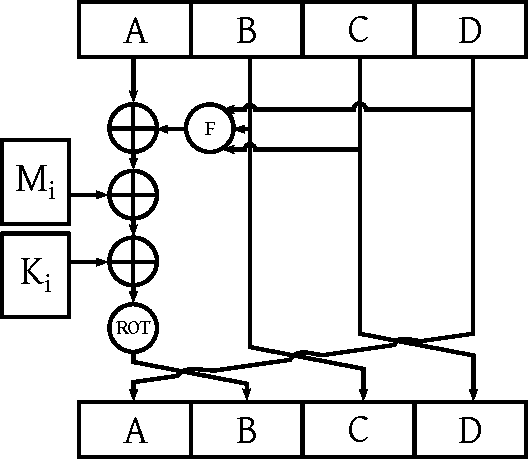
\includegraphics{img/md4.pdf}
    \caption{MD4 round function updating state variables}
    \label{fig:md4-round-function}
  \end{center}
\end{figure}











\section{SHA-256}
\label{sec:dc-sha-256}
%
\index{SHA-256}
SHA-256 is a hash function from the SHA-2 family designed by the National Security Agency (NSA)
and published as FIPS PUB 180-4 (originally 2001)~\cite{fips-pub-180-4}.
It uses a Merkle-Damg\aa{}rd construction with a Davies-Meyer compression function.
The best known preimage attack was found in 2011
and breaks preimage resistance for 52~rounds~\cite{bicliques}. The best known collision attack
breaks collision resistance for 31~rounds of SHA-256~\cite{improving} and pseudo-collision
resistance for 46~rounds~\cite{high2011}. The best practical attack is a pseudo-collision
for 38 steps~\cite{mendel2013improving}.

\begin{table}[!hb]
  \begin{center}
    \begin{tabular}{lcl}
      block size           & 512 bits   & as per Section~1 of the standard~\cite{fips-pub-180-4} \\
      digest size          & 256 bits   & mentioned as Message Digest size~\cite{fips-pub-180-4} \\
      internal state size  & 256 bits   & as per Section~1 of the standard~\cite{fips-pub-180-4} \\
      word size            & 32 bits    & as per Section~1 of the standard~\cite{fips-pub-180-4}
    \end{tabular}
    \caption{SHA-256 hash algorithm properties}
    \label{tab:sha256}
  \end{center}
\end{table}
%
\index{Left-shift}
\index{Right-shift}
\index{Left-rotation}
\index{Right-rotation}
\begin{defi}[Shifts, rotations and a notational remark]
  \label{def:shifts}
  Consider a 32-bit word $X$ with 32 binary values $b_i$ with $0 \leq i \leq 31$.
  $b_0$ refers to the least significant bit. Shifting ($≪$ and $≫$) and
  rotation ($⋘$ and $⋙$) creates a new 32-bit word $Y$ with 32 binary values $a_i$.
  We define the following notations:
  \begin{align*}
    Y \coloneqq X ≪ n  &\iff a_i \coloneqq b_{i-n} \text{ if } 0 \leq i-n < 32 \text{ and } 0 \text{ otherwise } \\
    Y \coloneqq X ≫ n  &\iff a_i \coloneqq b_{i+n} \text{ if } 0 \leq i+n < 32 \text{ and } 0 \text{ otherwise } \\
    Y \coloneqq X ⋘ n  &\iff a_i \coloneqq b_{i-n \bmod{32}} \text{ as used in MD4} \\
    Y \coloneqq X ⋙ n  &\iff a_i \coloneqq b_{i+n \bmod{32}}
  \end{align*}
\end{defi}
%
Besides MD4's \boolf{MAJ} and \boolf{IF},
another four auxiliary functions are defined. Recognize that $\oplus$ denotes
the XOR function whereas $\boxplus$ denotes 32-bit addition.
\[
  \begin{array}{rcccccl}
    \Sigma_0(X) &\coloneqq& (X ⋙ 2) &\oplus& (X ⋙ 13) &\oplus& (X ⋙ 22) \\
    \Sigma_1(X) &\coloneqq& (X ⋙ 6) &\oplus& (X ⋙ 11) &\oplus& (X ⋙ 25) \\
    \sigma_0(X) &\coloneqq& (X ⋙ 7) &\oplus& (X ⋙ 18) &\oplus& (X ≫ 3) \\
    \sigma_1(X) &\coloneqq& (X ⋙ 17) &\oplus& (X ⋙ 19) &\oplus& (X ≫ 10)
  \end{array}
\]
%
\begin{description}
  \item[Padding and length extension.]
    The padding and length extension scheme of MD4 is used also in SHA-256.
    Append bit $1$ and followed by a sequence of bit $0$ until the message reaches a length
    of 448 modulo 512 bits. Afterwards the first 64 bits of the binary representation
    of the original input are appended.
  \item[Initialization.]
    In a similar manner to MD4, initialization of internal state variables
    (called \enquote{working variables} in~\cite[Section~6.2.2]{fips-pub-180-4})
    takes place before running the round function. The eight state variables
    are initialized with the following hexadecimal values:
    \[
      \begin{array}{llll}
        A_{-1} = \texttt{6a09e667} &
        A_{-2} = \texttt{bb67ae85} &
        A_{-3} = \texttt{3c6ef372} &
        A_{-4} = \texttt{a54ff53a} \\
        E_{-1} = \texttt{510e527f} &
        E_{-2} = \texttt{9b05688c} &
        E_{-3} = \texttt{1f83d9ab} &
        E_{-4} = \texttt{5be0cd19}
      \end{array}
    \]
    Furthermore SHA-256 uses 64 constant values in its round function.
    We initialize step constants $K_i$ for $0 \leq i < 64$ with the following hexadecimal
    values (which must be read left to right and top to bottom):
    \[
      \begin{array}{cccccc}
        \texttt{428a2f98} & \texttt{71374491} & \texttt{b5c0fbcf} & \texttt{e9b5dba5} & \texttt{3956c25b} & \texttt{59f111f1} \\
        \texttt{923f82a4} & \texttt{ab1c5ed5} & \texttt{d807aa98} & \texttt{12835b01} & \texttt{243185be} & \texttt{550c7dc3} \\
        \texttt{72be5d74} & \texttt{80deb1fe} & \texttt{9bdc06a7} & \texttt{c19bf174} & \texttt{e49b69c1} & \texttt{efbe4786} \\
        \texttt{0fc19dc6} & \texttt{240ca1cc} & \texttt{2de92c6f} & \texttt{4a7484aa} & \texttt{5cb0a9dc} & \texttt{76f988da} \\
        \texttt{983e5152} & \texttt{a831c66d} & \texttt{b00327c8} & \texttt{bf597fc7} & \texttt{c6e00bf3} & \texttt{d5a79147} \\
        \texttt{06ca6351} & \texttt{14292967} & \texttt{27b70a85} & \texttt{2e1b2138} & \texttt{4d2c6dfc} & \texttt{53380d13} \\
        \texttt{650a7354} & \texttt{766a0abb} & \texttt{81c2c92e} & \texttt{92722c85} & \texttt{a2bfe8a1} & \texttt{a81a664b} \\
        \texttt{c24b8b70} & \texttt{c76c51a3} & \texttt{d192e819} & \texttt{d6990624} & \texttt{f40e3585} & \texttt{106aa070} \\
        \texttt{19a4c116} & \texttt{1e376c08} & \texttt{2748774c} & \texttt{34b0bcb5} & \texttt{391c0cb3} & \texttt{4ed8aa4a} \\
        \texttt{5b9cca4f} & \texttt{682e6ff3} & \texttt{748f82ee} & \texttt{78a5636f} & \texttt{84c87814} & \texttt{8cc70208} \\
        \texttt{90befffa} & \texttt{a4506ceb} & \texttt{bef9a3f7} & \texttt{c67178f2}
      \end{array}
    \]
  \item[Precomputation of W.]
    Let $W_i$ for $0 \leq i < 16$ be the sixteen 32-bit words of the padded input message.
    Then compute $W_i$ for $16 \leq i < 64$ the following way:
    \[ W_i \coloneqq \sigT(W_{i-2}) + W_{i-7} + \sigO(W_{i-15}) + W_{i-16} \]
  \item[Round function.]
    For every block of 512~bits, the round function is applied.
    The eight state variables are updated iteratively for $i$ from 0 to 63.
    \begin{align*}
      E_i     &\coloneqq A_{i-4} + E_{i-4} + \SigT(E_{i-1}) + \IF{(E_{i-1}, E_{i-2}, E_{i-3})} + K_i + W_i \\
      A_i     &\coloneqq E_i - A_{i-4} + \SigO(A_{i-1}) + \MAJ{(A_{i-1}, A_{i-2}, A_{i-3})}
    \end{align*}
    $W_i$ and $K_i$ refer to the previously initialized values.
  \item[Computation of intermediate hash values.]
    Intermediate hash values for the Davies-Meyer construction are
    initialized with the following values:
    \[
      \begin{array}{cp{10pt}cp{10pt}cp{10pt}c}
        H_0^{(0)} \coloneqq A_{-1}  & &  H_1^{(0)} \coloneqq A_{-2}  & &  H_2^{(0)} \coloneqq A_{-3}  & &  H_3^{(0)} \coloneqq A_{-4} \\
        H_4^{(i)} \coloneqq E_{-1}  & &  H_5^{(i)} \coloneqq E_{-2}  & &  H_6^{(i)} \coloneqq E_{-3}  & &  H_7^{(i)} \coloneqq E_{-4} \\
      \end{array}
    \]
    Every block creates its own $E_{i}$ and $A_{i}$ values for $60 \leq i < 64$.
    These are used to compute the next intermediate values:
    \[
      \begin{array}{lp{10pt}r}
        H_0^{(j)} \coloneqq A_{63} + H_0^{(i-1)}  & &  H_4^{(j)} \coloneqq E_{63} + H_4^{(i-1)} \\
        H_1^{(j)} \coloneqq A_{62} + H_1^{(i-1)}  & &  H_5^{(j)} \coloneqq E_{62} + H_5^{(i-1)} \\
        H_2^{(j)} \coloneqq A_{61} + H_2^{(i-1)}  & &  H_6^{(j)} \coloneqq E_{61} + H_6^{(i-1)} \\
        H_3^{(j)} \coloneqq A_{60} + H_3^{(i-1)}  & &  H_7^{(j)} \coloneqq E_{60} + H_7^{(i-1)}
      \end{array}
    \]
  \item[Finalization.]
    The final hash digest of size 256 bits is provided as
    \[
      H_0^{(N)} \concat
      H_1^{(N)} \concat
      H_2^{(N)} \concat
      H_3^{(N)} \concat
      H_4^{(N)} \concat
      H_5^{(N)} \concat
      H_6^{(N)} \concat
      H_7^{(N)}
    \]
    where $N$ denotes the index of the last block and operator $\|$ denotes
    concatenation. Hence $H_0^{(N)}$ are the four least significant bytes of the digest.
\end{description}

\begin{figure}[ht]
  \begin{center}
    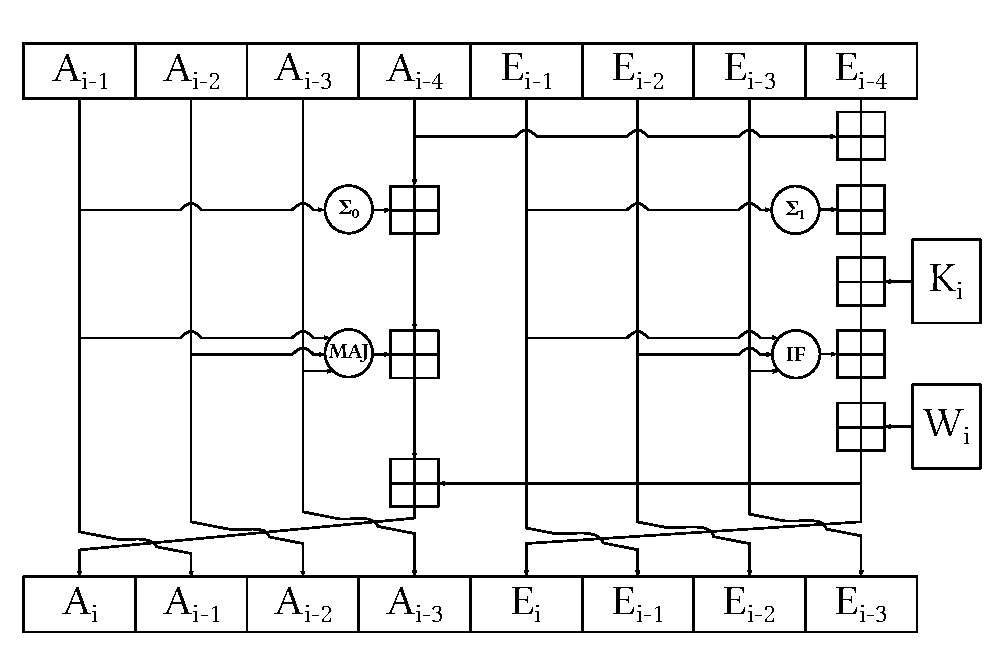
\includegraphics{img/sha256.pdf}
    \caption{SHA-256 round function~\cite{analysisSHA256}}
    \label{fig:sha256-round-function}
  \end{center}
\end{figure}

\renewcommand*\chappic{img/diff-crypt.pdf}
\renewcommand*\chapquote{Just because it's automatic doesn't mean it works.}
\renewcommand*\chapquotesrc{Daniel J. Bernstein}
%
\chapter{Differential cryptanalysis}
\label{ch:dc}
%
In Chapter~\ref{ch:hash} we defined two hash functions. In this chapter
we consider such functions from a differential perspective. Differential
cryptanalysis will turn out to yield successful collision attacks on hash
functions. We introduce a notation to easily represent differential
characteristics.

\section{Motivation}
\label{sec:dc-motivation}
%
In August 2004, Wang et al. published results at Crypto'04~\cite{wang2004} which revealed
that MD4, MD5, HAVAL-128 and RIPEMD can be broken practically using differential cryptanalysis.
Their work is based on preliminary work by Hans Dobbertin~\cite{Dobbertin1998}.
On an IBM~P690 machine, an MD5 collision can be computed in about one hour using this approach.
Collisions for HAVAL-128, MD4 and RIPEMD were found as well. Patrick Stach's \texttt{md4coll.c}
program~\cite{md4coll} implements Wang's approach and can find MD4 collisions in few seconds
on my Thinkpad~x220 setup specified in Appendix~\ref{app:setup}.

Let $n$ denote the digest size, i.e. the size of the hash value $h(x)$ in bits.
Due to the birthday paradox, a collision attack has a generic complexity of $2^{n/2}$
whereas preimage and second preimage attacks have generic complexities of $2^n$.
In other words it is computationally easier to find any two colliding hash values
than the preimage or second preimage for a given hash value.

Following results by Wang et al., differential cryptanalysis was shown as
powerful tool for cryptanalysis of hash algorithms. This thesis applies those
ideas to satisfiability approaches.

\begin{table}[bt]
  \begin{center}
    \begin{tabular}{cccc}
      \hline \hline
      \multicolumn{4}{c}{Message 1} \\
      \hline
        4d7a9c83 & \textbf{d6cb927a} & \textbf{29d5a578} & 57a7a5ee \\
        de748a3c & dcc366b3 & b683a020 & 3b2a5d9f \\
        c69d71b3 & f9e99198 & d79f805e & a63bb2e8 \\
        \textbf{45dc8e31} & 97e31fe5 & 2794bf08 & b9e8c3e9 \\
      \hline
      \multicolumn{4}{c}{Message 2} \\
      \hline
        4d7a9c83 & \textbf{56cb927a} & \textbf{b9d5a578} & 57a7a5ee \\
        de748a3c & dcc366b3 & b683a020 & 3b2a5d9f \\
        c69d71b3 & f9e99198 & d79f805e & a63bb2e8 \\
        \textbf{45dd8e31} & 97e31fe5 & 2794bf08 & b9e8c3e9 \\
      \hline
      \multicolumn{4}{c}{Hash value of Message 1 and Message 2} \\
      \hline
        5f5c1a0d & 71b36046 & 1b5435da & 9b0d807a \\
      \hline \hline
    \end{tabular}
    \caption[Hexadecimal values of one MD4 collisions given in paper~\cite{wang2004}]{
      One of two MD4 hash collisions provided in~\cite{wang2004}.
      A message represents one block of 512~bits.
      %The hash value consists of 128~bits.
      Values are given in hexadecimal, message words are enumerated from
      left to right, top to bottom. Differences are highlighted in
      bold for illustration purposes. For comparison the first bits
      of Message 1 are \texttt{11000001\dots} and the last bits are
      \texttt{\dots10011101}.
    }
    \label{tab:wang-md4-collision1}
  \end{center}
\end{table}

\newpage
\section{Fundamentals}
\label{sec:dc-fundamentals}
%
\index{Hash collision}
\begin{defi}[Hash collision]
  Given a hash function $h$,
  a hash collision is a pair $(x_1, x_2)$ with $x_1 \neq x_2$ such that
  $h(x_1) = h(x_2)$.
\end{defi}

\index{Pseudo-collision}
Pseudo-collisions are also often considered when attacking hash functions.
A \emph{pseudo-collision} is given if a hash collision can be found for a given
hash function, but the initial vectors (IV) can be chosen for each message.

Hash algorithms consume input values as blocks of bits.
As far as the length of the input must not conform to the block size,
padding is applied. Now consider such a block of input values
and another copy of it. We use those two blocks as inputs for two
hash algorithm instances, but provide slight modifications in few bits.
Differential cryptanalysis is based on the idea to consider those execution states
and trace those differences to learn about the propagation of message differences.
Compare this setup with Figure~\ref{tab:collision-attack}.

\index{Avalanche effect}
At the very beginning only the few defined differences are given. But as the
hash algorithm progresses in computation, differences are propagated to more
and more bits. Most likely the final value will differ in many bits, because
of a desirable hash algorithm property called \emph{avalanche effect}.
A small difference in the input should lead to a significant difference
in the output (i.e. visually recognizable).

Visualizing those differences helps the cryptanalyst to find modifications
yielding a small number of differences in the evaluation state. Empirical
results in differential cryptanalysis indicate that sparse characteristics
are desirable, because it is easier to cancel out few differences in the
output compared to many differences.
The cryptanalyst consecutively modifies the input values to eventually
receive a collision in the output value (i.e. $\Delta C = 0 \iff C = C^*$).

\index{Differential path}
\index{Differential characteristic}
\begin{defi}
  The differential state during a computation is called
  \emph{differential characteristic} (also \emph{differential path}).
\end{defi}

\begin{theorem}
  Assuming the number of differences in a differential characteristic is small,
  this characteristic is expected to result in a hash collision with higher probability.
\end{theorem}

\begin{figure}[bt]
  \begin{center}
    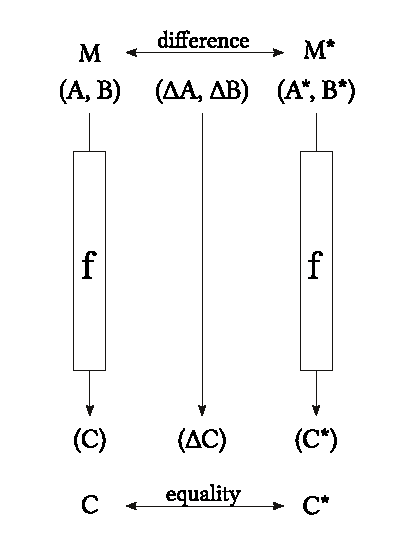
\includegraphics[width=0.55\textwidth]{img/diff_cryptanalysis.pdf}
    \caption[Common attack setting for a collision attack]{
      Common attack setting for a collision attack:
      Hash function $f$ is applied to two inputs $M$ and $M^*$ which differ
      by some predefined bits. $\Delta M$ describes the difference between
      these values. A hash collision is given if and only if output values
      $C$ and $C^*$ show the same value. In differential cryptanalysis we observe
      the differences between two instances applying function $f$
      to inputs $M$ and $M^*$.
    }
    \label{tab:collision-attack}
  \end{center}
\end{figure}

\section{Differential notation}
\label{sec:dc-notation}
%
\index{Bit condition}
\index{Generalized bit condition}
\index{Differential notation}
Differential notation helps us to visualize differential characteristics
by defining so-called \emph{generalized bit conditions}.
It was introduced by Christophe de Canni\`ere and Christian Rechberger
in 2006~\cite[Section 3.2]{char-2006}, inspired by \emph{signed differences} by
Wang~et al. and is shown in Table~\ref{tab:diff-notation}.

\begin{table}[!ht]
  \small
  \begin{center}
    \begin{tabular}{|c|cccc|}
    \hline\hline
      $(x_i, x_i^*)$ & $(0,0)$ & $(1,0)$ & $(0,1)$ & $(1,1)$ \\
    \hline
      \dnI{?}        & \yes    & \yes    & \yes    & \yes    \\
      \dnI{-}        & \yes    & \no     & \no     & \yes    \\
      \dnI{x}        & \no     & \yes    & \yes    & \no     \\
      \dnI{0}        & \yes    & \no     & \no     & \no     \\
      \dnI{u}        & \no     & \yes    & \no     & \no     \\
      \dnI{n}        & \no     & \no     & \yes    & \no     \\
      \dnI{1}        & \no     & \no     & \no     & \yes    \\
      \dnI{\#}       & \no     & \no     & \no     & \no     \\
    \hline \hline
    \end{tabular}
    \begin{tabular}{|c|cccc|}
    \hline\hline
      $(x_i, x_i^*)$ & $(0,0)$ & $(1,0)$ & $(0,1)$ & $(1,1)$ \\
    \hline
      \dnI{3}        & \yes    & \yes    & \no     & \no     \\
      \dnI{5}        & \yes    & \no     & \yes    & \no     \\
      \dnI{7}        & \yes    & \yes    & \yes    & \no     \\
      \dnI{A}        & \no     & \yes    & \no     & \yes    \\
      \dnI{B}        & \yes    & \yes    & \no     & \yes    \\
      \dnI{C}        & \no     & \no     & \yes    & \yes    \\
      \dnI{D}        & \yes    & \no     & \yes    & \yes    \\
      \dnI{E}        & \no     & \yes    & \yes    & \yes    \\
    \hline \hline
    \end{tabular}
    \caption[Differential notation as introduced in~\cite{char-2006}]{
      Differential notation as introduced in~\cite{char-2006}.
      The left-most column specifies a symbol called \enquote{bit condition}
      and right-side columns indicate which bit configurations
      are possible for two given bits $x_i$ and $x_i^*$.
    }
    \label{tab:diff-notation}
  \end{center}
\end{table}

Consider two hash algorithm instances. Let $x_i$ be some bit
from the first instance and let $x_i^*$ be the corresponding bit
from the second instance. Differences are computed using a \boolf{XOR}
and commonly denoted as $\Delta x = x_i \oplus x_i^*$.
Bit conditions allow us to encode possible relations between bits $x_i$ and $x_i^*$.

For example, let us take a look at the original Wang et al. hash collision
in MD4 provided in Table~\ref{tab:wang-md4-collision1}.
We extract all values with differences and represent them using differential notation.
This gives us Table~\ref{tab:differential-wang-values}.

\begin{table}[!ht]
  \begin{center}
    \small
    \begin{tabular}{ccl}
      \hline \hline
      bit & hexadecimal & binary representation / differential notation \\
      \hline \hline
      $x_0$ & \dnI{d6cb927a} & \dnI{11010110110010111001001001111010} \\
      $x_1$ & \dnI{29d5a578} & \dnI{00101001110101011010010101111000} \\
      $x_2$ & \dnI{45dc8e31} & \dnI{01000101110111001000111000110001} \\
      \hline
      $x_0^*$ & \dnI{56cb927a} & \dnI{01010110110010111001001001111010} \\
      $x_1^*$ & \dnI{b9d5a578} & \dnI{10111001110101011010010101111000} \\
      $x_2^*$ & \dnI{45dd8e31} & \dnI{01000101110111011000111000110001} \\
      \hline
      $\Delta x$ & & \dnI{u1010110110010111001001001111010} \\
                 & & \dnI{n01n1001110101011010010101111000} \\
                 & & \dnI{010001011101110n1000111000110001} \\
      \hline \hline
    \end{tabular}
    \caption[Bit differences in the original Wang et al. hash collision]{
      The three words different between Message~1 and Message~2 of the original
      MD4 hash collision by Wang et al. The last three lines show
      how differences can be
      written down using bit conditions. As far as 4 symbols are not from the
      set $\set{0, 1}$ it holds that the messages differ by 4~bits.
    }
    \label{tab:differential-wang-values}
  \end{center}
\end{table}

The following properties hold for bit conditions:
\begin{itemize}[noitemsep,topsep=0pt]
  \item If $x_i = x_i^*$ holds and some value is known, $\set{0,1}$ contains its bit condition.
  \item If $x_i \neq x_i^*$ holds and some value is known, $\set{u,n}$ contains its bit condition.
  \item If $x_i = x_i^*$ holds and the values are unknown, its bit condition is $\dnI{-}$.
  \item If $x_i \neq x_i^*$ holds and the values are unknown, its bit condition is $\dnI{x}$.
\end{itemize}
Applying this notation to hash collisions means that arbitrary bit conditions
(except for \dnI{\#}) can be specified for the input values. In one of the
intermediate iterations, we enforce a difference using one of the bit conditions
$\set{u,n,x}$. This excludes trivial solutions with no differences from the set of
possible solutions. And the final values need to lack differences thus are
represented using a dash \dnI{-}.

\begin{table}[!ht]
  \begin{center}
    \begin{tabular}{cp{5cm}cl}
      $\Delta x$      & conjunctive normal form &
      $\Delta x$      & conjunctive normal form \\
    \hline
      \dnI{\#}        & $(x) \land (\neg x)$ &
      \dnI{1}         & $(x) \land (x^*)$ \\

      \dnI{0}         & $(\neg x) \land (\neg x^*)$ &
      \dnI{-}         & $\neg (x \oplus x^*)$ \\

      \dnI{u}         & $(x) \land (\neg x^*)$ &
      \dnI{A}         & $(x)$ \\

      \dnI{3}         & $(\neg x^*)$ &
      \dnI{B}         & $(x \lor \neg x^*)$ \\

      \dnI{n}         & $(\neg x) \land (x^*)$ &
      \dnI{C}         & $(x^*)$ \\

      \dnI{5}         & $(\neg x)$ &
      \dnI{D}         & $(\neg x \lor x^*)$ \\

      \dnI{x}         & $(x \oplus x^*)$ &
      \dnI{E}         & $(x \lor x^*)$ \\

      \dnI{7}         & $(\neg x \lor \neg x^*)$ &
      \dnI{?}         &  \\
    \end{tabular}
    \caption[Representation of bit conditions as CNF]{%
      All bit conditions represented as CNF using
      two Boolean variables $x$ and $x^*$ to represent
      two bits.
    }
    \label{tab:simple-eval-clauses}
  \end{center}
\end{table}


\section{A simple addition example}
\label{sec:dc-example}
%
Using this notation, we can now reason about the behavior of functions on differential values.
We start with 1-bit addition as basic exercise to the reader. Consider a matrix with
two input rows and one output row. The values of the first two rows are added such that
the bit difference at the third row is created.

\begin{figure}[!ht]
  \begin{center}
    \begin{minipage}{20pt}\begin{tabular}{c} \dnI{-} \\ \dnI{-} \\ \hline \dnI{-} \end{tabular}\end{minipage}
    \hspace{20pt}$\Rightarrow$\hspace{20pt}
    \begin{minipage}{20pt}\begin{tabular}{c} \dnI{0}\dnI{0} \\ \dnI{0}\dnI{0} \\ \hline \dnI{0}\dnI{0} \end{tabular}\end{minipage}
    \begin{minipage}{20pt}\begin{tabular}{c} \dnI{0}\dnI{0} \\ \dnI{0}\dnI{0} \\ \hline \dnI{1}\dnI{1} \end{tabular}\end{minipage}
    \begin{minipage}{20pt}\begin{tabular}{c} \dnI{0}\dnI{0} \\ \dnI{1}\dnI{1} \\ \hline \dnI{0}\dnI{0} \end{tabular}\end{minipage}
    \begin{minipage}{20pt}\begin{tabular}{c} \dnI{0}\dnI{0} \\ \dnI{1}\dnI{1} \\ \hline \dnI{1}\dnI{1} \end{tabular}\end{minipage}
    \begin{minipage}{20pt}\begin{tabular}{c} \dnI{1}\dnI{1} \\ \dnI{0}\dnI{0} \\ \hline \dnI{0}\dnI{0} \end{tabular}\end{minipage}
    \begin{minipage}{20pt}\begin{tabular}{c} \dnI{1}\dnI{1} \\ \dnI{0}\dnI{0} \\ \hline \dnI{1}\dnI{1} \end{tabular}\end{minipage}
    \begin{minipage}{20pt}\begin{tabular}{c} \dnI{1}\dnI{1} \\ \dnI{1}\dnI{1} \\ \hline \dnI{0}\dnI{0} \end{tabular}\end{minipage}
    \begin{minipage}{20pt}\begin{tabular}{c} \dnI{1}\dnI{1} \\ \dnI{1}\dnI{1} \\ \hline \dnI{1}\dnI{1} \end{tabular}\end{minipage}
    \caption[A simple 1-bit addition example]{%
      A simple 1-bit addition example:
      On the left the differential characteristic is given.
      Two dashes, by definition, denote a missing difference in both arguments.
      The result of the addition must never show a difference.
      This yields eight possible bit configurations where two values close to each other denote $(M, M^*)$ of Figure~\ref{tab:collision-attack}.
      Due to the behavior of addition, we know that configurations 2, 3, 5 and 8 (from left to right) are invalid.
    }
    \label{fig:1-bit-example}
  \end{center}
\end{figure}

Figure~\ref{fig:1-bit-example} illustrates this example. Remember that symbols such as
\dnI{-} and \dnI{0} underlie semantics defined in Table~\ref{tab:diff-notation}.
It is also interesting to see how propagation of values can work. In
Figure~\ref{fig:1-bit-deduction} we see how an underspecified value \dnI{?} can be
strengthened once we have checked which values can be taken. Recognize that the
system is constrained by the function in use and the definition of the differential symbols.

\begin{figure}[!ht]
  \begin{center}
    \begin{minipage}{20pt}\begin{tabular}{c} \dnI{-} \\ \dnI{-} \\ \hline \dnI{?} \end{tabular}\end{minipage}
    \hspace{20pt}$\Rightarrow$\hspace{20pt}
    \begin{minipage}{20pt}\begin{tabular}{c} \dnI{0}\dnI{0} \\ \dnI{0}\dnI{0} \\ \hline \dnI{0}\dnI{0} \end{tabular}\end{minipage}
    \begin{minipage}{20pt}\begin{tabular}{c} \dnI{0}\dnI{0} \\ \dnI{1}\dnI{1} \\ \hline \dnI{1}\dnI{1} \end{tabular}\end{minipage}
    \begin{minipage}{20pt}\begin{tabular}{c} \dnI{1}\dnI{1} \\ \dnI{0}\dnI{0} \\ \hline \dnI{1}\dnI{1} \end{tabular}\end{minipage}
    \begin{minipage}{20pt}\begin{tabular}{c} \dnI{1}\dnI{1} \\ \dnI{1}\dnI{1} \\ \hline \dnI{0}\dnI{0} \end{tabular}\end{minipage}
    \caption[Propagation of bit conditions in a differential characteristic]{%
      Like Figure~\ref{fig:1-bit-example}, but any difference value for the result bit is possible.
      As such we consider any possible bit configuration, but eventually recognize that only four bit configurations
      are consistent with the behavior of addition. Because all resulting configurations show no bit difference
      in the output bit, we can strengthen \dnI{?} by replacing it with \dnI{-}. This illustrates how
      knowledge about differential states can be propagated.
    }
    \label{fig:1-bit-deduction}
  \end{center}
\end{figure}

Finally, we can extend our testcases to 4~bits and retrieve testcases such as
Figures~\ref{fig:4-bit-addition} and \ref{fig:sigma}.

\begin{figure}[!ht]
  \begin{center}
    \begin{minipage}{0.23\textwidth}
      \begin{tabular}{rl}
        A: & \dnI{0}\dnI{0}\dnI{1}\dnI{1} \\
        B: & \dnI{0}\dnI{1}\dnI{0}\dnI{1} \\
        S: & \dnI{1}\dnI{0}\dnI{0}\dnI{0}
      \end{tabular}
    \end{minipage}
    \begin{minipage}{0.23\textwidth}
      \begin{tabular}{rl}
        A: & \dnI{-}\dnI{-}\dnI{-}\dnI{x} \\
        B: & \dnI{-}\dnI{-}\dnI{-}\dnI{x} \\
        S: & \dnI{?}\dnI{?}\dnI{?}\dnI{?}
      \end{tabular}
    \end{minipage}
    \begin{minipage}{0.23\textwidth}
      \begin{tabular}{rl}
        A: & \dnI{-}\dnI{-}\dnI{-}\dnI{x} \\
        B: & \dnI{-}\dnI{-}\dnI{-}\dnI{x} \\
        S: & \dnI{?}\dnI{?}\dnI{?}\dnI{-}
      \end{tabular}
    \end{minipage}
    \begin{minipage}{0.23\textwidth}
      \begin{tabular}{rl}
        A: & \dnI{-}\dnI{-}\dnI{-}\dnI{x} \\
        B: & \dnI{-}\dnI{-}\dnI{-}\dnI{x} \\
        S: & \dnI{x}\dnI{?}\dnI{?}\dnI{?}
      \end{tabular}
    \end{minipage}
  \end{center}%

  \begin{center}
    \begin{minipage}{0.23\textwidth}
      \begin{tabular}{rl}
        A: & \dnI{0}\dnI{0}\dnI{1}\dnI{1} \\
        B: & \dnI{0}\dnI{1}\dnI{0}\dnI{1} \\
        S: & \dnI{0}\dnI{0}\dnI{0}\dnI{0}
      \end{tabular}
    \end{minipage}
    \begin{minipage}{0.23\textwidth}
      \begin{tabular}{rl}
        A: & \dnI{-}\dnI{-}\dnI{-}\dnI{x} \\
        B: & \dnI{-}\dnI{-}\dnI{-}\dnI{x} \\
        S: & \dnI{?}\dnI{?}\dnI{?}\dnI{x}
      \end{tabular}
    \end{minipage}
    \begin{minipage}{0.23\textwidth}
      \begin{tabular}{rl}
        A: & \dnI{-}\dnI{-}\dnI{-}\dnI{-} \\
        B: & \dnI{-}\dnI{-}\dnI{-}\dnI{x} \\
        S: & \dnI{x}\dnI{-}\dnI{?}\dnI{?}
      \end{tabular}
    \end{minipage}
  \end{center}%
  \caption[
    Testcases for 4-bit addition
  ]{
    Testcases for 4-bit addition:
    The upper line shows valid differential characteristics for 4-bit addition
    whereas the lower line show invalid ones for 4-bit addition.
    The rows are conventionally named using capital letters.
  }
  \label{fig:4-bit-addition}
\end{figure}

\begin{figure}[!ht]
  \begin{center}
    \begin{minipage}{0.23\textwidth}
      \begin{tabular}{rl}
        A: & \dnI{-}\dnI{-}\dnI{-}\dnI{-} \\
        S: & \dnI{0}\dnI{0}\dnI{0}\dnI{0}
      \end{tabular}
    \end{minipage}
    \begin{minipage}{0.23\textwidth}
      \begin{tabular}{rl}
        A: & \dnI{7}\dnI{C}\dnI{-}\dnI{3} \\
        S: & \dnI{-}\dnI{3}\dnI{u}\dnI{?}
      \end{tabular}
    \end{minipage}
    \begin{minipage}{0.23\textwidth}
      \begin{tabular}{rl}
        A: & \dnI{0}\dnI{u}\dnI{C}\dnI{D} \\
        S: & \dnI{A}\dnI{D}\dnI{C}\dnI{7} \\
      \end{tabular}
    \end{minipage}
  \end{center}

  \begin{center}
    \begin{minipage}{0.23\textwidth}
      \begin{tabular}{rl}
        A: & \dnI{-}\dnI{-}\dnI{-}\dnI{x} \\
        S: & \dnI{0}\dnI{0}\dnI{0}\dnI{0}
      \end{tabular}
    \end{minipage}
    \begin{minipage}{0.23\textwidth}
      \begin{tabular}{rl}
        A: & \dnI{x}\dnI{x}\dnI{x}\dnI{x} \\
        S: & \dnI{0}\dnI{0}\dnI{0}\dnI{0} \\
      \end{tabular}
    \end{minipage}
  \end{center}
  \caption[Differential characteristics for the SHA-2 Sigma function]{
    Differential characteristics for the SHA-2 Sigma function.
    The upper line shows valid states. The lower line shows invalid ones.
  }
  \label{fig:sigma}
\end{figure}

\section{Differential characteristics in action}
\label{sec:dc-actual-chars}
%
In the previous section, we illustrated how propagation with differential values
works and how differential characteristics are written down. It is always
important to keep in mind which function the characteristic illustrates,
because this is not documented with the characteristic.

Now consider MD4 as defined in Section~\ref{sec:dc-md4}. MD4 takes some input
message (in our case limited to size of one block), the state variables
are initialized and iteratively new $A_i$ are computed.

Similarly, SHA-256 takes a message block $M$ and initializes eight
variables with an initial vector (IV). The remaining $W_i$ are computed
and iteratively, values $A_i$ and $E_i$ are computed.

Those values are structured in differential characteristics illustrated
in Figure~\ref{img:char-layouts}. Those layouts are used to specify our
hash collisions we want to evaluate. Table~\ref{tab:wang-collision-propagated}
also gives an application of the layout.

\begin{figure}[!ht]
  \begin{center}
    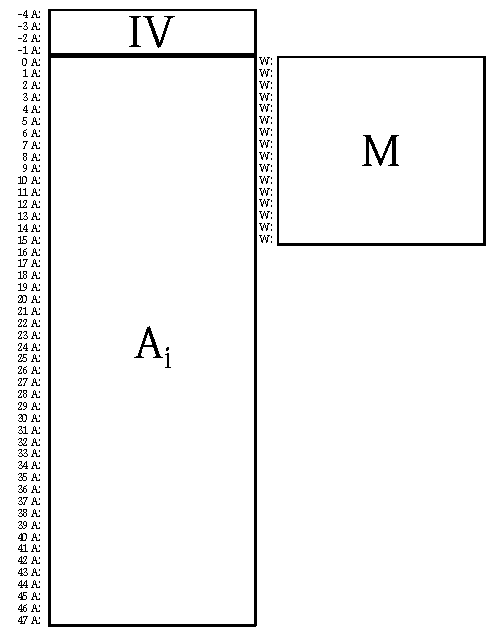
\includegraphics[width=0.4\linewidth]{img/md4_layout.pdf}
    ~~
    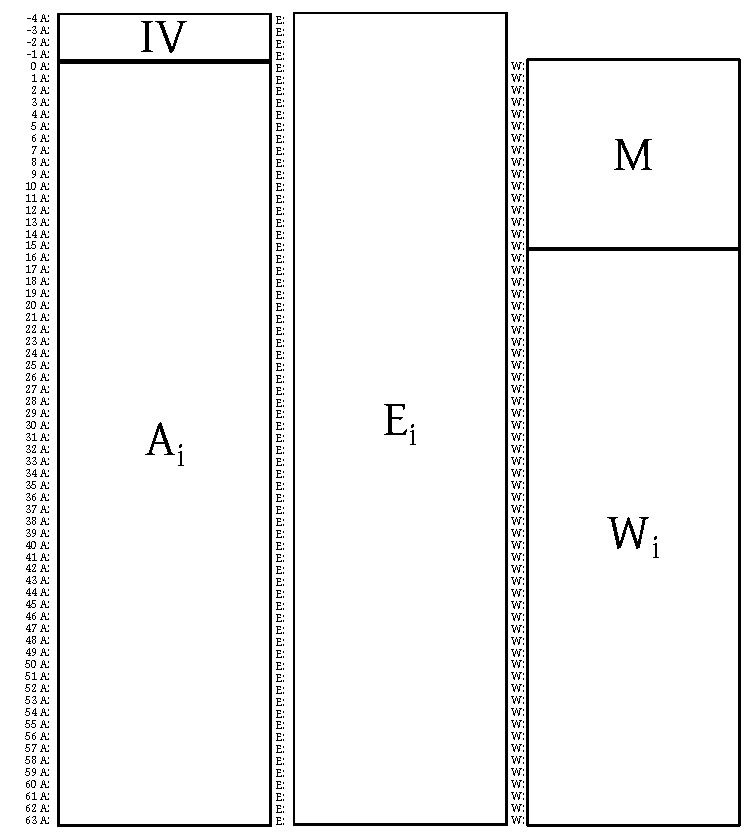
\includegraphics[width=0.5\linewidth]{img/sha256_layout.pdf}
    \caption{Layout of MD4 (left) and SHA-256 (right) differential characteristics}
    \label{img:char-layouts}
  \end{center}
\end{figure}


\texttt{
\begin{table}[p]
\begin{center}
\scalebox{.37}{
\begin{tabular}{|r|c|c|c|c|}
\hline
  $i$  &      &  $\nabla{S_{i,0}}$  &  $\nabla{S_{i,1}}$  &  $\nabla{S_{i,2}}$ \\
\hline
 \dnI{-4} & \dnW: & {{\dnCz}{\dnCo}{\dnCo}{\dnCz}{\dnCz}{\dnCo}{\dnCo}{\dnCo}{\dnCz}{\dnCo}{\dnCz}{\dnCz}{\dnCz}{\dnCo}{\dnCz}{\dnCo}{\dnCz}{\dnCz}{\dnCo}{\dnCz}{\dnCz}{\dnCz}{\dnCo}{\dnCo}{\dnCz}{\dnCz}{\dnCz}{\dnCz}{\dnCz}{\dnCz}{\dnCz}{\dnCo}} & & \\
 \dnI{-3} & \dnW: & {{\dnCz}{\dnCz}{\dnCz}{\dnCo}{\dnCz}{\dnCz}{\dnCz}{\dnCz}{\dnCz}{\dnCz}{\dnCo}{\dnCo}{\dnCz}{\dnCz}{\dnCo}{\dnCz}{\dnCz}{\dnCo}{\dnCz}{\dnCo}{\dnCz}{\dnCo}{\dnCz}{\dnCz}{\dnCz}{\dnCo}{\dnCo}{\dnCo}{\dnCz}{\dnCo}{\dnCo}{\dnCz}} & & \\
 \dnI{-2} & \dnW: & {{\dnCo}{\dnCz}{\dnCz}{\dnCo}{\dnCo}{\dnCz}{\dnCz}{\dnCz}{\dnCo}{\dnCz}{\dnCo}{\dnCo}{\dnCo}{\dnCz}{\dnCo}{\dnCz}{\dnCo}{\dnCo}{\dnCz}{\dnCo}{\dnCo}{\dnCo}{\dnCz}{\dnCz}{\dnCo}{\dnCo}{\dnCo}{\dnCo}{\dnCo}{\dnCo}{\dnCo}{\dnCz}} & & \\
 \dnI{-1} & \dnW: & {{\dnCo}{\dnCo}{\dnCo}{\dnCz}{\dnCo}{\dnCo}{\dnCo}{\dnCo}{\dnCo}{\dnCo}{\dnCz}{\dnCz}{\dnCo}{\dnCo}{\dnCz}{\dnCo}{\dnCo}{\dnCz}{\dnCo}{\dnCz}{\dnCo}{\dnCz}{\dnCo}{\dnCo}{\dnCo}{\dnCz}{\dnCz}{\dnCz}{\dnCo}{\dnCz}{\dnCz}{\dnCo}} & & \\
 \dnI{0} & \dnW: & {{\dnCz}{\dnCo}{\dnCo}{\dnCz}{\dnCo}{\dnCz}{\dnCo}{\dnCo}{\dnCo}{\dnCo}{\dnCz}{\dnCo}{\dnCz}{\dnCo}{\dnCz}{\dnCz}{\dnCo}{\dnCo}{\dnCo}{\dnCz}{\dnCz}{\dnCo}{\dnCz}{\dnCz}{\dnCz}{\dnCz}{\dnCz}{\dnCo}{\dnCz}{\dnCz}{\dnCo}{\dnCz}} & \dnW[W]{}: & {{\dnCz}{\dnCo}{\dnCz}{\dnCz}{\dnCo}{\dnCo}{\dnCz}{\dnCo}{\dnCz}{\dnCo}{\dnCo}{\dnCo}{\dnCo}{\dnCz}{\dnCo}{\dnCz}{\dnCo}{\dnCz}{\dnCz}{\dnCo}{\dnCo}{\dnCo}{\dnCz}{\dnCz}{\dnCo}{\dnCz}{\dnCz}{\dnCz}{\dnCz}{\dnCz}{\dnCo}{\dnCo}} \\
 \dnI{1} & \dnW: & {{\dnCz}{\dnCo}{\dnCo}{\dnCo}{\dnCz}{\dnCo}{\dnCo}{\dnCz}{\dnCz}{\dnCo}{\dnCz}{\dnCz}{\dnCo}{\dnCo}{\dnCo}{\dnCo}{\dnCo}{\dnCo}{\dnCo}{\dnCz}{\dnCo}{\dnCo}{\dnCo}{\dnCz}{\dnCz}{\dnCu}{\dnCo}{\dnCo}{\dnCz}{\dnCz}{\dnCz}{\dnCo}} & \dnW[W]{}: & {{\dnCu}{\dnCo}{\dnCz}{\dnCo}{\dnCz}{\dnCo}{\dnCo}{\dnCz}{\dnCo}{\dnCo}{\dnCz}{\dnCz}{\dnCo}{\dnCz}{\dnCo}{\dnCo}{\dnCo}{\dnCz}{\dnCz}{\dnCo}{\dnCz}{\dnCz}{\dnCo}{\dnCz}{\dnCz}{\dnCo}{\dnCo}{\dnCo}{\dnCo}{\dnCz}{\dnCo}{\dnCz}} \\
 \dnI{2} & \dnW: & {{\dnCo}{\dnCz}{\dnCo}{\dnCz}{\dnCo}{\dnCz}{\dnCo}{\dnCo}{\dnCz}{\dnCo}{\dnCz}{\dnCz}{\dnCz}{\dnCz}{\dnCz}{\dnCz}{\dnCz}{\dnCo}{\dnCo}{\dnCo}{\dnCz}{\dnCu}{\dnCz}{\dnCo}{\dnCn}{\dnCo}{\dnCo}{\dnCo}{\dnCz}{\dnCz}{\dnCo}{\dnCz}} & \dnW[W]{}: & {{\dnCn}{\dnCz}{\dnCo}{\dnCn}{\dnCo}{\dnCz}{\dnCz}{\dnCo}{\dnCo}{\dnCo}{\dnCz}{\dnCo}{\dnCz}{\dnCo}{\dnCz}{\dnCo}{\dnCo}{\dnCz}{\dnCo}{\dnCz}{\dnCz}{\dnCo}{\dnCz}{\dnCo}{\dnCz}{\dnCo}{\dnCo}{\dnCo}{\dnCo}{\dnCz}{\dnCz}{\dnCz}} \\
 \dnI{3} & \dnW: & {{\dnCo}{\dnCz}{\dnCo}{\dnCz}{\dnCo}{\dnCo}{\dnCu}{\dnCo}{\dnCz}{\dnCz}{\dnCo}{\dnCo}{\dnCo}{\dnCo}{\dnCz}{\dnCo}{\dnCz}{\dnCo}{\dnCz}{\dnCo}{\dnCz}{\dnCz}{\dnCo}{\dnCz}{\dnCz}{\dnCo}{\dnCz}{\dnCo}{\dnCz}{\dnCz}{\dnCz}{\dnCo}} & \dnW[W]{}: & {{\dnCz}{\dnCo}{\dnCz}{\dnCo}{\dnCz}{\dnCo}{\dnCo}{\dnCo}{\dnCo}{\dnCz}{\dnCo}{\dnCz}{\dnCz}{\dnCo}{\dnCo}{\dnCo}{\dnCo}{\dnCz}{\dnCo}{\dnCz}{\dnCz}{\dnCo}{\dnCz}{\dnCo}{\dnCo}{\dnCo}{\dnCo}{\dnCz}{\dnCo}{\dnCo}{\dnCo}{\dnCz}} \\
 \dnI{4} & \dnW: & {{\dnCz}{\dnCz}{\dnCo}{\dnCz}{\dnCo}{\dnCo}{\dnCz}{\dnCz}{\dnCz}{\dnCo}{\dnCo}{\dnCz}{\dnCz}{\dnCz}{\dnCo}{\dnCo}{\dnCz}{\dnCo}{\dnCz}{\dnCo}{\dnCz}{\dnCo}{\dnCz}{\dnCo}{\dnCo}{\dnCo}{\dnCo}{\dnCo}{\dnCz}{\dnCz}{\dnCo}{\dnCz}} & \dnW[W]{}: & {{\dnCo}{\dnCo}{\dnCz}{\dnCo}{\dnCo}{\dnCo}{\dnCo}{\dnCz}{\dnCz}{\dnCo}{\dnCo}{\dnCo}{\dnCz}{\dnCo}{\dnCz}{\dnCz}{\dnCo}{\dnCz}{\dnCz}{\dnCz}{\dnCo}{\dnCz}{\dnCo}{\dnCz}{\dnCz}{\dnCz}{\dnCo}{\dnCo}{\dnCo}{\dnCo}{\dnCz}{\dnCz}} \\
 \dnI{5} & \dnW: & {{\dnCz}{\dnCz}{\dnCz}{\dnCo}{\dnCo}{\dnCz}{\dnCo}{\dnCz}{\dnCz}{\dnCo}{\dnCo}{\dnCz}{\dnCz}{\dnCz}{\dnCo}{\dnCz}{\dnCo}{\dnCz}{\dnCu}{\dnCo}{\dnCo}{\dnCz}{\dnCo}{\dnCz}{\dnCz}{\dnCz}{\dnCz}{\dnCz}{\dnCz}{\dnCz}{\dnCz}{\dnCo}} & \dnW[W]{}: & {{\dnCo}{\dnCo}{\dnCz}{\dnCo}{\dnCo}{\dnCo}{\dnCz}{\dnCz}{\dnCo}{\dnCo}{\dnCz}{\dnCz}{\dnCz}{\dnCz}{\dnCo}{\dnCo}{\dnCz}{\dnCo}{\dnCo}{\dnCz}{\dnCz}{\dnCo}{\dnCo}{\dnCz}{\dnCo}{\dnCz}{\dnCo}{\dnCo}{\dnCz}{\dnCz}{\dnCo}{\dnCo}} \\
 \dnI{6} & \dnW: & {{\dnCz}{\dnCz}{\dnCz}{\dnCo}{\dnCo}{\dnCz}{\dnCo}{\dnCo}{\dnCz}{\dnCz}{\dnCu}{\dnCn}{\dnCu}{\dnCu}{\dnCo}{\dnCo}{\dnCz}{\dnCz}{\dnCz}{\dnCo}{\dnCz}{\dnCz}{\dnCz}{\dnCz}{\dnCz}{\dnCo}{\dnCo}{\dnCo}{\dnCo}{\dnCz}{\dnCo}{\dnCz}} & \dnW[W]{}: & {{\dnCq}{\dnCq}{\dnCq}{\dnCq}{\dnCq}{\dnCq}{\dnCq}{\dnCq}{\dnCq}{\dnCq}{\dnCq}{\dnCq}{\dnCq}{\dnCq}{\dnCq}{\dnCq}{\dnCq}{\dnCq}{\dnCq}{\dnCq}{\dnCq}{\dnCq}{\dnCq}{\dnCq}{\dnCq}{\dnCq}{\dnCq}{\dnCq}{\dnCq}{\dnCq}{\dnCq}{\dnCq}} \\
 \dnI{7} & \dnW: & {{\dnCz}{\dnCz}{\dnCo}{\dnCz}{\dnCo}{\dnCz}{\dnCo}{\dnCo}{\dnCo}{\dnCz}{\dnCz}{\dnCz}{\dnCz}{\dnCz}{\dnCz}{\dnCo}{\dnCz}{\dnCu}{\dnCn}{\dnCn}{\dnCz}{\dnCo}{\dnCo}{\dnCz}{\dnCz}{\dnCo}{\dnCz}{\dnCo}{\dnCz}{\dnCz}{\dnCz}{\dnCz}} & \dnW[W]{}: & {{\dnCz}{\dnCz}{\dnCo}{\dnCo}{\dnCo}{\dnCz}{\dnCo}{\dnCo}{\dnCz}{\dnCz}{\dnCo}{\dnCz}{\dnCo}{\dnCz}{\dnCo}{\dnCz}{\dnCz}{\dnCo}{\dnCz}{\dnCo}{\dnCo}{\dnCo}{\dnCz}{\dnCo}{\dnCo}{\dnCz}{\dnCz}{\dnCo}{\dnCo}{\dnCo}{\dnCo}{\dnCo}} \\
 \dnI{8} & \dnW: & {{\dnCq}{\dnCq}{\dnCq}{\dnCq}{\dnCq}{\dnCq}{\dnCq}{\dnCq}{\dnCq}{\dnCq}{\dnCq}{\dnCq}{\dnCq}{\dnCq}{\dnCq}{\dnCq}{\dnCq}{\dnCq}{\dnCq}{\dnCq}{\dnCq}{\dnCq}{\dnCq}{\dnCq}{\dnCq}{\dnCq}{\dnCq}{\dnCq}{\dnCq}{\dnCq}{\dnCq}{\dnCq}} & \dnW[W]{}: & {{\dnCo}{\dnCo}{\dnCz}{\dnCz}{\dnCz}{\dnCo}{\dnCo}{\dnCz}{\dnCo}{\dnCz}{\dnCz}{\dnCo}{\dnCo}{\dnCo}{\dnCz}{\dnCo}{\dnCz}{\dnCo}{\dnCo}{\dnCo}{\dnCz}{\dnCz}{\dnCz}{\dnCo}{\dnCo}{\dnCz}{\dnCo}{\dnCo}{\dnCz}{\dnCz}{\dnCo}{\dnCo}} \\
 \dnI{9} & \dnW: & {{\dnCq}{\dnCq}{\dnCq}{\dnCq}{\dnCq}{\dnCq}{\dnCq}{\dnCq}{\dnCq}{\dnCq}{\dnCq}{\dnCq}{\dnCq}{\dnCq}{\dnCq}{\dnCq}{\dnCq}{\dnCq}{\dnCq}{\dnCq}{\dnCq}{\dnCq}{\dnCq}{\dnCq}{\dnCq}{\dnCq}{\dnCq}{\dnCq}{\dnCq}{\dnCq}{\dnCq}{\dnCq}} & \dnW[W]{}: & {{\dnCo}{\dnCo}{\dnCo}{\dnCo}{\dnCo}{\dnCz}{\dnCz}{\dnCo}{\dnCo}{\dnCo}{\dnCo}{\dnCz}{\dnCo}{\dnCz}{\dnCz}{\dnCo}{\dnCo}{\dnCz}{\dnCz}{\dnCo}{\dnCz}{\dnCz}{\dnCz}{\dnCo}{\dnCo}{\dnCz}{\dnCz}{\dnCo}{\dnCo}{\dnCz}{\dnCz}{\dnCz}} \\
 \dnI{10} & \dnW: & {{\dnCo}{\dnCz}{\dnCn}{\dnCz}{\dnCz}{\dnCo}{\dnCz}{\dnCz}{\dnCo}{\dnCz}{\dnCz}{\dnCz}{\dnCz}{\dnCo}{\dnCz}{\dnCo}{\dnCq}{\dnCq}{\dnCq}{\dnCq}{\dnCq}{\dnCq}{\dnCq}{\dnCq}{\dnCq}{\dnCq}{\dnCq}{\dnCq}{\dnCq}{\dnCo}{\dnCo}{\dnCz}} & \dnW[W]{}: & {{\dnCo}{\dnCo}{\dnCz}{\dnCo}{\dnCz}{\dnCo}{\dnCo}{\dnCo}{\dnCo}{\dnCz}{\dnCz}{\dnCo}{\dnCo}{\dnCo}{\dnCo}{\dnCo}{\dnCo}{\dnCz}{\dnCz}{\dnCz}{\dnCz}{\dnCz}{\dnCz}{\dnCz}{\dnCz}{\dnCo}{\dnCz}{\dnCo}{\dnCo}{\dnCo}{\dnCo}{\dnCz}} \\
 \dnI{11} & \dnW: & {{\dnCu}{\dnCo}{\dnCz}{\dnCz}{\dnCz}{\dnCo}{\dnCo}{\dnCz}{\dnCo}{\dnCz}{\dnCo}{\dnCo}{\dnCz}{\dnCo}{\dnCo}{\dnCz}{\dnCq}{\dnCq}{\dnCq}{\dnCq}{\dnCq}{\dnCq}{\dnCq}{\dnCq}{\dnCq}{\dnCq}{\dnCq}{\dnCq}{\dnCq}{\dnCo}{\dnCo}{\dnCo}} & \dnW[W]{}: & {{\dnCo}{\dnCz}{\dnCo}{\dnCz}{\dnCz}{\dnCo}{\dnCo}{\dnCz}{\dnCz}{\dnCz}{\dnCo}{\dnCo}{\dnCo}{\dnCz}{\dnCo}{\dnCo}{\dnCo}{\dnCz}{\dnCo}{\dnCo}{\dnCz}{\dnCz}{\dnCo}{\dnCz}{\dnCo}{\dnCo}{\dnCo}{\dnCz}{\dnCo}{\dnCz}{\dnCz}{\dnCz}} \\
 \dnI{12} & \dnW: & {{\dnCz}{\dnCz}{\dnCo}{\dnCz}{\dnCo}{\dnCo}{\dnCu}{\dnCz}{\dnCz}{\dnCu}{\dnCo}{\dnCz}{\dnCo}{\dnCz}{\dnCo}{\dnCo}{\dnCq}{\dnCq}{\dnCq}{\dnCq}{\dnCq}{\dnCq}{\dnCq}{\dnCq}{\dnCq}{\dnCq}{\dnCq}{\dnCq}{\dnCq}{\dnCz}{\dnCo}{\dnCo}} & \dnW[W]{}: & {{\dnCz}{\dnCo}{\dnCz}{\dnCz}{\dnCz}{\dnCo}{\dnCz}{\dnCo}{\dnCo}{\dnCo}{\dnCz}{\dnCo}{\dnCo}{\dnCo}{\dnCz}{\dnCn}{\dnCo}{\dnCz}{\dnCz}{\dnCz}{\dnCo}{\dnCo}{\dnCo}{\dnCz}{\dnCz}{\dnCz}{\dnCo}{\dnCo}{\dnCz}{\dnCz}{\dnCz}{\dnCo}} \\
 \dnI{13} & \dnW: & {{\dnCo}{\dnCz}{\dnCu}{\dnCn}{\dnCo}{\dnCn}{\dnCz}{\dnCo}{\dnCz}{\dnCz}{\dnCo}{\dnCo}{\dnCz}{\dnCz}{\dnCz}{\dnCo}{\dnCq}{\dnCq}{\dnCq}{\dnCq}{\dnCq}{\dnCq}{\dnCq}{\dnCq}{\dnCq}{\dnCq}{\dnCq}{\dnCq}{\dnCq}{\dnCo}{\dnCz}{\dnCo}} & \dnW[W]{}: & {{\dnCo}{\dnCz}{\dnCz}{\dnCo}{\dnCz}{\dnCo}{\dnCo}{\dnCo}{\dnCo}{\dnCo}{\dnCo}{\dnCz}{\dnCz}{\dnCz}{\dnCo}{\dnCo}{\dnCz}{\dnCz}{\dnCz}{\dnCo}{\dnCo}{\dnCo}{\dnCo}{\dnCo}{\dnCo}{\dnCo}{\dnCo}{\dnCz}{\dnCz}{\dnCo}{\dnCz}{\dnCo}} \\
 \dnI{14} & \dnW: & {{\dnCz}{\dnCz}{\dnCz}{\dnCz}{\dnCo}{\dnCz}{\dnCo}{\dnCz}{\dnCz}{\dnCo}{\dnCz}{\dnCo}{\dnCz}{\dnCz}{\dnCz}{\dnCo}{\dnCh}{\dnCh}{\dnCh}{\dnCh}{\dnCh}{\dnCh}{\dnCh}{\dnCh}{\dnCh}{\dnCh}{\dnCh}{\dnCh}{\dnCh}{\dnCo}{\dnCo}{\dnCz}} & \dnW[W]{}: & {{\dnCz}{\dnCz}{\dnCo}{\dnCz}{\dnCz}{\dnCo}{\dnCo}{\dnCo}{\dnCo}{\dnCz}{\dnCz}{\dnCo}{\dnCz}{\dnCo}{\dnCz}{\dnCz}{\dnCo}{\dnCz}{\dnCo}{\dnCo}{\dnCo}{\dnCo}{\dnCo}{\dnCo}{\dnCz}{\dnCz}{\dnCz}{\dnCz}{\dnCo}{\dnCz}{\dnCz}{\dnCz}} \\
 \dnI{15} & \dnW: & {{\dnCz}{\dnCz}{\dnCz}{\dnCo}{\dnCo}{\dnCo}{\dnCo}{\dnCz}{\dnCo}{\dnCz}{\dnCo}{\dnCz}{\dnCo}{\dnCu}{\dnCz}{\dnCo}{\dnCh}{\dnCh}{\dnCh}{\dnCh}{\dnCh}{\dnCh}{\dnCh}{\dnCh}{\dnCh}{\dnCh}{\dnCh}{\dnCh}{\dnCh}{\dnCo}{\dnCz}{\dnCz}} & \dnW[W]{}: & {{\dnCo}{\dnCz}{\dnCo}{\dnCo}{\dnCo}{\dnCz}{\dnCz}{\dnCo}{\dnCo}{\dnCo}{\dnCo}{\dnCz}{\dnCo}{\dnCz}{\dnCz}{\dnCz}{\dnCo}{\dnCo}{\dnCz}{\dnCz}{\dnCz}{\dnCz}{\dnCo}{\dnCo}{\dnCo}{\dnCo}{\dnCo}{\dnCz}{\dnCo}{\dnCz}{\dnCz}{\dnCo}} \\
 \dnI{16} & \dnW: & {{\dnCn}{\dnCz}{\dnCz}{\dnCn}{\dnCz}{\dnCu}{\dnCn}{\dnCz}{\dnCo}{\dnCo}{\dnCz}{\dnCo}{\dnCz}{\dnCz}{\dnCo}{\dnCz}{\dnCh}{\dnCh}{\dnCh}{\dnCh}{\dnCh}{\dnCh}{\dnCh}{\dnCh}{\dnCh}{\dnCh}{\dnCh}{\dnCh}{\dnCh}{\dnCo}{\dnCo}{\dnCo}} & & \\
 \dnI{17} & \dnW: & {{\dnCz}{\dnCz}{\dnCz}{\dnCo}{\dnCo}{\dnCo}{\dnCo}{\dnCo}{\dnCz}{\dnCz}{\dnCo}{\dnCo}{\dnCo}{\dnCz}{\dnCo}{\dnCz}{\dnCh}{\dnCh}{\dnCh}{\dnCh}{\dnCh}{\dnCh}{\dnCh}{\dnCh}{\dnCh}{\dnCh}{\dnCh}{\dnCh}{\dnCh}{\dnCo}{\dnCo}{\dnCz}} & & \\
 \dnI{18} & \dnW: & {{\dnCz}{\dnCo}{\dnCz}{\dnCo}{\dnCz}{\dnCo}{\dnCo}{\dnCo}{\dnCz}{\dnCz}{\dnCz}{\dnCz}{\dnCo}{\dnCo}{\dnCz}{\dnCo}{\dnCh}{\dnCh}{\dnCh}{\dnCh}{\dnCh}{\dnCh}{\dnCh}{\dnCh}{\dnCh}{\dnCh}{\dnCh}{\dnCh}{\dnCh}{\dnCo}{\dnCz}{\dnCz}} & & \\
 \dnI{19} & \dnW: & {{\dnCu}{\dnCo}{\dnCn}{\dnCo}{\dnCz}{\dnCz}{\dnCz}{\dnCz}{\dnCz}{\dnCz}{\dnCz}{\dnCo}{\dnCz}{\dnCo}{\dnCo}{\dnCo}{\dnCh}{\dnCh}{\dnCh}{\dnCh}{\dnCh}{\dnCh}{\dnCh}{\dnCh}{\dnCh}{\dnCh}{\dnCh}{\dnCh}{\dnCh}{\dnCo}{\dnCz}{\dnCz}} & & \\
 \dnI{20} & \dnW: & {{\dnCn}{\dnCo}{\dnCu}{\dnCn}{\dnCo}{\dnCz}{\dnCz}{\dnCo}{\dnCo}{\dnCo}{\dnCo}{\dnCo}{\dnCo}{\dnCo}{\dnCz}{\dnCo}{\dnCo}{\dnCo}{\dnCz}{\dnCo}{\dnCz}{\dnCz}{\dnCz}{\dnCz}{\dnCz}{\dnCz}{\dnCo}{\dnCo}{\dnCz}{\dnCo}{\dnCz}{\dnCz}} & & \\
 \dnI{21} & \dnW: & {{\dnCo}{\dnCo}{\dnCo}{\dnCo}{\dnCz}{\dnCz}{\dnCo}{\dnCo}{\dnCo}{\dnCz}{\dnCo}{\dnCo}{\dnCz}{\dnCz}{\dnCz}{\dnCz}{\dnCz}{\dnCo}{\dnCz}{\dnCo}{\dnCo}{\dnCo}{\dnCo}{\dnCo}{\dnCo}{\dnCo}{\dnCz}{\dnCo}{\dnCz}{\dnCo}{\dnCz}{\dnCz}} & & \\
 \dnI{22} & \dnW: & {{\dnCz}{\dnCo}{\dnCz}{\dnCo}{\dnCo}{\dnCo}{\dnCz}{\dnCo}{\dnCo}{\dnCo}{\dnCz}{\dnCz}{\dnCo}{\dnCo}{\dnCz}{\dnCo}{\dnCz}{\dnCz}{\dnCo}{\dnCo}{\dnCz}{\dnCz}{\dnCo}{\dnCo}{\dnCz}{\dnCz}{\dnCo}{\dnCo}{\dnCo}{\dnCz}{\dnCo}{\dnCz}} & & \\
 \dnI{23} & \dnW: & {{\dnCz}{\dnCo}{\dnCz}{\dnCo}{\dnCz}{\dnCz}{\dnCz}{\dnCz}{\dnCo}{\dnCo}{\dnCo}{\dnCz}{\dnCo}{\dnCo}{\dnCo}{\dnCz}{\dnCo}{\dnCo}{\dnCz}{\dnCz}{\dnCz}{\dnCo}{\dnCo}{\dnCo}{\dnCo}{\dnCz}{\dnCz}{\dnCz}{\dnCo}{\dnCo}{\dnCo}{\dnCo}} & & \\
 \dnI{24} & \dnW: & {{\dnCz}{\dnCz}{\dnCz}{\dnCz}{\dnCz}{\dnCz}{\dnCo}{\dnCz}{\dnCz}{\dnCz}{\dnCz}{\dnCo}{\dnCz}{\dnCz}{\dnCo}{\dnCz}{\dnCz}{\dnCz}{\dnCo}{\dnCo}{\dnCz}{\dnCo}{\dnCo}{\dnCo}{\dnCz}{\dnCz}{\dnCz}{\dnCo}{\dnCo}{\dnCz}{\dnCo}{\dnCz}} & & \\
 \dnI{25} & \dnW: & {{\dnCo}{\dnCz}{\dnCo}{\dnCo}{\dnCz}{\dnCz}{\dnCz}{\dnCz}{\dnCo}{\dnCz}{\dnCz}{\dnCo}{\dnCz}{\dnCo}{\dnCo}{\dnCz}{\dnCz}{\dnCz}{\dnCz}{\dnCo}{\dnCz}{\dnCo}{\dnCz}{\dnCz}{\dnCo}{\dnCo}{\dnCo}{\dnCz}{\dnCo}{\dnCz}{\dnCo}{\dnCz}} & & \\
 \dnI{26} & \dnW: & {{\dnCz}{\dnCz}{\dnCz}{\dnCz}{\dnCo}{\dnCz}{\dnCo}{\dnCz}{\dnCo}{\dnCz}{\dnCz}{\dnCz}{\dnCo}{\dnCz}{\dnCz}{\dnCo}{\dnCz}{\dnCo}{\dnCo}{\dnCo}{\dnCz}{\dnCo}{\dnCo}{\dnCo}{\dnCz}{\dnCo}{\dnCz}{\dnCz}{\dnCz}{\dnCz}{\dnCz}{\dnCo}} & & \\
 \dnI{27} & \dnW: & {{\dnCz}{\dnCz}{\dnCz}{\dnCz}{\dnCz}{\dnCo}{\dnCo}{\dnCz}{\dnCo}{\dnCo}{\dnCo}{\dnCz}{\dnCo}{\dnCo}{\dnCo}{\dnCo}{\dnCz}{\dnCo}{\dnCz}{\dnCo}{\dnCo}{\dnCz}{\dnCo}{\dnCz}{\dnCo}{\dnCz}{\dnCo}{\dnCo}{\dnCz}{\dnCz}{\dnCo}{\dnCo}} & & \\
 \dnI{28} & \dnW: & {{\dnCo}{\dnCz}{\dnCo}{\dnCo}{\dnCz}{\dnCo}{\dnCo}{\dnCz}{\dnCz}{\dnCo}{\dnCz}{\dnCo}{\dnCo}{\dnCo}{\dnCz}{\dnCo}{\dnCz}{\dnCo}{\dnCo}{\dnCz}{\dnCo}{\dnCo}{\dnCz}{\dnCz}{\dnCz}{\dnCz}{\dnCo}{\dnCz}{\dnCz}{\dnCo}{\dnCz}{\dnCo}} & & \\
 \dnI{29} & \dnW: & {{\dnCo}{\dnCz}{\dnCo}{\dnCz}{\dnCz}{\dnCz}{\dnCo}{\dnCz}{\dnCz}{\dnCz}{\dnCz}{\dnCz}{\dnCo}{\dnCo}{\dnCz}{\dnCo}{\dnCz}{\dnCo}{\dnCz}{\dnCz}{\dnCo}{\dnCz}{\dnCz}{\dnCz}{\dnCz}{\dnCo}{\dnCo}{\dnCz}{\dnCo}{\dnCz}{\dnCz}{\dnCo}} & & \\
 \dnI{30} & \dnW: & {{\dnCz}{\dnCz}{\dnCo}{\dnCz}{\dnCo}{\dnCz}{\dnCz}{\dnCo}{\dnCo}{\dnCo}{\dnCz}{\dnCo}{\dnCz}{\dnCo}{\dnCo}{\dnCo}{\dnCo}{\dnCo}{\dnCz}{\dnCz}{\dnCz}{\dnCo}{\dnCo}{\dnCo}{\dnCz}{\dnCo}{\dnCo}{\dnCz}{\dnCz}{\dnCz}{\dnCo}{\dnCo}} & & \\
 \dnI{31} & \dnW: & {{\dnCo}{\dnCo}{\dnCo}{\dnCo}{\dnCo}{\dnCo}{\dnCz}{\dnCz}{\dnCo}{\dnCz}{\dnCz}{\dnCo}{\dnCz}{\dnCz}{\dnCo}{\dnCz}{\dnCo}{\dnCo}{\dnCz}{\dnCo}{\dnCz}{\dnCo}{\dnCo}{\dnCo}{\dnCo}{\dnCz}{\dnCo}{\dnCo}{\dnCz}{\dnCo}{\dnCo}{\dnCz}} & & \\
 \dnI{32} & \dnW: & {{\dnCz}{\dnCo}{\dnCz}{\dnCz}{\dnCo}{\dnCo}{\dnCo}{\dnCo}{\dnCo}{\dnCo}{\dnCz}{\dnCo}{\dnCz}{\dnCz}{\dnCo}{\dnCz}{\dnCz}{\dnCo}{\dnCo}{\dnCz}{\dnCo}{\dnCz}{\dnCz}{\dnCz}{\dnCz}{\dnCz}{\dnCo}{\dnCz}{\dnCo}{\dnCo}{\dnCo}{\dnCo}} & & \\
 \dnI{33} & \dnW: & {{\dnCz}{\dnCz}{\dnCo}{\dnCo}{\dnCo}{\dnCz}{\dnCz}{\dnCz}{\dnCz}{\dnCz}{\dnCo}{\dnCo}{\dnCo}{\dnCo}{\dnCz}{\dnCo}{\dnCz}{\dnCo}{\dnCo}{\dnCz}{\dnCo}{\dnCo}{\dnCo}{\dnCz}{\dnCo}{\dnCo}{\dnCo}{\dnCz}{\dnCz}{\dnCo}{\dnCz}{\dnCz}} & & \\
 \dnI{34} & \dnW: & {{\dnCz}{\dnCz}{\dnCo}{\dnCz}{\dnCz}{\dnCz}{\dnCz}{\dnCz}{\dnCz}{\dnCo}{\dnCo}{\dnCo}{\dnCz}{\dnCo}{\dnCz}{\dnCo}{\dnCo}{\dnCo}{\dnCo}{\dnCz}{\dnCo}{\dnCz}{\dnCz}{\dnCz}{\dnCz}{\dnCz}{\dnCz}{\dnCo}{\dnCz}{\dnCo}{\dnCz}{\dnCo}} & & \\
 \dnI{35} & \dnW: & {{\dnCn}{\dnCz}{\dnCo}{\dnCz}{\dnCz}{\dnCz}{\dnCz}{\dnCz}{\dnCz}{\dnCz}{\dnCo}{\dnCo}{\dnCz}{\dnCz}{\dnCo}{\dnCo}{\dnCz}{\dnCz}{\dnCz}{\dnCz}{\dnCz}{\dnCo}{\dnCz}{\dnCz}{\dnCz}{\dnCo}{\dnCo}{\dnCo}{\dnCz}{\dnCz}{\dnCo}{\dnCz}} & & \\
 \dnI{36} & \dnW: & {{\dnCn}{\dnCz}{\dnCz}{\dnCz}{\dnCz}{\dnCo}{\dnCo}{\dnCo}{\dnCo}{\dnCo}{\dnCo}{\dnCz}{\dnCo}{\dnCz}{\dnCo}{\dnCo}{\dnCo}{\dnCo}{\dnCz}{\dnCo}{\dnCo}{\dnCo}{\dnCo}{\dnCz}{\dnCz}{\dnCo}{\dnCz}{\dnCo}{\dnCo}{\dnCz}{\dnCz}{\dnCo}} & & \\
 \dnI{37} & \dnW: & {{\dnCo}{\dnCo}{\dnCz}{\dnCz}{\dnCo}{\dnCz}{\dnCz}{\dnCz}{\dnCz}{\dnCz}{\dnCz}{\dnCo}{\dnCo}{\dnCz}{\dnCo}{\dnCz}{\dnCz}{\dnCo}{\dnCz}{\dnCz}{\dnCz}{\dnCz}{\dnCo}{\dnCo}{\dnCz}{\dnCz}{\dnCz}{\dnCz}{\dnCo}{\dnCo}{\dnCz}{\dnCz}} & & \\
 \dnI{38} & \dnW: & {{\dnCo}{\dnCz}{\dnCo}{\dnCo}{\dnCz}{\dnCz}{\dnCz}{\dnCz}{\dnCz}{\dnCo}{\dnCo}{\dnCz}{\dnCz}{\dnCo}{\dnCo}{\dnCo}{\dnCo}{\dnCo}{\dnCo}{\dnCz}{\dnCo}{\dnCz}{\dnCz}{\dnCo}{\dnCo}{\dnCz}{\dnCo}{\dnCz}{\dnCo}{\dnCo}{\dnCz}{\dnCz}} & & \\
 \dnI{39} & \dnW: & {{\dnCz}{\dnCz}{\dnCz}{\dnCo}{\dnCz}{\dnCz}{\dnCo}{\dnCz}{\dnCz}{\dnCz}{\dnCz}{\dnCz}{\dnCo}{\dnCz}{\dnCo}{\dnCz}{\dnCz}{\dnCz}{\dnCz}{\dnCo}{\dnCo}{\dnCz}{\dnCo}{\dnCo}{\dnCz}{\dnCz}{\dnCz}{\dnCo}{\dnCo}{\dnCo}{\dnCz}{\dnCz}} & & \\
 \dnI{40} & \dnW: & {{\dnCo}{\dnCo}{\dnCz}{\dnCz}{\dnCz}{\dnCz}{\dnCz}{\dnCz}{\dnCz}{\dnCo}{\dnCz}{\dnCz}{\dnCo}{\dnCz}{\dnCz}{\dnCz}{\dnCz}{\dnCo}{\dnCo}{\dnCo}{\dnCz}{\dnCz}{\dnCz}{\dnCo}{\dnCo}{\dnCz}{\dnCz}{\dnCz}{\dnCz}{\dnCo}{\dnCz}{\dnCo}} & & \\
 \dnI{41} & \dnW: & {{\dnCz}{\dnCz}{\dnCz}{\dnCz}{\dnCz}{\dnCo}{\dnCo}{\dnCz}{\dnCo}{\dnCz}{\dnCz}{\dnCz}{\dnCz}{\dnCo}{\dnCo}{\dnCz}{\dnCo}{\dnCo}{\dnCo}{\dnCo}{\dnCz}{\dnCo}{\dnCz}{\dnCo}{\dnCz}{\dnCz}{\dnCo}{\dnCz}{\dnCz}{\dnCo}{\dnCo}{\dnCz}} & & \\
 \dnI{42} & \dnW: & {{\dnCz}{\dnCo}{\dnCz}{\dnCz}{\dnCo}{\dnCo}{\dnCo}{\dnCz}{\dnCo}{\dnCo}{\dnCz}{\dnCo}{\dnCo}{\dnCo}{\dnCz}{\dnCo}{\dnCo}{\dnCo}{\dnCo}{\dnCo}{\dnCo}{\dnCo}{\dnCo}{\dnCz}{\dnCo}{\dnCz}{\dnCz}{\dnCz}{\dnCz}{\dnCo}{\dnCo}{\dnCz}} & & \\
 \dnI{43} & \dnW: & {{\dnCz}{\dnCo}{\dnCz}{\dnCo}{\dnCz}{\dnCz}{\dnCz}{\dnCz}{\dnCz}{\dnCo}{\dnCo}{\dnCz}{\dnCz}{\dnCz}{\dnCo}{\dnCo}{\dnCo}{\dnCo}{\dnCz}{\dnCo}{\dnCz}{\dnCz}{\dnCz}{\dnCz}{\dnCz}{\dnCo}{\dnCo}{\dnCz}{\dnCo}{\dnCo}{\dnCz}{\dnCo}} & & \\
 \dnI{44} & \dnW: & {{\dnCo}{\dnCo}{\dnCo}{\dnCo}{\dnCo}{\dnCz}{\dnCz}{\dnCz}{\dnCz}{\dnCz}{\dnCz}{\dnCo}{\dnCz}{\dnCo}{\dnCo}{\dnCz}{\dnCo}{\dnCo}{\dnCo}{\dnCo}{\dnCz}{\dnCo}{\dnCo}{\dnCo}{\dnCz}{\dnCz}{\dnCz}{\dnCz}{\dnCo}{\dnCo}{\dnCz}{\dnCz}} & & \\
 \dnI{45} & \dnW: & {{\dnCo}{\dnCz}{\dnCz}{\dnCz}{\dnCo}{\dnCz}{\dnCo}{\dnCz}{\dnCo}{\dnCo}{\dnCz}{\dnCo}{\dnCo}{\dnCz}{\dnCo}{\dnCo}{\dnCz}{\dnCz}{\dnCo}{\dnCz}{\dnCo}{\dnCo}{\dnCz}{\dnCz}{\dnCz}{\dnCz}{\dnCz}{\dnCz}{\dnCz}{\dnCo}{\dnCz}{\dnCz}} & & \\
 \dnI{46} & \dnW: & {{\dnCo}{\dnCz}{\dnCz}{\dnCz}{\dnCz}{\dnCz}{\dnCo}{\dnCz}{\dnCo}{\dnCz}{\dnCz}{\dnCo}{\dnCo}{\dnCz}{\dnCz}{\dnCo}{\dnCz}{\dnCo}{\dnCz}{\dnCo}{\dnCo}{\dnCz}{\dnCz}{\dnCz}{\dnCo}{\dnCo}{\dnCz}{\dnCo}{\dnCo}{\dnCo}{\dnCz}{\dnCz}} & & \\
 \dnI{47} & \dnW: & {{\dnCo}{\dnCz}{\dnCz}{\dnCz}{\dnCz}{\dnCz}{\dnCz}{\dnCo}{\dnCo}{\dnCo}{\dnCo}{\dnCz}{\dnCz}{\dnCo}{\dnCz}{\dnCo}{\dnCo}{\dnCz}{\dnCo}{\dnCo}{\dnCz}{\dnCo}{\dnCz}{\dnCz}{\dnCo}{\dnCz}{\dnCo}{\dnCo}{\dnCo}{\dnCo}{\dnCz}{\dnCo}} & & \\
\hline
\end{tabular}
\hspace{10pt}$\Rightarrow$\hspace{10pt}
\begin{tabular}{|r|c|c|c|c|}
\hline
  $i$  &      &  $\nabla{S_{i,0}}$  &  $\nabla{S_{i,1}}$  &  $\nabla{S_{i,2}}$ \\
\hline
 \dnI{-4} & \dnW: & {{\dnCz}{\dnCo}{\dnCo}{\dnCz}{\dnCz}{\dnCo}{\dnCo}{\dnCo}{\dnCz}{\dnCo}{\dnCz}{\dnCz}{\dnCz}{\dnCo}{\dnCz}{\dnCo}{\dnCz}{\dnCz}{\dnCo}{\dnCz}{\dnCz}{\dnCz}{\dnCo}{\dnCo}{\dnCz}{\dnCz}{\dnCz}{\dnCz}{\dnCz}{\dnCz}{\dnCz}{\dnCo}} & & \\
 \dnI{-3} & \dnW: & {{\dnCz}{\dnCz}{\dnCz}{\dnCo}{\dnCz}{\dnCz}{\dnCz}{\dnCz}{\dnCz}{\dnCz}{\dnCo}{\dnCo}{\dnCz}{\dnCz}{\dnCo}{\dnCz}{\dnCz}{\dnCo}{\dnCz}{\dnCo}{\dnCz}{\dnCo}{\dnCz}{\dnCz}{\dnCz}{\dnCo}{\dnCo}{\dnCo}{\dnCz}{\dnCo}{\dnCo}{\dnCz}} & & \\
 \dnI{-2} & \dnW: & {{\dnCo}{\dnCz}{\dnCz}{\dnCo}{\dnCo}{\dnCz}{\dnCz}{\dnCz}{\dnCo}{\dnCz}{\dnCo}{\dnCo}{\dnCo}{\dnCz}{\dnCo}{\dnCz}{\dnCo}{\dnCo}{\dnCz}{\dnCo}{\dnCo}{\dnCo}{\dnCz}{\dnCz}{\dnCo}{\dnCo}{\dnCo}{\dnCo}{\dnCo}{\dnCo}{\dnCo}{\dnCz}} & & \\
 \dnI{-1} & \dnW: & {{\dnCo}{\dnCo}{\dnCo}{\dnCz}{\dnCo}{\dnCo}{\dnCo}{\dnCo}{\dnCo}{\dnCo}{\dnCz}{\dnCz}{\dnCo}{\dnCo}{\dnCz}{\dnCo}{\dnCo}{\dnCz}{\dnCo}{\dnCz}{\dnCo}{\dnCz}{\dnCo}{\dnCo}{\dnCo}{\dnCz}{\dnCz}{\dnCz}{\dnCo}{\dnCz}{\dnCz}{\dnCo}} & & \\
 \dnI{0} & \dnW: & {{\dnCz}{\dnCo}{\dnCo}{\dnCz}{\dnCo}{\dnCz}{\dnCo}{\dnCo}{\dnCo}{\dnCo}{\dnCz}{\dnCo}{\dnCz}{\dnCo}{\dnCz}{\dnCz}{\dnCo}{\dnCo}{\dnCo}{\dnCz}{\dnCz}{\dnCo}{\dnCz}{\dnCz}{\dnCz}{\dnCz}{\dnCz}{\dnCo}{\dnCz}{\dnCz}{\dnCo}{\dnCz}} & \dnW[W]{}: & {{\dnCz}{\dnCo}{\dnCz}{\dnCz}{\dnCo}{\dnCo}{\dnCz}{\dnCo}{\dnCz}{\dnCo}{\dnCo}{\dnCo}{\dnCo}{\dnCz}{\dnCo}{\dnCz}{\dnCo}{\dnCz}{\dnCz}{\dnCo}{\dnCo}{\dnCo}{\dnCz}{\dnCz}{\dnCo}{\dnCz}{\dnCz}{\dnCz}{\dnCz}{\dnCz}{\dnCo}{\dnCo}} \\
 \dnI{1} & \dnW: & {{\dnCz}{\dnCo}{\dnCo}{\dnCo}{\dnCz}{\dnCo}{\dnCo}{\dnCz}{\dnCz}{\dnCo}{\dnCz}{\dnCz}{\dnCo}{\dnCo}{\dnCo}{\dnCo}{\dnCo}{\dnCo}{\dnCo}{\dnCz}{\dnCo}{\dnCo}{\dnCo}{\dnCz}{\dnCz}{\dnCu}{\dnCo}{\dnCo}{\dnCz}{\dnCz}{\dnCz}{\dnCo}} & \dnW[W]{}: & {{\dnCu}{\dnCo}{\dnCz}{\dnCo}{\dnCz}{\dnCo}{\dnCo}{\dnCz}{\dnCo}{\dnCo}{\dnCz}{\dnCz}{\dnCo}{\dnCz}{\dnCo}{\dnCo}{\dnCo}{\dnCz}{\dnCz}{\dnCo}{\dnCz}{\dnCz}{\dnCo}{\dnCz}{\dnCz}{\dnCo}{\dnCo}{\dnCo}{\dnCo}{\dnCz}{\dnCo}{\dnCz}} \\
 \dnI{2} & \dnW: & {{\dnCo}{\dnCz}{\dnCo}{\dnCz}{\dnCo}{\dnCz}{\dnCo}{\dnCo}{\dnCz}{\dnCo}{\dnCz}{\dnCz}{\dnCz}{\dnCz}{\dnCz}{\dnCz}{\dnCz}{\dnCo}{\dnCo}{\dnCo}{\dnCz}{\dnCu}{\dnCz}{\dnCo}{\dnCn}{\dnCo}{\dnCo}{\dnCo}{\dnCz}{\dnCz}{\dnCo}{\dnCz}} & \dnW[W]{}: & {{\dnCn}{\dnCz}{\dnCo}{\dnCn}{\dnCo}{\dnCz}{\dnCz}{\dnCo}{\dnCo}{\dnCo}{\dnCz}{\dnCo}{\dnCz}{\dnCo}{\dnCz}{\dnCo}{\dnCo}{\dnCz}{\dnCo}{\dnCz}{\dnCz}{\dnCo}{\dnCz}{\dnCo}{\dnCz}{\dnCo}{\dnCo}{\dnCo}{\dnCo}{\dnCz}{\dnCz}{\dnCz}} \\
 \dnI{3} & \dnW: & {{\dnCo}{\dnCz}{\dnCo}{\dnCz}{\dnCo}{\dnCo}{\dnCu}{\dnCo}{\dnCz}{\dnCz}{\dnCo}{\dnCo}{\dnCo}{\dnCo}{\dnCz}{\dnCo}{\dnCz}{\dnCo}{\dnCz}{\dnCo}{\dnCz}{\dnCz}{\dnCo}{\dnCz}{\dnCz}{\dnCo}{\dnCz}{\dnCo}{\dnCz}{\dnCz}{\dnCz}{\dnCo}} & \dnW[W]{}: & {{\dnCz}{\dnCo}{\dnCz}{\dnCo}{\dnCz}{\dnCo}{\dnCo}{\dnCo}{\dnCo}{\dnCz}{\dnCo}{\dnCz}{\dnCz}{\dnCo}{\dnCo}{\dnCo}{\dnCo}{\dnCz}{\dnCo}{\dnCz}{\dnCz}{\dnCo}{\dnCz}{\dnCo}{\dnCo}{\dnCo}{\dnCo}{\dnCz}{\dnCo}{\dnCo}{\dnCo}{\dnCz}} \\
 \dnI{4} & \dnW: & {{\dnCz}{\dnCz}{\dnCo}{\dnCz}{\dnCo}{\dnCo}{\dnCz}{\dnCz}{\dnCz}{\dnCo}{\dnCo}{\dnCz}{\dnCz}{\dnCz}{\dnCo}{\dnCo}{\dnCz}{\dnCo}{\dnCz}{\dnCo}{\dnCz}{\dnCo}{\dnCz}{\dnCo}{\dnCo}{\dnCo}{\dnCo}{\dnCo}{\dnCz}{\dnCz}{\dnCo}{\dnCz}} & \dnW[W]{}: & {{\dnCo}{\dnCo}{\dnCz}{\dnCo}{\dnCo}{\dnCo}{\dnCo}{\dnCz}{\dnCz}{\dnCo}{\dnCo}{\dnCo}{\dnCz}{\dnCo}{\dnCz}{\dnCz}{\dnCo}{\dnCz}{\dnCz}{\dnCz}{\dnCo}{\dnCz}{\dnCo}{\dnCz}{\dnCz}{\dnCz}{\dnCo}{\dnCo}{\dnCo}{\dnCo}{\dnCz}{\dnCz}} \\
 \dnI{5} & \dnW: & {{\dnCz}{\dnCz}{\dnCz}{\dnCo}{\dnCo}{\dnCz}{\dnCo}{\dnCz}{\dnCz}{\dnCo}{\dnCo}{\dnCz}{\dnCz}{\dnCz}{\dnCo}{\dnCz}{\dnCo}{\dnCz}{\dnCu}{\dnCo}{\dnCo}{\dnCz}{\dnCo}{\dnCz}{\dnCz}{\dnCz}{\dnCz}{\dnCz}{\dnCz}{\dnCz}{\dnCz}{\dnCo}} & \dnW[W]{}: & {{\dnCo}{\dnCo}{\dnCz}{\dnCo}{\dnCo}{\dnCo}{\dnCz}{\dnCz}{\dnCo}{\dnCo}{\dnCz}{\dnCz}{\dnCz}{\dnCz}{\dnCo}{\dnCo}{\dnCz}{\dnCo}{\dnCo}{\dnCz}{\dnCz}{\dnCo}{\dnCo}{\dnCz}{\dnCo}{\dnCz}{\dnCo}{\dnCo}{\dnCz}{\dnCz}{\dnCo}{\dnCo}} \\
 \dnI{6} & \dnW: & {{\dnCz}{\dnCz}{\dnCz}{\dnCo}{\dnCo}{\dnCz}{\dnCo}{\dnCo}{\dnCz}{\dnCz}{\dnCu}{\dnCn}{\dnCu}{\dnCu}{\dnCo}{\dnCo}{\dnCz}{\dnCz}{\dnCz}{\dnCo}{\dnCz}{\dnCz}{\dnCz}{\dnCz}{\dnCz}{\dnCo}{\dnCo}{\dnCo}{\dnCo}{\dnCz}{\dnCo}{\dnCz}} & \dnW[W]{}: & {{\dnCo}{\dnCz}{\dnCo}{\dnCo}{\dnCz}{\dnCo}{\dnCo}{\dnCz}{\dnCo}{\dnCz}{\dnCz}{\dnCz}{\dnCz}{\dnCz}{\dnCo}{\dnCo}{\dnCo}{\dnCz}{\dnCo}{\dnCz}{\dnCz}{\dnCz}{\dnCz}{\dnCz}{\dnCz}{\dnCz}{\dnCo}{\dnCz}{\dnCz}{\dnCz}{\dnCz}{\dnCz}} \\
 \dnI{7} & \dnW: & {{\dnCz}{\dnCz}{\dnCo}{\dnCz}{\dnCo}{\dnCz}{\dnCo}{\dnCo}{\dnCo}{\dnCz}{\dnCz}{\dnCz}{\dnCz}{\dnCz}{\dnCz}{\dnCo}{\dnCz}{\dnCu}{\dnCn}{\dnCn}{\dnCz}{\dnCo}{\dnCo}{\dnCz}{\dnCz}{\dnCo}{\dnCz}{\dnCo}{\dnCz}{\dnCz}{\dnCz}{\dnCz}} & \dnW[W]{}: & {{\dnCz}{\dnCz}{\dnCo}{\dnCo}{\dnCo}{\dnCz}{\dnCo}{\dnCo}{\dnCz}{\dnCz}{\dnCo}{\dnCz}{\dnCo}{\dnCz}{\dnCo}{\dnCz}{\dnCz}{\dnCo}{\dnCz}{\dnCo}{\dnCo}{\dnCo}{\dnCz}{\dnCo}{\dnCo}{\dnCz}{\dnCz}{\dnCo}{\dnCo}{\dnCo}{\dnCo}{\dnCo}} \\
 \dnI{8} & \dnW: & {{\dnCz}{\dnCo}{\dnCo}{\dnCo}{\dnCz}{\dnCz}{\dnCo}{\dnCo}{\dnCz}{\dnCz}{\dnCo}{\dnCz}{\dnCz}{\dnCz}{\dnCo}{\dnCu}{\dnCo}{\dnCo}{\dnCo}{\dnCo}{\dnCo}{\dnCo}{\dnCo}{\dnCo}{\dnCo}{\dnCz}{\dnCo}{\dnCo}{\dnCz}{\dnCz}{\dnCz}{\dnCz}} & \dnW[W]{}: & {{\dnCo}{\dnCo}{\dnCz}{\dnCz}{\dnCz}{\dnCo}{\dnCo}{\dnCz}{\dnCo}{\dnCz}{\dnCz}{\dnCo}{\dnCo}{\dnCo}{\dnCz}{\dnCo}{\dnCz}{\dnCo}{\dnCo}{\dnCo}{\dnCz}{\dnCz}{\dnCz}{\dnCo}{\dnCo}{\dnCz}{\dnCo}{\dnCo}{\dnCz}{\dnCz}{\dnCo}{\dnCo}} \\
 \dnI{9} & \dnW: & {{\dnCo}{\dnCz}{\dnCo}{\dnCz}{\dnCo}{\dnCo}{\dnCn}{\dnCz}{\dnCo}{\dnCu}{\dnCn}{\dnCn}{\dnCu}{\dnCz}{\dnCz}{\dnCz}{\dnCo}{\dnCo}{\dnCo}{\dnCo}{\dnCo}{\dnCz}{\dnCz}{\dnCo}{\dnCo}{\dnCz}{\dnCz}{\dnCo}{\dnCo}{\dnCo}{\dnCo}{\dnCo}} & \dnW[W]{}: & {{\dnCo}{\dnCo}{\dnCo}{\dnCo}{\dnCo}{\dnCz}{\dnCz}{\dnCo}{\dnCo}{\dnCo}{\dnCo}{\dnCz}{\dnCo}{\dnCz}{\dnCz}{\dnCo}{\dnCo}{\dnCz}{\dnCz}{\dnCo}{\dnCz}{\dnCz}{\dnCz}{\dnCo}{\dnCo}{\dnCz}{\dnCz}{\dnCo}{\dnCo}{\dnCz}{\dnCz}{\dnCz}} \\
 \dnI{10} & \dnW: & {{\dnCo}{\dnCz}{\dnCn}{\dnCz}{\dnCz}{\dnCo}{\dnCz}{\dnCz}{\dnCo}{\dnCz}{\dnCz}{\dnCz}{\dnCz}{\dnCo}{\dnCz}{\dnCo}{\dnCz}{\dnCo}{\dnCz}{\dnCz}{\dnCz}{\dnCz}{\dnCz}{\dnCz}{\dnCo}{\dnCz}{\dnCo}{\dnCz}{\dnCo}{\dnCo}{\dnCo}{\dnCz}} & \dnW[W]{}: & {{\dnCo}{\dnCo}{\dnCz}{\dnCo}{\dnCz}{\dnCo}{\dnCo}{\dnCo}{\dnCo}{\dnCz}{\dnCz}{\dnCo}{\dnCo}{\dnCo}{\dnCo}{\dnCo}{\dnCo}{\dnCz}{\dnCz}{\dnCz}{\dnCz}{\dnCz}{\dnCz}{\dnCz}{\dnCz}{\dnCo}{\dnCz}{\dnCo}{\dnCo}{\dnCo}{\dnCo}{\dnCz}} \\
 \dnI{11} & \dnW: & {{\dnCu}{\dnCo}{\dnCz}{\dnCz}{\dnCz}{\dnCo}{\dnCo}{\dnCz}{\dnCo}{\dnCz}{\dnCo}{\dnCo}{\dnCz}{\dnCo}{\dnCo}{\dnCz}{\dnCz}{\dnCo}{\dnCz}{\dnCz}{\dnCo}{\dnCz}{\dnCo}{\dnCz}{\dnCo}{\dnCo}{\dnCo}{\dnCo}{\dnCo}{\dnCo}{\dnCo}{\dnCo}} & \dnW[W]{}: & {{\dnCo}{\dnCz}{\dnCo}{\dnCz}{\dnCz}{\dnCo}{\dnCo}{\dnCz}{\dnCz}{\dnCz}{\dnCo}{\dnCo}{\dnCo}{\dnCz}{\dnCo}{\dnCo}{\dnCo}{\dnCz}{\dnCo}{\dnCo}{\dnCz}{\dnCz}{\dnCo}{\dnCz}{\dnCo}{\dnCo}{\dnCo}{\dnCz}{\dnCo}{\dnCz}{\dnCz}{\dnCz}} \\
 \dnI{12} & \dnW: & {{\dnCz}{\dnCz}{\dnCo}{\dnCz}{\dnCo}{\dnCo}{\dnCu}{\dnCz}{\dnCz}{\dnCu}{\dnCo}{\dnCz}{\dnCo}{\dnCz}{\dnCo}{\dnCo}{\dnCo}{\dnCo}{\dnCo}{\dnCo}{\dnCo}{\dnCo}{\dnCz}{\dnCz}{\dnCz}{\dnCo}{\dnCo}{\dnCo}{\dnCo}{\dnCz}{\dnCo}{\dnCo}} & \dnW[W]{}: & {{\dnCz}{\dnCo}{\dnCz}{\dnCz}{\dnCz}{\dnCo}{\dnCz}{\dnCo}{\dnCo}{\dnCo}{\dnCz}{\dnCo}{\dnCo}{\dnCo}{\dnCz}{\dnCn}{\dnCo}{\dnCz}{\dnCz}{\dnCz}{\dnCo}{\dnCo}{\dnCo}{\dnCz}{\dnCz}{\dnCz}{\dnCo}{\dnCo}{\dnCz}{\dnCz}{\dnCz}{\dnCo}} \\
 \dnI{13} & \dnW: & {{\dnCo}{\dnCz}{\dnCu}{\dnCn}{\dnCo}{\dnCn}{\dnCz}{\dnCo}{\dnCz}{\dnCz}{\dnCo}{\dnCo}{\dnCz}{\dnCz}{\dnCz}{\dnCo}{\dnCz}{\dnCo}{\dnCz}{\dnCz}{\dnCz}{\dnCz}{\dnCz}{\dnCo}{\dnCo}{\dnCo}{\dnCo}{\dnCz}{\dnCz}{\dnCo}{\dnCz}{\dnCo}} & \dnW[W]{}: & {{\dnCo}{\dnCz}{\dnCz}{\dnCo}{\dnCz}{\dnCo}{\dnCo}{\dnCo}{\dnCo}{\dnCo}{\dnCo}{\dnCz}{\dnCz}{\dnCz}{\dnCo}{\dnCo}{\dnCz}{\dnCz}{\dnCz}{\dnCo}{\dnCo}{\dnCo}{\dnCo}{\dnCo}{\dnCo}{\dnCo}{\dnCo}{\dnCz}{\dnCz}{\dnCo}{\dnCz}{\dnCo}} \\
 \dnI{14} & \dnW: & {{\dnCz}{\dnCz}{\dnCz}{\dnCz}{\dnCo}{\dnCz}{\dnCo}{\dnCz}{\dnCz}{\dnCo}{\dnCz}{\dnCo}{\dnCz}{\dnCz}{\dnCz}{\dnCo}{\dnCo}{\dnCz}{\dnCz}{\dnCz}{\dnCo}{\dnCz}{\dnCz}{\dnCz}{\dnCo}{\dnCo}{\dnCz}{\dnCo}{\dnCz}{\dnCo}{\dnCo}{\dnCz}} & \dnW[W]{}: & {{\dnCz}{\dnCz}{\dnCo}{\dnCz}{\dnCz}{\dnCo}{\dnCo}{\dnCo}{\dnCo}{\dnCz}{\dnCz}{\dnCo}{\dnCz}{\dnCo}{\dnCz}{\dnCz}{\dnCo}{\dnCz}{\dnCo}{\dnCo}{\dnCo}{\dnCo}{\dnCo}{\dnCo}{\dnCz}{\dnCz}{\dnCz}{\dnCz}{\dnCo}{\dnCz}{\dnCz}{\dnCz}} \\
 \dnI{15} & \dnW: & {{\dnCz}{\dnCz}{\dnCz}{\dnCo}{\dnCo}{\dnCo}{\dnCo}{\dnCz}{\dnCo}{\dnCz}{\dnCo}{\dnCz}{\dnCo}{\dnCu}{\dnCz}{\dnCo}{\dnCz}{\dnCo}{\dnCo}{\dnCz}{\dnCz}{\dnCo}{\dnCo}{\dnCz}{\dnCo}{\dnCo}{\dnCz}{\dnCo}{\dnCz}{\dnCo}{\dnCz}{\dnCz}} & \dnW[W]{}: & {{\dnCo}{\dnCz}{\dnCo}{\dnCo}{\dnCo}{\dnCz}{\dnCz}{\dnCo}{\dnCo}{\dnCo}{\dnCo}{\dnCz}{\dnCo}{\dnCz}{\dnCz}{\dnCz}{\dnCo}{\dnCo}{\dnCz}{\dnCz}{\dnCz}{\dnCz}{\dnCo}{\dnCo}{\dnCo}{\dnCo}{\dnCo}{\dnCz}{\dnCo}{\dnCz}{\dnCz}{\dnCo}} \\
 \dnI{16} & \dnW: & {{\dnCn}{\dnCz}{\dnCz}{\dnCn}{\dnCz}{\dnCu}{\dnCn}{\dnCz}{\dnCo}{\dnCo}{\dnCz}{\dnCo}{\dnCz}{\dnCz}{\dnCo}{\dnCz}{\dnCo}{\dnCz}{\dnCz}{\dnCo}{\dnCo}{\dnCz}{\dnCo}{\dnCo}{\dnCz}{\dnCo}{\dnCz}{\dnCo}{\dnCo}{\dnCo}{\dnCo}{\dnCo}} & & \\
 \dnI{17} & \dnW: & {{\dnCz}{\dnCz}{\dnCz}{\dnCo}{\dnCo}{\dnCo}{\dnCo}{\dnCo}{\dnCz}{\dnCz}{\dnCo}{\dnCo}{\dnCo}{\dnCz}{\dnCo}{\dnCz}{\dnCz}{\dnCz}{\dnCz}{\dnCo}{\dnCz}{\dnCz}{\dnCo}{\dnCz}{\dnCz}{\dnCz}{\dnCz}{\dnCo}{\dnCo}{\dnCo}{\dnCo}{\dnCz}} & & \\
 \dnI{18} & \dnW: & {{\dnCz}{\dnCo}{\dnCz}{\dnCo}{\dnCz}{\dnCo}{\dnCo}{\dnCo}{\dnCz}{\dnCz}{\dnCz}{\dnCz}{\dnCo}{\dnCo}{\dnCz}{\dnCo}{\dnCz}{\dnCz}{\dnCz}{\dnCz}{\dnCz}{\dnCz}{\dnCz}{\dnCz}{\dnCo}{\dnCz}{\dnCz}{\dnCo}{\dnCz}{\dnCo}{\dnCz}{\dnCz}} & & \\
 \dnI{19} & \dnW: & {{\dnCu}{\dnCo}{\dnCn}{\dnCo}{\dnCz}{\dnCz}{\dnCz}{\dnCz}{\dnCz}{\dnCz}{\dnCz}{\dnCo}{\dnCz}{\dnCo}{\dnCo}{\dnCo}{\dnCo}{\dnCz}{\dnCz}{\dnCo}{\dnCo}{\dnCz}{\dnCo}{\dnCz}{\dnCo}{\dnCo}{\dnCz}{\dnCz}{\dnCz}{\dnCo}{\dnCz}{\dnCz}} & & \\
 \dnI{20} & \dnW: & {{\dnCn}{\dnCo}{\dnCu}{\dnCn}{\dnCo}{\dnCz}{\dnCz}{\dnCo}{\dnCo}{\dnCo}{\dnCo}{\dnCo}{\dnCo}{\dnCo}{\dnCz}{\dnCo}{\dnCo}{\dnCo}{\dnCz}{\dnCo}{\dnCz}{\dnCz}{\dnCz}{\dnCz}{\dnCz}{\dnCz}{\dnCo}{\dnCo}{\dnCz}{\dnCo}{\dnCz}{\dnCz}} & & \\
 \dnI{21} & \dnW: & {{\dnCo}{\dnCo}{\dnCo}{\dnCo}{\dnCz}{\dnCz}{\dnCo}{\dnCo}{\dnCo}{\dnCz}{\dnCo}{\dnCo}{\dnCz}{\dnCz}{\dnCz}{\dnCz}{\dnCz}{\dnCo}{\dnCz}{\dnCo}{\dnCo}{\dnCo}{\dnCo}{\dnCo}{\dnCo}{\dnCo}{\dnCz}{\dnCo}{\dnCz}{\dnCo}{\dnCz}{\dnCz}} & & \\
 \dnI{22} & \dnW: & {{\dnCz}{\dnCo}{\dnCz}{\dnCo}{\dnCo}{\dnCo}{\dnCz}{\dnCo}{\dnCo}{\dnCo}{\dnCz}{\dnCz}{\dnCo}{\dnCo}{\dnCz}{\dnCo}{\dnCz}{\dnCz}{\dnCo}{\dnCo}{\dnCz}{\dnCz}{\dnCo}{\dnCo}{\dnCz}{\dnCz}{\dnCo}{\dnCo}{\dnCo}{\dnCz}{\dnCo}{\dnCz}} & & \\
 \dnI{23} & \dnW: & {{\dnCz}{\dnCo}{\dnCz}{\dnCo}{\dnCz}{\dnCz}{\dnCz}{\dnCz}{\dnCo}{\dnCo}{\dnCo}{\dnCz}{\dnCo}{\dnCo}{\dnCo}{\dnCz}{\dnCo}{\dnCo}{\dnCz}{\dnCz}{\dnCz}{\dnCo}{\dnCo}{\dnCo}{\dnCo}{\dnCz}{\dnCz}{\dnCz}{\dnCo}{\dnCo}{\dnCo}{\dnCo}} & & \\
 \dnI{24} & \dnW: & {{\dnCz}{\dnCz}{\dnCz}{\dnCz}{\dnCz}{\dnCz}{\dnCo}{\dnCz}{\dnCz}{\dnCz}{\dnCz}{\dnCo}{\dnCz}{\dnCz}{\dnCo}{\dnCz}{\dnCz}{\dnCz}{\dnCo}{\dnCo}{\dnCz}{\dnCo}{\dnCo}{\dnCo}{\dnCz}{\dnCz}{\dnCz}{\dnCo}{\dnCo}{\dnCz}{\dnCo}{\dnCz}} & & \\
 \dnI{25} & \dnW: & {{\dnCo}{\dnCz}{\dnCo}{\dnCo}{\dnCz}{\dnCz}{\dnCz}{\dnCz}{\dnCo}{\dnCz}{\dnCz}{\dnCo}{\dnCz}{\dnCo}{\dnCo}{\dnCz}{\dnCz}{\dnCz}{\dnCz}{\dnCo}{\dnCz}{\dnCo}{\dnCz}{\dnCz}{\dnCo}{\dnCo}{\dnCo}{\dnCz}{\dnCo}{\dnCz}{\dnCo}{\dnCz}} & & \\
 \dnI{26} & \dnW: & {{\dnCz}{\dnCz}{\dnCz}{\dnCz}{\dnCo}{\dnCz}{\dnCo}{\dnCz}{\dnCo}{\dnCz}{\dnCz}{\dnCz}{\dnCo}{\dnCz}{\dnCz}{\dnCo}{\dnCz}{\dnCo}{\dnCo}{\dnCo}{\dnCz}{\dnCo}{\dnCo}{\dnCo}{\dnCz}{\dnCo}{\dnCz}{\dnCz}{\dnCz}{\dnCz}{\dnCz}{\dnCo}} & & \\
 \dnI{27} & \dnW: & {{\dnCz}{\dnCz}{\dnCz}{\dnCz}{\dnCz}{\dnCo}{\dnCo}{\dnCz}{\dnCo}{\dnCo}{\dnCo}{\dnCz}{\dnCo}{\dnCo}{\dnCo}{\dnCo}{\dnCz}{\dnCo}{\dnCz}{\dnCo}{\dnCo}{\dnCz}{\dnCo}{\dnCz}{\dnCo}{\dnCz}{\dnCo}{\dnCo}{\dnCz}{\dnCz}{\dnCo}{\dnCo}} & & \\
 \dnI{28} & \dnW: & {{\dnCo}{\dnCz}{\dnCo}{\dnCo}{\dnCz}{\dnCo}{\dnCo}{\dnCz}{\dnCz}{\dnCo}{\dnCz}{\dnCo}{\dnCo}{\dnCo}{\dnCz}{\dnCo}{\dnCz}{\dnCo}{\dnCo}{\dnCz}{\dnCo}{\dnCo}{\dnCz}{\dnCz}{\dnCz}{\dnCz}{\dnCo}{\dnCz}{\dnCz}{\dnCo}{\dnCz}{\dnCo}} & & \\
 \dnI{29} & \dnW: & {{\dnCo}{\dnCz}{\dnCo}{\dnCz}{\dnCz}{\dnCz}{\dnCo}{\dnCz}{\dnCz}{\dnCz}{\dnCz}{\dnCz}{\dnCo}{\dnCo}{\dnCz}{\dnCo}{\dnCz}{\dnCo}{\dnCz}{\dnCz}{\dnCo}{\dnCz}{\dnCz}{\dnCz}{\dnCz}{\dnCo}{\dnCo}{\dnCz}{\dnCo}{\dnCz}{\dnCz}{\dnCo}} & & \\
 \dnI{30} & \dnW: & {{\dnCz}{\dnCz}{\dnCo}{\dnCz}{\dnCo}{\dnCz}{\dnCz}{\dnCo}{\dnCo}{\dnCo}{\dnCz}{\dnCo}{\dnCz}{\dnCo}{\dnCo}{\dnCo}{\dnCo}{\dnCo}{\dnCz}{\dnCz}{\dnCz}{\dnCo}{\dnCo}{\dnCo}{\dnCz}{\dnCo}{\dnCo}{\dnCz}{\dnCz}{\dnCz}{\dnCo}{\dnCo}} & & \\
 \dnI{31} & \dnW: & {{\dnCo}{\dnCo}{\dnCo}{\dnCo}{\dnCo}{\dnCo}{\dnCz}{\dnCz}{\dnCo}{\dnCz}{\dnCz}{\dnCo}{\dnCz}{\dnCz}{\dnCo}{\dnCz}{\dnCo}{\dnCo}{\dnCz}{\dnCo}{\dnCz}{\dnCo}{\dnCo}{\dnCo}{\dnCo}{\dnCz}{\dnCo}{\dnCo}{\dnCz}{\dnCo}{\dnCo}{\dnCz}} & & \\
 \dnI{32} & \dnW: & {{\dnCz}{\dnCo}{\dnCz}{\dnCz}{\dnCo}{\dnCo}{\dnCo}{\dnCo}{\dnCo}{\dnCo}{\dnCz}{\dnCo}{\dnCz}{\dnCz}{\dnCo}{\dnCz}{\dnCz}{\dnCo}{\dnCo}{\dnCz}{\dnCo}{\dnCz}{\dnCz}{\dnCz}{\dnCz}{\dnCz}{\dnCo}{\dnCz}{\dnCo}{\dnCo}{\dnCo}{\dnCo}} & & \\
 \dnI{33} & \dnW: & {{\dnCz}{\dnCz}{\dnCo}{\dnCo}{\dnCo}{\dnCz}{\dnCz}{\dnCz}{\dnCz}{\dnCz}{\dnCo}{\dnCo}{\dnCo}{\dnCo}{\dnCz}{\dnCo}{\dnCz}{\dnCo}{\dnCo}{\dnCz}{\dnCo}{\dnCo}{\dnCo}{\dnCz}{\dnCo}{\dnCo}{\dnCo}{\dnCz}{\dnCz}{\dnCo}{\dnCz}{\dnCz}} & & \\
 \dnI{34} & \dnW: & {{\dnCz}{\dnCz}{\dnCo}{\dnCz}{\dnCz}{\dnCz}{\dnCz}{\dnCz}{\dnCz}{\dnCo}{\dnCo}{\dnCo}{\dnCz}{\dnCo}{\dnCz}{\dnCo}{\dnCo}{\dnCo}{\dnCo}{\dnCz}{\dnCo}{\dnCz}{\dnCz}{\dnCz}{\dnCz}{\dnCz}{\dnCz}{\dnCo}{\dnCz}{\dnCo}{\dnCz}{\dnCo}} & & \\
 \dnI{35} & \dnW: & {{\dnCn}{\dnCz}{\dnCo}{\dnCz}{\dnCz}{\dnCz}{\dnCz}{\dnCz}{\dnCz}{\dnCz}{\dnCo}{\dnCo}{\dnCz}{\dnCz}{\dnCo}{\dnCo}{\dnCz}{\dnCz}{\dnCz}{\dnCz}{\dnCz}{\dnCo}{\dnCz}{\dnCz}{\dnCz}{\dnCo}{\dnCo}{\dnCo}{\dnCz}{\dnCz}{\dnCo}{\dnCz}} & & \\
 \dnI{36} & \dnW: & {{\dnCn}{\dnCz}{\dnCz}{\dnCz}{\dnCz}{\dnCo}{\dnCo}{\dnCo}{\dnCo}{\dnCo}{\dnCo}{\dnCz}{\dnCo}{\dnCz}{\dnCo}{\dnCo}{\dnCo}{\dnCo}{\dnCz}{\dnCo}{\dnCo}{\dnCo}{\dnCo}{\dnCz}{\dnCz}{\dnCo}{\dnCz}{\dnCo}{\dnCo}{\dnCz}{\dnCz}{\dnCo}} & & \\
 \dnI{37} & \dnW: & {{\dnCo}{\dnCo}{\dnCz}{\dnCz}{\dnCo}{\dnCz}{\dnCz}{\dnCz}{\dnCz}{\dnCz}{\dnCz}{\dnCo}{\dnCo}{\dnCz}{\dnCo}{\dnCz}{\dnCz}{\dnCo}{\dnCz}{\dnCz}{\dnCz}{\dnCz}{\dnCo}{\dnCo}{\dnCz}{\dnCz}{\dnCz}{\dnCz}{\dnCo}{\dnCo}{\dnCz}{\dnCz}} & & \\
 \dnI{38} & \dnW: & {{\dnCo}{\dnCz}{\dnCo}{\dnCo}{\dnCz}{\dnCz}{\dnCz}{\dnCz}{\dnCz}{\dnCo}{\dnCo}{\dnCz}{\dnCz}{\dnCo}{\dnCo}{\dnCo}{\dnCo}{\dnCo}{\dnCo}{\dnCz}{\dnCo}{\dnCz}{\dnCz}{\dnCo}{\dnCo}{\dnCz}{\dnCo}{\dnCz}{\dnCo}{\dnCo}{\dnCz}{\dnCz}} & & \\
 \dnI{39} & \dnW: & {{\dnCz}{\dnCz}{\dnCz}{\dnCo}{\dnCz}{\dnCz}{\dnCo}{\dnCz}{\dnCz}{\dnCz}{\dnCz}{\dnCz}{\dnCo}{\dnCz}{\dnCo}{\dnCz}{\dnCz}{\dnCz}{\dnCz}{\dnCo}{\dnCo}{\dnCz}{\dnCo}{\dnCo}{\dnCz}{\dnCz}{\dnCz}{\dnCo}{\dnCo}{\dnCo}{\dnCz}{\dnCz}} & & \\
 \dnI{40} & \dnW: & {{\dnCo}{\dnCo}{\dnCz}{\dnCz}{\dnCz}{\dnCz}{\dnCz}{\dnCz}{\dnCz}{\dnCo}{\dnCz}{\dnCz}{\dnCo}{\dnCz}{\dnCz}{\dnCz}{\dnCz}{\dnCo}{\dnCo}{\dnCo}{\dnCz}{\dnCz}{\dnCz}{\dnCo}{\dnCo}{\dnCz}{\dnCz}{\dnCz}{\dnCz}{\dnCo}{\dnCz}{\dnCo}} & & \\
 \dnI{41} & \dnW: & {{\dnCz}{\dnCz}{\dnCz}{\dnCz}{\dnCz}{\dnCo}{\dnCo}{\dnCz}{\dnCo}{\dnCz}{\dnCz}{\dnCz}{\dnCz}{\dnCo}{\dnCo}{\dnCz}{\dnCo}{\dnCo}{\dnCo}{\dnCo}{\dnCz}{\dnCo}{\dnCz}{\dnCo}{\dnCz}{\dnCz}{\dnCo}{\dnCz}{\dnCz}{\dnCo}{\dnCo}{\dnCz}} & & \\
 \dnI{42} & \dnW: & {{\dnCz}{\dnCo}{\dnCz}{\dnCz}{\dnCo}{\dnCo}{\dnCo}{\dnCz}{\dnCo}{\dnCo}{\dnCz}{\dnCo}{\dnCo}{\dnCo}{\dnCz}{\dnCo}{\dnCo}{\dnCo}{\dnCo}{\dnCo}{\dnCo}{\dnCo}{\dnCo}{\dnCz}{\dnCo}{\dnCz}{\dnCz}{\dnCz}{\dnCz}{\dnCo}{\dnCo}{\dnCz}} & & \\
 \dnI{43} & \dnW: & {{\dnCz}{\dnCo}{\dnCz}{\dnCo}{\dnCz}{\dnCz}{\dnCz}{\dnCz}{\dnCz}{\dnCo}{\dnCo}{\dnCz}{\dnCz}{\dnCz}{\dnCo}{\dnCo}{\dnCo}{\dnCo}{\dnCz}{\dnCo}{\dnCz}{\dnCz}{\dnCz}{\dnCz}{\dnCz}{\dnCo}{\dnCo}{\dnCz}{\dnCo}{\dnCo}{\dnCz}{\dnCo}} & & \\
 \dnI{44} & \dnW: & {{\dnCo}{\dnCo}{\dnCo}{\dnCo}{\dnCo}{\dnCz}{\dnCz}{\dnCz}{\dnCz}{\dnCz}{\dnCz}{\dnCo}{\dnCz}{\dnCo}{\dnCo}{\dnCz}{\dnCo}{\dnCo}{\dnCo}{\dnCo}{\dnCz}{\dnCo}{\dnCo}{\dnCo}{\dnCz}{\dnCz}{\dnCz}{\dnCz}{\dnCo}{\dnCo}{\dnCz}{\dnCz}} & & \\
 \dnI{45} & \dnW: & {{\dnCo}{\dnCz}{\dnCz}{\dnCz}{\dnCo}{\dnCz}{\dnCo}{\dnCz}{\dnCo}{\dnCo}{\dnCz}{\dnCo}{\dnCo}{\dnCz}{\dnCo}{\dnCo}{\dnCz}{\dnCz}{\dnCo}{\dnCz}{\dnCo}{\dnCo}{\dnCz}{\dnCz}{\dnCz}{\dnCz}{\dnCz}{\dnCz}{\dnCz}{\dnCo}{\dnCz}{\dnCz}} & & \\
 \dnI{46} & \dnW: & {{\dnCo}{\dnCz}{\dnCz}{\dnCz}{\dnCz}{\dnCz}{\dnCo}{\dnCz}{\dnCo}{\dnCz}{\dnCz}{\dnCo}{\dnCo}{\dnCz}{\dnCz}{\dnCo}{\dnCz}{\dnCo}{\dnCz}{\dnCo}{\dnCo}{\dnCz}{\dnCz}{\dnCz}{\dnCo}{\dnCo}{\dnCz}{\dnCo}{\dnCo}{\dnCo}{\dnCz}{\dnCz}} & & \\
 \dnI{47} & \dnW: & {{\dnCo}{\dnCz}{\dnCz}{\dnCz}{\dnCz}{\dnCz}{\dnCz}{\dnCo}{\dnCo}{\dnCo}{\dnCo}{\dnCz}{\dnCz}{\dnCo}{\dnCz}{\dnCo}{\dnCo}{\dnCz}{\dnCo}{\dnCo}{\dnCz}{\dnCo}{\dnCz}{\dnCz}{\dnCo}{\dnCz}{\dnCo}{\dnCo}{\dnCo}{\dnCo}{\dnCz}{\dnCo}} & & \\
\hline
\end{tabular}
}
\caption[%
  One of the original MD4 collisions by Wang et al,
  with a few bits underspecified and followingly propagated%
]{%
  One of the original MD4 collisions by Wang et al,
  with a few bits underspecified (left) and propagated values (right).
  The question marks indicate that any bit configuration for the two bits
  are possible. Dashes indicate that the bits have the same configuration
  in both instances, but the value itself is unknown.
  However, it turns out the description with missing values in iteration~6
  (message) and iterations 8--19 is complete enough such that missing values
  can be deduced by other values and the description of the algorithm.
  A collision is given in the last 4 rounds, because no differences
  are left as they cancel out after round~36.
}
\label{tab:wang-collision-propagated}
\end{center}
\end{table}
}

\renewcommand*\chappic{img/satisfiability.pdf}
\renewcommand*\chapquote{What idiot called them logic errors rather than bool shit?}
\renewcommand*\chapquotesrc{Unknown}
\chapter{Satisfiability}
\label{ch:sat}
%
Boolean algebra allows us to describe functions over two-valued variables.
Satisfiability is the question for an assignment such that a function
evaluates to true. Satisfiability problems are solved by SAT~solvers.
We discuss the basic theory behind satisfiability. Because any computation
can be represented as satisfiability problem, we are able to verify
whether an algorithm can reach a certain state. In Chapter~\ref{ch:enc},
we will represent a differential cryptanalysis problem such that it is
solvable iff the corresponding SAT~problem is satisfiable.

\section{Basic notation and definitions}
\label{sec:sat-intro}
%
\index{Boolean function}
\begin{defi}[Boolean function]
  A \emph{Boolean function} is a mapping $h: X \to Y$ with $X = \left\{0,1\right\}^n$
  for $n \in \mathbb N_{\geq 1}$ and $Y = \left\{0,1\right\}$.
\end{defi}

\index{Assignment}
\begin{defi}[Assignment]
  A \emph{$k$-assignment} is an element of $\left\{0,1\right\}^k$.

  \noindent
  Let $f$ be some $k$-ary Boolean function.
  An \emph{assignment for function $f$} is any $k$-assignment.
\end{defi}

\index{Truth table}
\begin{defi}[Truth table]
  Let $f$ be some $k$-ary Boolean function.
  The \emph{truth table of Boolean function $f$} assigns
  truth value $0$ or $1$ to any assignment of $f$.
\end{defi}

Boolean functions are characterized by their corresponding truth table.

\begin{table}[pt]
  \centering
  \subfloat[\boolf{AND}]{%
    \begin{tabular}{cc|c}
      $x_1$ & $x_2$ & $f(x_1, x_2)$ \\
     \hline
      $1$ & $1$ & $1$ \\
      $1$ & $0$ & $0$ \\
      $0$ & $1$ & $0$ \\
      $0$ & $0$ & $0$
    \end{tabular}
  }
  ~
  \subfloat[\boolf{OR}]{%
    \begin{tabular}{cc|c}
      $x_1$ & $x_2$ & $f(x_1, x_2)$ \\
     \hline
      $1$ & $1$ & $1$ \\
      $1$ & $0$ & $1$ \\
      $0$ & $1$ & $1$ \\
      $0$ & $0$ & $0$
    \end{tabular}
  }
  ~
  \raisebox{13.6pt}{%
    \subfloat[\boolf{NOT}]{%
      \begin{tabular}{c|c}
        $x$ & $f(x)$ \\
       \hline
        $1$ & $0$ \\
        $0$ & $1$
      \end{tabular}
    }%
  }%
  \caption{Truth tables for \boolf{AND}, \boolf{OR} and \boolf{NOT}}
  \label{tab:andornot-truthtables}
\end{table}

Table~\ref{tab:andornot-truthtables} shows example truth tables for
the Boolean \boolf{AND}, \boolf{OR} and \boolf{NOT} functions.
A different definition of the three functions is given the following way:

\index{AND (Boolean function)}
\index{OR (Boolean function)}
\index{NOT (Boolean function)}
\begin{defi}
  Let \boolf{AND}, \boolf{OR} and \boolf{NOT} be three Boolean functions.
  \begin{itemize}[noitemsep,topsep=0pt]
    \item
      \boolf{AND} maps $X = \left\{0,1\right\}^2$
      to $1$ if all values of $X$ are $1$.
    \item
      \boolf{OR} maps $X = \left\{0,1\right\}^2$
      to $1$ if any value of $X$ is $1$.
    \item
      \boolf{NOT} maps $X = \left\{0,1\right\}^1$
      to $1$ if the single value of $X$ is $0$.
  \end{itemize}
  All functions return $0$ in the other case.
  Those functions are denoted $a_0 \land a_1$, $a_0 \lor a_1$
  and $\neg a_0$ respectively, for input parameters $a_0$ and $a_1$.
\end{defi}

It is interesting to observe, that any Boolean function can be represented
using only these three operators. This can be proven by complete induction
over the number of arguments $k$ of the function.

Let $k = 1$. Then we consider any possible $2$-assignment for one input
variable $x_1$ and one value of $f(x_1)$. Then four truth tables are possible
listed in Table~\ref{tab:unary-f}. The description shows the corresponding
definition of $f$ using \boolf{AND}, \boolf{OR} and \boolf{NOT} only.

Now let $g$ be some $k$-ary function. Let $(a_0, a_1, \ldots, a_k)$ be the
$k$ input arguments to $g$ and $x_1 \coloneqq g(a_0, a_1, \ldots, a_k)$.
Then we can again look at Table~\ref{tab:unary-f} to discover that 4 cases
are possible: 2 cases where the return value of our new $(k+1)$-ary function
depends on value $x_1$ and 2 cases where the return value is constant.

This completes our proof.

\begin{table}[ht]
  \centering
  \subfloat[$f: x \mapsto 1$]{%
    \begin{tabular}{cc}
      $x_1$ & $f(x_1)$ \\
     \hline
      $1$ & $1$ \\
      $0$ & $1$
    \end{tabular}
  }
  ~
  \subfloat[$f: x \mapsto x$]{%
    \begin{tabular}{cc}
      $x_1$ & $f(x_1)$ \\
     \hline
      $1$ & $1$ \\
      $0$ & $0$
    \end{tabular}
  }
  ~
  \subfloat[$f: x \mapsto \neg x$]{%
    \begin{tabular}{cc}
      $x_1$ & $f(x_1)$ \\
     \hline
      $1$ & $0$ \\
      $0$ & $1$
    \end{tabular}
  }
  ~
  \subfloat[$f: x \mapsto 0$]{%
    \begin{tabular}{cc}
      $x_1$ & $f(x_1)$ \\
     \hline
      $1$ & $0$ \\
      $0$ & $0$
    \end{tabular}
  }%
  \caption{Unary $f$ and its four possible cases}
  \label{tab:unary-f}
\end{table}

Boolean functions have an important property which is described
in the following definition:

\index{Satisfiability}
\index{Assignment}
\index{Model}
\begin{defi}
  A Boolean function $f$ is \emph{satisfiable} iff there exists at least one
  input $x \in X$ such that $f(x) = 1$.
  Every input $x \in X$ satisfying this property is called \emph{model}.
\end{defi}

The corresponding tool to determine satisfiability is defined as follows:

\index{SAT solver}
\begin{defi}
  A \emph{SAT solver} is a tool to determine satisfiability (SAT or UNSAT)
  of a Boolean function. If satisfiability is given, it returns some model.
\end{defi}

\subsection{Computational considerations}
\label{sec:sat-complexity}
%
The generic complexity of SAT determination is given by $2^n$ for $n$ Boolean variables.

Let $n$ be the number of variables of a Boolean function.
No known algorithm exists to determine satisfiability in polynomial runtime.
This means no algorithm solves the SAT problem with runtime behavior
which depends polynomially on the growth of $n$.
%
\index{Unit propagation}
However, SAT solvers can take advantage of the problem's description.
For example, consider function $f$:
\begin{align} f(x_0, x_1, x_2) &= x_0 \land (\neg x_1 \lor x_2) \label{eq:3f} \end{align}
Instead of trying all possible 8~cases for 3~Boolean variables,
we can immediately see that $x_0$ is required to be $1$.
So we don't need to test $x_0 = 0$ and can skip 4~cases.
This particular strategy is called \emph{unit propagation}.

\subsection{SAT competitions}
\label{sec:sat-competitions}
%
SAT research is heavily concerned with finding fast heuristics
determining (un)satisfiability. Biyearly,
SAT competitions~\cite{satcomp} take place to challenge
SAT solvers in a set of benchmarks. The committee evaluates the most successful
SAT solvers defined by solving the most problems within a given time frame.

In 2014, lingeling by Armin Biere has won first prize in
the Application benchmarks track and second prize in the Hard Combinatorial benchmarks
track for SAT and UNSAT instances, respectively. Its parallelized sibling plingeling
and Cube \& Conquer sibling treengeling have won prizes in parallel settings.
And in the most recent 2016 competition lingeling has won bronze in the Main track
for SAT+UNSAT instances.

In Chapter~\ref{ch:results}, we will discuss runtime results shown by (but not limited to)
those SAT solvers.

\section{The DIMACS de-facto standard}
\label{sec:sat-dimacs}
%
\index{Conjunction}
\index{Disjunction}
\index{Literal}
\index{Positive literal}
\index{Negative literal}
\index{Conjunctive Normal Form}
\begin{defi}
  A SAT problem is given in \emph{Conjunctive Normal Form} (CNF) if
  the problem is defined as conjunction of disjunctions of literals.

  A \emph{conjunction} is a sequence of Boolean functions combined using
  a logical \boolf{AND}. A \emph{disjunction} is a sequence of Boolean functions
  combined using a logical \boolf{OR}. A \emph{literal} is a Boolean variable
  (\emph{positive}) or its negation (\emph{negative}).
\end{defi}

A simple example for a SAT problem in CNF is the exclusive \boolf{OR} (\boolf{XOR}).
It takes two Boolean values $a$ and $b$ as arguments and returns true
if and only if the two arguments differ:
{
\setlength{\abovedisplayskip}{5pt}
\setlength{\belowdisplayskip}{5pt}
\setlength{\abovedisplayshortskip}{0pt}
\setlength{\belowdisplayshortskip}{0pt}
\begin{align} (a \lor b) \land (\neg a \lor \neg b) \label{eq:xor}\end{align}
}
It consists of one conjunction (denoted $\land$) of two disjunctions
(denoted $\lor$) of literals (denoted $a$ and $b$ where prefix $\neg$ represents
negation). This structure constitutes a CNF.

\index{Disjunctive Normal Form}
Analogously, we define a \emph{Disjunctive Normal Form} (DNF) as disjunction
of conjunctions of literals. The negation of a CNF is in DNF, because literals
are negated and conjunctions become disjunctions, vice versa.

\begin{theorem}
  \label{thm:all-cnf}
  Every Boolean function can be represented as CNF.
\end{theorem}

Theorem~\ref{thm:all-cnf} is easy to prove.
% Consider null-ary functions as
% induction base. A (null-ary) Boolean function is a set of associations.
% An association maps an assignment for input arguments to one output value.
% True can be represented as $a \lor \neg a$ and false can be
% represented as $a \land \neg a$ for some free Boolean variable $a$ and using
% only negation, conjunctions and disjunctions. Recognize that those representations
% are given in DNF as well as CNF. Hence all null-ary Boolean functions can be
% represented as CNF and DNF.
%
% Let $f$ be a Boolean function represented in DNF with $k$ input arguments.
% Extend every conjunction with a Boolean variable $v_{k+1}$.
Consider the truth table of an arbitrary Boolean function $f$ with $k$ input arguments
and $j$ rows of output value false. We represent $f$ as CNF.

Consider Boolean variables $b_{i,l}$ with $0 \leq i \leq j$ and $0 \leq l \leq k$.
For every row $i$ of the truth table with assignment $(r_i)$, add one disjunction to the CNF.
This disjunction contains $b_{i,l}$ if $r_{i,l}$ is false.
The disjunction contains $b_{i,l}$ if $r_{i,l}$ is true.

As far as $f$ is an arbitrary $k$-ary Boolean function, we have proven that
any Boolean function can be represented as CNF.

SAT problems are usually represented in the DIMACS de-facto standard.
Consider a SAT problem in CNF with \emph{nbclauses} clauses and
enumerate all variables from 1 to \emph{nbvars}. A DIMACS file is an ASCII text
file. Lines starting with \enquote{\texttt{c}} are skipped (comment lines).
The first remaining line has to begin with \enquote{\texttt{p cnf}} followed by
\emph{nbclauses} and \emph{nbvars} separated by spaces (header line).
All following non-comment lines are space-separated indices of Boolean variables
optionally prefixed by a hyphen. Then one line represents one clause and
must be terminated with a zero character after a space. All lines are conjuncted
to form a CNF.

Variations of the DIMACS de-facto standard also allow multiline clauses (the
zero character constitutes the end of a clause) or arbitrary whitespace instead of
spaces. Another variant terminates DIMACS files once it encounters a single
percent sign on a line. The syntactical details are individually published
on a per competition basis.

\renewcommand{\lstlistingname}{Listing}  % REMARK otherwise it's Japanese, WTF
\begin{lstlisting}[caption={CNF of the \boolf{XOR} in Display~\eqref{eq:xor}}]
p cnf 2 2
a b
-a -b
\end{lstlisting}

\section{Terminology}
\label{sec:sat-terminology}
%
Given a conjunctive structure of disjunctions, we can define terms
related to this structure. Those terms will be used in the SAT features
we present in Section~\ref{sec:features-suggested}.

\index{Clause}
\index{$k$-clause}
\index{Unit clause}
\index{Horn clause}
\index{Definite clause}
\begin{defi}
  A \emph{clause} is a disjunction of literals.
  A $k$-\emph{clause} is a clause consisting of exactly $k$ literals.
  A \emph{unit clause} is a $1$-clause.

  A \emph{Horn clause} is a clause with at most one positive literal.
  A \emph{definite clause} is a clause with exactly one positive literal.
  A \emph{goal clause} is a clause with no positive literal.
\end{defi}

\index{Negated literal}
\index{Existential literal}
\index{Used variable}
\begin{defi}
  Given a literal, its \emph{negated literal} is the literal with its sign negated.
  A literal is \emph{positive}, if its sign is positive. A literal is \emph{negative} if its sign is negative.

  An \emph{existential literal} is a literal which occurs exactly once and
  its negation does not occur. A \emph{used variable} is a variable which
  occurs at least once in the CNF.

  The \emph{literal frequency} is the number of occurences of a literal in the CNF divided by the number of clauses declared.
  Equivalently \emph{variable frequency} defines the number of variable occurences divided by the number of clauses declared.
\end{defi}

\index{Clause length}
\index{Tautological clause}
\begin{defi}
  The \emph{clause length of a clause} is the number of literals contained.
  A clause is called \emph{tautological} if a literal and its negated literal occurs in it.
\end{defi}

A few basic properties hold in terms of satisfiability. For example, existential literals
are interesting, because they can be set to true and make one clause immediately satisfied
without influencing other clauses.

\section{Basic SAT solving techniques}
\label{sec:sat-solving}
%
\index{Equisatisfiability}
\begin{defi}
  Given two CNFs $A$ and $B$, they are called \emph{equisatisfiable}
  iff $A$ is satisfiable iff $B$.
\end{defi}

\subsection{Boolean constraint propagation (BCP)}
\label{sec:sat-bcp}
%
\index{Boolean constraint propagation}
One of the most basic techniques to SAT solving is \emph{Boolean Constraint Propagation},
also called \emph{unit propagation}.
It is so fundamental that SATzilla, introduced in Section~\ref{sec:features-related},
applies it immediately before looking at SAT features.

Let $l$ be the literal of a unit clause in a CNF. Remove any clause containing
$l$ and replace any occurences of $-l$ from the CNF. It is easy to see, that
the resulting CNF is equisatisfiable, because due to the unit clause $l$ must
be true. So any clause containing $l$ is satisfied and $-l$ yields false,
where ($A \lor $ false) is equivalent to $(A)$ for any Boolean function $A$.

\subsection{Watched Literals}
\label{sec:sat-wl}
%
\index{Watched Literals}
Watched Literals are another fundamental concept in SAT solving. It is very
expensive to check satisfiability of all clauses for every assigned value
of a literal. Watched Literals is a neat technique to reduce the number of checks.

In each clause two unassigned literals are declared to be \enquote{watched}.
Structurally it is implemented the other way around:
A clauses watch list is maintained per literal.
Now as long as at least two literals are unassigned, the clause cannot become
false (recognize that a clause is false iff all literals are false).
Therefore the clause does not need to be visited as long as at least one
unassigned literal exist. This implies the following decision procedure:
\begin{itemize}
  \item If all but one literal is false, propagate the remaining literal to be true.
  \item If all literals are false, report UNSAT.
  \item If any literal becomes true, watched literals do not change.
  \item Else replace the literal on the watch list with a remaining unassigned literal.
\end{itemize}

%Consider the solver assigns a value for literal $l$. Instead of looking at
%all clauses and testing whether the clause is falsified by $l$, only clauses
%containing $l$ are checked if $l$ is one of the watched literals of the clause.
This empirical approach was established with the Chaff and zChaff SAT
solvers~\cite{moskewicz2001chaff} and has proven useful in various variants.

\subsection{Remark}
\label{sec:sat-remark}
%
The previous two techniques illustrate basic approaches, but actual SAT
solving research requires decades of development to tune individual SAT solvers.
Memory models and concurrency strategies lead to fundamentally different runtime
behaviors of SAT solvers.

As such, an initial idea to initiate an individual SAT solver specifically designed for
solving problems in differential cryptanalysis was dropped, because development time
is expected too long for a master thesis to be fruitful. As such we focused on popular
and established SAT solvers of the SAT community.

\section{SAT solvers in use}
\label{sec:sat-solvers}
%
\index{lingeling}
In this thesis, we considered several SAT solvers.
They have been selected either by their popularity
or their good results at previous SAT competitions:
\begin{itemize}
  \item MiniSat 2.2.0
  \item CryptoMiniSat versions 4.5.3 and~5
  \item treengeling, lingeling and plingeling, in versions:
    \begin{itemize}
      \item lingeling ats1
      \item lingeling ats1o1
      \item lingeling ats1o2
      \item lingeling ats1o4
      \item lingeling baz
    \end{itemize}
  \item glucose version 4.0 and glucose syrup version 4.0
\end{itemize}

This means the hash collision attacks we implemented have run with
these SAT solvers. The results are discussed in Chapter~\ref{ch:results}
and a more comprehensive list is provided in Appendix~\ref{app:runtimes}.

MiniSat is known as \enquote{Swiss army knife of SAT solving} meaning that
it includes many well-established techniques that can be built upon.
SAT competitions 2009, 2011, 2013 and 2014 included a special MiniSat
\enquote{hack track} where participants are asked to modify MiniSat to prove the
best performance with as little change to the MiniSat codebase as possible.
Even though is not one of the fastest SAT solvers today, it provides
a nice codebase to experiment with.

CryptoMiniSat is a derivative of MiniSat, which was originally modified
for cryptographic problems. It features XOR clauses meaning that
binary clauses of structure $a \oplus b$ could be added and will be resolved
using Gaussian elimination.
%Temporarily development has been given up but most recently it was added again.
Please recognize that our encoding
introduced in Section~\ref{sec:enc-algotocnf} uses equivalence to model
assignment and as such only clauses of structure $r = a \oplus b$ emerge
rendering this feature impractical to use.

Glucose was the gold winner 2011 in the SAT+UNSAT application track.
Modifications of glucose also ranked high throughout the years of SAT competition.
Glucose is a sequential SAT solver whereas glucose syrup is its parallelized
version.

Lingeling is SAT solver developed by Armin Biere. Lingeling has been the
winner of several tracks in the SAT competitions 2011 to 2016. For example,
it has won gold in the SAT+UNSAT application track in 2014.
Lingeling has two siblings: plingeling and treengeling. plingeling is a
parallelized version of lingeling. As such it executes in multiple threads
and shares units and equivalences between those instances. treengeling
is a Cube \& Conquer solver meaning it partitions the problem into many
subproblems and solves them individually.

Lingeling releases ats1o1, ats1o2 and ats1o4 are non-public, experimental
releases of lingeling.
They have been developed in private communication with Armin Biere.
Our main goal was to achieve a separation between two sets of variables.
First, all variables of the first need to be assigned in the best possible
way. Afterwards, the second set of variables is considered.
Specifically variables modelling the differences between the two hash
algorithm instances should constitute the first set as discussed in
Chapter~\ref{ch:enc}.

Lingeling~ats1o1 implements the strategy to guess difference variables first (with Boolean value false) and
usual heuristics apply for all other variables.
Our intermediate results with incomplete CNF files showed a high number of restarts.
Therefore ats1o2 disables backjumping and therefore skips decisions for important variables.
Finally ats1o4 is not expected to distinguish from ats1o2. It only provides further debugging information.

The SAT solvers have generally been run without any special options
and several times, except for
\begin{itemize}
  \item MiniSat was run with \texttt{\textendash{}\textendash{}pre=once} as it is generally recommended to run with the builtin preprocessor.
  \item Lingeling has been generally run with
    \texttt{\textendash{}\textendash{}phase=0} per default and
    \texttt{\textendash{}\textendash{}phase=-1} to prefer false as initial assignment to literals.
    However, lingeling ats1o1 implements this with a more forceful strategy.
\end{itemize}

%Testcases with lingeling have all been run 5 times with various seeds (for reference, the default seed is 0).
%Only the mean runtime value is displayed in the results in Chapter~\ref{ch:results}.

Preprocessing is a difficult topic on its own. Sometimes preprocessing can provide a speedup,
before actually solving the problem, but mostly SAT solvers implement preprocessing strategies
themselves and run them repeatedly when solving the problem. Chapter~\ref{ch:results}
presents runtime results for that issue.

\renewcommand*\chappic{img/satfeatures.pdf}
\renewcommand*\chapquote{To be usable effectively [\dots] these features must be related to instance hardness and relatively cheap to compute}
\renewcommand*\chapquotesrc{SATzilla}
\chapter{SAT features}
\label{ch:features}
%
At the very beginning I was very intrigued by the question
\enquote{What is an \enquote{average} SAT problem?}. Answers to this
question can help to optimize SAT solver memory layouts.
Specifically for this thesis I wanted to find out whether
our problems distinguish from \enquote{average} problems in any
way such that we can use this distinction for runtime optimization.

I came up with 8 questions related to basic properties of SAT problems
we will discuss in depth in this section. We will characterize an
average SAT problem at Section~\ref{sec:features-average}:
\begin{enumerate}
\item Given an arbitrary literal. What is the percentage it is positive?
\item What is the clauses / variables ratio?
\item How many literals occur only once either positive or negative?
\item What is the average and longest clause length among CNF benchmarks?
\item How many Horn clauses exist in a CNF?
\item Are there any tautological clauses?
\item Are there any CNF files with more than one connected variable component?
\item How many variables of a CNF are covered by unit clauses?
\end{enumerate}

We will now define the terms used in those questions.

\section{Definition}
\label{sec:features-definition}
%
\index{SAT feature}
\index{Feature value}
\begin{defi}[SAT feature]
  A \emph{SAT feature} is a statistical value (named \emph{feature value})
  retrievable from some given SAT problem.
\end{defi}

The most basic example of a SAT feature is the number of variables and clauses
of a given SAT problem. This SAT feature is stored in the CNF header of a SAT
problem encoded in the DIMACS format.

The general goal is to write a tool which evaluates several SAT features at the same
time and retrieve them for comparison with other problems. Therefore it should be
computationally easy to evaluate SAT features of a given SAT problem. A suggested
computational limit is given with polynomial complexity in terms of number of
variables and number of clauses for memory as well as runtime for evaluation algorithms.
Sticking to this convention implies that evaluation of satisfiability must not be
necessary to evaluate a SAT feature under the assumption that \cPneqNP. Hence the
number of valid models cannot be a SAT feature as far as satisfiability needs to
be determined. But no actual hard computational limit is defined.

\section{Related work}
\label{sec:features-related}
%
The most similar resource I found looking at SAT features was the
SATzilla project~\cite{satzilla2004,satzilla2008} in 2012. The authors systematically defined
138 SAT~features categorized in 12 groups. Some features are only evaluated conditionally.
The features themselves are not defined formally, but an implementation is provided bundled
with example data. The following list provides an excerpt of the features:

\begin{description}
\item[\satfeature{nvarsOrig}] number of variables defined in the CNF header
\item[\satfeature{nvars}] number of active variables
\item[\satfeature{reducedVars}] \satfeature{nvarsOrig} - \satfeature{nvars}, divided by \satfeature{nvars}
\item[\satfeature{vars-clauses-ratio}] nvars divided by number of active clauses
\item[\satfeature{POSNEG-RATIO-CLAUSE-mean}] mean of $2 \cdot \left\| 0.5 - {\text{pos}}/{\text{length}}\right\|$ where $\text{pos}$ is the number of positive literals and $\text{length}$ clause length of a specific clause
\item[\satfeature{POSNEG-RATIO-CLAUSE-entropy}] like \satfeature{POSNEG-RATIO-CLAUSE-mean} but entropy
\item[\satfeature{TRINARY+}] number of clauses with clause length 1, 2 or 3 divided by number of active clauses
\item[\satfeature{HORNY-VAR-min}] minimum number of times a variable occurs in a Horn clause
\item[\satfeature{cluster-coeff-mean}]
   let neighbors of a clause be all clauses containing any literal negated
   and let clauses $c_1$ and $c_2$ be conflicting if $c_1$ contains literal $l$ and $c_2$ contains $-l$,
   then return the mean of $2$ times the number of conflicting neighbors of a clause $c$
   divided by the number of unordered pairs of neighbors,
   returned iff computable within 20 seconds for all clauses
\end{description}

Please recognize that active clauses are the unsatisfied clauses after BCP has been applied.
Equivalently active variables are remaining variables after application of BCP.

Many SAT solvers collect feature values to improve algorithm selection,
restart strategies and estimate problem sizes. Recent trends to apply Machine
Learning to SAT solving imply feature evaluation. SAT features and the resulting
satisfiability runtime are used as training data for Machine Learning. One example
using SAT features for algorithm selection is ASlib~\cite{aslib}.

The SAT solvers of Section~\ref{sec:sat-solvers} we use also compute features they use
when computing a solution. For example CryptoMiniSat 4.5.3 prints the following lines

\begin{verbatim}
c [features] numVars 56118, numClauses 358991, var_cl_ratio 0.156,
binary 0.019, trinary 0.520, horn 0.387, horn_mean 0.000, horn_std
0.000, horn_min 0.000, horn_max 0.000, horn_spread 0.000,
vcg_var_mean 0.000, vcg_var_std 0.902, vcg_var_min 0.000,
vcg_var_max 0.000, vcg_var_spread -0.000, vcg_cls_mean 0.000,
...
\end{verbatim}

Even though we will partially use equivalent features (like Horn clauses),
many are actually related to the current state of evaluation like decisions
per conflicts. We consider this as a property of the evaluation and not the
SAT problem itself.

\section{Statistical features}
\label{sec:features-stats}
%
For our SAT~features we need to define some basic statistical terminology.
Let $x_1, x_2, \ldots, x_n$ be a finite sequence of numbers ($n \in \mathbb N$).
\begin{description}
  \item[Arithmetic mean] (or short: mean)
    is defined as
    \[ \overline{x} = \frac1n \sum_{i=1}^n x_i \]
  \item[Standard deviation] (or short: sd)
    with mean $\overline{x}$ is defined as
    \[ \sigma(x) = \sqrt{\frac1n \sum_{i=1}^n (x_i - \overline{x})} \]
  \item[Median]
    with $x_1 \leq x_2 \leq \ldots \leq x_n$
    (i.e. sorted ascendingly) is defined as
    \[
       m = \begin{cases}
         x_{\lceil \text{mid}\rceil} & \text{if } n \text{ odd} \\
         \frac{x_{\text{mid}} + x_{\text{mid} + 1}}{2} & \text{if } n \text{ even}
       \end{cases}
       \quad\text{ with } \text{mid} = \frac{n}{2}
    \]
    and often considered more \enquote{robust} than the arithmetic mean.
  \item[Entropy]
    is defined according to Claude Shannon's information theory:
    \[ H(x) = -\sum_{i=1}^n x_i \cdot \log_2(x_i) \]
    where $0 \cdot \log_2(0) \coloneqq 0$.
\end{description}

Furthermore \emph{count} refers to the number of elements $n$,
\emph{largest} refers to the maximum element $\max_{1 \leq i \leq n}(x_i)$
and \emph{smallest} refers to the minimum element $\min_{1 \leq i \leq n}(x_i)$.

\section{Suggested SAT features}
\label{sec:features-suggested}
%
\index{cnf-analysis}
We wrote a tool called cnf-analysis. The evaluated features are partially inspired
by SATzilla and lingeling. The latter prints basic statistics for every CNF it
evaluates.

A summary of our suggested SAT features is given:

\begin{description}
\item[\satfeature{clause\_variables\_sd\_mean}] \hfill{} \\
  mean of sd of variables in a clause
\item[\satfeature{clauses\_length\_(largest, smallest, mean, median, sd)}] \hfill{} \\
  statistics related to the clause length
\item[\satfeature{connected\_(literal, variable)\_components\_count}] \hfill{} \\
  two literals (variables) are connected if they occur in some clause together,
  count the number of connected components
\item[\satfeature{definite\_clauses\_count}] \hfill{} \\
  number of definite clauses in the CNF
\item[\satfeature{existential\_literals\_count}] \hfill{} \\
  number of existential literals in the CNF
\item[\satfeature{existential\_positive\_literals\_count}] \hfill{} \\
  number of positive, existential literals in the CNF
\item[\satfeature{(false, true)\_trivial}] \hfill{} \\
  is the CNF satisfied if all variables are claimed to be false (true)?
\item[\satfeature{goal\_clauses\_count}] \hfill{} \\
  number of goal clauses in the CNF
\item[\satfeature{literals\_count}] \hfill{} \\
  number of literals in the CNF (i.e. sum of clause lengths)
\item[\satfeature{literals\_frequency\_$k$\_to\_$k+5$}] \hfill{} \\
  let $n_l$ be the literal frequency of literal $l$,
  count the number of $n_l$ satisfying $\frac{k}{100} \leq n_l < \frac{k+5}{100}$
  where $k$ is a variable in $\{0,5,10,\ldots,90,95\}$ and $k=95$ counts
  $\frac{k}{100} \leq n_l \leq \frac{k+5}{100}$.
\item[\satfeature{literals\_frequency\_(largest, smallest, mean, median, sd)\_entropy}] \hfill{} \\
  statistics related to literal frequencies
\item[\satfeature{literals\_occurence\_one\_count}] \hfill{} \\
  number of literals with occurence $1$
\item[\satfeature{nbclauses}, \satfeature{nbvars}] \hfill{}
  number of clauses (variables) as defined in the CNF header
\item[\satfeature{negative\_literals\_in\_clause\_(smallest, largest, mean)}] \hfill{} \\
  statistics related to number of negative literals in clauses
\item[\satfeature{(positive, negative)\_unit\_clause\_count}] \hfill{} \\
  number of unit clauses with a positive (negative) literal
\item[\satfeature{positive\_literals\_count}] \hfill{} \\
  number of positive literals in CNF
\item[\satfeature{positive\_literals\_in\_clause\_(largest, smallest, mean, median, sd)}] \hfill{} \\
  statistics related to number of positive literals in clauses
\item[\satfeature{positive\_negative\_literals\_in\_clause\_ratio\_(mean, entropy)}] \hfill{} \\
  let $r_c$ be the number of positive literals divided by clause length of clause $c$,
  mean and related of all $r_c$
\item[\satfeature{positive\_negative\_literals\_in\_clause\_ratio\_mean}] \hfill{} \\
  mean of all $r_c$
\item[\satfeature{tautological\_literals\_count}] \hfill{} \\
  number of clauses which contain a tautological literal
\item[\satfeature{two\_literals\_clause\_count}] \hfill{} \\
  number of clauses with two literals
\item[\satfeature{variables\_frequency\_$k$\_to\_$k+5$}] \hfill{} \\
  same as \satfeature{literals\_frequency\_$k$\_to\_$k+5$} but for variables
\item[\satfeature{variables\_frequency\_(largest, smallest, mean, median, sd, entropy)}] \hfill{} \\
  same as \satfeature{literals\_frequency} but for variables
\item[\satfeature{variables\_used\_count}] \hfill{} \\
  number of variables with occurence greater 0
\end{description}

\section{Evaluation efficiency}
\label{sec:features-efficiency}
%
The resource requirements of those features have been classified:
\begin{description}
  \item[Type 1] read the files as bytestring, a DIMACS CNF parser is not necessary, constant memory is used
  \item[Type 2] features understand what a clause is, but still need constant memory
  \item[Type 3] subquadratic runtime and linear memory
  \item[Type 4] unrestricted
\end{description}
%
Memory and runtime is always considered in comparison with the filesize.

This classification should support future considerations regarding feature evaluation tools.
The suggested SAT features above have been explicitly selected to avoid Type 4 implementations to limit the time to compute features.
Furthermore tools evaluating only a subset of features (like Type~2 features) with better performance characteristics.

The Python implementation triggered MemoryErrors on a computer with 4~GB RAM for a 770~MB CNF file.
Followingly a much more efficient Go implementation was implemented which requires much less memory and is much faster.
\texttt{bench\_573.smt2.cnf} took 1 second in Go instead of 2 minutes in Python.
However, the data evaluated is less accurate compared to Python, because Python unlike Go provides a nice implementation of statistical tools in the standard library. Go algorithms were written on our own.

In the following section, we define the dataset we consider.

\section{CNF dataset}
\label{sec:features-dataset}
%
To evaluate CNF features of a representative set of CNF files, it was necessary to identify equivalent CNF files in the best possible way.
Therefore we defined a hashing algorithm standardizing the CNF input provided to a SHA1 instance. Every CNF file is identifiable by its
\enquote{cnfhash 2.0.0} hash value.

In the next step a complete set of CNF files of previous SAT competitions was collected.
The following CNF file collections have been considered:

\begin{center}
  \begin{minipage}{0.48\linewidth}
    \begin{itemize}
      \itemsep2pt
      \item SAT Race 2008
      \item SAT09 Competition
      \item SAT-Race 2010
      \item SAT11 Competition
      \item SAT Challenge 2012
    \end{itemize}
  \end{minipage}
  \begin{minipage}{0.48\linewidth}
    \begin{itemize}
      \itemsep2pt
      \item SAT Competition 2013
      \item SAT Competition 2014
      \item SAT-Race 2015
      \item SAT Competition 2016
      \item SATlib
    \end{itemize}
  \end{minipage}
\end{center}

The benchmarks are mostly contributed by the participants of the associated conferences.
Others are reused from previous years. Individual projects allow to generate CNF files
for specific problems in a selectable problem size; such as CNFgen~\cite{cnfgen} by
Massimo Lauria.

Some files turned out to be problematic. In SATlib, 3 gzipped files couldn't be decompressed and several files
contain empty clauses. Empty clauses are assumed to immediately falsify the CNF and are therefore pointless.
I removed trailing zeros in CNFs. Variants of the DIMACS standard also expect lines with a percent symbol to
terminate the CNF. Besides those minor issues documented as part of the cnf-analysis project,
175 gigabytes of CNF files have been evaluated with a total of 68,069 CNF files (62,251 unique CNF files).

\section{The average SAT problem}
\label{sec:features-average}
%
\begin{prop}
  The set of public benchmarks in SAT competitions between 2008 and 2015
  represent average SAT problems
\end{prop}

It is important to point out that public benchmark files are specifically chosen
to be evaluated before a conference is held. Hence they are expected to terminate
within a given time frame and are therefore not oversized. On the one hand this
ensures that the problems are feasible, but on the other hand they might be a
biased selection. At this point no better data set is available and therefore
we proceeded with this dataset.

According to my results, an average SAT problem consists of:
\begin{itemize}
  \item 83,542 clauses in average ranging from 21 to 53,616,734 (median $= 430$, $\sigma = 848388$)
  \item The longest clause we found had 61,473~literals, but the longest clause of an average CNF covers 20 literals.
  \item The number of total literals in a CNF ranges from 60 up to 150,609,758.
  \item The clause-variables ratio lies between 1.22 and 27,720 with mean $= 9.54$ and $\sigma = 139$.
  \item The average length of a clause is expected to be 3. The largest clause length mean we found was 19.58 compared to 2.83 as the smallest clause length mean.
  \item Surprisingly, in average a CNF file has 205 connected literal components and 53 connected variable components. However both corresponding medians are $1$ meaning that at least have of the problems still have only one component.
  \item In average 32,787 clauses are definite clauses and 35,094 clauses are goal clauses.
  \item In average a literal occurs in 1.4~\% of the clauses of the CNF.
  \item 47~\% of literals in a clause are positive.
  \item The arithmetic mean tells 124 unit clauses per CNF file can be expected, but the median tells it is mostly 0.
  \item The largest variable found was 13,842,706 and 13,829,558~variables were used at most.
\end{itemize}

\section{Benford's law in CNF files}
\label{sec:benford}
%
Given this huge set of CNF files and therefore integers, we evaluated whether Benford's law holds.

A paper by Theodore P. Hill~\cite{hill1998first} characterizes Benford's Law
as the following conjecture:
\begin{theorem}
  Consider arbitrary data from tables, listings or other sources in publications, newspaper
  and so on and so forth, the digit $1$ occurs in about 30~\% of the time.
  The first digit is $1$ about $30$~percent of the time
  and $9$ only about $4.6$~percent of the time.
\end{theorem}
We evaluated that the leading digits 1 to 9 occur with probabilities
28.76~\%, 19.09~\%, 13.56~\%, 10.97~\%, 7.48~\%, 5.76~\%, 5.12~\%, 4.79~\%
and 4.46~\% respectively. We concluded that:
\begin{quote}
  Considering a deviation of 1.34~\% for digit $1$ (expected $30.1$, actual $28.76$) and
  0.12~\% for digit $9$ (expected $4.58$, actual $4.46$),
  we claimed the CNF~files considered satisfy Benford's law.
\end{quote}

\renewcommand*\chappic{img/encoding-bw.pdf}
\renewcommand*\chapquote{There is concensus that encoding techniques usually have a dramatic impact on the efficiency of the SAT solver}
\renewcommand*\chapquotesrc{Magnus Bj\"ork}
\chapter{Problem encoding}
\label{ch:enc}

In Chapter~\ref{ch:sat}, we already discussed how SAT solvers
work and which input they take. We also sketched how hash algorithm
properties got broken using differential cryptanalysis
(Chapter~\ref{ch:dc}). In this chapter, we combine those
subjects and describe how we run SAT solvers to find hash collisions.

We developed a basic prototype with the STP SMT solver. In the following,
we wanted to tweak the CNF used by the SAT solver and wrote
our own library \emph{algotocnf} to generate CNFs modelling
variable differences and their logic; as illustrated in Section~\ref{ch:dc}.
In the referred section, we distinguished 5 different approach. We evaluate
the performance of those approaches in Chapter~\ref{ch:results}.

Every section represents a major approach whereas subsections
represent derivatives of this approach with minor changes.

\section{Basic approach}
\label{sec:enc-stp}
%
Our first approach started with Simple Theorem Prover (STP)~\cite{stp}
initially written by Vijay Ganesh and David L. Dill.
It is currently maintained by Mate Soos.

STP is an SMT solver which allows to declare bitvectors. A bitvector is an array of
Boolean variables providing high-level constructs such as additions or right-shift
through an interface. Writing all clauses individually to model a hash algorithm
is too cumbersome to be done in practice and STP simplifies this process.
STP is recommendable as a tool to model arithmetic and bitwise functions.

First we wrote an implementation using the CVC language to model the MD4 hash algorithm.
We provide a bitvector to the hash algorithm instance. When applying the corresponding
bitwise operations we generate expressions such as \texttt{ASSERT(y = 0bin00000101)}
to model the assignment of a constant. Here the desired constant is assigned variable
\texttt{y}, because of equivalence. \texttt{y} is required to have the constant
after this expression as value. Whereas we generate the \texttt{ASSERT} statement,
it is STP's task to generate the CNF formula and solve it with a SAT solver.

We take two hash algorithm instances and an additional bitvector \texttt{diff}
for every pair of bitvectors (\texttt{bv1}, \texttt{bv2}) where \texttt{bv2} represents
the corresponding bitvector of the second hash algorithm instance to \texttt{bv1}.
We claim \texttt{ASSERT(diff = BVXOR(bv1, bv2))} to ensure that \texttt{diff}
represents the difference between \texttt{bv1} and \texttt{bv2}. Given the bitconditions
for a bitvector from a differential characteristic, we require \texttt{diff} to enforce
those particular differences. This corresponds to the idea of differential cryptanalysis
introduced in Chapter~\ref{ch:dc}.

It is now trivial to consider a differential characteristic of MD4 such as Testcase~A (see
Section~\ref{sec:tcA}), where all differences are set, but the individual values in both
instances need to be assigned. We generated the corresponding CVC~input for STP.
STP solves this particular problem within a second. Testcase~B (compare with
Section~\ref{sec:tcB}) already provides a more complex example taking
40 minutes to solve, because not all differences are set.
We used minisat as SAT solver in the backend, even though STP
allows to replace it for CryptoMiniSat which is a more modern and versatile SAT solver.

Even though STP allows to come to useful results pretty quickly,
it seems cumbersome to model all hash algorithms in the CVC language.
STP provides a python interface meaning that pure Python implementations
of hash algorithms can be taken with little modifications to model the
hash algorithm itself. We add code to declare the difference bitvectors
\texttt{diff} and finally add the constraints resulting from the differential
characteristic.

This interface switch introduces no significant performance difference.

As a next step, we wanted to improve the evaluation performance to tackle more difficult
problems such as SHA-256. We considered this design as a working prototype of a basic approach to be
improved upon.

STP seems not suited for our next goal, because we wanted to modify
the particular CNF generated for the SAT solver and needed good control
over the SAT encoding which we expected to have a major influence
on the performance.

\section{algotocnf}
\label{sec:enc-algotocnf}
%
We implemented our own library \emph{algotocnf} to achieve greater
flexibility in our SAT encoding.

\subsection{Two instances and its difference}
\label{sec:enc-original}
%
\index{algotocnf}
Similar to STP, algotocnf generates a CNF for a given hash algorithm implementation.
Besides modelling bitvectors, it also implements differential bitvectors which
inherently handle the difference bitvectors \texttt{diff} which contain difference
variables. It can also directly takes differential characteristics (such as
Table~\ref{tab:wang-collision-propagated}, specified in Chapter~\ref{ch:dc})
as input. Similarly to STP, it implements arithmetic and bitwise operations.

We think \emph{algotocnf} mainly differs from other SMT tools like STP,
because of its implementation of differential logic.

To model our CNF \emph{algotocnf} implements the following strategy:
\begin{enumerate}
  \item Take a differential characteristic and the hash algorithm as input.
  \item Every bit gets represented as a Boolean variable.
    If you apply addition, operator overloading in python will ensure
    that clauses are generated to describe the addition consisting of
    \boolf{XOR}s and \boolf{MAJ}s. Every operation is modelled as assignment.
    Hence, an operation using a few Boolean variables is equivalent
    to a single variable which represents the result.
    Similarly other operations related to integers are implemented as well.
  \item Constants used in the implementation are automatically converted
    to bitvectors with unit clauses.
  \item After running the hash algorithm with bitvectors per instance,
    all constraints related to the hash algorithm are added.
  \item Afterwards, the differential characteristic is read. Values such as $A_i$
    represent intermediate states of bitvectors. Therefore the corresponding bitvectors
    are looked up and equivalences with temporary bitvectors are added.
    Those temporary bitvectors are initialized with all constraints resulting from
    the bit conditions of this bitvector (please refer to Chapters~\ref{ch:hash}
    and \ref{ch:dc} for details).
    In conclusion, all constraints resulting from the differential characteristic are added.
  \item Finally, the SAT solver is called. The CNF was mostly solved on a cluster
    specified in Appendix~\ref{app:setup}.
  \item Afterwards the program is run again to
    create the exact same problem instance and the solver's solution replaces
    symbolic values with actual Boolean values. The resulting differential
    characteristic is parsed backed and printed as differential characteristic
    where all bits have been determined (i.e. a hash collision has been found).
\end{enumerate}

When adding clauses resulting from
the differential characteristic as constraints, the question arises how those
bit conditions are encoded. Essentially, we have only Boolean values available,
but bit conditions tell constraints such as \enquote{a difference is given,
but the actual value is unknown}.

It seemed trivial to add a \emph{difference variable} for every pair of Boolean
values representing a bit in the two instances. Furthermore, the difference
variable $\Delta x$ is connected by a \boolf{XOR} with the variables of the pair $(x, x')$.
\[ \Delta x = x \oplus x' \]
Therefore, it is trivial for a preprocessor to simplify the formula
appropriately. Hence, we don't expect runtime differences for the larger
amount of variables.

And finally we expect the CNF to inherit a property of hash functions.
Inputs are provided into the hash algorithm and strongly intermingled
with other values. This results in a high diffusion and almost every
variable is expected to share a clause with another variable.

The difference variables design corresponds to \texttt{diff} bit vectors
in the STP and therefore models the difference variables described
in Chapter~\ref{ch:dc}.
The design decisions of this encoding are fundamental to the resulting
runtime as discussed in Chapter~\ref{ch:results}.

\subsection{Adding the differential description}
\label{sec:enc-diff-desc}
%
Using the approach in the previous section, we were able to find actual MD4 collisions
using a SAT solver (please refer to Section~\ref{sec:results-md4}).
We used a reused our implementation of MD4 for SHA-256 and replaced the hash algorithm
implementation. This implementation obviously presented worse
runtime results, because the internal state of SHA-256 is much larger
(by a factor of at least 2). Can we further improve the runtime of the SAT solver?

Since we work with bitvectors and apply high-level operations like \boolf{MAJ} or addition,
we can additionally implement how differences in those operations propagate.
Magnus Daum's thesis on \enquote{Cryptanalysis of Hash Functions of the
MD4-Family}~\cite[Table 4.4]{daum2005cryptanalysis} discusses how differences propagate in
Boolean functions. Trivially, \boolf{XOR}s propagate differences the way they are\footnote{
A difference in the arguments of two \boolf{XOR} instances remains the same difference
after applying \boolf{XOR} to each instance}. Another example is \boolf{IF}:
Let $a$, $b$ and $c$ be difference variables and \boolf{IF} is applied to both corresponding
hash algorithm instances. $r$ is the difference variable of the result.
Then its differential behavior states that
\[ (0, 1, 1) \implies 1 \qquad (0, 0, 0) \implies 0 \]
where $(\text{IN}) \implies \text{OUT}$ denotes an input-output relation
and in all other cases, the difference can be either 1 or 0.
Because of this behavior we add clauses to explicitly describe this behavior:
\[ (\neg a \land b \land c) \implies r \quad \iff \quad a \lor \neg b \lor \neg c \lor r \]
We also model the second behavior:
\[ (\neg a \land \neg b \land \neg c) \implies \neg r \quad \iff \quad a \lor b \lor c \lor \neg r \]

This approach explicitly models differentiable behavior, which should be deducible
by the SAT solver itself based on the clauses we added before.
However, this lead to a major speedup which can be observed in the runtime results
of Chapter~\ref{ch:results}.

\subsection{Difference variables first}
\label{sec:enc-diff-desc-ocnf}
%
In this approach we reduce the number of evaluated differences by guessing
Boolean value false first for difference variables.

\begin{prop}
  Deriving difference values first, followed by actual bit values for the two instances,
  leads to a speedup.
\end{prop}

This proposed principle is fundamental to differential cryptanalysis. A previous tool
at IAIK (TU Graz) implements propagation of hash algorithm values without a SAT solver
and this strategy is essential to good performance. This strategy was introduced
in the very early days of differential cryptanalysis and was also used by Wang et
al.~\cite{wang2004} to find their hash collisions.

For our SAT solver, we want to establish the following strategy:
Take some CNF which includes difference variables. We assign a Boolean value
to every difference variable unless a contradiction is found. For all the
remaining variables we try to find a satisfiable assignment. If none can be found,
we consecutively toggle the Boolean value of difference variables to cover all
possible assignments and find a satisfiable one. 

It is important to point out that DIMACS does not specify a way to annotate Boolean
variables. As such that SAT solver cannot distinguish between difference variables
and variables of the instances. Therefore, implementing this approach requires a custom
SAT solver which is given with lingeling~ats1o1.

Another claim is important for this approach:

\begin{prop}
  \label{prop:false-first}
  Guessing difference values false first, followed by true,
  should solve hash collision problems faster.
\end{prop}

This claim is justified by the desire to find sparse characteristics with few differences
in intermediate variables to increase the probability of values cancelling each other out
in the later rounds.

\subsection{A lightweight approach}
\label{sec:enc-lightweight}
%
In this approach we made a step back and considered the ideas of the previous
section, but neglected the differential description. This approach was interesting
to quantify the effect introduced by adding the differential description.

\subsection{Influencing the evaluation order}
\label{sec:enc-diff-desc-eo}
%
To take the idea to influence the evaluation order to the next level,
we enforced the evaluation order even stronger by applying the following SAT~design:

Let $\Delta x$ be the difference variable of pair $(x, x')$. We introduce a new Boolean
variable $x^*$ called \emph{preference variable}. We add clause
\[ x^* = (\Delta x \land x) \]
and explicitly tell the SAT solver to guess on $x^*$ before guessing on $\Delta x$, $x$ or $x'$.

The SAT solver will assign $x'=0$ first, because of the evaluation order. So either $\Delta x$
or $x$ must be false. $\Delta x$ is assigned false, because as difference variable it has a higher
priority over $x$. Equivalently for $x'=1$, $\Delta x$ needs to be true. So we actually
achieve an early guess on the difference variable.

In Chapter~\ref{ch:results} we evaluated the performance of this approach.

\renewcommand*\chappic{img/megosat.pdf}
\renewcommand*\chapquote{}
\renewcommand*\chapquotesrc{}
\chapter{Results}
\label{ch:results}
%
In Chapter~\ref{ch:sat} we discussed Boolean algebra; in particular we looked at
satisfiability which is practically covered by SAT solvers. SAT solvers take
Boolean functions in Conjunctive Normal Form and determine satisfiability.
In Chapter~\ref{ch:dc} we looked at how we can analyze algorithms by looking
at the progression of differences between algorithm instances. In particular
we looked at hash algorithms introduced in Chapter~\ref{ch:hash}.

With this background we designed a attack setting in Chapter~\ref{ch:enc}
which enables us to verify and also find a hash collision given a differential
characteristic given as starting point. Our goal is to find hash collisions
in as little time as possible. Therefore we introduced several approaches
in Section~\ref{sec:enc-algotocnf}.

In this section we will evaluate those approaches. Furthermore we briefly
discuss claims we made about average SAT problems. In Section~\ref{ch:features}
we looked at SAT features which to some extent characterize a SAT problem.

\section{Evaluating SAT features}
\label{sec:results-features}
%
In the introduction of Chapter~\ref{ch:features} we posed 8 questions.
In the following, we want to answer them with the data provided by the
cnf-analysis project.

\begin{description}
\item[Given an arbitrary literal. What is the percentage it is positive?]
  We look at every clause and determine the ratio of positive to the total number of literals.
  We determine the mean per CNF file and the mean among all CNF files
  and retrieve a value of $0.48$ meaning that 48~\% of the literals are positive.
\item[What is the clauses / variables ratio?]
  In average a CNF file has 12,219 variables and 89,541 clauses.
  Its clauses-variables ratio is 7.328.
\item[How many literals occur only once either positive or negative?]
  In average there are 36 existential literals per CNF file,
  but its standard deviation of 967 is very high.
\item[What is the average and longest clause length among CNF benchmarks?]
  The average clause length is 3.04 with a standard deviation of 0.99
  and the longest clause length found was 61,473. Long clauses are typically
  outliers excluding specific assignments.
\item[How many Horn clauses exist in a CNF?]
  In average 29,994 goal clauses and 31,315 definite clauses exist
  with an average number of 83649 clauses in a CNF file.
\item[Are there any tautological clauses?]
  In a file, 1679 tautological literals have been found. However,
  its mean is 0.07 with a standard deviation of $9.63$ meaning that tautological
  clauses are very rare.
\item[Are there any CNF files with more than one connected variable component?]
  Indeed, an average CNF file contains 67.07 connected variable components.
  However, its median is 1 anyway implying that at least half of the CNF files
  have only 1 connected variable component.
\item[How many variables of a CNF are covered by unit clauses?]
  In average 124 variables are covered by unit clauses. This is an insignificant
  number compared to 12,219 variables in an average CNF.
\end{description}

The clauses/variables ratio was thoroughly studied by the SAT
community~\cite{nudelman2004understanding}.
A strong correlation between the instance's hardness and the ratio of number
of clauses to number variables exists~\cite{selman1996generating}
though it is important to point out that this result holds for randomly
generated SAT instances, which our benchmarks are not classified as.

Existential literals are interesting to discover, because they allow
to remove a clause immediately. Consider a clause with literals
$(l_1, l_2, \ldots, l_n)$. If a guarantee exists such that the variable
of any literal $l_i$ does not occur in any other clause, we can claim
$l_i$ true rendering the clause satisfied.

Tautological clauses obviously also render clauses satisfied.

Connected variable components are interesting, because they split the
SAT problem into several small subproblems which can be independently.
Consider two sets of variables $A$ and $B$. Now consider some clauses
using only variables of $A$ and some clauses using only variables of $B$.
The overall CNF is satisfiable iff both clause sets are satisfiable.
The overall CNF is falsifiable iff any clause set is falsifiable.
Hence if we know the connected variable components, we could easily
create two parallel SAT solver instances and solve the problems
independently.

These properties represent very fundamental properties of the SAT problem.
But for us the question arises whether we can distinguish our cryptoproblems
from average problems?

\begin{itemize}
\item We looked at 36 files classified as cryptographic problems.
  They are considered cryptographic, because their file or folder name
  indicated they are related to hash functions or general cryptographic
  applications like AES. The specific selection can be identified by
  the crypto tag annotated to these CNF files as part of the cnf-analysis
  project.
\item 62,533 clauses and 8,279 variables in average yield a variables-clauses
  ratio of 7.55.
\item The 36 cryptographic SAT instances give a standard deviation of 0
  for clause length meaning that all clauses had the same length.
\item Whereas the number of connected variable components has a mean
  of 52.73 ($\sigma = 1225$, median $= 1$) for general problems,
  Our cryptographic problems considered had a mean of 1 ($\sigma = 0$, median $= 1$).
\item The number of definite clauses is half its value for general problems
  (16,687 versus 32,787) and the number of goal clauses is 16~\% of its
  value for general problems (5,767 versus 35,094).
\end{itemize}

No other value has been found to be significantly different from
average problems (or its difference follows immediately by the
non-uniform clause length). The number of connected variable
components seems interesting because it might indicate diffusion
in cryptographic problems. Diffusion means that variables strongly
interact with many different variables due to the repetitive
structure of cryptographic primitives. And finally the other
differences can be explained by a certain SAT design which
reoccurs in this benchmarks, because 36 is an exceptionally small
number compared to 62,251 unique CNF problems.

Comparing our average problem with cryptographic problems did
not draw any useful conclusions. Particularly a more thorough discussion
of the SAT designs might be more valuable than our high-level features.
We now specificall look at a SAT design we are familiar with:
Do average SAT problems distinguish from \emph{our} CNF benchmarks?

\begin{itemize}
  \item For all MD4 testcases we have the same number of variables,
    because the internal state of the hash algorithm instances are
    always the same size.
    However, adding the differential description described in
    Section~\ref{sec:enc-diff-desc} increases the number of clauses
    by about 47~\% ($\sigma = 0.0005$) for MD4 instances and
    by about 43~\% ($\sigma = 0.0008$) for SHA-256 instances.
    The additional variable introduced in Section~\ref{sec:enc-diff-desc-eo}
    increases the number of variables by about 80~\%
    and the number of clauses by factor 2.

    \begin{table}[!h]
      \begin{center}
        \begin{tabular}{rc|rc}
          MD4~C & 253,984 / 48,704 & MD4~C diff-desc & 373,920 / 48,704 \\
          MD4~B & 254,210 / 48,704 & MD4~B diff-desc & 374,146 / 48,704 \\
          MD4~A & 254,656 / 48,704 & MD4~A diff-desc & 374,592 / 48,704 \\
          SHA-256 18 & 590,953 / 107,839 & SHA-256 18 diff-desc & 846,487 / 107,839 \\
          SHA-256 21 & 636,838 / 116,800 & SHA-256 21 diff-desc & 911,629 / 116,800 \\
          SHA-256 23 & 667,438 / 122,774 & SHA-256 23 diff-desc & 955,067 / 122,774 \\
          SHA-256 24 & 682,722 / 125,761 & SHA-256 24 diff-desc & 976,770 / 125,761
        \end{tabular}
        \caption{Our testcases and their number of clauses / variables}
      \end{center}
    \end{table}

    Compared to 83,542 clauses and 12,219 variables for our average SAT problem,
    we consider our benchmark to be noticeably large. It is important to
    point out that the problem size does not necessarily correlate with
    the hardness of the SAT problem.
\end{itemize}

TODO extend statistics (e.g. simplification)

In general we were not able to identify features which would justify to
write our own SAT solver dedicated to solving differential cryptanalysis problems.

\section{Finding hash collisions}
\label{sec:results-attacks}

In this section we look at our benchmark results of Testcases provided in
Appendix~\ref{app:tc}.

\subsection{Attacking MD4}
\label{sec:results-md4}
%
In our attack setting we started off with Testcase~\ref{sec:tcA}. It serves
rather as a verification example to test our encoding is modelled correctly
(an invalid encoding is expected to result in unsatisfiability). This particular
testcase can be solved easily with all major SAT solvers as can be seen in
Table~\ref{tab:tcA-results}.

\begin{table}[!h]
  \begin{center}
    \begin{tabular}{cc}
      data & missing
    \end{tabular}
    \caption{Runtimes of testcase~\ref{sec:tcA}}
  \end{center}
\end{table}

In the following, we make various propositions and support with the runtime results:

\begin{prop}
  Simplification as preprocessing step does not significantly improve the runtime of SAT solvers.
\end{prop}

\begin{prop}
  Using \texttt{\textendash{}\textendash{}phase=-1} does not significantly
  improve the runtime of lingeling
\end{prop}


TODO: is simplification worth it?

Appendix~\ref{app:runtimes} provide a more exhaustive list of runtimes retrieved.

In Section~\ref{sec:enc-algotocnf} we introduced a basic encoding involving two hash algorithm
instances and difference variables. Constraints resulting from the hash algorithm description
and given differential characteristic are added.

We considered MD4 testcases~A, B and C (compare with Appendices~\ref{fig:tcA}, \ref{fig:tcB} and \ref{fig:tcC})
and generated the corresponding CNF files. The SAT solvers mentioned in Section~\ref{sec:sat-solvers}
were used to evaluate whether the problem is solvable in reasonably time. For every testcase we
defined a time limit of at most 1 day (i.e. 86,400 seconds). A timeout is denoted by \timeout.
Some testcases listed have been evaluated for a larger time limit.

\begin{table}[!h]
  \begin{center}
    \begin{tabular}{lcc}
      SAT solver                & testcase      & runtime (in seconds) \\
    \hline
      minisat~2.2.0             & MD4, A        & 65 \\
      cryptominisat~4.5.3       & MD4, A        & 24 \\
      cryptominisat~5.0.0       & MD4, A        & 29 \\
      glucose~4.0               & MD4, A        & 10 \\
      glucose-syrup~4.0         & MD4, A        & 31 \\
      lingeling-ats1            & MD4, A        & TODO \\
      lingeling-ats1o1          & MD4, A        & 18 \\
      lingeling-ats1o2          & MD4, A        & TODO \\
      lingeling-ats1o4          & MD4, A        & 125,745 \\
      plingeling-ats1o1         & MD4, A        & 88 \\
      treeneling-ats1o1         & MD4, A        & 64
    \end{tabular}
    \caption{Runtimes for MD4 testcase A with various SAT solvers}
    \label{tab:md4-A-runtimes}
  \end{center}
  \begin{center}
    \begin{tabular}{lcc}
      SAT solver                & testcase      & runtime (in seconds) \\
    \hline
      minisat~2.2.0             & MD4, B        & 7,817 \\
      cryptominisat~4.5.3       & MD4, B        & \timeout \\
      cryptominisat~5.0.0       & MD4, B        & 571 \\
      glucose~4.0               & MD4, B        & \timeout \\
      glucose-syrup~4.0         & MD4, B        & \timeout \\
      lingeling-ats1            & MD4, B        & TODO \\
      lingeling-ats1o1          & MD4, B        & 257 \\
      lingeling-ats1o2          & MD4, B        & TODO \\
      lingeling-ats1o4          & MD4, B        & TODO \\
      plingeling-ats1o1         & MD4, B        & 1,860 \\
      treeneling-ats1o1         & MD4, B        & 12,574
    \end{tabular}
    \caption{Runtimes for MD4 testcase B with various SAT solvers}
    \label{tab:md4-B-runtimes}
  \end{center}
  \begin{center}
    \begin{tabular}{lcc}
      SAT solver                & testcase      & runtime (in seconds) \\
    \hline
      minisat~2.2.0             & MD4, C        & 19,683 \\
      cryptominisat~4.5.3       & MD4, C        & \timeout \\
      cryptominisat~5.0.0       & MD4, C        & 1064 \\
      glucose~4.0               & MD4, C        & \timeout \\
      glucose-syrup~4.0         & MD4, C        & \timeout \\
      lingeling-ats1            & MD4, C        & TODO \\
      lingeling-ats1o1          & MD4, C        & TODO \\
      lingeling-ats1o2          & MD4, C        & TODO \\
      lingeling-ats1o4          & MD4, C        & TODO \\
      plingeling-ats1o1         & MD4, C        & TODO \\
      treeneling-ats1o1         & MD4, C        & TODO
    \end{tabular}
    \caption{Runtimes for MD4 testcase C with various SAT solvers}
    \label{tab:md4-C-runtimes}
  \end{center}
\end{table}

In Table~\ref{tab:md4-A-runtimes} it can be seen that the problem can be tackle
by all SAT solvers. lingeling-ats1o4 being a outlier can be ignored, because this
release is majorily concerned with providing debug information. As such it only
shows that printing information to stdout can make a major performance difference.

In Table~\ref{tab:md4-B-runtimes} we see that CryptoMiniSat~4.5.3, glucose~4.0
and glucose-syrup~4.0 couldn't solve the problem within the time limit of 1~day.
However, other SAT solver were still able to find a hash collision. Please recognize
that Table~\ref{tab:md4-A-runtimes} provides runtime results for the testcase
given in Table~\ref{fig:tcA}; equivalently Table~\ref{tab:md4-B-runtimes} for
Table~\ref{fig:tcB} and Table~\ref{tab:md4-C-runtimes} for Table~\ref{fig:tcC}.
Its caption gives an intuition how testcase B is more difficult than A and
C is more difficult than B.

We end up with the result, that the hash collision given in Table~\ref{fig:tcC}
can be solved by a limited set of modern SAT solvers. Of course the cryptanalyst
needs to figure out good starting points for the hash collision and encode them
in the differential characteristic, but this task is still considered practical,
because this task can be easily automated.

TODO: is phase -1 worth it?

TODO: simplification runtime is not part of runtime

\subsection{Improvements with differential description}
\label{sec:result-diff-desc}
%
Our next goal was to scale up to a more difficult problem. We considered SHA-256
which has a much larger internal state (at least by factor 2). So finding a hash
collision is more difficult and we considered further strategies.

Consider testcases 18~\ref{tab:18-t9}, 21~\ref{tab:21-t9}, 23~\ref{tab:23-t9}
and 24~\ref{tab:24-t9}. The number indicates how many steps are covered by this
testcase. We also tested a 27-round variant, but it is not listed here.
Most SAT solvers could not solve this problem in feasible time. Therefore we
excluded it from our list.

\begin{table}[!h]
  \begin{center}
    \begin{tabular}{lcc}
      SAT solver                & testcase      & runtime (in seconds) \\
    \hline
      minisat~2.2.0             & SHA-256, 18   & TODO \\
      cryptominisat~4.5.3       & SHA-256, 18   & TODO \\
      cryptominisat~5.0.0       & SHA-256, 18   & TODO \\
      glucose~4.0               & SHA-256, 18   & TODO \\
      glucose-syrup~4.0         & SHA-256, 18   & TODO \\
      lingeling-ats1            & SHA-256, 18   & TODO \\
      lingeling-ats1o1          & SHA-256, 18   & 25 \\
      lingeling-ats1o2          & SHA-256, 18   & TODO \\
      lingeling-ats1o4          & SHA-256, 18   & TODO \\
      plingeling-ats1o1         & SHA-256, 18   & TODO \\
      treeneling-ats1o1         & SHA-256, 18   & TODO
    \end{tabular}
    \caption{Runtimes for SHA-256 testcase 18 with various SAT solvers}
    \label{tab:SHA-256-18-runtimes}
  \end{center}
  \begin{center}
    \begin{tabular}{lcc}
      SAT solver                & testcase      & runtime (in seconds) \\
    \hline
      minisat~2.2.0             & SHA-256, 21   & TODO \\
      cryptominisat~4.5.3       & SHA-256, 21   & TODO \\
      cryptominisat~5.0.0       & SHA-256, 21   & TODO \\
      glucose~4.0               & SHA-256, 21   & TODO \\
      glucose-syrup~4.0         & SHA-256, 21   & TODO \\
      lingeling-ats1            & SHA-256, 21   & TODO \\
      lingeling-ats1o1          & SHA-256, 21   & 27,511 \\
      lingeling-ats1o2          & SHA-256, 21   & TODO \\
      lingeling-ats1o4          & SHA-256, 21   & TODO \\
      plingeling-ats1o1         & SHA-256, 21   & TODO \\
      treeneling-ats1o1         & SHA-256, 21   & TODO
    \end{tabular}
    \caption{Runtimes for SHA-256 testcase 21 with various SAT solvers}
    \label{tab:SHA-256-21-runtimes}
  \end{center}
  \begin{center}
    \begin{tabular}{lcc}
      SAT solver                & testcase      & runtime (in seconds) \\
    \hline
      minisat~2.2.0             & SHA-256, 23   & TODO \\
      cryptominisat~4.5.3       & SHA-256, 23   & TODO \\
      cryptominisat~5.0.0       & SHA-256, 23   & TODO \\
      glucose~4.0               & SHA-256, 23   & TODO \\
      glucose-syrup~4.0         & SHA-256, 23   & TODO \\
      lingeling-ats1            & SHA-256, 23   & TODO \\
      lingeling-ats1o1          & SHA-256, 23   & 59,227 \\
      lingeling-ats1o2          & SHA-256, 23   & TODO \\
      lingeling-ats1o4          & SHA-256, 23   & TODO \\
      plingeling-ats1o1         & SHA-256, 23   & TODO \\
      treeneling-ats1o1         & SHA-256, 23   & TODO
    \end{tabular}
    \caption{Runtimes for SHA-256 testcase 23 with various SAT solvers}
    \label{tab:SHA-256-23-runtimes}
  \end{center}
  \begin{center}
    \begin{tabular}{lcc}
      SAT solver                & testcase      & runtime (in seconds) \\
    \hline
      minisat~2.2.0             & SHA-256, 24   & TODO \\
      cryptominisat~4.5.3       & SHA-256, 24   & TODO \\
      cryptominisat~5.0.0       & SHA-256, 24   & TODO \\
      glucose~4.0               & SHA-256, 24   & TODO \\
      glucose-syrup~4.0         & SHA-256, 24   & TODO \\
      lingeling-ats1            & SHA-256, 24   & TODO \\
      lingeling-ats1o1          & SHA-256, 24   & 65,956 \\
      lingeling-ats1o2          & SHA-256, 24   & TODO \\
      lingeling-ats1o4          & SHA-256, 24   & TODO \\
      plingeling-ats1o1         & SHA-256, 24   & TODO \\
      treeneling-ats1o1         & SHA-256, 24   & TODO
    \end{tabular}
    \caption{Runtimes for SHA-256 testcase 24 with various SAT solvers}
    \label{tab:SHA-256-24-runtimes}
  \end{center}
\end{table}

In Tables~\ref{tab:SHA-256-18-runtimes} to \ref{tab:SHA-256-24-runtimes}
we see several results which illustrate TODO


Followingly we added the clauses which directly encode how differences
propagate in the hash algorithm; namely \enquote{differential description}
of Section~\ref{sec:enc-diff-desc}. If we compare the data, we can see
TODO

We continued by trying the influence the guessing strategy.

\subsection{Modifying the guessing strategy}
\label{sec:results-guessing}
%
As pointed out in Section~\ref{sec:enc-diff-desc-ocnf}, a best practice law of
differential cryptanalysis states that difference variables should be
assigned first. Afterwards propagation of actual values for the two
instances can take place.

To enforce such a strategy, we tried several approaches:
\begin{enumerate}
  \item
    Armin Biere provided us with a custom release of lingeling
    which enforces that a special set of variables is evaluated
    first. It is important that the CNF is still solved
    with usual SAT solver heuristics, because enforcing
    assignment of one variable after another leads to an increase
    in backtracking steps and restarts. Hence, we consider this
    release as a nice tradeoff. Difference variables are assigned
    \enquote{as early as possible, as late as necessary}.
  \item
    Given this custom SAT solver we considered a SAT design which
    requires the SAT solver to prefer a certain. This particular
    design with a special Boolean variable is explained in
    Section~\ref{sec:enc-diff-desc-eo}.
\end{enumerate}

\section{Related work}
\label{sec:results-related}
%
In my bachelor thesis~\cite{bach} we tried to integrate a SAT solver into
our department's existing tool which encodes propagation explicitly. This approach
was not very successful as restarts between hash algorithm rounds implied that
intermediate results by the SAT solver get lost.

Research was already done by Ilya Mironov and Lintao Zhang~\cite{mironov2006applications}
to apply SAT solvers to differential cryptanalysis specifically to find hash collision
in MD4. However whereas their basic approach seems to correspond to our approach described
in Section~\ref{sec:enc-original}, our implementation uses additional SAT design tweaks
to improve our results. Also because 10 years have gone since publication, SAT technology
has progressed and modern SAT solvers on modern hardware provide better results.



TODO justify: differential description improves runtime


\section{Conclusion}
\label{sec:conclusion}

We successfully found hash collisions for round-reduced MD4 and SHA-256.

\section{Contributions}
\label{sec:contributions}
%
To strengthen Reproducible Research, the source code and data resulting from this thesis is available online.
It allows the reader to run the experiments again and verify our claims.
We did our best to describe our hardware setup as accurately as possible.
At the following website, any results part of this project are collected:

\begin{quote}
  \url{http://lukas-prokop.at/proj/megosat/}
\end{quote}

Several subprojects are part of this master thesis:
\begin{description}
\item[algotocnf]\hfill{} \\
  A python library implementing the encoding described in Chapter~\ref{ch:enc}. \\[4pt]
  \textbf{Python3 library and program:} \url{https://github.com/prokls/algotocnf}
\item[cnf-hash]\hfill{} \\
  A standardized way to produce a unique hash for CNF files \\[4pt]
  \textbf{Go implementation:} \url{https://github.com/prokls/cnf-hash-go} \\
  \textbf{Python3 implementation:} \url{https://github.com/prokls/cnf-hash-py} \\
  \textbf{Testsuite:} \url{https://github.com/prokls/cnf-hash-tests2}
\item[cnf-analysis]\hfill{} \\
  Evaluate SAT features for a given CNF file. \\[4pt]
  \textbf{Go implementation:} \url{https://github.com/prokls/cnf-analysis-go} \\
  \textbf{Python3 implementation:} \url{https://github.com/prokls/cnf-analysis-py} \\
  \textbf{Testsuite:} \url{https://github.com/prokls/cnf-analysis-tests}
\end{description}

\renewcommand*\chappic{}
\renewcommand*\chapquote{}
\chapter{Summary and Future Work}
\label{ch:summary}
%
\section{Related work}
\label{sec:results-related}
%
Already in my bachelor thesis~\cite{bach} we tried to integrate a SAT solver into
a dedicated, automated tool finding collisions in hash functions using differential
cryptanalysis. This approach was not very successful as restarts between hash
algorithm rounds implied that intermediate results by the SAT solver got lost.
This was one motivation for this master thesis: We represent all details in CNF.

Research was already done by Ilya Mironov and Lintao Zhang~\cite{mironov2006applications}
to apply SAT solvers to differential cryptanalysis specifically to find hash collisions
in MD4. Their approach corresponds to our basic approach applied to Testcase~A
(compare with Section~\ref{sec:tcA}), where all differences are assigned.
Therefore our results in Table~\ref{tab:tcA-results} within one minute are
comparable with their evaluations within ten minutes.
We can clearly see how SAT technology and CPU performance
has progressed over 10 years since publication of this paper.

Finding hash collisions in Testcases~B, C, 21, 23 and 24 seems
to be a novel result of this master thesis and has not been found
in related work.

\section{Conclusion}
\label{sec:conclusion}
%
We successfully found full-round hash collisions for MD4
using SAT solvers mentioned in Section~\ref{sec:sat-solvers}.
We modified the lingeling SAT solver to improve our
runtime results further and found 24-round hash collisions
for SHA-256. Our attack starting points for MD4 ---
Testcases~\ref{fig:tcA}, \ref{fig:tcB} and \ref{fig:tcC} ---
are based on the work by Yusuke Naito, Yu Sasaki, Noboru Kunihiro and
Kazuo Ohta~\cite{sasaki2007new}. Our starting points for SHA-256
--- Testcases~\ref{fig:tc18}, \ref{fig:tc21}, \ref{fig:tc23}
and \ref{fig:tc24} --- are based on the work by Ivica Nikoli{\'c}
and Alex Biryukov~\cite{nikolic2008collisions}.

\section{Contributions}
\label{sec:contributions}
%
To encourage future work, the source code and data resulting from this
thesis is available online.
It allows the reader to run the experiments again and verify our claims.
We did our best to describe our hardware setup as accurately as possible.
At the following website, any results part of this project are collected:

\begin{quote}
  \url{http://lukas-prokop.at/proj/megosat/}
\end{quote}

% \noindent
% Several subprojects are part of this master thesis:
% \begin{description}
% \item[algotocnf]\hfill{} \\
%   A python library implementing the encoding described in Chapter~\ref{ch:enc}. \\[4pt]
%   \textbf{Python3 library and program:} \url{https://github.com/prokls/algotocnf}
% \item[cnf-hash]\hfill{} \\
%   A standardized way to produce a hash value for CNF files \\[4pt]
%   \textbf{Go implementation:} \url{https://github.com/prokls/cnf-hash-go} \\
%   \textbf{Python3 implementation:} \url{https://github.com/prokls/cnf-hash-py} \\
%   \textbf{Testsuite:} \url{https://github.com/prokls/cnf-hash-tests2}
% \item[cnf-analysis]\hfill{} \\
%   Evaluate SAT features for a given CNF file. \\[4pt]
%   \textbf{Go implementation:} \url{https://github.com/prokls/cnf-analysis-go} \\
%   \textbf{Python3 implementation:} \url{https://github.com/prokls/cnf-analysis-py} \\
%   \textbf{Testsuite:} \url{https://github.com/prokls/cnf-analysis-tests}
% \end{description}

\section{Future work}
\label{sec:future}
%
Future work might want to consider our design decisions made in
Chapter~\ref{ch:enc}.

In general, it would be interesting to generate our testcase for a broader
set of differential characteristics. Probably we can come up with empirical
results showing a relation between the size of unspecified areas in the
differential characteristic and the evaluated runtimes.

Furthermore, many SAT-related effort could be put to thoroughly discuss
why differential description provides such a significant performance improvement.
This necessarily means the SAT solver is generally not capable of deriving
the useful clauses, differential description provides. The resulting
numbers of restarts could also be subject of further research.

Lingeling ats1o1 was experimentally modified to define a separate set of
variables to be evaluated first. This approach seemed promising and
should be subject to future SAT research.

As far as cnf-analysis is concerned, the project aims to extend to
a larger set of SAT features and feedback by SAT solver developers
is appreciated. Our main contribution is a search
interface to search for SAT features given the cnfhash of a CNF file.
We hope to get in touch with new SAT feature ideas and SAT benchmark files.

\begin{appendices}
\chapter{Illustrations}
\label{app:illustration}
%
\texttt{
\begin{table}[p]
\begin{center}
\scalebox{.55}{
\begin{tabular}{|r|c|c|c|c|}
\hline
  $i$  &      &  $\nabla{S_{i,0}}$  &  $\nabla{S_{i,1}}$  &  $\nabla{S_{i,2}}$ \\
\hline
 \dnI{-4} & \dnW: & {{\dnCz}{\dnCo}{\dnCo}{\dnCz}{\dnCz}{\dnCo}{\dnCo}{\dnCo}{\dnCz}{\dnCo}{\dnCz}{\dnCz}{\dnCz}{\dnCo}{\dnCz}{\dnCo}{\dnCz}{\dnCz}{\dnCo}{\dnCz}{\dnCz}{\dnCz}{\dnCo}{\dnCo}{\dnCz}{\dnCz}{\dnCz}{\dnCz}{\dnCz}{\dnCz}{\dnCz}{\dnCo}} & & \\
 \dnI{-3} & \dnW: & {{\dnCz}{\dnCz}{\dnCz}{\dnCo}{\dnCz}{\dnCz}{\dnCz}{\dnCz}{\dnCz}{\dnCz}{\dnCo}{\dnCo}{\dnCz}{\dnCz}{\dnCo}{\dnCz}{\dnCz}{\dnCo}{\dnCz}{\dnCo}{\dnCz}{\dnCo}{\dnCz}{\dnCz}{\dnCz}{\dnCo}{\dnCo}{\dnCo}{\dnCz}{\dnCo}{\dnCo}{\dnCz}} & & \\
 \dnI{-2} & \dnW: & {{\dnCo}{\dnCz}{\dnCz}{\dnCo}{\dnCo}{\dnCz}{\dnCz}{\dnCz}{\dnCo}{\dnCz}{\dnCo}{\dnCo}{\dnCo}{\dnCz}{\dnCo}{\dnCz}{\dnCo}{\dnCo}{\dnCz}{\dnCo}{\dnCo}{\dnCo}{\dnCz}{\dnCz}{\dnCo}{\dnCo}{\dnCo}{\dnCo}{\dnCo}{\dnCo}{\dnCo}{\dnCz}} & & \\
 \dnI{-1} & \dnW: & {{\dnCo}{\dnCo}{\dnCo}{\dnCz}{\dnCo}{\dnCo}{\dnCo}{\dnCo}{\dnCo}{\dnCo}{\dnCz}{\dnCz}{\dnCo}{\dnCo}{\dnCz}{\dnCo}{\dnCo}{\dnCz}{\dnCo}{\dnCz}{\dnCo}{\dnCz}{\dnCo}{\dnCo}{\dnCo}{\dnCz}{\dnCz}{\dnCz}{\dnCo}{\dnCz}{\dnCz}{\dnCo}} & & \\
 \dnI{0} & \dnW: & {{\dnCz}{\dnCo}{\dnCo}{\dnCz}{\dnCo}{\dnCz}{\dnCo}{\dnCo}{\dnCo}{\dnCo}{\dnCz}{\dnCo}{\dnCz}{\dnCo}{\dnCz}{\dnCz}{\dnCo}{\dnCo}{\dnCo}{\dnCz}{\dnCz}{\dnCo}{\dnCz}{\dnCz}{\dnCz}{\dnCz}{\dnCz}{\dnCo}{\dnCz}{\dnCz}{\dnCo}{\dnCz}} & \dnW[W]{}: & {{\dnCz}{\dnCo}{\dnCz}{\dnCz}{\dnCo}{\dnCo}{\dnCz}{\dnCo}{\dnCz}{\dnCo}{\dnCo}{\dnCo}{\dnCo}{\dnCz}{\dnCo}{\dnCz}{\dnCo}{\dnCz}{\dnCz}{\dnCo}{\dnCo}{\dnCo}{\dnCz}{\dnCz}{\dnCo}{\dnCz}{\dnCz}{\dnCz}{\dnCz}{\dnCz}{\dnCo}{\dnCo}} \\
 \dnI{1} & \dnW: & {{\dnCz}{\dnCo}{\dnCo}{\dnCo}{\dnCz}{\dnCo}{\dnCo}{\dnCz}{\dnCz}{\dnCo}{\dnCz}{\dnCz}{\dnCo}{\dnCo}{\dnCo}{\dnCo}{\dnCo}{\dnCo}{\dnCo}{\dnCz}{\dnCo}{\dnCo}{\dnCo}{\dnCz}{\dnCz}{\dnCu}{\dnCo}{\dnCo}{\dnCz}{\dnCz}{\dnCz}{\dnCo}} & \dnW[W]{}: & {{\dnCu}{\dnCo}{\dnCz}{\dnCo}{\dnCz}{\dnCo}{\dnCo}{\dnCz}{\dnCo}{\dnCo}{\dnCz}{\dnCz}{\dnCo}{\dnCz}{\dnCo}{\dnCo}{\dnCo}{\dnCz}{\dnCz}{\dnCo}{\dnCz}{\dnCz}{\dnCo}{\dnCz}{\dnCz}{\dnCo}{\dnCo}{\dnCo}{\dnCo}{\dnCz}{\dnCo}{\dnCz}} \\
 \dnI{2} & \dnW: & {{\dnCo}{\dnCz}{\dnCo}{\dnCz}{\dnCo}{\dnCz}{\dnCo}{\dnCo}{\dnCz}{\dnCo}{\dnCz}{\dnCz}{\dnCz}{\dnCz}{\dnCz}{\dnCz}{\dnCz}{\dnCo}{\dnCo}{\dnCo}{\dnCz}{\dnCu}{\dnCz}{\dnCo}{\dnCn}{\dnCo}{\dnCo}{\dnCo}{\dnCz}{\dnCz}{\dnCo}{\dnCz}} & \dnW[W]{}: & {{\dnCn}{\dnCz}{\dnCo}{\dnCn}{\dnCo}{\dnCz}{\dnCz}{\dnCo}{\dnCo}{\dnCo}{\dnCz}{\dnCo}{\dnCz}{\dnCo}{\dnCz}{\dnCo}{\dnCo}{\dnCz}{\dnCo}{\dnCz}{\dnCz}{\dnCo}{\dnCz}{\dnCo}{\dnCz}{\dnCo}{\dnCo}{\dnCo}{\dnCo}{\dnCz}{\dnCz}{\dnCz}} \\
 \dnI{3} & \dnW: & {{\dnCo}{\dnCz}{\dnCo}{\dnCz}{\dnCo}{\dnCo}{\dnCu}{\dnCo}{\dnCz}{\dnCz}{\dnCo}{\dnCo}{\dnCo}{\dnCo}{\dnCz}{\dnCo}{\dnCz}{\dnCo}{\dnCz}{\dnCo}{\dnCz}{\dnCz}{\dnCo}{\dnCz}{\dnCz}{\dnCo}{\dnCz}{\dnCo}{\dnCz}{\dnCz}{\dnCz}{\dnCo}} & \dnW[W]{}: & {{\dnCz}{\dnCo}{\dnCz}{\dnCo}{\dnCz}{\dnCo}{\dnCo}{\dnCo}{\dnCo}{\dnCz}{\dnCo}{\dnCz}{\dnCz}{\dnCo}{\dnCo}{\dnCo}{\dnCo}{\dnCz}{\dnCo}{\dnCz}{\dnCz}{\dnCo}{\dnCz}{\dnCo}{\dnCo}{\dnCo}{\dnCo}{\dnCz}{\dnCo}{\dnCo}{\dnCo}{\dnCz}} \\
 \dnI{4} & \dnW: & {{\dnCz}{\dnCz}{\dnCo}{\dnCz}{\dnCo}{\dnCo}{\dnCz}{\dnCz}{\dnCz}{\dnCo}{\dnCo}{\dnCz}{\dnCz}{\dnCz}{\dnCo}{\dnCo}{\dnCz}{\dnCo}{\dnCz}{\dnCo}{\dnCz}{\dnCo}{\dnCz}{\dnCo}{\dnCo}{\dnCo}{\dnCo}{\dnCo}{\dnCz}{\dnCz}{\dnCo}{\dnCz}} & \dnW[W]{}: & {{\dnCo}{\dnCo}{\dnCz}{\dnCo}{\dnCo}{\dnCo}{\dnCo}{\dnCz}{\dnCz}{\dnCo}{\dnCo}{\dnCo}{\dnCz}{\dnCo}{\dnCz}{\dnCz}{\dnCo}{\dnCz}{\dnCz}{\dnCz}{\dnCo}{\dnCz}{\dnCo}{\dnCz}{\dnCz}{\dnCz}{\dnCo}{\dnCo}{\dnCo}{\dnCo}{\dnCz}{\dnCz}} \\
 \dnI{5} & \dnW: & {{\dnCz}{\dnCz}{\dnCz}{\dnCo}{\dnCo}{\dnCz}{\dnCo}{\dnCz}{\dnCz}{\dnCo}{\dnCo}{\dnCz}{\dnCz}{\dnCz}{\dnCo}{\dnCz}{\dnCo}{\dnCz}{\dnCu}{\dnCo}{\dnCo}{\dnCz}{\dnCo}{\dnCz}{\dnCz}{\dnCz}{\dnCz}{\dnCz}{\dnCz}{\dnCz}{\dnCz}{\dnCo}} & \dnW[W]{}: & {{\dnCo}{\dnCo}{\dnCz}{\dnCo}{\dnCo}{\dnCo}{\dnCz}{\dnCz}{\dnCo}{\dnCo}{\dnCz}{\dnCz}{\dnCz}{\dnCz}{\dnCo}{\dnCo}{\dnCz}{\dnCo}{\dnCo}{\dnCz}{\dnCz}{\dnCo}{\dnCo}{\dnCz}{\dnCo}{\dnCz}{\dnCo}{\dnCo}{\dnCz}{\dnCz}{\dnCo}{\dnCo}} \\
 \dnI{6} & \dnW: & {{\dnCz}{\dnCz}{\dnCz}{\dnCo}{\dnCo}{\dnCz}{\dnCo}{\dnCo}{\dnCz}{\dnCz}{\dnCu}{\dnCn}{\dnCu}{\dnCu}{\dnCo}{\dnCo}{\dnCz}{\dnCz}{\dnCz}{\dnCo}{\dnCz}{\dnCz}{\dnCz}{\dnCz}{\dnCz}{\dnCo}{\dnCo}{\dnCo}{\dnCo}{\dnCz}{\dnCo}{\dnCz}} & \dnW[W]{}: & {{\dnCo}{\dnCz}{\dnCo}{\dnCo}{\dnCz}{\dnCo}{\dnCo}{\dnCz}{\dnCo}{\dnCz}{\dnCz}{\dnCz}{\dnCz}{\dnCz}{\dnCo}{\dnCo}{\dnCo}{\dnCz}{\dnCo}{\dnCz}{\dnCz}{\dnCz}{\dnCz}{\dnCz}{\dnCz}{\dnCz}{\dnCo}{\dnCz}{\dnCz}{\dnCz}{\dnCz}{\dnCz}} \\
 \dnI{7} & \dnW: & {{\dnCz}{\dnCz}{\dnCo}{\dnCz}{\dnCo}{\dnCz}{\dnCo}{\dnCo}{\dnCo}{\dnCz}{\dnCz}{\dnCz}{\dnCz}{\dnCz}{\dnCz}{\dnCo}{\dnCz}{\dnCu}{\dnCn}{\dnCn}{\dnCz}{\dnCo}{\dnCo}{\dnCz}{\dnCz}{\dnCo}{\dnCz}{\dnCo}{\dnCz}{\dnCz}{\dnCz}{\dnCz}} & \dnW[W]{}: & {{\dnCz}{\dnCz}{\dnCo}{\dnCo}{\dnCo}{\dnCz}{\dnCo}{\dnCo}{\dnCz}{\dnCz}{\dnCo}{\dnCz}{\dnCo}{\dnCz}{\dnCo}{\dnCz}{\dnCz}{\dnCo}{\dnCz}{\dnCo}{\dnCo}{\dnCo}{\dnCz}{\dnCo}{\dnCo}{\dnCz}{\dnCz}{\dnCo}{\dnCo}{\dnCo}{\dnCo}{\dnCo}} \\
 \dnI{8} & \dnW: & {{\dnCz}{\dnCo}{\dnCo}{\dnCo}{\dnCz}{\dnCz}{\dnCo}{\dnCo}{\dnCz}{\dnCz}{\dnCo}{\dnCz}{\dnCz}{\dnCz}{\dnCo}{\dnCu}{\dnCo}{\dnCo}{\dnCo}{\dnCo}{\dnCo}{\dnCo}{\dnCo}{\dnCo}{\dnCo}{\dnCz}{\dnCo}{\dnCo}{\dnCz}{\dnCz}{\dnCz}{\dnCz}} & \dnW[W]{}: & {{\dnCo}{\dnCo}{\dnCz}{\dnCz}{\dnCz}{\dnCo}{\dnCo}{\dnCz}{\dnCo}{\dnCz}{\dnCz}{\dnCo}{\dnCo}{\dnCo}{\dnCz}{\dnCo}{\dnCz}{\dnCo}{\dnCo}{\dnCo}{\dnCz}{\dnCz}{\dnCz}{\dnCo}{\dnCo}{\dnCz}{\dnCo}{\dnCo}{\dnCz}{\dnCz}{\dnCo}{\dnCo}} \\
 \dnI{9} & \dnW: & {{\dnCo}{\dnCz}{\dnCo}{\dnCz}{\dnCo}{\dnCo}{\dnCn}{\dnCz}{\dnCo}{\dnCu}{\dnCn}{\dnCn}{\dnCu}{\dnCz}{\dnCz}{\dnCz}{\dnCo}{\dnCo}{\dnCo}{\dnCo}{\dnCo}{\dnCz}{\dnCz}{\dnCo}{\dnCo}{\dnCz}{\dnCz}{\dnCo}{\dnCo}{\dnCo}{\dnCo}{\dnCo}} & \dnW[W]{}: & {{\dnCo}{\dnCo}{\dnCo}{\dnCo}{\dnCo}{\dnCz}{\dnCz}{\dnCo}{\dnCo}{\dnCo}{\dnCo}{\dnCz}{\dnCo}{\dnCz}{\dnCz}{\dnCo}{\dnCo}{\dnCz}{\dnCz}{\dnCo}{\dnCz}{\dnCz}{\dnCz}{\dnCo}{\dnCo}{\dnCz}{\dnCz}{\dnCo}{\dnCo}{\dnCz}{\dnCz}{\dnCz}} \\
 \dnI{10} & \dnW: & {{\dnCo}{\dnCz}{\dnCn}{\dnCz}{\dnCz}{\dnCo}{\dnCz}{\dnCz}{\dnCo}{\dnCz}{\dnCz}{\dnCz}{\dnCz}{\dnCo}{\dnCz}{\dnCo}{\dnCz}{\dnCo}{\dnCz}{\dnCz}{\dnCz}{\dnCz}{\dnCz}{\dnCz}{\dnCo}{\dnCz}{\dnCo}{\dnCz}{\dnCo}{\dnCo}{\dnCo}{\dnCz}} & \dnW[W]{}: & {{\dnCo}{\dnCo}{\dnCz}{\dnCo}{\dnCz}{\dnCo}{\dnCo}{\dnCo}{\dnCo}{\dnCz}{\dnCz}{\dnCo}{\dnCo}{\dnCo}{\dnCo}{\dnCo}{\dnCo}{\dnCz}{\dnCz}{\dnCz}{\dnCz}{\dnCz}{\dnCz}{\dnCz}{\dnCz}{\dnCo}{\dnCz}{\dnCo}{\dnCo}{\dnCo}{\dnCo}{\dnCz}} \\
 \dnI{11} & \dnW: & {{\dnCu}{\dnCo}{\dnCz}{\dnCz}{\dnCz}{\dnCo}{\dnCo}{\dnCz}{\dnCo}{\dnCz}{\dnCo}{\dnCo}{\dnCz}{\dnCo}{\dnCo}{\dnCz}{\dnCz}{\dnCo}{\dnCz}{\dnCz}{\dnCo}{\dnCz}{\dnCo}{\dnCz}{\dnCo}{\dnCo}{\dnCo}{\dnCo}{\dnCo}{\dnCo}{\dnCo}{\dnCo}} & \dnW[W]{}: & {{\dnCo}{\dnCz}{\dnCo}{\dnCz}{\dnCz}{\dnCo}{\dnCo}{\dnCz}{\dnCz}{\dnCz}{\dnCo}{\dnCo}{\dnCo}{\dnCz}{\dnCo}{\dnCo}{\dnCo}{\dnCz}{\dnCo}{\dnCo}{\dnCz}{\dnCz}{\dnCo}{\dnCz}{\dnCo}{\dnCo}{\dnCo}{\dnCz}{\dnCo}{\dnCz}{\dnCz}{\dnCz}} \\
 \dnI{12} & \dnW: & {{\dnCz}{\dnCz}{\dnCo}{\dnCz}{\dnCo}{\dnCo}{\dnCu}{\dnCz}{\dnCz}{\dnCu}{\dnCo}{\dnCz}{\dnCo}{\dnCz}{\dnCo}{\dnCo}{\dnCo}{\dnCo}{\dnCo}{\dnCo}{\dnCo}{\dnCo}{\dnCz}{\dnCz}{\dnCz}{\dnCo}{\dnCo}{\dnCo}{\dnCo}{\dnCz}{\dnCo}{\dnCo}} & \dnW[W]{}: & {{\dnCz}{\dnCo}{\dnCz}{\dnCz}{\dnCz}{\dnCo}{\dnCz}{\dnCo}{\dnCo}{\dnCo}{\dnCz}{\dnCo}{\dnCo}{\dnCo}{\dnCz}{\dnCn}{\dnCo}{\dnCz}{\dnCz}{\dnCz}{\dnCo}{\dnCo}{\dnCo}{\dnCz}{\dnCz}{\dnCz}{\dnCo}{\dnCo}{\dnCz}{\dnCz}{\dnCz}{\dnCo}} \\
 \dnI{13} & \dnW: & {{\dnCo}{\dnCz}{\dnCu}{\dnCn}{\dnCo}{\dnCn}{\dnCz}{\dnCo}{\dnCz}{\dnCz}{\dnCo}{\dnCo}{\dnCz}{\dnCz}{\dnCz}{\dnCo}{\dnCz}{\dnCo}{\dnCz}{\dnCz}{\dnCz}{\dnCz}{\dnCz}{\dnCo}{\dnCo}{\dnCo}{\dnCo}{\dnCz}{\dnCz}{\dnCo}{\dnCz}{\dnCo}} & \dnW[W]{}: & {{\dnCo}{\dnCz}{\dnCz}{\dnCo}{\dnCz}{\dnCo}{\dnCo}{\dnCo}{\dnCo}{\dnCo}{\dnCo}{\dnCz}{\dnCz}{\dnCz}{\dnCo}{\dnCo}{\dnCz}{\dnCz}{\dnCz}{\dnCo}{\dnCo}{\dnCo}{\dnCo}{\dnCo}{\dnCo}{\dnCo}{\dnCo}{\dnCz}{\dnCz}{\dnCo}{\dnCz}{\dnCo}} \\
 \dnI{14} & \dnW: & {{\dnCz}{\dnCz}{\dnCz}{\dnCz}{\dnCo}{\dnCz}{\dnCo}{\dnCz}{\dnCz}{\dnCo}{\dnCz}{\dnCo}{\dnCz}{\dnCz}{\dnCz}{\dnCo}{\dnCo}{\dnCz}{\dnCz}{\dnCz}{\dnCo}{\dnCz}{\dnCz}{\dnCz}{\dnCo}{\dnCo}{\dnCz}{\dnCo}{\dnCz}{\dnCo}{\dnCo}{\dnCz}} & \dnW[W]{}: & {{\dnCz}{\dnCz}{\dnCo}{\dnCz}{\dnCz}{\dnCo}{\dnCo}{\dnCo}{\dnCo}{\dnCz}{\dnCz}{\dnCo}{\dnCz}{\dnCo}{\dnCz}{\dnCz}{\dnCo}{\dnCz}{\dnCo}{\dnCo}{\dnCo}{\dnCo}{\dnCo}{\dnCo}{\dnCz}{\dnCz}{\dnCz}{\dnCz}{\dnCo}{\dnCz}{\dnCz}{\dnCz}} \\
 \dnI{15} & \dnW: & {{\dnCz}{\dnCz}{\dnCz}{\dnCo}{\dnCo}{\dnCo}{\dnCo}{\dnCz}{\dnCo}{\dnCz}{\dnCo}{\dnCz}{\dnCo}{\dnCu}{\dnCz}{\dnCo}{\dnCz}{\dnCo}{\dnCo}{\dnCz}{\dnCz}{\dnCo}{\dnCo}{\dnCz}{\dnCo}{\dnCo}{\dnCz}{\dnCo}{\dnCz}{\dnCo}{\dnCz}{\dnCz}} & \dnW[W]{}: & {{\dnCo}{\dnCz}{\dnCo}{\dnCo}{\dnCo}{\dnCz}{\dnCz}{\dnCo}{\dnCo}{\dnCo}{\dnCo}{\dnCz}{\dnCo}{\dnCz}{\dnCz}{\dnCz}{\dnCo}{\dnCo}{\dnCz}{\dnCz}{\dnCz}{\dnCz}{\dnCo}{\dnCo}{\dnCo}{\dnCo}{\dnCo}{\dnCz}{\dnCo}{\dnCz}{\dnCz}{\dnCo}} \\
 \dnI{16} & \dnW: & {{\dnCn}{\dnCz}{\dnCz}{\dnCn}{\dnCz}{\dnCu}{\dnCn}{\dnCz}{\dnCo}{\dnCo}{\dnCz}{\dnCo}{\dnCz}{\dnCz}{\dnCo}{\dnCz}{\dnCo}{\dnCz}{\dnCz}{\dnCo}{\dnCo}{\dnCz}{\dnCo}{\dnCo}{\dnCz}{\dnCo}{\dnCz}{\dnCo}{\dnCo}{\dnCo}{\dnCo}{\dnCo}} & & \\
 \dnI{17} & \dnW: & {{\dnCz}{\dnCz}{\dnCz}{\dnCo}{\dnCo}{\dnCo}{\dnCo}{\dnCo}{\dnCz}{\dnCz}{\dnCo}{\dnCo}{\dnCo}{\dnCz}{\dnCo}{\dnCz}{\dnCz}{\dnCz}{\dnCz}{\dnCo}{\dnCz}{\dnCz}{\dnCo}{\dnCz}{\dnCz}{\dnCz}{\dnCz}{\dnCo}{\dnCo}{\dnCo}{\dnCo}{\dnCz}} & & \\
 \dnI{18} & \dnW: & {{\dnCz}{\dnCo}{\dnCz}{\dnCo}{\dnCz}{\dnCo}{\dnCo}{\dnCo}{\dnCz}{\dnCz}{\dnCz}{\dnCz}{\dnCo}{\dnCo}{\dnCz}{\dnCo}{\dnCz}{\dnCz}{\dnCz}{\dnCz}{\dnCz}{\dnCz}{\dnCz}{\dnCz}{\dnCo}{\dnCz}{\dnCz}{\dnCo}{\dnCz}{\dnCo}{\dnCz}{\dnCz}} & & \\
 \dnI{19} & \dnW: & {{\dnCu}{\dnCo}{\dnCn}{\dnCo}{\dnCz}{\dnCz}{\dnCz}{\dnCz}{\dnCz}{\dnCz}{\dnCz}{\dnCo}{\dnCz}{\dnCo}{\dnCo}{\dnCo}{\dnCo}{\dnCz}{\dnCz}{\dnCo}{\dnCo}{\dnCz}{\dnCo}{\dnCz}{\dnCo}{\dnCo}{\dnCz}{\dnCz}{\dnCz}{\dnCo}{\dnCz}{\dnCz}} & & \\
 \dnI{20} & \dnW: & {{\dnCn}{\dnCo}{\dnCu}{\dnCn}{\dnCo}{\dnCz}{\dnCz}{\dnCo}{\dnCo}{\dnCo}{\dnCo}{\dnCo}{\dnCo}{\dnCo}{\dnCz}{\dnCo}{\dnCo}{\dnCo}{\dnCz}{\dnCo}{\dnCz}{\dnCz}{\dnCz}{\dnCz}{\dnCz}{\dnCz}{\dnCo}{\dnCo}{\dnCz}{\dnCo}{\dnCz}{\dnCz}} & & \\
 \dnI{21} & \dnW: & {{\dnCo}{\dnCo}{\dnCo}{\dnCo}{\dnCz}{\dnCz}{\dnCo}{\dnCo}{\dnCo}{\dnCz}{\dnCo}{\dnCo}{\dnCz}{\dnCz}{\dnCz}{\dnCz}{\dnCz}{\dnCo}{\dnCz}{\dnCo}{\dnCo}{\dnCo}{\dnCo}{\dnCo}{\dnCo}{\dnCo}{\dnCz}{\dnCo}{\dnCz}{\dnCo}{\dnCz}{\dnCz}} & & \\
 \dnI{22} & \dnW: & {{\dnCz}{\dnCo}{\dnCz}{\dnCo}{\dnCo}{\dnCo}{\dnCz}{\dnCo}{\dnCo}{\dnCo}{\dnCz}{\dnCz}{\dnCo}{\dnCo}{\dnCz}{\dnCo}{\dnCz}{\dnCz}{\dnCo}{\dnCo}{\dnCz}{\dnCz}{\dnCo}{\dnCo}{\dnCz}{\dnCz}{\dnCo}{\dnCo}{\dnCo}{\dnCz}{\dnCo}{\dnCz}} & & \\
 \dnI{23} & \dnW: & {{\dnCz}{\dnCo}{\dnCz}{\dnCo}{\dnCz}{\dnCz}{\dnCz}{\dnCz}{\dnCo}{\dnCo}{\dnCo}{\dnCz}{\dnCo}{\dnCo}{\dnCo}{\dnCz}{\dnCo}{\dnCo}{\dnCz}{\dnCz}{\dnCz}{\dnCo}{\dnCo}{\dnCo}{\dnCo}{\dnCz}{\dnCz}{\dnCz}{\dnCo}{\dnCo}{\dnCo}{\dnCo}} & & \\
 \dnI{24} & \dnW: & {{\dnCz}{\dnCz}{\dnCz}{\dnCz}{\dnCz}{\dnCz}{\dnCo}{\dnCz}{\dnCz}{\dnCz}{\dnCz}{\dnCo}{\dnCz}{\dnCz}{\dnCo}{\dnCz}{\dnCz}{\dnCz}{\dnCo}{\dnCo}{\dnCz}{\dnCo}{\dnCo}{\dnCo}{\dnCz}{\dnCz}{\dnCz}{\dnCo}{\dnCo}{\dnCz}{\dnCo}{\dnCz}} & & \\
 \dnI{25} & \dnW: & {{\dnCo}{\dnCz}{\dnCo}{\dnCo}{\dnCz}{\dnCz}{\dnCz}{\dnCz}{\dnCo}{\dnCz}{\dnCz}{\dnCo}{\dnCz}{\dnCo}{\dnCo}{\dnCz}{\dnCz}{\dnCz}{\dnCz}{\dnCo}{\dnCz}{\dnCo}{\dnCz}{\dnCz}{\dnCo}{\dnCo}{\dnCo}{\dnCz}{\dnCo}{\dnCz}{\dnCo}{\dnCz}} & & \\
 \dnI{26} & \dnW: & {{\dnCz}{\dnCz}{\dnCz}{\dnCz}{\dnCo}{\dnCz}{\dnCo}{\dnCz}{\dnCo}{\dnCz}{\dnCz}{\dnCz}{\dnCo}{\dnCz}{\dnCz}{\dnCo}{\dnCz}{\dnCo}{\dnCo}{\dnCo}{\dnCz}{\dnCo}{\dnCo}{\dnCo}{\dnCz}{\dnCo}{\dnCz}{\dnCz}{\dnCz}{\dnCz}{\dnCz}{\dnCo}} & & \\
 \dnI{27} & \dnW: & {{\dnCz}{\dnCz}{\dnCz}{\dnCz}{\dnCz}{\dnCo}{\dnCo}{\dnCz}{\dnCo}{\dnCo}{\dnCo}{\dnCz}{\dnCo}{\dnCo}{\dnCo}{\dnCo}{\dnCz}{\dnCo}{\dnCz}{\dnCo}{\dnCo}{\dnCz}{\dnCo}{\dnCz}{\dnCo}{\dnCz}{\dnCo}{\dnCo}{\dnCz}{\dnCz}{\dnCo}{\dnCo}} & & \\
 \dnI{28} & \dnW: & {{\dnCo}{\dnCz}{\dnCo}{\dnCo}{\dnCz}{\dnCo}{\dnCo}{\dnCz}{\dnCz}{\dnCo}{\dnCz}{\dnCo}{\dnCo}{\dnCo}{\dnCz}{\dnCo}{\dnCz}{\dnCo}{\dnCo}{\dnCz}{\dnCo}{\dnCo}{\dnCz}{\dnCz}{\dnCz}{\dnCz}{\dnCo}{\dnCz}{\dnCz}{\dnCo}{\dnCz}{\dnCo}} & & \\
 \dnI{29} & \dnW: & {{\dnCo}{\dnCz}{\dnCo}{\dnCz}{\dnCz}{\dnCz}{\dnCo}{\dnCz}{\dnCz}{\dnCz}{\dnCz}{\dnCz}{\dnCo}{\dnCo}{\dnCz}{\dnCo}{\dnCz}{\dnCo}{\dnCz}{\dnCz}{\dnCo}{\dnCz}{\dnCz}{\dnCz}{\dnCz}{\dnCo}{\dnCo}{\dnCz}{\dnCo}{\dnCz}{\dnCz}{\dnCo}} & & \\
 \dnI{30} & \dnW: & {{\dnCz}{\dnCz}{\dnCo}{\dnCz}{\dnCo}{\dnCz}{\dnCz}{\dnCo}{\dnCo}{\dnCo}{\dnCz}{\dnCo}{\dnCz}{\dnCo}{\dnCo}{\dnCo}{\dnCo}{\dnCo}{\dnCz}{\dnCz}{\dnCz}{\dnCo}{\dnCo}{\dnCo}{\dnCz}{\dnCo}{\dnCo}{\dnCz}{\dnCz}{\dnCz}{\dnCo}{\dnCo}} & & \\
 \dnI{31} & \dnW: & {{\dnCo}{\dnCo}{\dnCo}{\dnCo}{\dnCo}{\dnCo}{\dnCz}{\dnCz}{\dnCo}{\dnCz}{\dnCz}{\dnCo}{\dnCz}{\dnCz}{\dnCo}{\dnCz}{\dnCo}{\dnCo}{\dnCz}{\dnCo}{\dnCz}{\dnCo}{\dnCo}{\dnCo}{\dnCo}{\dnCz}{\dnCo}{\dnCo}{\dnCz}{\dnCo}{\dnCo}{\dnCz}} & & \\
 \dnI{32} & \dnW: & {{\dnCz}{\dnCo}{\dnCz}{\dnCz}{\dnCo}{\dnCo}{\dnCo}{\dnCo}{\dnCo}{\dnCo}{\dnCz}{\dnCo}{\dnCz}{\dnCz}{\dnCo}{\dnCz}{\dnCz}{\dnCo}{\dnCo}{\dnCz}{\dnCo}{\dnCz}{\dnCz}{\dnCz}{\dnCz}{\dnCz}{\dnCo}{\dnCz}{\dnCo}{\dnCo}{\dnCo}{\dnCo}} & & \\
 \dnI{33} & \dnW: & {{\dnCz}{\dnCz}{\dnCo}{\dnCo}{\dnCo}{\dnCz}{\dnCz}{\dnCz}{\dnCz}{\dnCz}{\dnCo}{\dnCo}{\dnCo}{\dnCo}{\dnCz}{\dnCo}{\dnCz}{\dnCo}{\dnCo}{\dnCz}{\dnCo}{\dnCo}{\dnCo}{\dnCz}{\dnCo}{\dnCo}{\dnCo}{\dnCz}{\dnCz}{\dnCo}{\dnCz}{\dnCz}} & & \\
 \dnI{34} & \dnW: & {{\dnCz}{\dnCz}{\dnCo}{\dnCz}{\dnCz}{\dnCz}{\dnCz}{\dnCz}{\dnCz}{\dnCo}{\dnCo}{\dnCo}{\dnCz}{\dnCo}{\dnCz}{\dnCo}{\dnCo}{\dnCo}{\dnCo}{\dnCz}{\dnCo}{\dnCz}{\dnCz}{\dnCz}{\dnCz}{\dnCz}{\dnCz}{\dnCo}{\dnCz}{\dnCo}{\dnCz}{\dnCo}} & & \\
 \dnI{35} & \dnW: & {{\dnCn}{\dnCz}{\dnCo}{\dnCz}{\dnCz}{\dnCz}{\dnCz}{\dnCz}{\dnCz}{\dnCz}{\dnCo}{\dnCo}{\dnCz}{\dnCz}{\dnCo}{\dnCo}{\dnCz}{\dnCz}{\dnCz}{\dnCz}{\dnCz}{\dnCo}{\dnCz}{\dnCz}{\dnCz}{\dnCo}{\dnCo}{\dnCo}{\dnCz}{\dnCz}{\dnCo}{\dnCz}} & & \\
 \dnI{36} & \dnW: & {{\dnCn}{\dnCz}{\dnCz}{\dnCz}{\dnCz}{\dnCo}{\dnCo}{\dnCo}{\dnCo}{\dnCo}{\dnCo}{\dnCz}{\dnCo}{\dnCz}{\dnCo}{\dnCo}{\dnCo}{\dnCo}{\dnCz}{\dnCo}{\dnCo}{\dnCo}{\dnCo}{\dnCz}{\dnCz}{\dnCo}{\dnCz}{\dnCo}{\dnCo}{\dnCz}{\dnCz}{\dnCo}} & & \\
 \dnI{37} & \dnW: & {{\dnCo}{\dnCo}{\dnCz}{\dnCz}{\dnCo}{\dnCz}{\dnCz}{\dnCz}{\dnCz}{\dnCz}{\dnCz}{\dnCo}{\dnCo}{\dnCz}{\dnCo}{\dnCz}{\dnCz}{\dnCo}{\dnCz}{\dnCz}{\dnCz}{\dnCz}{\dnCo}{\dnCo}{\dnCz}{\dnCz}{\dnCz}{\dnCz}{\dnCo}{\dnCo}{\dnCz}{\dnCz}} & & \\
 \dnI{38} & \dnW: & {{\dnCo}{\dnCz}{\dnCo}{\dnCo}{\dnCz}{\dnCz}{\dnCz}{\dnCz}{\dnCz}{\dnCo}{\dnCo}{\dnCz}{\dnCz}{\dnCo}{\dnCo}{\dnCo}{\dnCo}{\dnCo}{\dnCo}{\dnCz}{\dnCo}{\dnCz}{\dnCz}{\dnCo}{\dnCo}{\dnCz}{\dnCo}{\dnCz}{\dnCo}{\dnCo}{\dnCz}{\dnCz}} & & \\
 \dnI{39} & \dnW: & {{\dnCz}{\dnCz}{\dnCz}{\dnCo}{\dnCz}{\dnCz}{\dnCo}{\dnCz}{\dnCz}{\dnCz}{\dnCz}{\dnCz}{\dnCo}{\dnCz}{\dnCo}{\dnCz}{\dnCz}{\dnCz}{\dnCz}{\dnCo}{\dnCo}{\dnCz}{\dnCo}{\dnCo}{\dnCz}{\dnCz}{\dnCz}{\dnCo}{\dnCo}{\dnCo}{\dnCz}{\dnCz}} & & \\
 \dnI{40} & \dnW: & {{\dnCo}{\dnCo}{\dnCz}{\dnCz}{\dnCz}{\dnCz}{\dnCz}{\dnCz}{\dnCz}{\dnCo}{\dnCz}{\dnCz}{\dnCo}{\dnCz}{\dnCz}{\dnCz}{\dnCz}{\dnCo}{\dnCo}{\dnCo}{\dnCz}{\dnCz}{\dnCz}{\dnCo}{\dnCo}{\dnCz}{\dnCz}{\dnCz}{\dnCz}{\dnCo}{\dnCz}{\dnCo}} & & \\
 \dnI{41} & \dnW: & {{\dnCz}{\dnCz}{\dnCz}{\dnCz}{\dnCz}{\dnCo}{\dnCo}{\dnCz}{\dnCo}{\dnCz}{\dnCz}{\dnCz}{\dnCz}{\dnCo}{\dnCo}{\dnCz}{\dnCo}{\dnCo}{\dnCo}{\dnCo}{\dnCz}{\dnCo}{\dnCz}{\dnCo}{\dnCz}{\dnCz}{\dnCo}{\dnCz}{\dnCz}{\dnCo}{\dnCo}{\dnCz}} & & \\
 \dnI{42} & \dnW: & {{\dnCz}{\dnCo}{\dnCz}{\dnCz}{\dnCo}{\dnCo}{\dnCo}{\dnCz}{\dnCo}{\dnCo}{\dnCz}{\dnCo}{\dnCo}{\dnCo}{\dnCz}{\dnCo}{\dnCo}{\dnCo}{\dnCo}{\dnCo}{\dnCo}{\dnCo}{\dnCo}{\dnCz}{\dnCo}{\dnCz}{\dnCz}{\dnCz}{\dnCz}{\dnCo}{\dnCo}{\dnCz}} & & \\
 \dnI{43} & \dnW: & {{\dnCz}{\dnCo}{\dnCz}{\dnCo}{\dnCz}{\dnCz}{\dnCz}{\dnCz}{\dnCz}{\dnCo}{\dnCo}{\dnCz}{\dnCz}{\dnCz}{\dnCo}{\dnCo}{\dnCo}{\dnCo}{\dnCz}{\dnCo}{\dnCz}{\dnCz}{\dnCz}{\dnCz}{\dnCz}{\dnCo}{\dnCo}{\dnCz}{\dnCo}{\dnCo}{\dnCz}{\dnCo}} & & \\
 \dnI{44} & \dnW: & {{\dnCo}{\dnCo}{\dnCo}{\dnCo}{\dnCo}{\dnCz}{\dnCz}{\dnCz}{\dnCz}{\dnCz}{\dnCz}{\dnCo}{\dnCz}{\dnCo}{\dnCo}{\dnCz}{\dnCo}{\dnCo}{\dnCo}{\dnCo}{\dnCz}{\dnCo}{\dnCo}{\dnCo}{\dnCz}{\dnCz}{\dnCz}{\dnCz}{\dnCo}{\dnCo}{\dnCz}{\dnCz}} & & \\
 \dnI{45} & \dnW: & {{\dnCo}{\dnCz}{\dnCz}{\dnCz}{\dnCo}{\dnCz}{\dnCo}{\dnCz}{\dnCo}{\dnCo}{\dnCz}{\dnCo}{\dnCo}{\dnCz}{\dnCo}{\dnCo}{\dnCz}{\dnCz}{\dnCo}{\dnCz}{\dnCo}{\dnCo}{\dnCz}{\dnCz}{\dnCz}{\dnCz}{\dnCz}{\dnCz}{\dnCz}{\dnCo}{\dnCz}{\dnCz}} & & \\
 \dnI{46} & \dnW: & {{\dnCo}{\dnCz}{\dnCz}{\dnCz}{\dnCz}{\dnCz}{\dnCo}{\dnCz}{\dnCo}{\dnCz}{\dnCz}{\dnCo}{\dnCo}{\dnCz}{\dnCz}{\dnCo}{\dnCz}{\dnCo}{\dnCz}{\dnCo}{\dnCo}{\dnCz}{\dnCz}{\dnCz}{\dnCo}{\dnCo}{\dnCz}{\dnCo}{\dnCo}{\dnCo}{\dnCz}{\dnCz}} & & \\
 \dnI{47} & \dnW: & {{\dnCo}{\dnCz}{\dnCz}{\dnCz}{\dnCz}{\dnCz}{\dnCz}{\dnCo}{\dnCo}{\dnCo}{\dnCo}{\dnCz}{\dnCz}{\dnCo}{\dnCz}{\dnCo}{\dnCo}{\dnCz}{\dnCo}{\dnCo}{\dnCz}{\dnCo}{\dnCz}{\dnCz}{\dnCo}{\dnCz}{\dnCo}{\dnCo}{\dnCo}{\dnCo}{\dnCz}{\dnCo}} & & \\
\hline
\end{tabular}
}
\caption{One of the original MD4 collision given by Wang, et al.}
\label{tab:wang-collision}
\end{center}
\end{table}
}


\chapter{Hardware setup}
\label{app:setup}
%
In the following we introduce two hardware setups which were used to run
our testcases. The first setup is referred to as \enquote{Thinkpad x220}
throughout the document whereas the second setup is referred to as
\enquote{Cluster}.

%\subsection{Thinkpad x220 Tablet}
%
\begin{table}[!ht]
  \begin{center}
    \begin{tabular}{rc}
      \hline
      \emph{Type model}     & Thinkpad Lenovo x220 tablet, 4299-2P6 \\
      \emph{Processor}      & Intel i5-2520M, 2.50~GHz, dual-core, Hyperthreaded \\
      \emph{RAM}            & 16~GB (extension to common retail setup)  \\
      \emph{Memory}         & 160~GB SSD \\
      \emph{L3 cache size}  & 3072~KB \\
      \hline
    \end{tabular}
    \caption{Thinkpad x220 Tablet specification~\cite{thinkpadx220}}
    \label{setup:thinkpadx220}
  \end{center}
\end{table}

\begin{table}[!ht]
  \begin{center}
    \begin{tabular}{rc}
      \hline
      \emph{Processor}     & Intel Xeon X5690, 3.47~GHz, 6 cores, Hyperthreaded \\
      \emph{RAM}           & 192~GB \\
      \emph{L3 cache size} & 12288~KB \\
      \hline
    \end{tabular}
    \caption{Cluster node nehalem192g0 specification~\cite{intelX5690}}
    \label{setup:cluster}
  \end{center}
\end{table}


\chapter{Testcases}
\label{app:tc}
%
Figures~\ref{tab:tcA}, \ref{tab:tcB}, \ref{tab:tcC} and \ref{tab:tc4} show testcases used to test performance measures.

%\subsection[Testcase 1]{Testcase 1: A very decent one}
%\label{tc:xml3}
%
\texttt{
\begin{table}[p]
\begin{center}
\scalebox{.55}{
\begin{tabular}{|r|c|c|c|c|}
\hline
  $i$  &      &  $\nabla{S_{i,0}}$  &  $\nabla{S_{i,1}}$  &  $\nabla{S_{i,2}}$ \\
\hline
\dnI{-4} & \dnW: & {{\dnCz}{\dnCo}{\dnCo}{\dnCz}{\dnCz}{\dnCo}{\dnCo}{\dnCo}{\dnCz}{\dnCo}{\dnCz}{\dnCz}{\dnCz}{\dnCo}{\dnCz}{\dnCo}{\dnCz}{\dnCz}{\dnCo}{\dnCz}{\dnCz}{\dnCz}{\dnCo}{\dnCo}{\dnCz}{\dnCz}{\dnCz}{\dnCz}{\dnCz}{\dnCz}{\dnCz}{\dnCo}} & & \\
\dnI{-3} & \dnW: & {{\dnCz}{\dnCz}{\dnCz}{\dnCo}{\dnCz}{\dnCz}{\dnCz}{\dnCz}{\dnCz}{\dnCz}{\dnCo}{\dnCo}{\dnCz}{\dnCz}{\dnCo}{\dnCz}{\dnCz}{\dnCo}{\dnCz}{\dnCo}{\dnCz}{\dnCo}{\dnCz}{\dnCz}{\dnCz}{\dnCo}{\dnCo}{\dnCo}{\dnCz}{\dnCo}{\dnCo}{\dnCz}} & & \\
\dnI{-2} & \dnW: & {{\dnCo}{\dnCz}{\dnCz}{\dnCo}{\dnCo}{\dnCz}{\dnCz}{\dnCz}{\dnCo}{\dnCz}{\dnCo}{\dnCo}{\dnCo}{\dnCz}{\dnCo}{\dnCz}{\dnCo}{\dnCo}{\dnCz}{\dnCo}{\dnCo}{\dnCo}{\dnCz}{\dnCz}{\dnCo}{\dnCo}{\dnCo}{\dnCo}{\dnCo}{\dnCo}{\dnCo}{\dnCz}} & & \\
\dnI{-1} & \dnW: & {{\dnCo}{\dnCo}{\dnCo}{\dnCz}{\dnCo}{\dnCo}{\dnCo}{\dnCo}{\dnCo}{\dnCo}{\dnCz}{\dnCz}{\dnCo}{\dnCo}{\dnCz}{\dnCo}{\dnCo}{\dnCz}{\dnCo}{\dnCz}{\dnCo}{\dnCz}{\dnCo}{\dnCo}{\dnCo}{\dnCz}{\dnCz}{\dnCz}{\dnCo}{\dnCz}{\dnCz}{\dnCo}} & & \\
\dnI{0} & \dnW: & {{\dnCx}{\dnCh}{\dnCh}{\dnCh}{\dnCh}{\dnCh}{\dnCh}{\dnCh}{\dnCh}{\dnCh}{\dnCh}{\dnCh}{\dnCh}{\dnCh}{\dnCh}{\dnCh}{\dnCh}{\dnCh}{\dnCh}{\dnCh}{\dnCh}{\dnCh}{\dnCh}{\dnCh}{\dnCh}{\dnCh}{\dnCh}{\dnCh}{\dnCh}{\dnCh}{\dnCh}{\dnCh}} & \dnW[W]{}: & {{\dnCh}{\dnCh}{\dnCh}{\dnCx}{\dnCh}{\dnCh}{\dnCh}{\dnCh}{\dnCh}{\dnCh}{\dnCh}{\dnCh}{\dnCh}{\dnCh}{\dnCh}{\dnCh}{\dnCh}{\dnCh}{\dnCh}{\dnCh}{\dnCh}{\dnCh}{\dnCh}{\dnCh}{\dnCh}{\dnCh}{\dnCh}{\dnCh}{\dnCh}{\dnCh}{\dnCh}{\dnCh}} \\
\dnI{1} & \dnW: & {{\dnCh}{\dnCh}{\dnCh}{\dnCh}{\dnCh}{\dnCh}{\dnCh}{\dnCh}{\dnCh}{\dnCh}{\dnCh}{\dnCh}{\dnCh}{\dnCh}{\dnCh}{\dnCh}{\dnCh}{\dnCh}{\dnCh}{\dnCh}{\dnCh}{\dnCh}{\dnCh}{\dnCh}{\dnCh}{\dnCh}{\dnCh}{\dnCh}{\dnCh}{\dnCh}{\dnCh}{\dnCh}} & \dnW[W]{}: & {{\dnCh}{\dnCh}{\dnCh}{\dnCh}{\dnCh}{\dnCh}{\dnCh}{\dnCh}{\dnCh}{\dnCh}{\dnCh}{\dnCh}{\dnCh}{\dnCh}{\dnCh}{\dnCh}{\dnCh}{\dnCh}{\dnCh}{\dnCh}{\dnCh}{\dnCh}{\dnCh}{\dnCh}{\dnCh}{\dnCh}{\dnCh}{\dnCh}{\dnCh}{\dnCh}{\dnCh}{\dnCh}} \\
\dnI{2} & \dnW: & {{\dnCh}{\dnCh}{\dnCh}{\dnCh}{\dnCh}{\dnCh}{\dnCh}{\dnCh}{\dnCh}{\dnCh}{\dnCh}{\dnCh}{\dnCh}{\dnCh}{\dnCh}{\dnCh}{\dnCh}{\dnCh}{\dnCh}{\dnCh}{\dnCh}{\dnCx}{\dnCh}{\dnCh}{\dnCh}{\dnCh}{\dnCh}{\dnCh}{\dnCh}{\dnCh}{\dnCh}{\dnCh}} & \dnW[W]{}: & {{\dnCx}{\dnCh}{\dnCh}{\dnCh}{\dnCh}{\dnCh}{\dnCh}{\dnCh}{\dnCh}{\dnCh}{\dnCh}{\dnCh}{\dnCh}{\dnCh}{\dnCh}{\dnCh}{\dnCh}{\dnCh}{\dnCh}{\dnCh}{\dnCh}{\dnCh}{\dnCh}{\dnCh}{\dnCh}{\dnCh}{\dnCh}{\dnCh}{\dnCh}{\dnCh}{\dnCh}{\dnCh}} \\
\dnI{3} & \dnW: & {{\dnCx}{\dnCx}{\dnCx}{\dnCh}{\dnCh}{\dnCh}{\dnCh}{\dnCh}{\dnCh}{\dnCh}{\dnCh}{\dnCh}{\dnCh}{\dnCh}{\dnCh}{\dnCh}{\dnCh}{\dnCh}{\dnCh}{\dnCh}{\dnCh}{\dnCh}{\dnCh}{\dnCh}{\dnCh}{\dnCh}{\dnCh}{\dnCh}{\dnCh}{\dnCh}{\dnCh}{\dnCh}} & \dnW[W]{}: & {{\dnCh}{\dnCh}{\dnCh}{\dnCh}{\dnCh}{\dnCh}{\dnCh}{\dnCh}{\dnCh}{\dnCh}{\dnCh}{\dnCh}{\dnCh}{\dnCh}{\dnCh}{\dnCh}{\dnCh}{\dnCh}{\dnCh}{\dnCh}{\dnCh}{\dnCh}{\dnCh}{\dnCh}{\dnCh}{\dnCh}{\dnCh}{\dnCh}{\dnCh}{\dnCh}{\dnCh}{\dnCh}} \\
\dnI{4} & \dnW: & {{\dnCh}{\dnCh}{\dnCh}{\dnCh}{\dnCh}{\dnCh}{\dnCh}{\dnCh}{\dnCh}{\dnCh}{\dnCh}{\dnCh}{\dnCh}{\dnCh}{\dnCh}{\dnCh}{\dnCh}{\dnCh}{\dnCh}{\dnCh}{\dnCh}{\dnCh}{\dnCh}{\dnCh}{\dnCh}{\dnCh}{\dnCh}{\dnCh}{\dnCh}{\dnCh}{\dnCx}{\dnCx}} & \dnW[W]{}: & {{\dnCx}{\dnCh}{\dnCh}{\dnCh}{\dnCh}{\dnCh}{\dnCh}{\dnCh}{\dnCh}{\dnCh}{\dnCh}{\dnCh}{\dnCh}{\dnCh}{\dnCh}{\dnCh}{\dnCh}{\dnCh}{\dnCh}{\dnCh}{\dnCh}{\dnCh}{\dnCh}{\dnCh}{\dnCh}{\dnCh}{\dnCh}{\dnCh}{\dnCh}{\dnCh}{\dnCh}{\dnCh}} \\
\dnI{5} & \dnW: & {{\dnCh}{\dnCh}{\dnCh}{\dnCh}{\dnCh}{\dnCh}{\dnCh}{\dnCx}{\dnCx}{\dnCx}{\dnCx}{\dnCx}{\dnCx}{\dnCx}{\dnCx}{\dnCx}{\dnCx}{\dnCx}{\dnCx}{\dnCx}{\dnCx}{\dnCx}{\dnCx}{\dnCh}{\dnCx}{\dnCh}{\dnCh}{\dnCh}{\dnCh}{\dnCh}{\dnCh}{\dnCh}} & \dnW[W]{}: & {{\dnCh}{\dnCh}{\dnCh}{\dnCh}{\dnCh}{\dnCh}{\dnCh}{\dnCh}{\dnCh}{\dnCh}{\dnCh}{\dnCh}{\dnCh}{\dnCh}{\dnCh}{\dnCh}{\dnCh}{\dnCh}{\dnCh}{\dnCh}{\dnCh}{\dnCh}{\dnCh}{\dnCh}{\dnCh}{\dnCh}{\dnCh}{\dnCh}{\dnCh}{\dnCh}{\dnCh}{\dnCh}} \\
\dnI{6} & \dnW: & {{\dnCx}{\dnCh}{\dnCh}{\dnCh}{\dnCh}{\dnCh}{\dnCh}{\dnCh}{\dnCh}{\dnCx}{\dnCh}{\dnCh}{\dnCh}{\dnCh}{\dnCh}{\dnCh}{\dnCh}{\dnCh}{\dnCh}{\dnCh}{\dnCh}{\dnCx}{\dnCh}{\dnCx}{\dnCh}{\dnCx}{\dnCx}{\dnCx}{\dnCx}{\dnCh}{\dnCh}{\dnCx}} & \dnW[W]{}: & {{\dnCh}{\dnCh}{\dnCh}{\dnCh}{\dnCh}{\dnCh}{\dnCh}{\dnCh}{\dnCh}{\dnCh}{\dnCh}{\dnCh}{\dnCh}{\dnCh}{\dnCh}{\dnCh}{\dnCh}{\dnCh}{\dnCh}{\dnCh}{\dnCh}{\dnCh}{\dnCh}{\dnCh}{\dnCh}{\dnCh}{\dnCh}{\dnCh}{\dnCh}{\dnCh}{\dnCh}{\dnCh}} \\
\dnI{7} & \dnW: & {{\dnCh}{\dnCh}{\dnCh}{\dnCh}{\dnCh}{\dnCh}{\dnCh}{\dnCh}{\dnCh}{\dnCx}{\dnCh}{\dnCh}{\dnCh}{\dnCh}{\dnCh}{\dnCx}{\dnCh}{\dnCh}{\dnCh}{\dnCh}{\dnCh}{\dnCh}{\dnCh}{\dnCh}{\dnCh}{\dnCh}{\dnCh}{\dnCh}{\dnCh}{\dnCh}{\dnCh}{\dnCh}} & \dnW[W]{}: & {{\dnCh}{\dnCh}{\dnCh}{\dnCh}{\dnCh}{\dnCh}{\dnCh}{\dnCh}{\dnCh}{\dnCh}{\dnCh}{\dnCh}{\dnCh}{\dnCh}{\dnCh}{\dnCh}{\dnCh}{\dnCh}{\dnCh}{\dnCh}{\dnCh}{\dnCh}{\dnCh}{\dnCh}{\dnCh}{\dnCh}{\dnCh}{\dnCh}{\dnCh}{\dnCh}{\dnCh}{\dnCh}} \\
\dnI{8} & \dnW: & {{\dnCh}{\dnCh}{\dnCh}{\dnCh}{\dnCh}{\dnCh}{\dnCh}{\dnCh}{\dnCh}{\dnCx}{\dnCh}{\dnCh}{\dnCh}{\dnCh}{\dnCh}{\dnCh}{\dnCh}{\dnCx}{\dnCh}{\dnCx}{\dnCh}{\dnCx}{\dnCh}{\dnCh}{\dnCh}{\dnCh}{\dnCh}{\dnCh}{\dnCh}{\dnCh}{\dnCh}{\dnCh}} & \dnW[W]{}: & {{\dnCx}{\dnCh}{\dnCh}{\dnCh}{\dnCh}{\dnCh}{\dnCh}{\dnCh}{\dnCh}{\dnCh}{\dnCh}{\dnCh}{\dnCh}{\dnCh}{\dnCh}{\dnCh}{\dnCh}{\dnCh}{\dnCh}{\dnCh}{\dnCh}{\dnCh}{\dnCh}{\dnCh}{\dnCh}{\dnCh}{\dnCh}{\dnCh}{\dnCh}{\dnCh}{\dnCh}{\dnCh}} \\
\dnI{9} & \dnW: & {{\dnCh}{\dnCh}{\dnCh}{\dnCh}{\dnCh}{\dnCh}{\dnCh}{\dnCh}{\dnCh}{\dnCh}{\dnCh}{\dnCh}{\dnCh}{\dnCh}{\dnCh}{\dnCh}{\dnCh}{\dnCx}{\dnCh}{\dnCh}{\dnCh}{\dnCx}{\dnCh}{\dnCh}{\dnCh}{\dnCh}{\dnCh}{\dnCh}{\dnCh}{\dnCh}{\dnCh}{\dnCh}} & \dnW[W]{}: & {{\dnCh}{\dnCh}{\dnCh}{\dnCh}{\dnCh}{\dnCh}{\dnCh}{\dnCh}{\dnCh}{\dnCh}{\dnCh}{\dnCh}{\dnCh}{\dnCh}{\dnCh}{\dnCh}{\dnCh}{\dnCh}{\dnCh}{\dnCh}{\dnCh}{\dnCh}{\dnCh}{\dnCh}{\dnCh}{\dnCh}{\dnCh}{\dnCh}{\dnCh}{\dnCh}{\dnCh}{\dnCh}} \\
\dnI{10} & \dnW: & {{\dnCh}{\dnCh}{\dnCh}{\dnCh}{\dnCh}{\dnCh}{\dnCx}{\dnCh}{\dnCh}{\dnCh}{\dnCh}{\dnCh}{\dnCx}{\dnCh}{\dnCh}{\dnCx}{\dnCx}{\dnCx}{\dnCh}{\dnCx}{\dnCx}{\dnCx}{\dnCh}{\dnCh}{\dnCh}{\dnCh}{\dnCh}{\dnCh}{\dnCh}{\dnCh}{\dnCh}{\dnCh}} & \dnW[W]{}: & {{\dnCh}{\dnCh}{\dnCh}{\dnCh}{\dnCh}{\dnCh}{\dnCh}{\dnCh}{\dnCh}{\dnCh}{\dnCh}{\dnCh}{\dnCh}{\dnCh}{\dnCh}{\dnCh}{\dnCh}{\dnCh}{\dnCh}{\dnCh}{\dnCh}{\dnCh}{\dnCh}{\dnCh}{\dnCh}{\dnCh}{\dnCh}{\dnCh}{\dnCh}{\dnCh}{\dnCh}{\dnCh}} \\
\dnI{11} & \dnW: & {{\dnCx}{\dnCh}{\dnCh}{\dnCh}{\dnCh}{\dnCh}{\dnCh}{\dnCh}{\dnCh}{\dnCh}{\dnCh}{\dnCh}{\dnCh}{\dnCh}{\dnCh}{\dnCh}{\dnCh}{\dnCx}{\dnCx}{\dnCx}{\dnCh}{\dnCx}{\dnCh}{\dnCh}{\dnCh}{\dnCh}{\dnCh}{\dnCh}{\dnCh}{\dnCh}{\dnCh}{\dnCh}} & \dnW[W]{}: & {{\dnCh}{\dnCh}{\dnCh}{\dnCh}{\dnCh}{\dnCh}{\dnCh}{\dnCh}{\dnCh}{\dnCh}{\dnCh}{\dnCh}{\dnCh}{\dnCh}{\dnCh}{\dnCh}{\dnCh}{\dnCh}{\dnCh}{\dnCh}{\dnCh}{\dnCh}{\dnCh}{\dnCh}{\dnCh}{\dnCh}{\dnCh}{\dnCh}{\dnCh}{\dnCh}{\dnCh}{\dnCh}} \\
\dnI{12} & \dnW: & {{\dnCh}{\dnCh}{\dnCh}{\dnCx}{\dnCh}{\dnCh}{\dnCx}{\dnCh}{\dnCh}{\dnCh}{\dnCh}{\dnCh}{\dnCh}{\dnCh}{\dnCh}{\dnCh}{\dnCh}{\dnCh}{\dnCh}{\dnCh}{\dnCh}{\dnCh}{\dnCh}{\dnCh}{\dnCh}{\dnCh}{\dnCh}{\dnCh}{\dnCh}{\dnCh}{\dnCh}{\dnCh}} & \dnW[W]{}: & {{\dnCx}{\dnCh}{\dnCh}{\dnCh}{\dnCh}{\dnCh}{\dnCh}{\dnCh}{\dnCh}{\dnCh}{\dnCh}{\dnCh}{\dnCh}{\dnCh}{\dnCh}{\dnCh}{\dnCh}{\dnCh}{\dnCh}{\dnCh}{\dnCh}{\dnCh}{\dnCh}{\dnCh}{\dnCh}{\dnCh}{\dnCh}{\dnCh}{\dnCh}{\dnCh}{\dnCh}{\dnCh}} \\
\dnI{13} & \dnW: & {{\dnCh}{\dnCh}{\dnCh}{\dnCh}{\dnCh}{\dnCh}{\dnCh}{\dnCh}{\dnCh}{\dnCh}{\dnCh}{\dnCh}{\dnCh}{\dnCh}{\dnCh}{\dnCh}{\dnCh}{\dnCh}{\dnCh}{\dnCh}{\dnCh}{\dnCh}{\dnCh}{\dnCh}{\dnCh}{\dnCh}{\dnCh}{\dnCh}{\dnCh}{\dnCh}{\dnCh}{\dnCh}} & \dnW[W]{}: & {{\dnCh}{\dnCh}{\dnCh}{\dnCh}{\dnCh}{\dnCh}{\dnCh}{\dnCh}{\dnCh}{\dnCh}{\dnCh}{\dnCh}{\dnCh}{\dnCh}{\dnCh}{\dnCh}{\dnCh}{\dnCh}{\dnCh}{\dnCh}{\dnCh}{\dnCh}{\dnCh}{\dnCh}{\dnCh}{\dnCh}{\dnCh}{\dnCh}{\dnCh}{\dnCh}{\dnCh}{\dnCh}} \\
\dnI{14} & \dnW: & {{\dnCh}{\dnCx}{\dnCh}{\dnCh}{\dnCh}{\dnCh}{\dnCh}{\dnCh}{\dnCh}{\dnCh}{\dnCh}{\dnCh}{\dnCh}{\dnCh}{\dnCh}{\dnCh}{\dnCh}{\dnCh}{\dnCh}{\dnCh}{\dnCh}{\dnCh}{\dnCh}{\dnCh}{\dnCh}{\dnCh}{\dnCh}{\dnCh}{\dnCh}{\dnCh}{\dnCh}{\dnCh}} & \dnW[W]{}: & {{\dnCh}{\dnCh}{\dnCh}{\dnCh}{\dnCh}{\dnCh}{\dnCh}{\dnCh}{\dnCh}{\dnCh}{\dnCh}{\dnCh}{\dnCh}{\dnCh}{\dnCh}{\dnCh}{\dnCh}{\dnCh}{\dnCh}{\dnCh}{\dnCh}{\dnCh}{\dnCh}{\dnCh}{\dnCh}{\dnCh}{\dnCh}{\dnCh}{\dnCh}{\dnCh}{\dnCh}{\dnCh}} \\
\dnI{15} & \dnW: & {{\dnCx}{\dnCh}{\dnCx}{\dnCh}{\dnCh}{\dnCh}{\dnCh}{\dnCh}{\dnCh}{\dnCh}{\dnCh}{\dnCh}{\dnCh}{\dnCx}{\dnCh}{\dnCh}{\dnCh}{\dnCh}{\dnCh}{\dnCh}{\dnCh}{\dnCh}{\dnCh}{\dnCh}{\dnCh}{\dnCh}{\dnCh}{\dnCh}{\dnCh}{\dnCh}{\dnCh}{\dnCh}} & \dnW[W]{}: & {{\dnCh}{\dnCh}{\dnCh}{\dnCh}{\dnCh}{\dnCh}{\dnCh}{\dnCh}{\dnCh}{\dnCh}{\dnCh}{\dnCh}{\dnCh}{\dnCh}{\dnCh}{\dnCh}{\dnCh}{\dnCh}{\dnCh}{\dnCh}{\dnCh}{\dnCh}{\dnCh}{\dnCh}{\dnCh}{\dnCh}{\dnCh}{\dnCh}{\dnCh}{\dnCh}{\dnCh}{\dnCh}} \\
\dnI{16} & \dnW: & {{\dnCh}{\dnCx}{\dnCx}{\dnCx}{\dnCh}{\dnCh}{\dnCh}{\dnCh}{\dnCh}{\dnCh}{\dnCh}{\dnCh}{\dnCh}{\dnCh}{\dnCh}{\dnCh}{\dnCh}{\dnCh}{\dnCh}{\dnCh}{\dnCh}{\dnCh}{\dnCh}{\dnCh}{\dnCh}{\dnCh}{\dnCh}{\dnCh}{\dnCh}{\dnCh}{\dnCh}{\dnCh}} & & \\
\dnI{17} & \dnW: & {{\dnCh}{\dnCh}{\dnCh}{\dnCh}{\dnCh}{\dnCh}{\dnCh}{\dnCh}{\dnCh}{\dnCh}{\dnCh}{\dnCh}{\dnCh}{\dnCh}{\dnCh}{\dnCh}{\dnCh}{\dnCh}{\dnCh}{\dnCh}{\dnCh}{\dnCh}{\dnCh}{\dnCh}{\dnCh}{\dnCh}{\dnCh}{\dnCh}{\dnCh}{\dnCh}{\dnCh}{\dnCh}} & & \\
\dnI{18} & \dnW: & {{\dnCh}{\dnCh}{\dnCh}{\dnCh}{\dnCh}{\dnCh}{\dnCh}{\dnCh}{\dnCh}{\dnCh}{\dnCh}{\dnCh}{\dnCh}{\dnCh}{\dnCh}{\dnCh}{\dnCh}{\dnCh}{\dnCh}{\dnCh}{\dnCh}{\dnCh}{\dnCh}{\dnCh}{\dnCh}{\dnCh}{\dnCh}{\dnCh}{\dnCh}{\dnCh}{\dnCh}{\dnCh}} & & \\
\dnI{19} & \dnW: & {{\dnCx}{\dnCh}{\dnCh}{\dnCh}{\dnCh}{\dnCh}{\dnCh}{\dnCh}{\dnCh}{\dnCh}{\dnCh}{\dnCh}{\dnCh}{\dnCh}{\dnCh}{\dnCh}{\dnCh}{\dnCh}{\dnCh}{\dnCh}{\dnCh}{\dnCh}{\dnCh}{\dnCh}{\dnCh}{\dnCh}{\dnCh}{\dnCh}{\dnCh}{\dnCh}{\dnCh}{\dnCh}} & & \\
\dnI{20} & \dnW: & {{\dnCx}{\dnCh}{\dnCh}{\dnCh}{\dnCh}{\dnCh}{\dnCh}{\dnCh}{\dnCh}{\dnCh}{\dnCh}{\dnCh}{\dnCh}{\dnCh}{\dnCh}{\dnCh}{\dnCh}{\dnCh}{\dnCh}{\dnCh}{\dnCh}{\dnCh}{\dnCh}{\dnCh}{\dnCh}{\dnCh}{\dnCh}{\dnCh}{\dnCh}{\dnCh}{\dnCh}{\dnCh}} & & \\
\dnI{21} & \dnW: & {{\dnCh}{\dnCh}{\dnCh}{\dnCh}{\dnCh}{\dnCh}{\dnCh}{\dnCh}{\dnCh}{\dnCh}{\dnCh}{\dnCh}{\dnCh}{\dnCh}{\dnCh}{\dnCh}{\dnCh}{\dnCh}{\dnCh}{\dnCh}{\dnCh}{\dnCh}{\dnCh}{\dnCh}{\dnCh}{\dnCh}{\dnCh}{\dnCh}{\dnCh}{\dnCh}{\dnCh}{\dnCh}} & & \\
\dnI{22} & \dnW: & {{\dnCh}{\dnCh}{\dnCh}{\dnCh}{\dnCh}{\dnCh}{\dnCh}{\dnCh}{\dnCh}{\dnCh}{\dnCh}{\dnCh}{\dnCh}{\dnCh}{\dnCh}{\dnCh}{\dnCh}{\dnCh}{\dnCh}{\dnCh}{\dnCh}{\dnCh}{\dnCh}{\dnCh}{\dnCh}{\dnCh}{\dnCh}{\dnCh}{\dnCh}{\dnCh}{\dnCh}{\dnCh}} & & \\
\dnI{23} & \dnW: & {{\dnCh}{\dnCh}{\dnCh}{\dnCh}{\dnCh}{\dnCh}{\dnCh}{\dnCh}{\dnCh}{\dnCh}{\dnCh}{\dnCh}{\dnCh}{\dnCh}{\dnCh}{\dnCh}{\dnCh}{\dnCh}{\dnCh}{\dnCh}{\dnCh}{\dnCh}{\dnCh}{\dnCh}{\dnCh}{\dnCh}{\dnCh}{\dnCh}{\dnCh}{\dnCh}{\dnCh}{\dnCh}} & & \\
\dnI{24} & \dnW: & {{\dnCh}{\dnCh}{\dnCh}{\dnCh}{\dnCh}{\dnCh}{\dnCh}{\dnCh}{\dnCh}{\dnCh}{\dnCh}{\dnCh}{\dnCh}{\dnCh}{\dnCh}{\dnCh}{\dnCh}{\dnCh}{\dnCh}{\dnCh}{\dnCh}{\dnCh}{\dnCh}{\dnCh}{\dnCh}{\dnCh}{\dnCh}{\dnCh}{\dnCh}{\dnCh}{\dnCh}{\dnCh}} & & \\
\dnI{25} & \dnW: & {{\dnCh}{\dnCh}{\dnCh}{\dnCh}{\dnCh}{\dnCh}{\dnCh}{\dnCh}{\dnCh}{\dnCh}{\dnCh}{\dnCh}{\dnCh}{\dnCh}{\dnCh}{\dnCh}{\dnCh}{\dnCh}{\dnCh}{\dnCh}{\dnCh}{\dnCh}{\dnCh}{\dnCh}{\dnCh}{\dnCh}{\dnCh}{\dnCh}{\dnCh}{\dnCh}{\dnCh}{\dnCh}} & & \\
\dnI{26} & \dnW: & {{\dnCh}{\dnCh}{\dnCh}{\dnCh}{\dnCh}{\dnCh}{\dnCh}{\dnCh}{\dnCh}{\dnCh}{\dnCh}{\dnCh}{\dnCh}{\dnCh}{\dnCh}{\dnCh}{\dnCh}{\dnCh}{\dnCh}{\dnCh}{\dnCh}{\dnCh}{\dnCh}{\dnCh}{\dnCh}{\dnCh}{\dnCh}{\dnCh}{\dnCh}{\dnCh}{\dnCh}{\dnCh}} & & \\
\dnI{27} & \dnW: & {{\dnCh}{\dnCh}{\dnCh}{\dnCh}{\dnCh}{\dnCh}{\dnCh}{\dnCh}{\dnCh}{\dnCh}{\dnCh}{\dnCh}{\dnCh}{\dnCh}{\dnCh}{\dnCh}{\dnCh}{\dnCh}{\dnCh}{\dnCh}{\dnCh}{\dnCh}{\dnCh}{\dnCh}{\dnCh}{\dnCh}{\dnCh}{\dnCh}{\dnCh}{\dnCh}{\dnCh}{\dnCh}} & & \\
\dnI{28} & \dnW: & {{\dnCh}{\dnCh}{\dnCh}{\dnCh}{\dnCh}{\dnCh}{\dnCh}{\dnCh}{\dnCh}{\dnCh}{\dnCh}{\dnCh}{\dnCh}{\dnCh}{\dnCh}{\dnCh}{\dnCh}{\dnCh}{\dnCh}{\dnCh}{\dnCh}{\dnCh}{\dnCh}{\dnCh}{\dnCh}{\dnCh}{\dnCh}{\dnCh}{\dnCh}{\dnCh}{\dnCh}{\dnCh}} & & \\
\dnI{29} & \dnW: & {{\dnCh}{\dnCh}{\dnCh}{\dnCh}{\dnCh}{\dnCh}{\dnCh}{\dnCh}{\dnCh}{\dnCh}{\dnCh}{\dnCh}{\dnCh}{\dnCh}{\dnCh}{\dnCh}{\dnCh}{\dnCh}{\dnCh}{\dnCh}{\dnCh}{\dnCh}{\dnCh}{\dnCh}{\dnCh}{\dnCh}{\dnCh}{\dnCh}{\dnCh}{\dnCh}{\dnCh}{\dnCh}} & & \\
\dnI{30} & \dnW: & {{\dnCh}{\dnCh}{\dnCh}{\dnCh}{\dnCh}{\dnCh}{\dnCh}{\dnCh}{\dnCh}{\dnCh}{\dnCh}{\dnCh}{\dnCh}{\dnCh}{\dnCh}{\dnCh}{\dnCh}{\dnCh}{\dnCh}{\dnCh}{\dnCh}{\dnCh}{\dnCh}{\dnCh}{\dnCh}{\dnCh}{\dnCh}{\dnCh}{\dnCh}{\dnCh}{\dnCh}{\dnCh}} & & \\
\dnI{31} & \dnW: & {{\dnCh}{\dnCh}{\dnCh}{\dnCh}{\dnCh}{\dnCh}{\dnCh}{\dnCh}{\dnCh}{\dnCh}{\dnCh}{\dnCh}{\dnCh}{\dnCh}{\dnCh}{\dnCh}{\dnCh}{\dnCh}{\dnCh}{\dnCh}{\dnCh}{\dnCh}{\dnCh}{\dnCh}{\dnCh}{\dnCh}{\dnCh}{\dnCh}{\dnCh}{\dnCh}{\dnCh}{\dnCh}} & & \\
\dnI{32} & \dnW: & {{\dnCx}{\dnCh}{\dnCh}{\dnCh}{\dnCh}{\dnCh}{\dnCh}{\dnCh}{\dnCh}{\dnCh}{\dnCh}{\dnCh}{\dnCh}{\dnCh}{\dnCh}{\dnCh}{\dnCh}{\dnCh}{\dnCh}{\dnCh}{\dnCh}{\dnCh}{\dnCh}{\dnCh}{\dnCh}{\dnCh}{\dnCh}{\dnCh}{\dnCh}{\dnCh}{\dnCh}{\dnCh}} & & \\
\dnI{33} & \dnW: & {{\dnCh}{\dnCh}{\dnCh}{\dnCh}{\dnCh}{\dnCh}{\dnCh}{\dnCh}{\dnCh}{\dnCh}{\dnCh}{\dnCh}{\dnCh}{\dnCh}{\dnCh}{\dnCh}{\dnCh}{\dnCh}{\dnCh}{\dnCh}{\dnCh}{\dnCh}{\dnCh}{\dnCh}{\dnCh}{\dnCh}{\dnCh}{\dnCh}{\dnCh}{\dnCh}{\dnCh}{\dnCh}} & & \\
\dnI{34} & \dnW: & {{\dnCh}{\dnCh}{\dnCh}{\dnCh}{\dnCh}{\dnCh}{\dnCh}{\dnCh}{\dnCh}{\dnCh}{\dnCh}{\dnCh}{\dnCh}{\dnCh}{\dnCh}{\dnCh}{\dnCh}{\dnCh}{\dnCh}{\dnCh}{\dnCh}{\dnCh}{\dnCh}{\dnCh}{\dnCh}{\dnCh}{\dnCh}{\dnCh}{\dnCh}{\dnCh}{\dnCh}{\dnCh}} & & \\
\dnI{35} & \dnW: & {{\dnCh}{\dnCh}{\dnCh}{\dnCh}{\dnCh}{\dnCh}{\dnCh}{\dnCh}{\dnCh}{\dnCh}{\dnCh}{\dnCh}{\dnCh}{\dnCh}{\dnCh}{\dnCh}{\dnCh}{\dnCh}{\dnCh}{\dnCh}{\dnCh}{\dnCh}{\dnCh}{\dnCh}{\dnCh}{\dnCh}{\dnCh}{\dnCh}{\dnCh}{\dnCh}{\dnCh}{\dnCh}} & & \\
\dnI{36} & \dnW: & {{\dnCh}{\dnCh}{\dnCh}{\dnCh}{\dnCh}{\dnCh}{\dnCh}{\dnCh}{\dnCh}{\dnCh}{\dnCh}{\dnCh}{\dnCh}{\dnCh}{\dnCh}{\dnCh}{\dnCh}{\dnCh}{\dnCh}{\dnCh}{\dnCh}{\dnCh}{\dnCh}{\dnCh}{\dnCh}{\dnCh}{\dnCh}{\dnCh}{\dnCh}{\dnCh}{\dnCh}{\dnCh}} & & \\
\dnI{37} & \dnW: & {{\dnCh}{\dnCh}{\dnCh}{\dnCh}{\dnCh}{\dnCh}{\dnCh}{\dnCh}{\dnCh}{\dnCh}{\dnCh}{\dnCh}{\dnCh}{\dnCh}{\dnCh}{\dnCh}{\dnCh}{\dnCh}{\dnCh}{\dnCh}{\dnCh}{\dnCh}{\dnCh}{\dnCh}{\dnCh}{\dnCh}{\dnCh}{\dnCh}{\dnCh}{\dnCh}{\dnCh}{\dnCh}} & & \\
\dnI{38} & \dnW: & {{\dnCh}{\dnCh}{\dnCh}{\dnCh}{\dnCh}{\dnCh}{\dnCh}{\dnCh}{\dnCh}{\dnCh}{\dnCh}{\dnCh}{\dnCh}{\dnCh}{\dnCh}{\dnCh}{\dnCh}{\dnCh}{\dnCh}{\dnCh}{\dnCh}{\dnCh}{\dnCh}{\dnCh}{\dnCh}{\dnCh}{\dnCh}{\dnCh}{\dnCh}{\dnCh}{\dnCh}{\dnCh}} & & \\
\dnI{39} & \dnW: & {{\dnCh}{\dnCh}{\dnCh}{\dnCh}{\dnCh}{\dnCh}{\dnCh}{\dnCh}{\dnCh}{\dnCh}{\dnCh}{\dnCh}{\dnCh}{\dnCh}{\dnCh}{\dnCh}{\dnCh}{\dnCh}{\dnCh}{\dnCh}{\dnCh}{\dnCh}{\dnCh}{\dnCh}{\dnCh}{\dnCh}{\dnCh}{\dnCh}{\dnCh}{\dnCh}{\dnCh}{\dnCh}} & & \\
\dnI{40} & \dnW: & {{\dnCh}{\dnCh}{\dnCh}{\dnCh}{\dnCh}{\dnCh}{\dnCh}{\dnCh}{\dnCh}{\dnCh}{\dnCh}{\dnCh}{\dnCh}{\dnCh}{\dnCh}{\dnCh}{\dnCh}{\dnCh}{\dnCh}{\dnCh}{\dnCh}{\dnCh}{\dnCh}{\dnCh}{\dnCh}{\dnCh}{\dnCh}{\dnCh}{\dnCh}{\dnCh}{\dnCh}{\dnCh}} & & \\
\dnI{41} & \dnW: & {{\dnCh}{\dnCh}{\dnCh}{\dnCh}{\dnCh}{\dnCh}{\dnCh}{\dnCh}{\dnCh}{\dnCh}{\dnCh}{\dnCh}{\dnCh}{\dnCh}{\dnCh}{\dnCh}{\dnCh}{\dnCh}{\dnCh}{\dnCh}{\dnCh}{\dnCh}{\dnCh}{\dnCh}{\dnCh}{\dnCh}{\dnCh}{\dnCh}{\dnCh}{\dnCh}{\dnCh}{\dnCh}} & & \\
\dnI{42} & \dnW: & {{\dnCh}{\dnCh}{\dnCh}{\dnCh}{\dnCh}{\dnCh}{\dnCh}{\dnCh}{\dnCh}{\dnCh}{\dnCh}{\dnCh}{\dnCh}{\dnCh}{\dnCh}{\dnCh}{\dnCh}{\dnCh}{\dnCh}{\dnCh}{\dnCh}{\dnCh}{\dnCh}{\dnCh}{\dnCh}{\dnCh}{\dnCh}{\dnCh}{\dnCh}{\dnCh}{\dnCh}{\dnCh}} & & \\
\dnI{43} & \dnW: & {{\dnCh}{\dnCh}{\dnCh}{\dnCh}{\dnCh}{\dnCh}{\dnCh}{\dnCh}{\dnCh}{\dnCh}{\dnCh}{\dnCh}{\dnCh}{\dnCh}{\dnCh}{\dnCh}{\dnCh}{\dnCh}{\dnCh}{\dnCh}{\dnCh}{\dnCh}{\dnCh}{\dnCh}{\dnCh}{\dnCh}{\dnCh}{\dnCh}{\dnCh}{\dnCh}{\dnCh}{\dnCh}} & & \\
\dnI{44} & \dnW: & {{\dnCh}{\dnCh}{\dnCh}{\dnCh}{\dnCh}{\dnCh}{\dnCh}{\dnCh}{\dnCh}{\dnCh}{\dnCh}{\dnCh}{\dnCh}{\dnCh}{\dnCh}{\dnCh}{\dnCh}{\dnCh}{\dnCh}{\dnCh}{\dnCh}{\dnCh}{\dnCh}{\dnCh}{\dnCh}{\dnCh}{\dnCh}{\dnCh}{\dnCh}{\dnCh}{\dnCh}{\dnCh}} & & \\
\dnI{45} & \dnW: & {{\dnCh}{\dnCh}{\dnCh}{\dnCh}{\dnCh}{\dnCh}{\dnCh}{\dnCh}{\dnCh}{\dnCh}{\dnCh}{\dnCh}{\dnCh}{\dnCh}{\dnCh}{\dnCh}{\dnCh}{\dnCh}{\dnCh}{\dnCh}{\dnCh}{\dnCh}{\dnCh}{\dnCh}{\dnCh}{\dnCh}{\dnCh}{\dnCh}{\dnCh}{\dnCh}{\dnCh}{\dnCh}} & & \\
\dnI{46} & \dnW: & {{\dnCh}{\dnCh}{\dnCh}{\dnCh}{\dnCh}{\dnCh}{\dnCh}{\dnCh}{\dnCh}{\dnCh}{\dnCh}{\dnCh}{\dnCh}{\dnCh}{\dnCh}{\dnCh}{\dnCh}{\dnCh}{\dnCh}{\dnCh}{\dnCh}{\dnCh}{\dnCh}{\dnCh}{\dnCh}{\dnCh}{\dnCh}{\dnCh}{\dnCh}{\dnCh}{\dnCh}{\dnCh}} & & \\
\dnI{47} & \dnW: & {{\dnCh}{\dnCh}{\dnCh}{\dnCh}{\dnCh}{\dnCh}{\dnCh}{\dnCh}{\dnCh}{\dnCh}{\dnCh}{\dnCh}{\dnCh}{\dnCh}{\dnCh}{\dnCh}{\dnCh}{\dnCh}{\dnCh}{\dnCh}{\dnCh}{\dnCh}{\dnCh}{\dnCh}{\dnCh}{\dnCh}{\dnCh}{\dnCh}{\dnCh}{\dnCh}{\dnCh}{\dnCh}} & & \\
\hline
\end{tabular}
}
% internal testcase name: 48steps_m0m2m4m8m12_1.xml
\caption{MD4 testcase C}
\label{tab:tcC}
\end{center}
\end{table}
}

TODO: SAT features

%\subsection[Testcase 2]{Testcase 2: A bit more difficult}
%\label{tc:xml2}
%
\texttt{
\begin{table}[!ht]
\begin{center}
\scalebox{.55}{
\begin{tabular}{|r|c|c|c|c|}
\hline
  $i$  &      &  $\nabla{S_{i,0}}$  &  $\nabla{S_{i,1}}$  &  $\nabla{S_{i,2}}$ \\
\hline
\dnI{-4} & \dnW: & {{\dnCz}{\dnCo}{\dnCo}{\dnCz}{\dnCz}{\dnCo}{\dnCo}{\dnCo}{\dnCz}{\dnCo}{\dnCz}{\dnCz}{\dnCz}{\dnCo}{\dnCz}{\dnCo}{\dnCz}{\dnCz}{\dnCo}{\dnCz}{\dnCz}{\dnCz}{\dnCo}{\dnCo}{\dnCz}{\dnCz}{\dnCz}{\dnCz}{\dnCz}{\dnCz}{\dnCz}{\dnCo}} & & \\
\dnI{-3} & \dnW: & {{\dnCz}{\dnCz}{\dnCz}{\dnCo}{\dnCz}{\dnCz}{\dnCz}{\dnCz}{\dnCz}{\dnCz}{\dnCo}{\dnCo}{\dnCz}{\dnCz}{\dnCo}{\dnCz}{\dnCz}{\dnCo}{\dnCz}{\dnCo}{\dnCz}{\dnCo}{\dnCz}{\dnCz}{\dnCz}{\dnCo}{\dnCo}{\dnCo}{\dnCz}{\dnCo}{\dnCo}{\dnCz}} & & \\
\dnI{-2} & \dnW: & {{\dnCo}{\dnCz}{\dnCz}{\dnCo}{\dnCo}{\dnCz}{\dnCz}{\dnCz}{\dnCo}{\dnCz}{\dnCo}{\dnCo}{\dnCo}{\dnCz}{\dnCo}{\dnCz}{\dnCo}{\dnCo}{\dnCz}{\dnCo}{\dnCo}{\dnCo}{\dnCz}{\dnCz}{\dnCo}{\dnCo}{\dnCo}{\dnCo}{\dnCo}{\dnCo}{\dnCo}{\dnCz}} & & \\
\dnI{-1} & \dnW: & {{\dnCo}{\dnCo}{\dnCo}{\dnCz}{\dnCo}{\dnCo}{\dnCo}{\dnCo}{\dnCo}{\dnCo}{\dnCz}{\dnCz}{\dnCo}{\dnCo}{\dnCz}{\dnCo}{\dnCo}{\dnCz}{\dnCo}{\dnCz}{\dnCo}{\dnCz}{\dnCo}{\dnCo}{\dnCo}{\dnCz}{\dnCz}{\dnCz}{\dnCo}{\dnCz}{\dnCz}{\dnCo}} & & \\
\dnI{0} & \dnW: & {{\dnCq}{\dnCq}{\dnCq}{\dnCq}{\dnCq}{\dnCq}{\dnCq}{\dnCq}{\dnCq}{\dnCq}{\dnCq}{\dnCq}{\dnCq}{\dnCq}{\dnCq}{\dnCq}{\dnCq}{\dnCq}{\dnCq}{\dnCq}{\dnCq}{\dnCq}{\dnCq}{\dnCq}{\dnCq}{\dnCq}{\dnCq}{\dnCq}{\dnCq}{\dnCq}{\dnCq}{\dnCq}} & \dnW[W]{}: & {{\dnCh}{\dnCh}{\dnCh}{\dnCx}{\dnCh}{\dnCh}{\dnCh}{\dnCh}{\dnCh}{\dnCh}{\dnCh}{\dnCh}{\dnCh}{\dnCh}{\dnCh}{\dnCh}{\dnCh}{\dnCh}{\dnCh}{\dnCh}{\dnCh}{\dnCh}{\dnCh}{\dnCh}{\dnCh}{\dnCh}{\dnCh}{\dnCh}{\dnCh}{\dnCh}{\dnCh}{\dnCh}} \\
\dnI{1} & \dnW: & {{\dnCq}{\dnCq}{\dnCq}{\dnCq}{\dnCq}{\dnCq}{\dnCq}{\dnCq}{\dnCq}{\dnCq}{\dnCq}{\dnCq}{\dnCq}{\dnCq}{\dnCq}{\dnCq}{\dnCq}{\dnCq}{\dnCq}{\dnCq}{\dnCq}{\dnCq}{\dnCq}{\dnCq}{\dnCq}{\dnCq}{\dnCq}{\dnCq}{\dnCq}{\dnCq}{\dnCq}{\dnCq}} & \dnW[W]{}: & {{\dnCh}{\dnCh}{\dnCh}{\dnCh}{\dnCh}{\dnCh}{\dnCh}{\dnCh}{\dnCh}{\dnCh}{\dnCh}{\dnCh}{\dnCh}{\dnCh}{\dnCh}{\dnCh}{\dnCh}{\dnCh}{\dnCh}{\dnCh}{\dnCh}{\dnCh}{\dnCh}{\dnCh}{\dnCh}{\dnCh}{\dnCh}{\dnCh}{\dnCh}{\dnCh}{\dnCh}{\dnCh}} \\
\dnI{2} & \dnW: & {{\dnCq}{\dnCq}{\dnCq}{\dnCq}{\dnCq}{\dnCq}{\dnCq}{\dnCq}{\dnCq}{\dnCq}{\dnCq}{\dnCq}{\dnCq}{\dnCq}{\dnCq}{\dnCq}{\dnCq}{\dnCq}{\dnCq}{\dnCq}{\dnCq}{\dnCq}{\dnCq}{\dnCq}{\dnCq}{\dnCq}{\dnCq}{\dnCq}{\dnCq}{\dnCq}{\dnCq}{\dnCq}} & \dnW[W]{}: & {{\dnCx}{\dnCh}{\dnCh}{\dnCh}{\dnCh}{\dnCh}{\dnCh}{\dnCh}{\dnCh}{\dnCh}{\dnCh}{\dnCh}{\dnCh}{\dnCh}{\dnCh}{\dnCh}{\dnCh}{\dnCh}{\dnCh}{\dnCh}{\dnCh}{\dnCh}{\dnCh}{\dnCh}{\dnCh}{\dnCh}{\dnCh}{\dnCh}{\dnCh}{\dnCh}{\dnCh}{\dnCh}} \\
\dnI{3} & \dnW: & {{\dnCq}{\dnCq}{\dnCq}{\dnCq}{\dnCq}{\dnCq}{\dnCq}{\dnCq}{\dnCq}{\dnCq}{\dnCq}{\dnCq}{\dnCq}{\dnCq}{\dnCq}{\dnCq}{\dnCq}{\dnCq}{\dnCq}{\dnCq}{\dnCq}{\dnCq}{\dnCq}{\dnCq}{\dnCq}{\dnCq}{\dnCq}{\dnCq}{\dnCq}{\dnCq}{\dnCq}{\dnCq}} & \dnW[W]{}: & {{\dnCh}{\dnCh}{\dnCh}{\dnCh}{\dnCh}{\dnCh}{\dnCh}{\dnCh}{\dnCh}{\dnCh}{\dnCh}{\dnCh}{\dnCh}{\dnCh}{\dnCh}{\dnCh}{\dnCh}{\dnCh}{\dnCh}{\dnCh}{\dnCh}{\dnCh}{\dnCh}{\dnCh}{\dnCh}{\dnCh}{\dnCh}{\dnCh}{\dnCh}{\dnCh}{\dnCh}{\dnCh}} \\
\dnI{4} & \dnW: & {{\dnCq}{\dnCq}{\dnCq}{\dnCq}{\dnCq}{\dnCq}{\dnCq}{\dnCq}{\dnCq}{\dnCq}{\dnCq}{\dnCq}{\dnCq}{\dnCq}{\dnCq}{\dnCq}{\dnCq}{\dnCq}{\dnCq}{\dnCq}{\dnCq}{\dnCq}{\dnCq}{\dnCq}{\dnCq}{\dnCq}{\dnCq}{\dnCq}{\dnCq}{\dnCq}{\dnCq}{\dnCq}} & \dnW[W]{}: & {{\dnCx}{\dnCh}{\dnCh}{\dnCh}{\dnCh}{\dnCh}{\dnCh}{\dnCh}{\dnCh}{\dnCh}{\dnCh}{\dnCh}{\dnCh}{\dnCh}{\dnCh}{\dnCh}{\dnCh}{\dnCh}{\dnCh}{\dnCh}{\dnCh}{\dnCh}{\dnCh}{\dnCh}{\dnCh}{\dnCh}{\dnCh}{\dnCh}{\dnCh}{\dnCh}{\dnCh}{\dnCh}} \\
\dnI{5} & \dnW: & {{\dnCq}{\dnCq}{\dnCq}{\dnCq}{\dnCq}{\dnCq}{\dnCq}{\dnCq}{\dnCq}{\dnCq}{\dnCq}{\dnCq}{\dnCq}{\dnCq}{\dnCq}{\dnCq}{\dnCq}{\dnCq}{\dnCq}{\dnCq}{\dnCq}{\dnCq}{\dnCq}{\dnCq}{\dnCq}{\dnCq}{\dnCq}{\dnCq}{\dnCq}{\dnCq}{\dnCq}{\dnCq}} & \dnW[W]{}: & {{\dnCh}{\dnCh}{\dnCh}{\dnCh}{\dnCh}{\dnCh}{\dnCh}{\dnCh}{\dnCh}{\dnCh}{\dnCh}{\dnCh}{\dnCh}{\dnCh}{\dnCh}{\dnCh}{\dnCh}{\dnCh}{\dnCh}{\dnCh}{\dnCh}{\dnCh}{\dnCh}{\dnCh}{\dnCh}{\dnCh}{\dnCh}{\dnCh}{\dnCh}{\dnCh}{\dnCh}{\dnCh}} \\
\dnI{6} & \dnW: & {{\dnCq}{\dnCq}{\dnCq}{\dnCq}{\dnCq}{\dnCq}{\dnCq}{\dnCq}{\dnCq}{\dnCq}{\dnCq}{\dnCq}{\dnCq}{\dnCq}{\dnCq}{\dnCq}{\dnCq}{\dnCq}{\dnCq}{\dnCq}{\dnCq}{\dnCq}{\dnCq}{\dnCq}{\dnCq}{\dnCq}{\dnCq}{\dnCq}{\dnCq}{\dnCq}{\dnCq}{\dnCq}} & \dnW[W]{}: & {{\dnCh}{\dnCh}{\dnCh}{\dnCh}{\dnCh}{\dnCh}{\dnCh}{\dnCh}{\dnCh}{\dnCh}{\dnCh}{\dnCh}{\dnCh}{\dnCh}{\dnCh}{\dnCh}{\dnCh}{\dnCh}{\dnCh}{\dnCh}{\dnCh}{\dnCh}{\dnCh}{\dnCh}{\dnCh}{\dnCh}{\dnCh}{\dnCh}{\dnCh}{\dnCh}{\dnCh}{\dnCh}} \\
\dnI{7} & \dnW: & {{\dnCq}{\dnCq}{\dnCq}{\dnCq}{\dnCq}{\dnCq}{\dnCq}{\dnCq}{\dnCq}{\dnCq}{\dnCq}{\dnCq}{\dnCq}{\dnCq}{\dnCq}{\dnCq}{\dnCq}{\dnCq}{\dnCq}{\dnCq}{\dnCq}{\dnCq}{\dnCq}{\dnCq}{\dnCq}{\dnCq}{\dnCq}{\dnCq}{\dnCq}{\dnCq}{\dnCq}{\dnCq}} & \dnW[W]{}: & {{\dnCh}{\dnCh}{\dnCh}{\dnCh}{\dnCh}{\dnCh}{\dnCh}{\dnCh}{\dnCh}{\dnCh}{\dnCh}{\dnCh}{\dnCh}{\dnCh}{\dnCh}{\dnCh}{\dnCh}{\dnCh}{\dnCh}{\dnCh}{\dnCh}{\dnCh}{\dnCh}{\dnCh}{\dnCh}{\dnCh}{\dnCh}{\dnCh}{\dnCh}{\dnCh}{\dnCh}{\dnCh}} \\
\dnI{8} & \dnW: & {{\dnCq}{\dnCq}{\dnCq}{\dnCq}{\dnCq}{\dnCq}{\dnCq}{\dnCq}{\dnCq}{\dnCq}{\dnCq}{\dnCq}{\dnCq}{\dnCq}{\dnCq}{\dnCq}{\dnCq}{\dnCq}{\dnCq}{\dnCq}{\dnCq}{\dnCq}{\dnCq}{\dnCq}{\dnCq}{\dnCq}{\dnCq}{\dnCq}{\dnCq}{\dnCq}{\dnCq}{\dnCq}} & \dnW[W]{}: & {{\dnCx}{\dnCh}{\dnCh}{\dnCh}{\dnCh}{\dnCh}{\dnCh}{\dnCh}{\dnCh}{\dnCh}{\dnCh}{\dnCh}{\dnCh}{\dnCh}{\dnCh}{\dnCh}{\dnCh}{\dnCh}{\dnCh}{\dnCh}{\dnCh}{\dnCh}{\dnCh}{\dnCh}{\dnCh}{\dnCh}{\dnCh}{\dnCh}{\dnCh}{\dnCh}{\dnCh}{\dnCh}} \\
\dnI{9} & \dnW: & {{\dnCq}{\dnCq}{\dnCq}{\dnCq}{\dnCq}{\dnCq}{\dnCq}{\dnCq}{\dnCq}{\dnCq}{\dnCq}{\dnCq}{\dnCq}{\dnCq}{\dnCq}{\dnCq}{\dnCq}{\dnCq}{\dnCq}{\dnCq}{\dnCq}{\dnCq}{\dnCq}{\dnCq}{\dnCq}{\dnCq}{\dnCq}{\dnCq}{\dnCq}{\dnCq}{\dnCq}{\dnCq}} & \dnW[W]{}: & {{\dnCh}{\dnCh}{\dnCh}{\dnCh}{\dnCh}{\dnCh}{\dnCh}{\dnCh}{\dnCh}{\dnCh}{\dnCh}{\dnCh}{\dnCh}{\dnCh}{\dnCh}{\dnCh}{\dnCh}{\dnCh}{\dnCh}{\dnCh}{\dnCh}{\dnCh}{\dnCh}{\dnCh}{\dnCh}{\dnCh}{\dnCh}{\dnCh}{\dnCh}{\dnCh}{\dnCh}{\dnCh}} \\
\dnI{10} & \dnW: & {{\dnCq}{\dnCq}{\dnCq}{\dnCq}{\dnCq}{\dnCq}{\dnCq}{\dnCq}{\dnCq}{\dnCq}{\dnCq}{\dnCq}{\dnCq}{\dnCq}{\dnCq}{\dnCq}{\dnCq}{\dnCq}{\dnCq}{\dnCq}{\dnCq}{\dnCq}{\dnCq}{\dnCq}{\dnCq}{\dnCq}{\dnCq}{\dnCq}{\dnCq}{\dnCq}{\dnCq}{\dnCq}} & \dnW[W]{}: & {{\dnCh}{\dnCh}{\dnCh}{\dnCh}{\dnCh}{\dnCh}{\dnCh}{\dnCh}{\dnCh}{\dnCh}{\dnCh}{\dnCh}{\dnCh}{\dnCh}{\dnCh}{\dnCh}{\dnCh}{\dnCh}{\dnCh}{\dnCh}{\dnCh}{\dnCh}{\dnCh}{\dnCh}{\dnCh}{\dnCh}{\dnCh}{\dnCh}{\dnCh}{\dnCh}{\dnCh}{\dnCh}} \\
\dnI{11} & \dnW: & {{\dnCq}{\dnCq}{\dnCq}{\dnCq}{\dnCq}{\dnCq}{\dnCq}{\dnCq}{\dnCq}{\dnCq}{\dnCq}{\dnCq}{\dnCq}{\dnCq}{\dnCq}{\dnCq}{\dnCq}{\dnCq}{\dnCq}{\dnCq}{\dnCq}{\dnCq}{\dnCq}{\dnCq}{\dnCq}{\dnCq}{\dnCq}{\dnCq}{\dnCq}{\dnCq}{\dnCq}{\dnCq}} & \dnW[W]{}: & {{\dnCh}{\dnCh}{\dnCh}{\dnCh}{\dnCh}{\dnCh}{\dnCh}{\dnCh}{\dnCh}{\dnCh}{\dnCh}{\dnCh}{\dnCh}{\dnCh}{\dnCh}{\dnCh}{\dnCh}{\dnCh}{\dnCh}{\dnCh}{\dnCh}{\dnCh}{\dnCh}{\dnCh}{\dnCh}{\dnCh}{\dnCh}{\dnCh}{\dnCh}{\dnCh}{\dnCh}{\dnCh}} \\
\dnI{12} & \dnW: & {{\dnCq}{\dnCq}{\dnCq}{\dnCq}{\dnCq}{\dnCq}{\dnCq}{\dnCq}{\dnCq}{\dnCq}{\dnCq}{\dnCq}{\dnCq}{\dnCq}{\dnCh}{\dnCh}{\dnCh}{\dnCh}{\dnCh}{\dnCh}{\dnCh}{\dnCh}{\dnCh}{\dnCh}{\dnCh}{\dnCh}{\dnCh}{\dnCh}{\dnCh}{\dnCh}{\dnCh}{\dnCh}} & \dnW[W]{}: & {{\dnCx}{\dnCh}{\dnCh}{\dnCh}{\dnCh}{\dnCh}{\dnCh}{\dnCh}{\dnCh}{\dnCh}{\dnCh}{\dnCh}{\dnCh}{\dnCh}{\dnCh}{\dnCh}{\dnCh}{\dnCh}{\dnCh}{\dnCh}{\dnCh}{\dnCh}{\dnCh}{\dnCh}{\dnCh}{\dnCh}{\dnCh}{\dnCh}{\dnCh}{\dnCh}{\dnCh}{\dnCh}} \\
\dnI{13} & \dnW: & {{\dnCq}{\dnCq}{\dnCq}{\dnCq}{\dnCq}{\dnCq}{\dnCq}{\dnCq}{\dnCq}{\dnCq}{\dnCq}{\dnCq}{\dnCq}{\dnCq}{\dnCh}{\dnCh}{\dnCh}{\dnCh}{\dnCh}{\dnCh}{\dnCh}{\dnCh}{\dnCh}{\dnCh}{\dnCh}{\dnCh}{\dnCh}{\dnCh}{\dnCh}{\dnCh}{\dnCh}{\dnCh}} & \dnW[W]{}: & {{\dnCh}{\dnCh}{\dnCh}{\dnCh}{\dnCh}{\dnCh}{\dnCh}{\dnCh}{\dnCh}{\dnCh}{\dnCh}{\dnCh}{\dnCh}{\dnCh}{\dnCh}{\dnCh}{\dnCh}{\dnCh}{\dnCh}{\dnCh}{\dnCh}{\dnCh}{\dnCh}{\dnCh}{\dnCh}{\dnCh}{\dnCh}{\dnCh}{\dnCh}{\dnCh}{\dnCh}{\dnCh}} \\
\dnI{14} & \dnW: & {{\dnCq}{\dnCq}{\dnCq}{\dnCq}{\dnCq}{\dnCq}{\dnCq}{\dnCq}{\dnCq}{\dnCq}{\dnCq}{\dnCq}{\dnCq}{\dnCq}{\dnCh}{\dnCh}{\dnCh}{\dnCh}{\dnCh}{\dnCh}{\dnCh}{\dnCh}{\dnCh}{\dnCh}{\dnCh}{\dnCh}{\dnCh}{\dnCh}{\dnCh}{\dnCh}{\dnCh}{\dnCh}} & \dnW[W]{}: & {{\dnCh}{\dnCh}{\dnCh}{\dnCh}{\dnCh}{\dnCh}{\dnCh}{\dnCh}{\dnCh}{\dnCh}{\dnCh}{\dnCh}{\dnCh}{\dnCh}{\dnCh}{\dnCh}{\dnCh}{\dnCh}{\dnCh}{\dnCh}{\dnCh}{\dnCh}{\dnCh}{\dnCh}{\dnCh}{\dnCh}{\dnCh}{\dnCh}{\dnCh}{\dnCh}{\dnCh}{\dnCh}} \\
\dnI{15} & \dnW: & {{\dnCq}{\dnCq}{\dnCq}{\dnCq}{\dnCq}{\dnCq}{\dnCq}{\dnCq}{\dnCq}{\dnCq}{\dnCq}{\dnCq}{\dnCq}{\dnCq}{\dnCh}{\dnCh}{\dnCh}{\dnCh}{\dnCh}{\dnCh}{\dnCh}{\dnCh}{\dnCh}{\dnCh}{\dnCh}{\dnCh}{\dnCh}{\dnCh}{\dnCh}{\dnCh}{\dnCh}{\dnCh}} & \dnW[W]{}: & {{\dnCh}{\dnCh}{\dnCh}{\dnCh}{\dnCh}{\dnCh}{\dnCh}{\dnCh}{\dnCh}{\dnCh}{\dnCh}{\dnCh}{\dnCh}{\dnCh}{\dnCh}{\dnCh}{\dnCh}{\dnCh}{\dnCh}{\dnCh}{\dnCh}{\dnCh}{\dnCh}{\dnCh}{\dnCh}{\dnCh}{\dnCh}{\dnCh}{\dnCh}{\dnCh}{\dnCh}{\dnCh}} \\
\dnI{16} & \dnW: & {{\dnCq}{\dnCq}{\dnCq}{\dnCx}{\dnCh}{\dnCh}{\dnCh}{\dnCh}{\dnCh}{\dnCh}{\dnCh}{\dnCh}{\dnCh}{\dnCh}{\dnCh}{\dnCh}{\dnCh}{\dnCh}{\dnCh}{\dnCh}{\dnCh}{\dnCh}{\dnCh}{\dnCh}{\dnCh}{\dnCh}{\dnCh}{\dnCh}{\dnCh}{\dnCh}{\dnCh}{\dnCh}} & & \\
\dnI{17} & \dnW: & {{\dnCq}{\dnCh}{\dnCh}{\dnCh}{\dnCh}{\dnCh}{\dnCh}{\dnCh}{\dnCh}{\dnCh}{\dnCh}{\dnCh}{\dnCh}{\dnCh}{\dnCh}{\dnCh}{\dnCh}{\dnCh}{\dnCh}{\dnCh}{\dnCh}{\dnCh}{\dnCh}{\dnCh}{\dnCh}{\dnCh}{\dnCh}{\dnCh}{\dnCh}{\dnCh}{\dnCh}{\dnCh}} & & \\
\dnI{18} & \dnW: & {{\dnCq}{\dnCh}{\dnCh}{\dnCh}{\dnCh}{\dnCh}{\dnCh}{\dnCh}{\dnCh}{\dnCh}{\dnCh}{\dnCh}{\dnCh}{\dnCh}{\dnCh}{\dnCh}{\dnCh}{\dnCh}{\dnCh}{\dnCh}{\dnCh}{\dnCh}{\dnCh}{\dnCh}{\dnCh}{\dnCh}{\dnCh}{\dnCh}{\dnCh}{\dnCh}{\dnCh}{\dnCh}} & & \\
\dnI{19} & \dnW: & {{\dnCq}{\dnCh}{\dnCh}{\dnCh}{\dnCh}{\dnCh}{\dnCh}{\dnCh}{\dnCh}{\dnCh}{\dnCh}{\dnCh}{\dnCh}{\dnCh}{\dnCh}{\dnCh}{\dnCh}{\dnCh}{\dnCh}{\dnCh}{\dnCh}{\dnCh}{\dnCh}{\dnCh}{\dnCh}{\dnCh}{\dnCh}{\dnCh}{\dnCh}{\dnCh}{\dnCh}{\dnCh}} & & \\
\dnI{20} & \dnW: & {{\dnCx}{\dnCh}{\dnCh}{\dnCh}{\dnCh}{\dnCh}{\dnCh}{\dnCh}{\dnCh}{\dnCh}{\dnCh}{\dnCh}{\dnCh}{\dnCh}{\dnCh}{\dnCh}{\dnCh}{\dnCh}{\dnCh}{\dnCh}{\dnCh}{\dnCh}{\dnCh}{\dnCh}{\dnCh}{\dnCh}{\dnCh}{\dnCh}{\dnCh}{\dnCh}{\dnCh}{\dnCh}} & & \\
\dnI{21} & \dnW: & {{\dnCh}{\dnCh}{\dnCh}{\dnCh}{\dnCh}{\dnCh}{\dnCh}{\dnCh}{\dnCh}{\dnCh}{\dnCh}{\dnCh}{\dnCh}{\dnCh}{\dnCh}{\dnCh}{\dnCh}{\dnCh}{\dnCh}{\dnCh}{\dnCh}{\dnCh}{\dnCh}{\dnCh}{\dnCh}{\dnCh}{\dnCh}{\dnCh}{\dnCh}{\dnCh}{\dnCh}{\dnCh}} & & \\
\dnI{22} & \dnW: & {{\dnCh}{\dnCh}{\dnCh}{\dnCh}{\dnCh}{\dnCh}{\dnCh}{\dnCh}{\dnCh}{\dnCh}{\dnCh}{\dnCh}{\dnCh}{\dnCh}{\dnCh}{\dnCh}{\dnCh}{\dnCh}{\dnCh}{\dnCh}{\dnCh}{\dnCh}{\dnCh}{\dnCh}{\dnCh}{\dnCh}{\dnCh}{\dnCh}{\dnCh}{\dnCh}{\dnCh}{\dnCh}} & & \\
\dnI{23} & \dnW: & {{\dnCh}{\dnCh}{\dnCh}{\dnCh}{\dnCh}{\dnCh}{\dnCh}{\dnCh}{\dnCh}{\dnCh}{\dnCh}{\dnCh}{\dnCh}{\dnCh}{\dnCh}{\dnCh}{\dnCh}{\dnCh}{\dnCh}{\dnCh}{\dnCh}{\dnCh}{\dnCh}{\dnCh}{\dnCh}{\dnCh}{\dnCh}{\dnCh}{\dnCh}{\dnCh}{\dnCh}{\dnCh}} & & \\
\dnI{24} & \dnW: & {{\dnCh}{\dnCh}{\dnCh}{\dnCh}{\dnCh}{\dnCh}{\dnCh}{\dnCh}{\dnCh}{\dnCh}{\dnCh}{\dnCh}{\dnCh}{\dnCh}{\dnCh}{\dnCh}{\dnCh}{\dnCh}{\dnCh}{\dnCh}{\dnCh}{\dnCh}{\dnCh}{\dnCh}{\dnCh}{\dnCh}{\dnCh}{\dnCh}{\dnCh}{\dnCh}{\dnCh}{\dnCh}} & & \\
\dnI{25} & \dnW: & {{\dnCh}{\dnCh}{\dnCh}{\dnCh}{\dnCh}{\dnCh}{\dnCh}{\dnCh}{\dnCh}{\dnCh}{\dnCh}{\dnCh}{\dnCh}{\dnCh}{\dnCh}{\dnCh}{\dnCh}{\dnCh}{\dnCh}{\dnCh}{\dnCh}{\dnCh}{\dnCh}{\dnCh}{\dnCh}{\dnCh}{\dnCh}{\dnCh}{\dnCh}{\dnCh}{\dnCh}{\dnCh}} & & \\
\dnI{26} & \dnW: & {{\dnCh}{\dnCh}{\dnCh}{\dnCh}{\dnCh}{\dnCh}{\dnCh}{\dnCh}{\dnCh}{\dnCh}{\dnCh}{\dnCh}{\dnCh}{\dnCh}{\dnCh}{\dnCh}{\dnCh}{\dnCh}{\dnCh}{\dnCh}{\dnCh}{\dnCh}{\dnCh}{\dnCh}{\dnCh}{\dnCh}{\dnCh}{\dnCh}{\dnCh}{\dnCh}{\dnCh}{\dnCh}} & & \\
\dnI{27} & \dnW: & {{\dnCh}{\dnCh}{\dnCh}{\dnCh}{\dnCh}{\dnCh}{\dnCh}{\dnCh}{\dnCh}{\dnCh}{\dnCh}{\dnCh}{\dnCh}{\dnCh}{\dnCh}{\dnCh}{\dnCh}{\dnCh}{\dnCh}{\dnCh}{\dnCh}{\dnCh}{\dnCh}{\dnCh}{\dnCh}{\dnCh}{\dnCh}{\dnCh}{\dnCh}{\dnCh}{\dnCh}{\dnCh}} & & \\
\dnI{28} & \dnW: & {{\dnCh}{\dnCh}{\dnCh}{\dnCh}{\dnCh}{\dnCh}{\dnCh}{\dnCh}{\dnCh}{\dnCh}{\dnCh}{\dnCh}{\dnCh}{\dnCh}{\dnCh}{\dnCh}{\dnCh}{\dnCh}{\dnCh}{\dnCh}{\dnCh}{\dnCh}{\dnCh}{\dnCh}{\dnCh}{\dnCh}{\dnCh}{\dnCh}{\dnCh}{\dnCh}{\dnCh}{\dnCh}} & & \\
\dnI{29} & \dnW: & {{\dnCh}{\dnCh}{\dnCh}{\dnCh}{\dnCh}{\dnCh}{\dnCh}{\dnCh}{\dnCh}{\dnCh}{\dnCh}{\dnCh}{\dnCh}{\dnCh}{\dnCh}{\dnCh}{\dnCh}{\dnCh}{\dnCh}{\dnCh}{\dnCh}{\dnCh}{\dnCh}{\dnCh}{\dnCh}{\dnCh}{\dnCh}{\dnCh}{\dnCh}{\dnCh}{\dnCh}{\dnCh}} & & \\
\dnI{30} & \dnW: & {{\dnCh}{\dnCh}{\dnCh}{\dnCh}{\dnCh}{\dnCh}{\dnCh}{\dnCh}{\dnCh}{\dnCh}{\dnCh}{\dnCh}{\dnCh}{\dnCh}{\dnCh}{\dnCh}{\dnCh}{\dnCh}{\dnCh}{\dnCh}{\dnCh}{\dnCh}{\dnCh}{\dnCh}{\dnCh}{\dnCh}{\dnCh}{\dnCh}{\dnCh}{\dnCh}{\dnCh}{\dnCh}} & & \\
\dnI{31} & \dnW: & {{\dnCh}{\dnCh}{\dnCh}{\dnCh}{\dnCh}{\dnCh}{\dnCh}{\dnCh}{\dnCh}{\dnCh}{\dnCh}{\dnCh}{\dnCh}{\dnCh}{\dnCh}{\dnCh}{\dnCh}{\dnCh}{\dnCh}{\dnCh}{\dnCh}{\dnCh}{\dnCh}{\dnCh}{\dnCh}{\dnCh}{\dnCh}{\dnCh}{\dnCh}{\dnCh}{\dnCh}{\dnCh}} & & \\
\dnI{32} & \dnW: & {{\dnCx}{\dnCh}{\dnCh}{\dnCh}{\dnCh}{\dnCh}{\dnCh}{\dnCh}{\dnCh}{\dnCh}{\dnCh}{\dnCh}{\dnCh}{\dnCh}{\dnCh}{\dnCh}{\dnCh}{\dnCh}{\dnCh}{\dnCh}{\dnCh}{\dnCh}{\dnCh}{\dnCh}{\dnCh}{\dnCh}{\dnCh}{\dnCh}{\dnCh}{\dnCh}{\dnCh}{\dnCh}} & & \\
\dnI{33} & \dnW: & {{\dnCh}{\dnCh}{\dnCh}{\dnCh}{\dnCh}{\dnCh}{\dnCh}{\dnCh}{\dnCh}{\dnCh}{\dnCh}{\dnCh}{\dnCh}{\dnCh}{\dnCh}{\dnCh}{\dnCh}{\dnCh}{\dnCh}{\dnCh}{\dnCh}{\dnCh}{\dnCh}{\dnCh}{\dnCh}{\dnCh}{\dnCh}{\dnCh}{\dnCh}{\dnCh}{\dnCh}{\dnCh}} & & \\
\dnI{34} & \dnW: & {{\dnCh}{\dnCh}{\dnCh}{\dnCh}{\dnCh}{\dnCh}{\dnCh}{\dnCh}{\dnCh}{\dnCh}{\dnCh}{\dnCh}{\dnCh}{\dnCh}{\dnCh}{\dnCh}{\dnCh}{\dnCh}{\dnCh}{\dnCh}{\dnCh}{\dnCh}{\dnCh}{\dnCh}{\dnCh}{\dnCh}{\dnCh}{\dnCh}{\dnCh}{\dnCh}{\dnCh}{\dnCh}} & & \\
\dnI{35} & \dnW: & {{\dnCh}{\dnCh}{\dnCh}{\dnCh}{\dnCh}{\dnCh}{\dnCh}{\dnCh}{\dnCh}{\dnCh}{\dnCh}{\dnCh}{\dnCh}{\dnCh}{\dnCh}{\dnCh}{\dnCh}{\dnCh}{\dnCh}{\dnCh}{\dnCh}{\dnCh}{\dnCh}{\dnCh}{\dnCh}{\dnCh}{\dnCh}{\dnCh}{\dnCh}{\dnCh}{\dnCh}{\dnCh}} & & \\
\dnI{36} & \dnW: & {{\dnCh}{\dnCh}{\dnCh}{\dnCh}{\dnCh}{\dnCh}{\dnCh}{\dnCh}{\dnCh}{\dnCh}{\dnCh}{\dnCh}{\dnCh}{\dnCh}{\dnCh}{\dnCh}{\dnCh}{\dnCh}{\dnCh}{\dnCh}{\dnCh}{\dnCh}{\dnCh}{\dnCh}{\dnCh}{\dnCh}{\dnCh}{\dnCh}{\dnCh}{\dnCh}{\dnCh}{\dnCh}} & & \\
\dnI{37} & \dnW: & {{\dnCh}{\dnCh}{\dnCh}{\dnCh}{\dnCh}{\dnCh}{\dnCh}{\dnCh}{\dnCh}{\dnCh}{\dnCh}{\dnCh}{\dnCh}{\dnCh}{\dnCh}{\dnCh}{\dnCh}{\dnCh}{\dnCh}{\dnCh}{\dnCh}{\dnCh}{\dnCh}{\dnCh}{\dnCh}{\dnCh}{\dnCh}{\dnCh}{\dnCh}{\dnCh}{\dnCh}{\dnCh}} & & \\
\dnI{38} & \dnW: & {{\dnCh}{\dnCh}{\dnCh}{\dnCh}{\dnCh}{\dnCh}{\dnCh}{\dnCh}{\dnCh}{\dnCh}{\dnCh}{\dnCh}{\dnCh}{\dnCh}{\dnCh}{\dnCh}{\dnCh}{\dnCh}{\dnCh}{\dnCh}{\dnCh}{\dnCh}{\dnCh}{\dnCh}{\dnCh}{\dnCh}{\dnCh}{\dnCh}{\dnCh}{\dnCh}{\dnCh}{\dnCh}} & & \\
\dnI{39} & \dnW: & {{\dnCh}{\dnCh}{\dnCh}{\dnCh}{\dnCh}{\dnCh}{\dnCh}{\dnCh}{\dnCh}{\dnCh}{\dnCh}{\dnCh}{\dnCh}{\dnCh}{\dnCh}{\dnCh}{\dnCh}{\dnCh}{\dnCh}{\dnCh}{\dnCh}{\dnCh}{\dnCh}{\dnCh}{\dnCh}{\dnCh}{\dnCh}{\dnCh}{\dnCh}{\dnCh}{\dnCh}{\dnCh}} & & \\
\dnI{40} & \dnW: & {{\dnCh}{\dnCh}{\dnCh}{\dnCh}{\dnCh}{\dnCh}{\dnCh}{\dnCh}{\dnCh}{\dnCh}{\dnCh}{\dnCh}{\dnCh}{\dnCh}{\dnCh}{\dnCh}{\dnCh}{\dnCh}{\dnCh}{\dnCh}{\dnCh}{\dnCh}{\dnCh}{\dnCh}{\dnCh}{\dnCh}{\dnCh}{\dnCh}{\dnCh}{\dnCh}{\dnCh}{\dnCh}} & & \\
\dnI{41} & \dnW: & {{\dnCh}{\dnCh}{\dnCh}{\dnCh}{\dnCh}{\dnCh}{\dnCh}{\dnCh}{\dnCh}{\dnCh}{\dnCh}{\dnCh}{\dnCh}{\dnCh}{\dnCh}{\dnCh}{\dnCh}{\dnCh}{\dnCh}{\dnCh}{\dnCh}{\dnCh}{\dnCh}{\dnCh}{\dnCh}{\dnCh}{\dnCh}{\dnCh}{\dnCh}{\dnCh}{\dnCh}{\dnCh}} & & \\
\dnI{42} & \dnW: & {{\dnCh}{\dnCh}{\dnCh}{\dnCh}{\dnCh}{\dnCh}{\dnCh}{\dnCh}{\dnCh}{\dnCh}{\dnCh}{\dnCh}{\dnCh}{\dnCh}{\dnCh}{\dnCh}{\dnCh}{\dnCh}{\dnCh}{\dnCh}{\dnCh}{\dnCh}{\dnCh}{\dnCh}{\dnCh}{\dnCh}{\dnCh}{\dnCh}{\dnCh}{\dnCh}{\dnCh}{\dnCh}} & & \\
\dnI{43} & \dnW: & {{\dnCh}{\dnCh}{\dnCh}{\dnCh}{\dnCh}{\dnCh}{\dnCh}{\dnCh}{\dnCh}{\dnCh}{\dnCh}{\dnCh}{\dnCh}{\dnCh}{\dnCh}{\dnCh}{\dnCh}{\dnCh}{\dnCh}{\dnCh}{\dnCh}{\dnCh}{\dnCh}{\dnCh}{\dnCh}{\dnCh}{\dnCh}{\dnCh}{\dnCh}{\dnCh}{\dnCh}{\dnCh}} & & \\
\dnI{44} & \dnW: & {{\dnCh}{\dnCh}{\dnCh}{\dnCh}{\dnCh}{\dnCh}{\dnCh}{\dnCh}{\dnCh}{\dnCh}{\dnCh}{\dnCh}{\dnCh}{\dnCh}{\dnCh}{\dnCh}{\dnCh}{\dnCh}{\dnCh}{\dnCh}{\dnCh}{\dnCh}{\dnCh}{\dnCh}{\dnCh}{\dnCh}{\dnCh}{\dnCh}{\dnCh}{\dnCh}{\dnCh}{\dnCh}} & & \\
\dnI{45} & \dnW: & {{\dnCh}{\dnCh}{\dnCh}{\dnCh}{\dnCh}{\dnCh}{\dnCh}{\dnCh}{\dnCh}{\dnCh}{\dnCh}{\dnCh}{\dnCh}{\dnCh}{\dnCh}{\dnCh}{\dnCh}{\dnCh}{\dnCh}{\dnCh}{\dnCh}{\dnCh}{\dnCh}{\dnCh}{\dnCh}{\dnCh}{\dnCh}{\dnCh}{\dnCh}{\dnCh}{\dnCh}{\dnCh}} & & \\
\dnI{46} & \dnW: & {{\dnCh}{\dnCh}{\dnCh}{\dnCh}{\dnCh}{\dnCh}{\dnCh}{\dnCh}{\dnCh}{\dnCh}{\dnCh}{\dnCh}{\dnCh}{\dnCh}{\dnCh}{\dnCh}{\dnCh}{\dnCh}{\dnCh}{\dnCh}{\dnCh}{\dnCh}{\dnCh}{\dnCh}{\dnCh}{\dnCh}{\dnCh}{\dnCh}{\dnCh}{\dnCh}{\dnCh}{\dnCh}} & & \\
\dnI{47} & \dnW: & {{\dnCh}{\dnCh}{\dnCh}{\dnCh}{\dnCh}{\dnCh}{\dnCh}{\dnCh}{\dnCh}{\dnCh}{\dnCh}{\dnCh}{\dnCh}{\dnCh}{\dnCh}{\dnCh}{\dnCh}{\dnCh}{\dnCh}{\dnCh}{\dnCh}{\dnCh}{\dnCh}{\dnCh}{\dnCh}{\dnCh}{\dnCh}{\dnCh}{\dnCh}{\dnCh}{\dnCh}{\dnCh}} & & \\
\end{tabular}
}
% internal testcase name: 48steps_m0m2m4m8m12_2.xml
\caption{MD4 2 TODO description}
\label{tab:tcB}
\end{center}
\end{table}
}

TODO: SAT features

%\subsection[Testcase 3]{Testcase 3: A serious one}
%\label{tc:xml1}
%
\texttt{
\begin{table}[!ht]
\begin{center}
\scalebox{.55}{
\begin{tabular}{|r|c|c|c|c|}
\hline
  $i$  &      &  $\nabla{S_{i,0}}$  &  $\nabla{S_{i,1}}$  &  $\nabla{S_{i,2}}$ \\
\hline
\dnI{-4} & \dnW: & {{\dnCz}{\dnCo}{\dnCo}{\dnCz}{\dnCz}{\dnCo}{\dnCo}{\dnCo}{\dnCz}{\dnCo}{\dnCz}{\dnCz}{\dnCz}{\dnCo}{\dnCz}{\dnCo}{\dnCz}{\dnCz}{\dnCo}{\dnCz}{\dnCz}{\dnCz}{\dnCo}{\dnCo}{\dnCz}{\dnCz}{\dnCz}{\dnCz}{\dnCz}{\dnCz}{\dnCz}{\dnCo}} & & \\
\dnI{-3} & \dnW: & {{\dnCz}{\dnCz}{\dnCz}{\dnCo}{\dnCz}{\dnCz}{\dnCz}{\dnCz}{\dnCz}{\dnCz}{\dnCo}{\dnCo}{\dnCz}{\dnCz}{\dnCo}{\dnCz}{\dnCz}{\dnCo}{\dnCz}{\dnCo}{\dnCz}{\dnCo}{\dnCz}{\dnCz}{\dnCz}{\dnCo}{\dnCo}{\dnCo}{\dnCz}{\dnCo}{\dnCo}{\dnCz}} & & \\
\dnI{-2} & \dnW: & {{\dnCo}{\dnCz}{\dnCz}{\dnCo}{\dnCo}{\dnCz}{\dnCz}{\dnCz}{\dnCo}{\dnCz}{\dnCo}{\dnCo}{\dnCo}{\dnCz}{\dnCo}{\dnCz}{\dnCo}{\dnCo}{\dnCz}{\dnCo}{\dnCo}{\dnCo}{\dnCz}{\dnCz}{\dnCo}{\dnCo}{\dnCo}{\dnCo}{\dnCo}{\dnCo}{\dnCo}{\dnCz}} & & \\
\dnI{-1} & \dnW: & {{\dnCo}{\dnCo}{\dnCo}{\dnCz}{\dnCo}{\dnCo}{\dnCo}{\dnCo}{\dnCo}{\dnCo}{\dnCz}{\dnCz}{\dnCo}{\dnCo}{\dnCz}{\dnCo}{\dnCo}{\dnCz}{\dnCo}{\dnCz}{\dnCo}{\dnCz}{\dnCo}{\dnCo}{\dnCo}{\dnCz}{\dnCz}{\dnCz}{\dnCo}{\dnCz}{\dnCz}{\dnCo}} & & \\
\dnI{0} & \dnW: & {{\dnCq}{\dnCq}{\dnCq}{\dnCq}{\dnCq}{\dnCq}{\dnCq}{\dnCq}{\dnCq}{\dnCq}{\dnCq}{\dnCq}{\dnCq}{\dnCq}{\dnCq}{\dnCq}{\dnCq}{\dnCq}{\dnCq}{\dnCq}{\dnCq}{\dnCq}{\dnCq}{\dnCq}{\dnCq}{\dnCq}{\dnCq}{\dnCq}{\dnCq}{\dnCq}{\dnCq}{\dnCq}} & \dnW[W]{}: & {{\dnCh}{\dnCh}{\dnCh}{\dnCx}{\dnCh}{\dnCh}{\dnCh}{\dnCh}{\dnCh}{\dnCh}{\dnCh}{\dnCh}{\dnCh}{\dnCh}{\dnCh}{\dnCh}{\dnCh}{\dnCh}{\dnCh}{\dnCh}{\dnCh}{\dnCh}{\dnCh}{\dnCh}{\dnCh}{\dnCh}{\dnCh}{\dnCh}{\dnCh}{\dnCh}{\dnCh}{\dnCh}} \\
\dnI{1} & \dnW: & {{\dnCq}{\dnCq}{\dnCq}{\dnCq}{\dnCq}{\dnCq}{\dnCq}{\dnCq}{\dnCq}{\dnCq}{\dnCq}{\dnCq}{\dnCq}{\dnCq}{\dnCq}{\dnCq}{\dnCq}{\dnCq}{\dnCq}{\dnCq}{\dnCq}{\dnCq}{\dnCq}{\dnCq}{\dnCq}{\dnCq}{\dnCq}{\dnCq}{\dnCq}{\dnCq}{\dnCq}{\dnCq}} & \dnW[W]{}: & {{\dnCh}{\dnCh}{\dnCh}{\dnCh}{\dnCh}{\dnCh}{\dnCh}{\dnCh}{\dnCh}{\dnCh}{\dnCh}{\dnCh}{\dnCh}{\dnCh}{\dnCh}{\dnCh}{\dnCh}{\dnCh}{\dnCh}{\dnCh}{\dnCh}{\dnCh}{\dnCh}{\dnCh}{\dnCh}{\dnCh}{\dnCh}{\dnCh}{\dnCh}{\dnCh}{\dnCh}{\dnCh}} \\
\dnI{2} & \dnW: & {{\dnCq}{\dnCq}{\dnCq}{\dnCq}{\dnCq}{\dnCq}{\dnCq}{\dnCq}{\dnCq}{\dnCq}{\dnCq}{\dnCq}{\dnCq}{\dnCq}{\dnCq}{\dnCq}{\dnCq}{\dnCq}{\dnCq}{\dnCq}{\dnCq}{\dnCq}{\dnCq}{\dnCq}{\dnCq}{\dnCq}{\dnCq}{\dnCq}{\dnCq}{\dnCq}{\dnCq}{\dnCq}} & \dnW[W]{}: & {{\dnCx}{\dnCh}{\dnCh}{\dnCh}{\dnCh}{\dnCh}{\dnCh}{\dnCh}{\dnCh}{\dnCh}{\dnCh}{\dnCh}{\dnCh}{\dnCh}{\dnCh}{\dnCh}{\dnCh}{\dnCh}{\dnCh}{\dnCh}{\dnCh}{\dnCh}{\dnCh}{\dnCh}{\dnCh}{\dnCh}{\dnCh}{\dnCh}{\dnCh}{\dnCh}{\dnCh}{\dnCh}} \\
\dnI{3} & \dnW: & {{\dnCq}{\dnCq}{\dnCq}{\dnCq}{\dnCq}{\dnCq}{\dnCq}{\dnCq}{\dnCq}{\dnCq}{\dnCq}{\dnCq}{\dnCq}{\dnCq}{\dnCq}{\dnCq}{\dnCq}{\dnCq}{\dnCq}{\dnCq}{\dnCq}{\dnCq}{\dnCq}{\dnCq}{\dnCq}{\dnCq}{\dnCq}{\dnCq}{\dnCq}{\dnCq}{\dnCq}{\dnCq}} & \dnW[W]{}: & {{\dnCh}{\dnCh}{\dnCh}{\dnCh}{\dnCh}{\dnCh}{\dnCh}{\dnCh}{\dnCh}{\dnCh}{\dnCh}{\dnCh}{\dnCh}{\dnCh}{\dnCh}{\dnCh}{\dnCh}{\dnCh}{\dnCh}{\dnCh}{\dnCh}{\dnCh}{\dnCh}{\dnCh}{\dnCh}{\dnCh}{\dnCh}{\dnCh}{\dnCh}{\dnCh}{\dnCh}{\dnCh}} \\
\dnI{4} & \dnW: & {{\dnCq}{\dnCq}{\dnCq}{\dnCq}{\dnCq}{\dnCq}{\dnCq}{\dnCq}{\dnCq}{\dnCq}{\dnCq}{\dnCq}{\dnCq}{\dnCq}{\dnCq}{\dnCq}{\dnCq}{\dnCq}{\dnCq}{\dnCq}{\dnCq}{\dnCq}{\dnCq}{\dnCq}{\dnCq}{\dnCq}{\dnCq}{\dnCq}{\dnCq}{\dnCq}{\dnCq}{\dnCq}} & \dnW[W]{}: & {{\dnCx}{\dnCh}{\dnCh}{\dnCh}{\dnCh}{\dnCh}{\dnCh}{\dnCh}{\dnCh}{\dnCh}{\dnCh}{\dnCh}{\dnCh}{\dnCh}{\dnCh}{\dnCh}{\dnCh}{\dnCh}{\dnCh}{\dnCh}{\dnCh}{\dnCh}{\dnCh}{\dnCh}{\dnCh}{\dnCh}{\dnCh}{\dnCh}{\dnCh}{\dnCh}{\dnCh}{\dnCh}} \\
\dnI{5} & \dnW: & {{\dnCq}{\dnCq}{\dnCq}{\dnCq}{\dnCq}{\dnCq}{\dnCq}{\dnCq}{\dnCq}{\dnCq}{\dnCq}{\dnCq}{\dnCq}{\dnCq}{\dnCq}{\dnCq}{\dnCq}{\dnCq}{\dnCq}{\dnCq}{\dnCq}{\dnCq}{\dnCq}{\dnCq}{\dnCq}{\dnCq}{\dnCq}{\dnCq}{\dnCq}{\dnCq}{\dnCq}{\dnCq}} & \dnW[W]{}: & {{\dnCh}{\dnCh}{\dnCh}{\dnCh}{\dnCh}{\dnCh}{\dnCh}{\dnCh}{\dnCh}{\dnCh}{\dnCh}{\dnCh}{\dnCh}{\dnCh}{\dnCh}{\dnCh}{\dnCh}{\dnCh}{\dnCh}{\dnCh}{\dnCh}{\dnCh}{\dnCh}{\dnCh}{\dnCh}{\dnCh}{\dnCh}{\dnCh}{\dnCh}{\dnCh}{\dnCh}{\dnCh}} \\
\dnI{6} & \dnW: & {{\dnCq}{\dnCq}{\dnCq}{\dnCq}{\dnCq}{\dnCq}{\dnCq}{\dnCq}{\dnCq}{\dnCq}{\dnCq}{\dnCq}{\dnCq}{\dnCq}{\dnCq}{\dnCq}{\dnCq}{\dnCq}{\dnCq}{\dnCq}{\dnCq}{\dnCq}{\dnCq}{\dnCq}{\dnCq}{\dnCq}{\dnCq}{\dnCq}{\dnCq}{\dnCq}{\dnCq}{\dnCq}} & \dnW[W]{}: & {{\dnCh}{\dnCh}{\dnCh}{\dnCh}{\dnCh}{\dnCh}{\dnCh}{\dnCh}{\dnCh}{\dnCh}{\dnCh}{\dnCh}{\dnCh}{\dnCh}{\dnCh}{\dnCh}{\dnCh}{\dnCh}{\dnCh}{\dnCh}{\dnCh}{\dnCh}{\dnCh}{\dnCh}{\dnCh}{\dnCh}{\dnCh}{\dnCh}{\dnCh}{\dnCh}{\dnCh}{\dnCh}} \\
\dnI{7} & \dnW: & {{\dnCq}{\dnCq}{\dnCq}{\dnCq}{\dnCq}{\dnCq}{\dnCq}{\dnCq}{\dnCq}{\dnCq}{\dnCq}{\dnCq}{\dnCq}{\dnCq}{\dnCq}{\dnCq}{\dnCq}{\dnCq}{\dnCq}{\dnCq}{\dnCq}{\dnCq}{\dnCq}{\dnCq}{\dnCq}{\dnCq}{\dnCq}{\dnCq}{\dnCq}{\dnCq}{\dnCq}{\dnCq}} & \dnW[W]{}: & {{\dnCh}{\dnCh}{\dnCh}{\dnCh}{\dnCh}{\dnCh}{\dnCh}{\dnCh}{\dnCh}{\dnCh}{\dnCh}{\dnCh}{\dnCh}{\dnCh}{\dnCh}{\dnCh}{\dnCh}{\dnCh}{\dnCh}{\dnCh}{\dnCh}{\dnCh}{\dnCh}{\dnCh}{\dnCh}{\dnCh}{\dnCh}{\dnCh}{\dnCh}{\dnCh}{\dnCh}{\dnCh}} \\
\dnI{8} & \dnW: & {{\dnCq}{\dnCq}{\dnCq}{\dnCq}{\dnCq}{\dnCq}{\dnCq}{\dnCq}{\dnCq}{\dnCq}{\dnCq}{\dnCq}{\dnCq}{\dnCq}{\dnCq}{\dnCq}{\dnCq}{\dnCq}{\dnCq}{\dnCq}{\dnCq}{\dnCq}{\dnCq}{\dnCq}{\dnCq}{\dnCq}{\dnCq}{\dnCq}{\dnCq}{\dnCq}{\dnCq}{\dnCq}} & \dnW[W]{}: & {{\dnCx}{\dnCh}{\dnCh}{\dnCh}{\dnCh}{\dnCh}{\dnCh}{\dnCh}{\dnCh}{\dnCh}{\dnCh}{\dnCh}{\dnCh}{\dnCh}{\dnCh}{\dnCh}{\dnCh}{\dnCh}{\dnCh}{\dnCh}{\dnCh}{\dnCh}{\dnCh}{\dnCh}{\dnCh}{\dnCh}{\dnCh}{\dnCh}{\dnCh}{\dnCh}{\dnCh}{\dnCh}} \\
\dnI{9} & \dnW: & {{\dnCq}{\dnCq}{\dnCq}{\dnCq}{\dnCq}{\dnCq}{\dnCq}{\dnCq}{\dnCq}{\dnCq}{\dnCq}{\dnCq}{\dnCq}{\dnCq}{\dnCq}{\dnCq}{\dnCq}{\dnCq}{\dnCq}{\dnCq}{\dnCq}{\dnCq}{\dnCq}{\dnCq}{\dnCq}{\dnCq}{\dnCq}{\dnCq}{\dnCq}{\dnCq}{\dnCq}{\dnCq}} & \dnW[W]{}: & {{\dnCh}{\dnCh}{\dnCh}{\dnCh}{\dnCh}{\dnCh}{\dnCh}{\dnCh}{\dnCh}{\dnCh}{\dnCh}{\dnCh}{\dnCh}{\dnCh}{\dnCh}{\dnCh}{\dnCh}{\dnCh}{\dnCh}{\dnCh}{\dnCh}{\dnCh}{\dnCh}{\dnCh}{\dnCh}{\dnCh}{\dnCh}{\dnCh}{\dnCh}{\dnCh}{\dnCh}{\dnCh}} \\
\dnI{10} & \dnW: & {{\dnCq}{\dnCq}{\dnCq}{\dnCq}{\dnCq}{\dnCq}{\dnCq}{\dnCq}{\dnCq}{\dnCq}{\dnCq}{\dnCq}{\dnCq}{\dnCq}{\dnCq}{\dnCq}{\dnCq}{\dnCq}{\dnCq}{\dnCq}{\dnCq}{\dnCq}{\dnCq}{\dnCq}{\dnCq}{\dnCq}{\dnCq}{\dnCq}{\dnCq}{\dnCq}{\dnCq}{\dnCq}} & \dnW[W]{}: & {{\dnCh}{\dnCh}{\dnCh}{\dnCh}{\dnCh}{\dnCh}{\dnCh}{\dnCh}{\dnCh}{\dnCh}{\dnCh}{\dnCh}{\dnCh}{\dnCh}{\dnCh}{\dnCh}{\dnCh}{\dnCh}{\dnCh}{\dnCh}{\dnCh}{\dnCh}{\dnCh}{\dnCh}{\dnCh}{\dnCh}{\dnCh}{\dnCh}{\dnCh}{\dnCh}{\dnCh}{\dnCh}} \\
\dnI{11} & \dnW: & {{\dnCq}{\dnCq}{\dnCq}{\dnCq}{\dnCq}{\dnCq}{\dnCq}{\dnCq}{\dnCq}{\dnCq}{\dnCq}{\dnCq}{\dnCq}{\dnCq}{\dnCq}{\dnCq}{\dnCq}{\dnCq}{\dnCq}{\dnCq}{\dnCq}{\dnCq}{\dnCq}{\dnCq}{\dnCq}{\dnCq}{\dnCq}{\dnCq}{\dnCq}{\dnCq}{\dnCq}{\dnCq}} & \dnW[W]{}: & {{\dnCh}{\dnCh}{\dnCh}{\dnCh}{\dnCh}{\dnCh}{\dnCh}{\dnCh}{\dnCh}{\dnCh}{\dnCh}{\dnCh}{\dnCh}{\dnCh}{\dnCh}{\dnCh}{\dnCh}{\dnCh}{\dnCh}{\dnCh}{\dnCh}{\dnCh}{\dnCh}{\dnCh}{\dnCh}{\dnCh}{\dnCh}{\dnCh}{\dnCh}{\dnCh}{\dnCh}{\dnCh}} \\
\dnI{12} & \dnW: & {{\dnCq}{\dnCq}{\dnCq}{\dnCq}{\dnCq}{\dnCq}{\dnCq}{\dnCq}{\dnCq}{\dnCq}{\dnCq}{\dnCq}{\dnCq}{\dnCq}{\dnCq}{\dnCq}{\dnCq}{\dnCq}{\dnCq}{\dnCq}{\dnCq}{\dnCq}{\dnCq}{\dnCq}{\dnCq}{\dnCq}{\dnCq}{\dnCq}{\dnCq}{\dnCq}{\dnCq}{\dnCq}} & \dnW[W]{}: & {{\dnCx}{\dnCh}{\dnCh}{\dnCh}{\dnCh}{\dnCh}{\dnCh}{\dnCh}{\dnCh}{\dnCh}{\dnCh}{\dnCh}{\dnCh}{\dnCh}{\dnCh}{\dnCh}{\dnCh}{\dnCh}{\dnCh}{\dnCh}{\dnCh}{\dnCh}{\dnCh}{\dnCh}{\dnCh}{\dnCh}{\dnCh}{\dnCh}{\dnCh}{\dnCh}{\dnCh}{\dnCh}} \\
\dnI{13} & \dnW: & {{\dnCq}{\dnCq}{\dnCq}{\dnCq}{\dnCq}{\dnCq}{\dnCq}{\dnCq}{\dnCq}{\dnCq}{\dnCq}{\dnCq}{\dnCq}{\dnCq}{\dnCq}{\dnCq}{\dnCq}{\dnCq}{\dnCq}{\dnCq}{\dnCq}{\dnCq}{\dnCq}{\dnCq}{\dnCq}{\dnCq}{\dnCq}{\dnCq}{\dnCq}{\dnCq}{\dnCq}{\dnCq}} & \dnW[W]{}: & {{\dnCh}{\dnCh}{\dnCh}{\dnCh}{\dnCh}{\dnCh}{\dnCh}{\dnCh}{\dnCh}{\dnCh}{\dnCh}{\dnCh}{\dnCh}{\dnCh}{\dnCh}{\dnCh}{\dnCh}{\dnCh}{\dnCh}{\dnCh}{\dnCh}{\dnCh}{\dnCh}{\dnCh}{\dnCh}{\dnCh}{\dnCh}{\dnCh}{\dnCh}{\dnCh}{\dnCh}{\dnCh}} \\
\dnI{14} & \dnW: & {{\dnCq}{\dnCq}{\dnCq}{\dnCq}{\dnCq}{\dnCq}{\dnCq}{\dnCq}{\dnCq}{\dnCq}{\dnCq}{\dnCq}{\dnCq}{\dnCq}{\dnCq}{\dnCq}{\dnCq}{\dnCq}{\dnCq}{\dnCq}{\dnCq}{\dnCq}{\dnCq}{\dnCq}{\dnCq}{\dnCq}{\dnCq}{\dnCq}{\dnCq}{\dnCq}{\dnCq}{\dnCq}} & \dnW[W]{}: & {{\dnCh}{\dnCh}{\dnCh}{\dnCh}{\dnCh}{\dnCh}{\dnCh}{\dnCh}{\dnCh}{\dnCh}{\dnCh}{\dnCh}{\dnCh}{\dnCh}{\dnCh}{\dnCh}{\dnCh}{\dnCh}{\dnCh}{\dnCh}{\dnCh}{\dnCh}{\dnCh}{\dnCh}{\dnCh}{\dnCh}{\dnCh}{\dnCh}{\dnCh}{\dnCh}{\dnCh}{\dnCh}} \\
\dnI{15} & \dnW: & {{\dnCq}{\dnCq}{\dnCq}{\dnCq}{\dnCq}{\dnCq}{\dnCq}{\dnCq}{\dnCq}{\dnCq}{\dnCq}{\dnCq}{\dnCq}{\dnCq}{\dnCq}{\dnCq}{\dnCq}{\dnCq}{\dnCq}{\dnCq}{\dnCq}{\dnCq}{\dnCq}{\dnCq}{\dnCq}{\dnCq}{\dnCq}{\dnCq}{\dnCq}{\dnCq}{\dnCq}{\dnCq}} & \dnW[W]{}: & {{\dnCh}{\dnCh}{\dnCh}{\dnCh}{\dnCh}{\dnCh}{\dnCh}{\dnCh}{\dnCh}{\dnCh}{\dnCh}{\dnCh}{\dnCh}{\dnCh}{\dnCh}{\dnCh}{\dnCh}{\dnCh}{\dnCh}{\dnCh}{\dnCh}{\dnCh}{\dnCh}{\dnCh}{\dnCh}{\dnCh}{\dnCh}{\dnCh}{\dnCh}{\dnCh}{\dnCh}{\dnCh}} \\
\dnI{16} & \dnW: & {{\dnCq}{\dnCq}{\dnCq}{\dnCq}{\dnCq}{\dnCq}{\dnCq}{\dnCq}{\dnCq}{\dnCq}{\dnCq}{\dnCq}{\dnCq}{\dnCq}{\dnCq}{\dnCq}{\dnCq}{\dnCq}{\dnCq}{\dnCq}{\dnCq}{\dnCq}{\dnCq}{\dnCq}{\dnCq}{\dnCq}{\dnCq}{\dnCq}{\dnCq}{\dnCq}{\dnCq}{\dnCq}} & & \\
\dnI{17} & \dnW: & {{\dnCq}{\dnCq}{\dnCq}{\dnCq}{\dnCq}{\dnCq}{\dnCq}{\dnCq}{\dnCq}{\dnCq}{\dnCq}{\dnCq}{\dnCq}{\dnCq}{\dnCq}{\dnCq}{\dnCq}{\dnCq}{\dnCq}{\dnCq}{\dnCq}{\dnCq}{\dnCq}{\dnCq}{\dnCq}{\dnCq}{\dnCq}{\dnCq}{\dnCq}{\dnCq}{\dnCq}{\dnCq}} & & \\
\dnI{18} & \dnW: & {{\dnCq}{\dnCq}{\dnCq}{\dnCq}{\dnCq}{\dnCq}{\dnCq}{\dnCq}{\dnCq}{\dnCq}{\dnCq}{\dnCq}{\dnCq}{\dnCq}{\dnCq}{\dnCq}{\dnCq}{\dnCq}{\dnCq}{\dnCq}{\dnCq}{\dnCq}{\dnCq}{\dnCq}{\dnCq}{\dnCq}{\dnCq}{\dnCq}{\dnCq}{\dnCq}{\dnCq}{\dnCq}} & & \\
\dnI{19} & \dnW: & {{\dnCq}{\dnCq}{\dnCq}{\dnCq}{\dnCq}{\dnCq}{\dnCq}{\dnCq}{\dnCq}{\dnCq}{\dnCq}{\dnCq}{\dnCq}{\dnCq}{\dnCq}{\dnCq}{\dnCq}{\dnCq}{\dnCq}{\dnCq}{\dnCq}{\dnCq}{\dnCq}{\dnCq}{\dnCq}{\dnCq}{\dnCq}{\dnCq}{\dnCq}{\dnCq}{\dnCq}{\dnCq}} & & \\
\dnI{20} & \dnW: & {{\dnCq}{\dnCq}{\dnCq}{\dnCq}{\dnCq}{\dnCq}{\dnCq}{\dnCq}{\dnCq}{\dnCq}{\dnCq}{\dnCq}{\dnCq}{\dnCq}{\dnCq}{\dnCq}{\dnCq}{\dnCq}{\dnCq}{\dnCq}{\dnCq}{\dnCq}{\dnCq}{\dnCq}{\dnCq}{\dnCq}{\dnCq}{\dnCq}{\dnCq}{\dnCq}{\dnCq}{\dnCq}} & & \\
\dnI{21} & \dnW: & {{\dnCh}{\dnCh}{\dnCh}{\dnCh}{\dnCh}{\dnCh}{\dnCh}{\dnCh}{\dnCh}{\dnCh}{\dnCh}{\dnCh}{\dnCh}{\dnCh}{\dnCh}{\dnCh}{\dnCh}{\dnCh}{\dnCh}{\dnCh}{\dnCh}{\dnCh}{\dnCh}{\dnCh}{\dnCh}{\dnCh}{\dnCh}{\dnCh}{\dnCh}{\dnCh}{\dnCh}{\dnCh}} & & \\
\dnI{22} & \dnW: & {{\dnCh}{\dnCh}{\dnCh}{\dnCh}{\dnCh}{\dnCh}{\dnCh}{\dnCh}{\dnCh}{\dnCh}{\dnCh}{\dnCh}{\dnCh}{\dnCh}{\dnCh}{\dnCh}{\dnCh}{\dnCh}{\dnCh}{\dnCh}{\dnCh}{\dnCh}{\dnCh}{\dnCh}{\dnCh}{\dnCh}{\dnCh}{\dnCh}{\dnCh}{\dnCh}{\dnCh}{\dnCh}} & & \\
\dnI{23} & \dnW: & {{\dnCh}{\dnCh}{\dnCh}{\dnCh}{\dnCh}{\dnCh}{\dnCh}{\dnCh}{\dnCh}{\dnCh}{\dnCh}{\dnCh}{\dnCh}{\dnCh}{\dnCh}{\dnCh}{\dnCh}{\dnCh}{\dnCh}{\dnCh}{\dnCh}{\dnCh}{\dnCh}{\dnCh}{\dnCh}{\dnCh}{\dnCh}{\dnCh}{\dnCh}{\dnCh}{\dnCh}{\dnCh}} & & \\
\dnI{24} & \dnW: & {{\dnCh}{\dnCh}{\dnCh}{\dnCh}{\dnCh}{\dnCh}{\dnCh}{\dnCh}{\dnCh}{\dnCh}{\dnCh}{\dnCh}{\dnCh}{\dnCh}{\dnCh}{\dnCh}{\dnCh}{\dnCh}{\dnCh}{\dnCh}{\dnCh}{\dnCh}{\dnCh}{\dnCh}{\dnCh}{\dnCh}{\dnCh}{\dnCh}{\dnCh}{\dnCh}{\dnCh}{\dnCh}} & & \\
\dnI{25} & \dnW: & {{\dnCh}{\dnCh}{\dnCh}{\dnCh}{\dnCh}{\dnCh}{\dnCh}{\dnCh}{\dnCh}{\dnCh}{\dnCh}{\dnCh}{\dnCh}{\dnCh}{\dnCh}{\dnCh}{\dnCh}{\dnCh}{\dnCh}{\dnCh}{\dnCh}{\dnCh}{\dnCh}{\dnCh}{\dnCh}{\dnCh}{\dnCh}{\dnCh}{\dnCh}{\dnCh}{\dnCh}{\dnCh}} & & \\
\dnI{26} & \dnW: & {{\dnCh}{\dnCh}{\dnCh}{\dnCh}{\dnCh}{\dnCh}{\dnCh}{\dnCh}{\dnCh}{\dnCh}{\dnCh}{\dnCh}{\dnCh}{\dnCh}{\dnCh}{\dnCh}{\dnCh}{\dnCh}{\dnCh}{\dnCh}{\dnCh}{\dnCh}{\dnCh}{\dnCh}{\dnCh}{\dnCh}{\dnCh}{\dnCh}{\dnCh}{\dnCh}{\dnCh}{\dnCh}} & & \\
\dnI{27} & \dnW: & {{\dnCh}{\dnCh}{\dnCh}{\dnCh}{\dnCh}{\dnCh}{\dnCh}{\dnCh}{\dnCh}{\dnCh}{\dnCh}{\dnCh}{\dnCh}{\dnCh}{\dnCh}{\dnCh}{\dnCh}{\dnCh}{\dnCh}{\dnCh}{\dnCh}{\dnCh}{\dnCh}{\dnCh}{\dnCh}{\dnCh}{\dnCh}{\dnCh}{\dnCh}{\dnCh}{\dnCh}{\dnCh}} & & \\
\dnI{28} & \dnW: & {{\dnCh}{\dnCh}{\dnCh}{\dnCh}{\dnCh}{\dnCh}{\dnCh}{\dnCh}{\dnCh}{\dnCh}{\dnCh}{\dnCh}{\dnCh}{\dnCh}{\dnCh}{\dnCh}{\dnCh}{\dnCh}{\dnCh}{\dnCh}{\dnCh}{\dnCh}{\dnCh}{\dnCh}{\dnCh}{\dnCh}{\dnCh}{\dnCh}{\dnCh}{\dnCh}{\dnCh}{\dnCh}} & & \\
\dnI{29} & \dnW: & {{\dnCh}{\dnCh}{\dnCh}{\dnCh}{\dnCh}{\dnCh}{\dnCh}{\dnCh}{\dnCh}{\dnCh}{\dnCh}{\dnCh}{\dnCh}{\dnCh}{\dnCh}{\dnCh}{\dnCh}{\dnCh}{\dnCh}{\dnCh}{\dnCh}{\dnCh}{\dnCh}{\dnCh}{\dnCh}{\dnCh}{\dnCh}{\dnCh}{\dnCh}{\dnCh}{\dnCh}{\dnCh}} & & \\
\dnI{30} & \dnW: & {{\dnCh}{\dnCh}{\dnCh}{\dnCh}{\dnCh}{\dnCh}{\dnCh}{\dnCh}{\dnCh}{\dnCh}{\dnCh}{\dnCh}{\dnCh}{\dnCh}{\dnCh}{\dnCh}{\dnCh}{\dnCh}{\dnCh}{\dnCh}{\dnCh}{\dnCh}{\dnCh}{\dnCh}{\dnCh}{\dnCh}{\dnCh}{\dnCh}{\dnCh}{\dnCh}{\dnCh}{\dnCh}} & & \\
\dnI{31} & \dnW: & {{\dnCh}{\dnCh}{\dnCh}{\dnCh}{\dnCh}{\dnCh}{\dnCh}{\dnCh}{\dnCh}{\dnCh}{\dnCh}{\dnCh}{\dnCh}{\dnCh}{\dnCh}{\dnCh}{\dnCh}{\dnCh}{\dnCh}{\dnCh}{\dnCh}{\dnCh}{\dnCh}{\dnCh}{\dnCh}{\dnCh}{\dnCh}{\dnCh}{\dnCh}{\dnCh}{\dnCh}{\dnCh}} & & \\
\dnI{32} & \dnW: & {{\dnCx}{\dnCh}{\dnCh}{\dnCh}{\dnCh}{\dnCh}{\dnCh}{\dnCh}{\dnCh}{\dnCh}{\dnCh}{\dnCh}{\dnCh}{\dnCh}{\dnCh}{\dnCh}{\dnCh}{\dnCh}{\dnCh}{\dnCh}{\dnCh}{\dnCh}{\dnCh}{\dnCh}{\dnCh}{\dnCh}{\dnCh}{\dnCh}{\dnCh}{\dnCh}{\dnCh}{\dnCh}} & & \\
\dnI{33} & \dnW: & {{\dnCh}{\dnCh}{\dnCh}{\dnCh}{\dnCh}{\dnCh}{\dnCh}{\dnCh}{\dnCh}{\dnCh}{\dnCh}{\dnCh}{\dnCh}{\dnCh}{\dnCh}{\dnCh}{\dnCh}{\dnCh}{\dnCh}{\dnCh}{\dnCh}{\dnCh}{\dnCh}{\dnCh}{\dnCh}{\dnCh}{\dnCh}{\dnCh}{\dnCh}{\dnCh}{\dnCh}{\dnCh}} & & \\
\dnI{34} & \dnW: & {{\dnCh}{\dnCh}{\dnCh}{\dnCh}{\dnCh}{\dnCh}{\dnCh}{\dnCh}{\dnCh}{\dnCh}{\dnCh}{\dnCh}{\dnCh}{\dnCh}{\dnCh}{\dnCh}{\dnCh}{\dnCh}{\dnCh}{\dnCh}{\dnCh}{\dnCh}{\dnCh}{\dnCh}{\dnCh}{\dnCh}{\dnCh}{\dnCh}{\dnCh}{\dnCh}{\dnCh}{\dnCh}} & & \\
\dnI{35} & \dnW: & {{\dnCh}{\dnCh}{\dnCh}{\dnCh}{\dnCh}{\dnCh}{\dnCh}{\dnCh}{\dnCh}{\dnCh}{\dnCh}{\dnCh}{\dnCh}{\dnCh}{\dnCh}{\dnCh}{\dnCh}{\dnCh}{\dnCh}{\dnCh}{\dnCh}{\dnCh}{\dnCh}{\dnCh}{\dnCh}{\dnCh}{\dnCh}{\dnCh}{\dnCh}{\dnCh}{\dnCh}{\dnCh}} & & \\
\dnI{36} & \dnW: & {{\dnCh}{\dnCh}{\dnCh}{\dnCh}{\dnCh}{\dnCh}{\dnCh}{\dnCh}{\dnCh}{\dnCh}{\dnCh}{\dnCh}{\dnCh}{\dnCh}{\dnCh}{\dnCh}{\dnCh}{\dnCh}{\dnCh}{\dnCh}{\dnCh}{\dnCh}{\dnCh}{\dnCh}{\dnCh}{\dnCh}{\dnCh}{\dnCh}{\dnCh}{\dnCh}{\dnCh}{\dnCh}} & & \\
\dnI{37} & \dnW: & {{\dnCh}{\dnCh}{\dnCh}{\dnCh}{\dnCh}{\dnCh}{\dnCh}{\dnCh}{\dnCh}{\dnCh}{\dnCh}{\dnCh}{\dnCh}{\dnCh}{\dnCh}{\dnCh}{\dnCh}{\dnCh}{\dnCh}{\dnCh}{\dnCh}{\dnCh}{\dnCh}{\dnCh}{\dnCh}{\dnCh}{\dnCh}{\dnCh}{\dnCh}{\dnCh}{\dnCh}{\dnCh}} & & \\
\dnI{38} & \dnW: & {{\dnCh}{\dnCh}{\dnCh}{\dnCh}{\dnCh}{\dnCh}{\dnCh}{\dnCh}{\dnCh}{\dnCh}{\dnCh}{\dnCh}{\dnCh}{\dnCh}{\dnCh}{\dnCh}{\dnCh}{\dnCh}{\dnCh}{\dnCh}{\dnCh}{\dnCh}{\dnCh}{\dnCh}{\dnCh}{\dnCh}{\dnCh}{\dnCh}{\dnCh}{\dnCh}{\dnCh}{\dnCh}} & & \\
\dnI{39} & \dnW: & {{\dnCh}{\dnCh}{\dnCh}{\dnCh}{\dnCh}{\dnCh}{\dnCh}{\dnCh}{\dnCh}{\dnCh}{\dnCh}{\dnCh}{\dnCh}{\dnCh}{\dnCh}{\dnCh}{\dnCh}{\dnCh}{\dnCh}{\dnCh}{\dnCh}{\dnCh}{\dnCh}{\dnCh}{\dnCh}{\dnCh}{\dnCh}{\dnCh}{\dnCh}{\dnCh}{\dnCh}{\dnCh}} & & \\
\dnI{40} & \dnW: & {{\dnCh}{\dnCh}{\dnCh}{\dnCh}{\dnCh}{\dnCh}{\dnCh}{\dnCh}{\dnCh}{\dnCh}{\dnCh}{\dnCh}{\dnCh}{\dnCh}{\dnCh}{\dnCh}{\dnCh}{\dnCh}{\dnCh}{\dnCh}{\dnCh}{\dnCh}{\dnCh}{\dnCh}{\dnCh}{\dnCh}{\dnCh}{\dnCh}{\dnCh}{\dnCh}{\dnCh}{\dnCh}} & & \\
\dnI{41} & \dnW: & {{\dnCh}{\dnCh}{\dnCh}{\dnCh}{\dnCh}{\dnCh}{\dnCh}{\dnCh}{\dnCh}{\dnCh}{\dnCh}{\dnCh}{\dnCh}{\dnCh}{\dnCh}{\dnCh}{\dnCh}{\dnCh}{\dnCh}{\dnCh}{\dnCh}{\dnCh}{\dnCh}{\dnCh}{\dnCh}{\dnCh}{\dnCh}{\dnCh}{\dnCh}{\dnCh}{\dnCh}{\dnCh}} & & \\
\dnI{42} & \dnW: & {{\dnCh}{\dnCh}{\dnCh}{\dnCh}{\dnCh}{\dnCh}{\dnCh}{\dnCh}{\dnCh}{\dnCh}{\dnCh}{\dnCh}{\dnCh}{\dnCh}{\dnCh}{\dnCh}{\dnCh}{\dnCh}{\dnCh}{\dnCh}{\dnCh}{\dnCh}{\dnCh}{\dnCh}{\dnCh}{\dnCh}{\dnCh}{\dnCh}{\dnCh}{\dnCh}{\dnCh}{\dnCh}} & & \\
\dnI{43} & \dnW: & {{\dnCh}{\dnCh}{\dnCh}{\dnCh}{\dnCh}{\dnCh}{\dnCh}{\dnCh}{\dnCh}{\dnCh}{\dnCh}{\dnCh}{\dnCh}{\dnCh}{\dnCh}{\dnCh}{\dnCh}{\dnCh}{\dnCh}{\dnCh}{\dnCh}{\dnCh}{\dnCh}{\dnCh}{\dnCh}{\dnCh}{\dnCh}{\dnCh}{\dnCh}{\dnCh}{\dnCh}{\dnCh}} & & \\
\dnI{44} & \dnW: & {{\dnCh}{\dnCh}{\dnCh}{\dnCh}{\dnCh}{\dnCh}{\dnCh}{\dnCh}{\dnCh}{\dnCh}{\dnCh}{\dnCh}{\dnCh}{\dnCh}{\dnCh}{\dnCh}{\dnCh}{\dnCh}{\dnCh}{\dnCh}{\dnCh}{\dnCh}{\dnCh}{\dnCh}{\dnCh}{\dnCh}{\dnCh}{\dnCh}{\dnCh}{\dnCh}{\dnCh}{\dnCh}} & & \\
\dnI{45} & \dnW: & {{\dnCh}{\dnCh}{\dnCh}{\dnCh}{\dnCh}{\dnCh}{\dnCh}{\dnCh}{\dnCh}{\dnCh}{\dnCh}{\dnCh}{\dnCh}{\dnCh}{\dnCh}{\dnCh}{\dnCh}{\dnCh}{\dnCh}{\dnCh}{\dnCh}{\dnCh}{\dnCh}{\dnCh}{\dnCh}{\dnCh}{\dnCh}{\dnCh}{\dnCh}{\dnCh}{\dnCh}{\dnCh}} & & \\
\dnI{46} & \dnW: & {{\dnCh}{\dnCh}{\dnCh}{\dnCh}{\dnCh}{\dnCh}{\dnCh}{\dnCh}{\dnCh}{\dnCh}{\dnCh}{\dnCh}{\dnCh}{\dnCh}{\dnCh}{\dnCh}{\dnCh}{\dnCh}{\dnCh}{\dnCh}{\dnCh}{\dnCh}{\dnCh}{\dnCh}{\dnCh}{\dnCh}{\dnCh}{\dnCh}{\dnCh}{\dnCh}{\dnCh}{\dnCh}} & & \\
\dnI{47} & \dnW: & {{\dnCh}{\dnCh}{\dnCh}{\dnCh}{\dnCh}{\dnCh}{\dnCh}{\dnCh}{\dnCh}{\dnCh}{\dnCh}{\dnCh}{\dnCh}{\dnCh}{\dnCh}{\dnCh}{\dnCh}{\dnCh}{\dnCh}{\dnCh}{\dnCh}{\dnCh}{\dnCh}{\dnCh}{\dnCh}{\dnCh}{\dnCh}{\dnCh}{\dnCh}{\dnCh}{\dnCh}{\dnCh}} & & \\
\hline
\end{tabular}
}
% internal testcase name: 48steps_m0m2m4m8m12_3.xml
\caption{MD4 testcase A}
\label{tab:tcA}
\end{center}
\end{table}
}

TODO: SAT features

\texttt{
\begin{table}[!ht]
\begin{center}
\scalebox{.55}{
\begin{tabular}{|r|c|c|c|c|}
\hline
  $i$  &      &  $\nabla{S_{i,0}}$  &  $\nabla{S_{i,1}}$  &  $\nabla{S_{i,2}}$ \\
\hline
\dnI{-4} & \dnW: & {{\dnCz}{\dnCo}{\dnCo}{\dnCz}{\dnCz}{\dnCo}{\dnCo}{\dnCo}{\dnCz}{\dnCo}{\dnCz}{\dnCz}{\dnCz}{\dnCo}{\dnCz}{\dnCo}{\dnCz}{\dnCz}{\dnCo}{\dnCz}{\dnCz}{\dnCz}{\dnCo}{\dnCo}{\dnCz}{\dnCz}{\dnCz}{\dnCz}{\dnCz}{\dnCz}{\dnCz}{\dnCo}} & & \\
\dnI{-3} & \dnW: & {{\dnCz}{\dnCz}{\dnCz}{\dnCo}{\dnCz}{\dnCz}{\dnCz}{\dnCz}{\dnCz}{\dnCz}{\dnCo}{\dnCo}{\dnCz}{\dnCz}{\dnCo}{\dnCz}{\dnCz}{\dnCo}{\dnCz}{\dnCo}{\dnCz}{\dnCo}{\dnCz}{\dnCz}{\dnCz}{\dnCo}{\dnCo}{\dnCo}{\dnCz}{\dnCo}{\dnCo}{\dnCz}} & & \\
\dnI{-2} & \dnW: & {{\dnCo}{\dnCz}{\dnCz}{\dnCo}{\dnCo}{\dnCz}{\dnCz}{\dnCz}{\dnCo}{\dnCz}{\dnCo}{\dnCo}{\dnCo}{\dnCz}{\dnCo}{\dnCz}{\dnCo}{\dnCo}{\dnCz}{\dnCo}{\dnCo}{\dnCo}{\dnCz}{\dnCz}{\dnCo}{\dnCo}{\dnCo}{\dnCo}{\dnCo}{\dnCo}{\dnCo}{\dnCz}} & & \\
\dnI{-1} & \dnW: & {{\dnCo}{\dnCo}{\dnCo}{\dnCz}{\dnCo}{\dnCo}{\dnCo}{\dnCo}{\dnCo}{\dnCo}{\dnCz}{\dnCz}{\dnCo}{\dnCo}{\dnCz}{\dnCo}{\dnCo}{\dnCz}{\dnCo}{\dnCz}{\dnCo}{\dnCz}{\dnCo}{\dnCo}{\dnCo}{\dnCz}{\dnCz}{\dnCz}{\dnCo}{\dnCz}{\dnCz}{\dnCo}} & & \\
\dnI{0} & \dnW: & {{\dnCq}{\dnCq}{\dnCq}{\dnCq}{\dnCq}{\dnCq}{\dnCq}{\dnCq}{\dnCq}{\dnCq}{\dnCq}{\dnCq}{\dnCq}{\dnCq}{\dnCq}{\dnCq}{\dnCq}{\dnCq}{\dnCq}{\dnCq}{\dnCq}{\dnCq}{\dnCq}{\dnCq}{\dnCq}{\dnCq}{\dnCq}{\dnCq}{\dnCq}{\dnCq}{\dnCq}{\dnCq}} & \dnW[W]{}: & {{\dnCq}{\dnCq}{\dnCq}{\dnCq}{\dnCq}{\dnCq}{\dnCq}{\dnCq}{\dnCq}{\dnCq}{\dnCq}{\dnCq}{\dnCq}{\dnCq}{\dnCq}{\dnCq}{\dnCq}{\dnCq}{\dnCq}{\dnCq}{\dnCq}{\dnCq}{\dnCq}{\dnCq}{\dnCq}{\dnCq}{\dnCq}{\dnCq}{\dnCq}{\dnCq}{\dnCq}{\dnCq}} \\
\dnI{1} & \dnW: & {{\dnCq}{\dnCq}{\dnCq}{\dnCq}{\dnCq}{\dnCq}{\dnCq}{\dnCq}{\dnCq}{\dnCq}{\dnCq}{\dnCq}{\dnCq}{\dnCq}{\dnCq}{\dnCq}{\dnCq}{\dnCq}{\dnCq}{\dnCq}{\dnCq}{\dnCq}{\dnCq}{\dnCq}{\dnCq}{\dnCq}{\dnCq}{\dnCq}{\dnCq}{\dnCq}{\dnCq}{\dnCq}} & \dnW[W]{}: & {{\dnCq}{\dnCq}{\dnCq}{\dnCq}{\dnCq}{\dnCq}{\dnCq}{\dnCq}{\dnCq}{\dnCq}{\dnCq}{\dnCq}{\dnCq}{\dnCq}{\dnCq}{\dnCq}{\dnCq}{\dnCq}{\dnCq}{\dnCq}{\dnCq}{\dnCq}{\dnCq}{\dnCq}{\dnCq}{\dnCq}{\dnCq}{\dnCq}{\dnCq}{\dnCq}{\dnCq}{\dnCq}} \\
\dnI{2} & \dnW: & {{\dnCq}{\dnCq}{\dnCq}{\dnCq}{\dnCq}{\dnCq}{\dnCq}{\dnCq}{\dnCq}{\dnCq}{\dnCq}{\dnCq}{\dnCq}{\dnCq}{\dnCq}{\dnCq}{\dnCq}{\dnCq}{\dnCq}{\dnCq}{\dnCq}{\dnCq}{\dnCq}{\dnCq}{\dnCq}{\dnCq}{\dnCq}{\dnCq}{\dnCq}{\dnCq}{\dnCq}{\dnCq}} & \dnW[W]{}: & {{\dnCq}{\dnCq}{\dnCq}{\dnCq}{\dnCq}{\dnCq}{\dnCq}{\dnCq}{\dnCq}{\dnCq}{\dnCq}{\dnCq}{\dnCq}{\dnCq}{\dnCq}{\dnCq}{\dnCq}{\dnCq}{\dnCq}{\dnCq}{\dnCq}{\dnCq}{\dnCq}{\dnCq}{\dnCq}{\dnCq}{\dnCq}{\dnCq}{\dnCq}{\dnCq}{\dnCq}{\dnCq}} \\
\dnI{3} & \dnW: & {{\dnCq}{\dnCq}{\dnCq}{\dnCq}{\dnCq}{\dnCq}{\dnCq}{\dnCq}{\dnCq}{\dnCq}{\dnCq}{\dnCq}{\dnCq}{\dnCq}{\dnCq}{\dnCq}{\dnCq}{\dnCq}{\dnCq}{\dnCq}{\dnCq}{\dnCq}{\dnCq}{\dnCq}{\dnCq}{\dnCq}{\dnCq}{\dnCq}{\dnCq}{\dnCq}{\dnCq}{\dnCq}} & \dnW[W]{}: & {{\dnCq}{\dnCq}{\dnCq}{\dnCq}{\dnCq}{\dnCq}{\dnCq}{\dnCq}{\dnCq}{\dnCq}{\dnCq}{\dnCq}{\dnCq}{\dnCq}{\dnCq}{\dnCq}{\dnCq}{\dnCq}{\dnCq}{\dnCq}{\dnCq}{\dnCq}{\dnCq}{\dnCq}{\dnCq}{\dnCq}{\dnCq}{\dnCq}{\dnCq}{\dnCq}{\dnCq}{\dnCq}} \\
\dnI{4} & \dnW: & {{\dnCq}{\dnCq}{\dnCq}{\dnCq}{\dnCq}{\dnCq}{\dnCq}{\dnCq}{\dnCq}{\dnCq}{\dnCq}{\dnCq}{\dnCq}{\dnCq}{\dnCq}{\dnCq}{\dnCq}{\dnCq}{\dnCq}{\dnCq}{\dnCq}{\dnCq}{\dnCq}{\dnCq}{\dnCq}{\dnCq}{\dnCq}{\dnCq}{\dnCq}{\dnCq}{\dnCq}{\dnCq}} & \dnW[W]{}: & {{\dnCq}{\dnCq}{\dnCq}{\dnCq}{\dnCq}{\dnCq}{\dnCq}{\dnCq}{\dnCq}{\dnCq}{\dnCq}{\dnCq}{\dnCq}{\dnCq}{\dnCq}{\dnCq}{\dnCq}{\dnCq}{\dnCq}{\dnCq}{\dnCq}{\dnCq}{\dnCq}{\dnCq}{\dnCq}{\dnCq}{\dnCq}{\dnCq}{\dnCq}{\dnCq}{\dnCq}{\dnCq}} \\
\dnI{5} & \dnW: & {{\dnCq}{\dnCq}{\dnCq}{\dnCq}{\dnCq}{\dnCq}{\dnCq}{\dnCq}{\dnCq}{\dnCq}{\dnCq}{\dnCq}{\dnCq}{\dnCq}{\dnCq}{\dnCq}{\dnCq}{\dnCq}{\dnCq}{\dnCq}{\dnCq}{\dnCq}{\dnCq}{\dnCq}{\dnCq}{\dnCq}{\dnCq}{\dnCq}{\dnCq}{\dnCq}{\dnCq}{\dnCq}} & \dnW[W]{}: & {{\dnCq}{\dnCq}{\dnCq}{\dnCq}{\dnCq}{\dnCq}{\dnCq}{\dnCq}{\dnCq}{\dnCq}{\dnCq}{\dnCq}{\dnCq}{\dnCq}{\dnCq}{\dnCq}{\dnCq}{\dnCq}{\dnCq}{\dnCq}{\dnCq}{\dnCq}{\dnCq}{\dnCq}{\dnCq}{\dnCq}{\dnCq}{\dnCq}{\dnCq}{\dnCq}{\dnCq}{\dnCq}} \\
\dnI{6} & \dnW: & {{\dnCq}{\dnCq}{\dnCq}{\dnCq}{\dnCq}{\dnCq}{\dnCq}{\dnCq}{\dnCq}{\dnCq}{\dnCq}{\dnCq}{\dnCq}{\dnCq}{\dnCq}{\dnCq}{\dnCq}{\dnCq}{\dnCq}{\dnCq}{\dnCq}{\dnCq}{\dnCq}{\dnCq}{\dnCq}{\dnCq}{\dnCq}{\dnCq}{\dnCq}{\dnCq}{\dnCq}{\dnCq}} & \dnW[W]{}: & {{\dnCq}{\dnCq}{\dnCq}{\dnCq}{\dnCq}{\dnCq}{\dnCq}{\dnCq}{\dnCq}{\dnCq}{\dnCq}{\dnCq}{\dnCq}{\dnCq}{\dnCq}{\dnCq}{\dnCq}{\dnCq}{\dnCq}{\dnCq}{\dnCq}{\dnCq}{\dnCq}{\dnCq}{\dnCq}{\dnCq}{\dnCq}{\dnCq}{\dnCq}{\dnCq}{\dnCq}{\dnCq}} \\
\dnI{7} & \dnW: & {{\dnCq}{\dnCq}{\dnCq}{\dnCq}{\dnCq}{\dnCq}{\dnCq}{\dnCq}{\dnCq}{\dnCq}{\dnCq}{\dnCq}{\dnCq}{\dnCq}{\dnCq}{\dnCq}{\dnCq}{\dnCq}{\dnCq}{\dnCq}{\dnCq}{\dnCq}{\dnCq}{\dnCq}{\dnCq}{\dnCq}{\dnCq}{\dnCq}{\dnCq}{\dnCq}{\dnCq}{\dnCq}} & \dnW[W]{}: & {{\dnCq}{\dnCq}{\dnCq}{\dnCq}{\dnCq}{\dnCq}{\dnCq}{\dnCq}{\dnCq}{\dnCq}{\dnCq}{\dnCq}{\dnCq}{\dnCq}{\dnCq}{\dnCq}{\dnCq}{\dnCq}{\dnCq}{\dnCq}{\dnCq}{\dnCq}{\dnCq}{\dnCq}{\dnCq}{\dnCq}{\dnCq}{\dnCq}{\dnCq}{\dnCq}{\dnCq}{\dnCq}} \\
\dnI{8} & \dnW: & {{\dnCq}{\dnCq}{\dnCq}{\dnCq}{\dnCq}{\dnCq}{\dnCq}{\dnCq}{\dnCq}{\dnCq}{\dnCq}{\dnCq}{\dnCq}{\dnCq}{\dnCq}{\dnCq}{\dnCq}{\dnCq}{\dnCq}{\dnCq}{\dnCq}{\dnCq}{\dnCq}{\dnCq}{\dnCq}{\dnCq}{\dnCq}{\dnCq}{\dnCq}{\dnCq}{\dnCq}{\dnCq}} & \dnW[W]{}: & {{\dnCq}{\dnCq}{\dnCq}{\dnCq}{\dnCq}{\dnCq}{\dnCq}{\dnCq}{\dnCq}{\dnCq}{\dnCq}{\dnCq}{\dnCq}{\dnCq}{\dnCq}{\dnCq}{\dnCq}{\dnCq}{\dnCq}{\dnCq}{\dnCq}{\dnCq}{\dnCq}{\dnCq}{\dnCq}{\dnCq}{\dnCq}{\dnCq}{\dnCq}{\dnCq}{\dnCq}{\dnCq}} \\
\dnI{9} & \dnW: & {{\dnCq}{\dnCq}{\dnCq}{\dnCq}{\dnCq}{\dnCq}{\dnCq}{\dnCq}{\dnCq}{\dnCq}{\dnCq}{\dnCq}{\dnCq}{\dnCq}{\dnCq}{\dnCq}{\dnCq}{\dnCq}{\dnCq}{\dnCq}{\dnCq}{\dnCq}{\dnCq}{\dnCq}{\dnCq}{\dnCq}{\dnCq}{\dnCq}{\dnCq}{\dnCq}{\dnCq}{\dnCq}} & \dnW[W]{}: & {{\dnCq}{\dnCq}{\dnCq}{\dnCq}{\dnCq}{\dnCq}{\dnCq}{\dnCq}{\dnCq}{\dnCq}{\dnCq}{\dnCq}{\dnCq}{\dnCq}{\dnCq}{\dnCq}{\dnCq}{\dnCq}{\dnCq}{\dnCq}{\dnCq}{\dnCq}{\dnCq}{\dnCq}{\dnCq}{\dnCq}{\dnCq}{\dnCq}{\dnCq}{\dnCq}{\dnCq}{\dnCq}} \\
\dnI{10} & \dnW: & {{\dnCq}{\dnCq}{\dnCq}{\dnCq}{\dnCq}{\dnCq}{\dnCq}{\dnCq}{\dnCq}{\dnCq}{\dnCq}{\dnCq}{\dnCq}{\dnCq}{\dnCq}{\dnCq}{\dnCq}{\dnCq}{\dnCq}{\dnCq}{\dnCq}{\dnCq}{\dnCq}{\dnCq}{\dnCq}{\dnCq}{\dnCq}{\dnCq}{\dnCq}{\dnCq}{\dnCq}{\dnCq}} & \dnW[W]{}: & {{\dnCq}{\dnCq}{\dnCq}{\dnCq}{\dnCq}{\dnCq}{\dnCq}{\dnCq}{\dnCq}{\dnCq}{\dnCq}{\dnCq}{\dnCq}{\dnCq}{\dnCq}{\dnCq}{\dnCq}{\dnCq}{\dnCq}{\dnCq}{\dnCq}{\dnCq}{\dnCq}{\dnCq}{\dnCq}{\dnCq}{\dnCq}{\dnCq}{\dnCq}{\dnCq}{\dnCq}{\dnCq}} \\
\dnI{11} & \dnW: & {{\dnCq}{\dnCq}{\dnCq}{\dnCq}{\dnCq}{\dnCq}{\dnCq}{\dnCq}{\dnCq}{\dnCq}{\dnCq}{\dnCq}{\dnCq}{\dnCq}{\dnCq}{\dnCq}{\dnCq}{\dnCq}{\dnCq}{\dnCq}{\dnCq}{\dnCq}{\dnCq}{\dnCq}{\dnCq}{\dnCq}{\dnCq}{\dnCq}{\dnCq}{\dnCq}{\dnCq}{\dnCq}} & \dnW[W]{}: & {{\dnCq}{\dnCq}{\dnCq}{\dnCq}{\dnCq}{\dnCq}{\dnCq}{\dnCq}{\dnCq}{\dnCq}{\dnCq}{\dnCq}{\dnCq}{\dnCq}{\dnCq}{\dnCq}{\dnCq}{\dnCq}{\dnCq}{\dnCq}{\dnCq}{\dnCq}{\dnCq}{\dnCq}{\dnCq}{\dnCq}{\dnCq}{\dnCq}{\dnCq}{\dnCq}{\dnCq}{\dnCq}} \\
\dnI{12} & \dnW: & {{\dnCq}{\dnCq}{\dnCq}{\dnCq}{\dnCq}{\dnCq}{\dnCq}{\dnCq}{\dnCq}{\dnCq}{\dnCq}{\dnCq}{\dnCq}{\dnCq}{\dnCq}{\dnCq}{\dnCq}{\dnCq}{\dnCq}{\dnCq}{\dnCq}{\dnCq}{\dnCq}{\dnCq}{\dnCq}{\dnCq}{\dnCq}{\dnCq}{\dnCq}{\dnCq}{\dnCq}{\dnCq}} & \dnW[W]{}: & {{\dnCq}{\dnCq}{\dnCq}{\dnCq}{\dnCq}{\dnCq}{\dnCq}{\dnCq}{\dnCq}{\dnCq}{\dnCq}{\dnCq}{\dnCq}{\dnCq}{\dnCq}{\dnCq}{\dnCq}{\dnCq}{\dnCq}{\dnCq}{\dnCq}{\dnCq}{\dnCq}{\dnCq}{\dnCq}{\dnCq}{\dnCq}{\dnCq}{\dnCq}{\dnCq}{\dnCq}{\dnCq}} \\
\dnI{13} & \dnW: & {{\dnCq}{\dnCq}{\dnCq}{\dnCq}{\dnCq}{\dnCq}{\dnCq}{\dnCq}{\dnCq}{\dnCq}{\dnCq}{\dnCq}{\dnCq}{\dnCq}{\dnCq}{\dnCq}{\dnCq}{\dnCq}{\dnCq}{\dnCq}{\dnCq}{\dnCq}{\dnCq}{\dnCq}{\dnCq}{\dnCq}{\dnCq}{\dnCq}{\dnCq}{\dnCq}{\dnCq}{\dnCq}} & \dnW[W]{}: & {{\dnCq}{\dnCq}{\dnCq}{\dnCq}{\dnCq}{\dnCq}{\dnCq}{\dnCq}{\dnCq}{\dnCq}{\dnCq}{\dnCq}{\dnCq}{\dnCq}{\dnCq}{\dnCq}{\dnCq}{\dnCq}{\dnCq}{\dnCq}{\dnCq}{\dnCq}{\dnCq}{\dnCq}{\dnCq}{\dnCq}{\dnCq}{\dnCq}{\dnCq}{\dnCq}{\dnCq}{\dnCq}} \\
\dnI{14} & \dnW: & {{\dnCq}{\dnCq}{\dnCq}{\dnCq}{\dnCq}{\dnCq}{\dnCq}{\dnCq}{\dnCq}{\dnCq}{\dnCq}{\dnCq}{\dnCq}{\dnCq}{\dnCq}{\dnCq}{\dnCq}{\dnCq}{\dnCq}{\dnCq}{\dnCq}{\dnCq}{\dnCq}{\dnCq}{\dnCq}{\dnCq}{\dnCq}{\dnCq}{\dnCq}{\dnCq}{\dnCq}{\dnCq}} & \dnW[W]{}: & {{\dnCq}{\dnCq}{\dnCq}{\dnCq}{\dnCq}{\dnCq}{\dnCq}{\dnCq}{\dnCq}{\dnCq}{\dnCq}{\dnCq}{\dnCq}{\dnCq}{\dnCq}{\dnCq}{\dnCq}{\dnCq}{\dnCq}{\dnCq}{\dnCq}{\dnCq}{\dnCq}{\dnCq}{\dnCq}{\dnCq}{\dnCq}{\dnCq}{\dnCq}{\dnCq}{\dnCq}{\dnCq}} \\
\dnI{15} & \dnW: & {{\dnCq}{\dnCq}{\dnCq}{\dnCq}{\dnCq}{\dnCq}{\dnCq}{\dnCq}{\dnCq}{\dnCq}{\dnCq}{\dnCq}{\dnCq}{\dnCq}{\dnCq}{\dnCq}{\dnCq}{\dnCq}{\dnCq}{\dnCq}{\dnCq}{\dnCq}{\dnCq}{\dnCq}{\dnCq}{\dnCq}{\dnCq}{\dnCq}{\dnCq}{\dnCq}{\dnCq}{\dnCq}} & \dnW[W]{}: & {{\dnCq}{\dnCq}{\dnCq}{\dnCq}{\dnCq}{\dnCq}{\dnCq}{\dnCq}{\dnCq}{\dnCq}{\dnCq}{\dnCq}{\dnCq}{\dnCq}{\dnCq}{\dnCq}{\dnCq}{\dnCq}{\dnCq}{\dnCq}{\dnCq}{\dnCq}{\dnCq}{\dnCq}{\dnCq}{\dnCq}{\dnCq}{\dnCq}{\dnCq}{\dnCq}{\dnCq}{\dnCq}} \\
\dnI{16} & \dnW: & {{\dnCq}{\dnCq}{\dnCq}{\dnCq}{\dnCq}{\dnCq}{\dnCq}{\dnCq}{\dnCq}{\dnCq}{\dnCq}{\dnCq}{\dnCq}{\dnCq}{\dnCq}{\dnCq}{\dnCq}{\dnCq}{\dnCq}{\dnCq}{\dnCq}{\dnCq}{\dnCq}{\dnCq}{\dnCq}{\dnCq}{\dnCq}{\dnCq}{\dnCq}{\dnCq}{\dnCq}{\dnCq}} & & \\
\dnI{17} & \dnW: & {{\dnCq}{\dnCq}{\dnCq}{\dnCq}{\dnCq}{\dnCq}{\dnCq}{\dnCq}{\dnCq}{\dnCq}{\dnCq}{\dnCq}{\dnCq}{\dnCq}{\dnCq}{\dnCq}{\dnCq}{\dnCq}{\dnCq}{\dnCq}{\dnCq}{\dnCq}{\dnCq}{\dnCq}{\dnCq}{\dnCq}{\dnCq}{\dnCq}{\dnCq}{\dnCq}{\dnCq}{\dnCq}} & & \\
\dnI{18} & \dnW: & {{\dnCq}{\dnCq}{\dnCq}{\dnCq}{\dnCq}{\dnCq}{\dnCq}{\dnCq}{\dnCq}{\dnCq}{\dnCq}{\dnCq}{\dnCq}{\dnCq}{\dnCq}{\dnCq}{\dnCq}{\dnCq}{\dnCq}{\dnCq}{\dnCq}{\dnCq}{\dnCq}{\dnCq}{\dnCq}{\dnCq}{\dnCq}{\dnCq}{\dnCq}{\dnCq}{\dnCq}{\dnCq}} & & \\
\dnI{19} & \dnW: & {{\dnCq}{\dnCq}{\dnCq}{\dnCq}{\dnCq}{\dnCq}{\dnCq}{\dnCq}{\dnCq}{\dnCq}{\dnCq}{\dnCq}{\dnCq}{\dnCq}{\dnCq}{\dnCq}{\dnCq}{\dnCq}{\dnCq}{\dnCq}{\dnCq}{\dnCq}{\dnCq}{\dnCq}{\dnCq}{\dnCq}{\dnCq}{\dnCq}{\dnCq}{\dnCq}{\dnCq}{\dnCq}} & & \\
\dnI{20} & \dnW: & {{\dnCq}{\dnCq}{\dnCq}{\dnCq}{\dnCq}{\dnCq}{\dnCq}{\dnCq}{\dnCq}{\dnCq}{\dnCq}{\dnCq}{\dnCq}{\dnCq}{\dnCq}{\dnCq}{\dnCq}{\dnCq}{\dnCq}{\dnCq}{\dnCq}{\dnCq}{\dnCq}{\dnCq}{\dnCq}{\dnCq}{\dnCq}{\dnCq}{\dnCq}{\dnCq}{\dnCq}{\dnCq}} & & \\
\dnI{21} & \dnW: & {{\dnCh}{\dnCh}{\dnCh}{\dnCh}{\dnCh}{\dnCh}{\dnCh}{\dnCh}{\dnCh}{\dnCh}{\dnCh}{\dnCh}{\dnCh}{\dnCh}{\dnCh}{\dnCh}{\dnCh}{\dnCh}{\dnCh}{\dnCh}{\dnCh}{\dnCh}{\dnCh}{\dnCh}{\dnCh}{\dnCh}{\dnCh}{\dnCh}{\dnCh}{\dnCh}{\dnCh}{\dnCh}} & & \\
\dnI{22} & \dnW: & {{\dnCh}{\dnCh}{\dnCh}{\dnCh}{\dnCh}{\dnCh}{\dnCh}{\dnCh}{\dnCh}{\dnCh}{\dnCh}{\dnCh}{\dnCh}{\dnCh}{\dnCh}{\dnCh}{\dnCh}{\dnCh}{\dnCh}{\dnCh}{\dnCh}{\dnCh}{\dnCh}{\dnCh}{\dnCh}{\dnCh}{\dnCh}{\dnCh}{\dnCh}{\dnCh}{\dnCh}{\dnCh}} & & \\
\dnI{23} & \dnW: & {{\dnCh}{\dnCh}{\dnCh}{\dnCh}{\dnCh}{\dnCh}{\dnCh}{\dnCh}{\dnCh}{\dnCh}{\dnCh}{\dnCh}{\dnCh}{\dnCh}{\dnCh}{\dnCh}{\dnCh}{\dnCh}{\dnCh}{\dnCh}{\dnCh}{\dnCh}{\dnCh}{\dnCh}{\dnCh}{\dnCh}{\dnCh}{\dnCh}{\dnCh}{\dnCh}{\dnCh}{\dnCh}} & & \\
\dnI{24} & \dnW: & {{\dnCh}{\dnCh}{\dnCh}{\dnCh}{\dnCh}{\dnCh}{\dnCh}{\dnCh}{\dnCh}{\dnCh}{\dnCh}{\dnCh}{\dnCh}{\dnCh}{\dnCh}{\dnCh}{\dnCh}{\dnCh}{\dnCh}{\dnCh}{\dnCh}{\dnCh}{\dnCh}{\dnCh}{\dnCh}{\dnCh}{\dnCh}{\dnCh}{\dnCh}{\dnCh}{\dnCh}{\dnCh}} & & \\
\dnI{25} & \dnW: & {{\dnCh}{\dnCh}{\dnCh}{\dnCh}{\dnCh}{\dnCh}{\dnCh}{\dnCh}{\dnCh}{\dnCh}{\dnCh}{\dnCh}{\dnCh}{\dnCh}{\dnCh}{\dnCh}{\dnCh}{\dnCh}{\dnCh}{\dnCh}{\dnCh}{\dnCh}{\dnCh}{\dnCh}{\dnCh}{\dnCh}{\dnCh}{\dnCh}{\dnCh}{\dnCh}{\dnCh}{\dnCh}} & & \\
\dnI{26} & \dnW: & {{\dnCh}{\dnCh}{\dnCh}{\dnCh}{\dnCh}{\dnCh}{\dnCh}{\dnCh}{\dnCh}{\dnCh}{\dnCh}{\dnCh}{\dnCh}{\dnCh}{\dnCh}{\dnCh}{\dnCh}{\dnCh}{\dnCh}{\dnCh}{\dnCh}{\dnCh}{\dnCh}{\dnCh}{\dnCh}{\dnCh}{\dnCh}{\dnCh}{\dnCh}{\dnCh}{\dnCh}{\dnCh}} & & \\
\dnI{27} & \dnW: & {{\dnCh}{\dnCh}{\dnCh}{\dnCh}{\dnCh}{\dnCh}{\dnCh}{\dnCh}{\dnCh}{\dnCh}{\dnCh}{\dnCh}{\dnCh}{\dnCh}{\dnCh}{\dnCh}{\dnCh}{\dnCh}{\dnCh}{\dnCh}{\dnCh}{\dnCh}{\dnCh}{\dnCh}{\dnCh}{\dnCh}{\dnCh}{\dnCh}{\dnCh}{\dnCh}{\dnCh}{\dnCh}} & & \\
\dnI{28} & \dnW: & {{\dnCh}{\dnCh}{\dnCh}{\dnCh}{\dnCh}{\dnCh}{\dnCh}{\dnCh}{\dnCh}{\dnCh}{\dnCh}{\dnCh}{\dnCh}{\dnCh}{\dnCh}{\dnCh}{\dnCh}{\dnCh}{\dnCh}{\dnCh}{\dnCh}{\dnCh}{\dnCh}{\dnCh}{\dnCh}{\dnCh}{\dnCh}{\dnCh}{\dnCh}{\dnCh}{\dnCh}{\dnCh}} & & \\
\dnI{29} & \dnW: & {{\dnCh}{\dnCh}{\dnCh}{\dnCh}{\dnCh}{\dnCh}{\dnCh}{\dnCh}{\dnCh}{\dnCh}{\dnCh}{\dnCh}{\dnCh}{\dnCh}{\dnCh}{\dnCh}{\dnCh}{\dnCh}{\dnCh}{\dnCh}{\dnCh}{\dnCh}{\dnCh}{\dnCh}{\dnCh}{\dnCh}{\dnCh}{\dnCh}{\dnCh}{\dnCh}{\dnCh}{\dnCh}} & & \\
\dnI{30} & \dnW: & {{\dnCh}{\dnCh}{\dnCh}{\dnCh}{\dnCh}{\dnCh}{\dnCh}{\dnCh}{\dnCh}{\dnCh}{\dnCh}{\dnCh}{\dnCh}{\dnCh}{\dnCh}{\dnCh}{\dnCh}{\dnCh}{\dnCh}{\dnCh}{\dnCh}{\dnCh}{\dnCh}{\dnCh}{\dnCh}{\dnCh}{\dnCh}{\dnCh}{\dnCh}{\dnCh}{\dnCh}{\dnCh}} & & \\
\dnI{31} & \dnW: & {{\dnCh}{\dnCh}{\dnCh}{\dnCh}{\dnCh}{\dnCh}{\dnCh}{\dnCh}{\dnCh}{\dnCh}{\dnCh}{\dnCh}{\dnCh}{\dnCh}{\dnCh}{\dnCh}{\dnCh}{\dnCh}{\dnCh}{\dnCh}{\dnCh}{\dnCh}{\dnCh}{\dnCh}{\dnCh}{\dnCh}{\dnCh}{\dnCh}{\dnCh}{\dnCh}{\dnCh}{\dnCh}} & & \\
\dnI{32} & \dnW: & {{\dnCx}{\dnCq}{\dnCq}{\dnCq}{\dnCq}{\dnCq}{\dnCq}{\dnCq}{\dnCq}{\dnCq}{\dnCq}{\dnCq}{\dnCq}{\dnCq}{\dnCq}{\dnCq}{\dnCq}{\dnCq}{\dnCq}{\dnCq}{\dnCq}{\dnCq}{\dnCq}{\dnCq}{\dnCq}{\dnCq}{\dnCq}{\dnCq}{\dnCq}{\dnCq}{\dnCq}{\dnCq}} & & \\
\dnI{33} & \dnW: & {{\dnCh}{\dnCh}{\dnCh}{\dnCh}{\dnCh}{\dnCh}{\dnCh}{\dnCh}{\dnCh}{\dnCh}{\dnCh}{\dnCh}{\dnCh}{\dnCh}{\dnCh}{\dnCh}{\dnCh}{\dnCh}{\dnCh}{\dnCh}{\dnCh}{\dnCh}{\dnCh}{\dnCh}{\dnCh}{\dnCh}{\dnCh}{\dnCh}{\dnCh}{\dnCh}{\dnCh}{\dnCh}} & & \\
\dnI{34} & \dnW: & {{\dnCh}{\dnCh}{\dnCh}{\dnCh}{\dnCh}{\dnCh}{\dnCh}{\dnCh}{\dnCh}{\dnCh}{\dnCh}{\dnCh}{\dnCh}{\dnCh}{\dnCh}{\dnCh}{\dnCh}{\dnCh}{\dnCh}{\dnCh}{\dnCh}{\dnCh}{\dnCh}{\dnCh}{\dnCh}{\dnCh}{\dnCh}{\dnCh}{\dnCh}{\dnCh}{\dnCh}{\dnCh}} & & \\
\dnI{35} & \dnW: & {{\dnCh}{\dnCh}{\dnCh}{\dnCh}{\dnCh}{\dnCh}{\dnCh}{\dnCh}{\dnCh}{\dnCh}{\dnCh}{\dnCh}{\dnCh}{\dnCh}{\dnCh}{\dnCh}{\dnCh}{\dnCh}{\dnCh}{\dnCh}{\dnCh}{\dnCh}{\dnCh}{\dnCh}{\dnCh}{\dnCh}{\dnCh}{\dnCh}{\dnCh}{\dnCh}{\dnCh}{\dnCh}} & & \\
\dnI{36} & \dnW: & {{\dnCh}{\dnCh}{\dnCh}{\dnCh}{\dnCh}{\dnCh}{\dnCh}{\dnCh}{\dnCh}{\dnCh}{\dnCh}{\dnCh}{\dnCh}{\dnCh}{\dnCh}{\dnCh}{\dnCh}{\dnCh}{\dnCh}{\dnCh}{\dnCh}{\dnCh}{\dnCh}{\dnCh}{\dnCh}{\dnCh}{\dnCh}{\dnCh}{\dnCh}{\dnCh}{\dnCh}{\dnCh}} & & \\
\dnI{37} & \dnW: & {{\dnCh}{\dnCh}{\dnCh}{\dnCh}{\dnCh}{\dnCh}{\dnCh}{\dnCh}{\dnCh}{\dnCh}{\dnCh}{\dnCh}{\dnCh}{\dnCh}{\dnCh}{\dnCh}{\dnCh}{\dnCh}{\dnCh}{\dnCh}{\dnCh}{\dnCh}{\dnCh}{\dnCh}{\dnCh}{\dnCh}{\dnCh}{\dnCh}{\dnCh}{\dnCh}{\dnCh}{\dnCh}} & & \\
\dnI{38} & \dnW: & {{\dnCh}{\dnCh}{\dnCh}{\dnCh}{\dnCh}{\dnCh}{\dnCh}{\dnCh}{\dnCh}{\dnCh}{\dnCh}{\dnCh}{\dnCh}{\dnCh}{\dnCh}{\dnCh}{\dnCh}{\dnCh}{\dnCh}{\dnCh}{\dnCh}{\dnCh}{\dnCh}{\dnCh}{\dnCh}{\dnCh}{\dnCh}{\dnCh}{\dnCh}{\dnCh}{\dnCh}{\dnCh}} & & \\
\dnI{39} & \dnW: & {{\dnCh}{\dnCh}{\dnCh}{\dnCh}{\dnCh}{\dnCh}{\dnCh}{\dnCh}{\dnCh}{\dnCh}{\dnCh}{\dnCh}{\dnCh}{\dnCh}{\dnCh}{\dnCh}{\dnCh}{\dnCh}{\dnCh}{\dnCh}{\dnCh}{\dnCh}{\dnCh}{\dnCh}{\dnCh}{\dnCh}{\dnCh}{\dnCh}{\dnCh}{\dnCh}{\dnCh}{\dnCh}} & & \\
\dnI{40} & \dnW: & {{\dnCh}{\dnCh}{\dnCh}{\dnCh}{\dnCh}{\dnCh}{\dnCh}{\dnCh}{\dnCh}{\dnCh}{\dnCh}{\dnCh}{\dnCh}{\dnCh}{\dnCh}{\dnCh}{\dnCh}{\dnCh}{\dnCh}{\dnCh}{\dnCh}{\dnCh}{\dnCh}{\dnCh}{\dnCh}{\dnCh}{\dnCh}{\dnCh}{\dnCh}{\dnCh}{\dnCh}{\dnCh}} & & \\
\dnI{41} & \dnW: & {{\dnCh}{\dnCh}{\dnCh}{\dnCh}{\dnCh}{\dnCh}{\dnCh}{\dnCh}{\dnCh}{\dnCh}{\dnCh}{\dnCh}{\dnCh}{\dnCh}{\dnCh}{\dnCh}{\dnCh}{\dnCh}{\dnCh}{\dnCh}{\dnCh}{\dnCh}{\dnCh}{\dnCh}{\dnCh}{\dnCh}{\dnCh}{\dnCh}{\dnCh}{\dnCh}{\dnCh}{\dnCh}} & & \\
\dnI{42} & \dnW: & {{\dnCh}{\dnCh}{\dnCh}{\dnCh}{\dnCh}{\dnCh}{\dnCh}{\dnCh}{\dnCh}{\dnCh}{\dnCh}{\dnCh}{\dnCh}{\dnCh}{\dnCh}{\dnCh}{\dnCh}{\dnCh}{\dnCh}{\dnCh}{\dnCh}{\dnCh}{\dnCh}{\dnCh}{\dnCh}{\dnCh}{\dnCh}{\dnCh}{\dnCh}{\dnCh}{\dnCh}{\dnCh}} & & \\
\dnI{43} & \dnW: & {{\dnCh}{\dnCh}{\dnCh}{\dnCh}{\dnCh}{\dnCh}{\dnCh}{\dnCh}{\dnCh}{\dnCh}{\dnCh}{\dnCh}{\dnCh}{\dnCh}{\dnCh}{\dnCh}{\dnCh}{\dnCh}{\dnCh}{\dnCh}{\dnCh}{\dnCh}{\dnCh}{\dnCh}{\dnCh}{\dnCh}{\dnCh}{\dnCh}{\dnCh}{\dnCh}{\dnCh}{\dnCh}} & & \\
\dnI{44} & \dnW: & {{\dnCh}{\dnCh}{\dnCh}{\dnCh}{\dnCh}{\dnCh}{\dnCh}{\dnCh}{\dnCh}{\dnCh}{\dnCh}{\dnCh}{\dnCh}{\dnCh}{\dnCh}{\dnCh}{\dnCh}{\dnCh}{\dnCh}{\dnCh}{\dnCh}{\dnCh}{\dnCh}{\dnCh}{\dnCh}{\dnCh}{\dnCh}{\dnCh}{\dnCh}{\dnCh}{\dnCh}{\dnCh}} & & \\
\dnI{45} & \dnW: & {{\dnCh}{\dnCh}{\dnCh}{\dnCh}{\dnCh}{\dnCh}{\dnCh}{\dnCh}{\dnCh}{\dnCh}{\dnCh}{\dnCh}{\dnCh}{\dnCh}{\dnCh}{\dnCh}{\dnCh}{\dnCh}{\dnCh}{\dnCh}{\dnCh}{\dnCh}{\dnCh}{\dnCh}{\dnCh}{\dnCh}{\dnCh}{\dnCh}{\dnCh}{\dnCh}{\dnCh}{\dnCh}} & & \\
\dnI{46} & \dnW: & {{\dnCh}{\dnCh}{\dnCh}{\dnCh}{\dnCh}{\dnCh}{\dnCh}{\dnCh}{\dnCh}{\dnCh}{\dnCh}{\dnCh}{\dnCh}{\dnCh}{\dnCh}{\dnCh}{\dnCh}{\dnCh}{\dnCh}{\dnCh}{\dnCh}{\dnCh}{\dnCh}{\dnCh}{\dnCh}{\dnCh}{\dnCh}{\dnCh}{\dnCh}{\dnCh}{\dnCh}{\dnCh}} & & \\
\dnI{47} & \dnW: & {{\dnCh}{\dnCh}{\dnCh}{\dnCh}{\dnCh}{\dnCh}{\dnCh}{\dnCh}{\dnCh}{\dnCh}{\dnCh}{\dnCh}{\dnCh}{\dnCh}{\dnCh}{\dnCh}{\dnCh}{\dnCh}{\dnCh}{\dnCh}{\dnCh}{\dnCh}{\dnCh}{\dnCh}{\dnCh}{\dnCh}{\dnCh}{\dnCh}{\dnCh}{\dnCh}{\dnCh}{\dnCh}} & & \\
\hline
\end{tabular}
}
\caption{MD4 4 TODO}
\label{tab:tc4}
\end{center}
\end{table}
}

TODO: SAT features




\texttt{
\begin{table}[!ht]
\begin{center}
\scalebox{.55}{
\begin{tabular}{|r|c|c|c|c|c|}
\hline
  $i$  &      &  $\nabla{S_{i,0}}$  &  $\nabla{S_{i,1}}$  &  $\nabla{S_{i,2}}$ & $\nabla{S_{i,3}}$ \\
\hline
 \dnI{-4} & \dnW: & {{\dnCh}{\dnCh}{\dnCh}{\dnCh}{\dnCh}{\dnCh}{\dnCh}{\dnCh}{\dnCh}{\dnCh}{\dnCh}{\dnCh}{\dnCh}{\dnCh}{\dnCh}{\dnCh}{\dnCh}{\dnCh}{\dnCh}{\dnCh}{\dnCh}{\dnCh}{\dnCh}{\dnCh}{\dnCh}{\dnCh}{\dnCh}{\dnCh}{\dnCh}{\dnCh}{\dnCh}{\dnCh}} & \dnW[W]{}: & {{\dnCh}{\dnCh}{\dnCh}{\dnCh}{\dnCh}{\dnCh}{\dnCh}{\dnCh}{\dnCh}{\dnCh}{\dnCh}{\dnCh}{\dnCh}{\dnCh}{\dnCh}{\dnCh}{\dnCh}{\dnCh}{\dnCh}{\dnCh}{\dnCh}{\dnCh}{\dnCh}{\dnCh}{\dnCh}{\dnCh}{\dnCh}{\dnCh}{\dnCh}{\dnCh}{\dnCh}{\dnCh}} &      \\
 \dnI{-3} & \dnW: & {{\dnCh}{\dnCh}{\dnCh}{\dnCh}{\dnCh}{\dnCh}{\dnCh}{\dnCh}{\dnCh}{\dnCh}{\dnCh}{\dnCh}{\dnCh}{\dnCh}{\dnCh}{\dnCh}{\dnCh}{\dnCh}{\dnCh}{\dnCh}{\dnCh}{\dnCh}{\dnCh}{\dnCh}{\dnCh}{\dnCh}{\dnCh}{\dnCh}{\dnCh}{\dnCh}{\dnCh}{\dnCh}} & \dnW[W]{}: & {{\dnCh}{\dnCh}{\dnCh}{\dnCh}{\dnCh}{\dnCh}{\dnCh}{\dnCh}{\dnCh}{\dnCh}{\dnCh}{\dnCh}{\dnCh}{\dnCh}{\dnCh}{\dnCh}{\dnCh}{\dnCh}{\dnCh}{\dnCh}{\dnCh}{\dnCh}{\dnCh}{\dnCh}{\dnCh}{\dnCh}{\dnCh}{\dnCh}{\dnCh}{\dnCh}{\dnCh}{\dnCh}} &      \\
 \dnI{-2} & \dnW: & {{\dnCh}{\dnCh}{\dnCh}{\dnCh}{\dnCh}{\dnCh}{\dnCh}{\dnCh}{\dnCh}{\dnCh}{\dnCh}{\dnCh}{\dnCh}{\dnCh}{\dnCh}{\dnCh}{\dnCh}{\dnCh}{\dnCh}{\dnCh}{\dnCh}{\dnCh}{\dnCh}{\dnCh}{\dnCh}{\dnCh}{\dnCh}{\dnCh}{\dnCh}{\dnCh}{\dnCh}{\dnCh}} & \dnW[W]{}: & {{\dnCh}{\dnCh}{\dnCh}{\dnCh}{\dnCh}{\dnCh}{\dnCh}{\dnCh}{\dnCh}{\dnCh}{\dnCh}{\dnCh}{\dnCh}{\dnCh}{\dnCh}{\dnCh}{\dnCh}{\dnCh}{\dnCh}{\dnCh}{\dnCh}{\dnCh}{\dnCh}{\dnCh}{\dnCh}{\dnCh}{\dnCh}{\dnCh}{\dnCh}{\dnCh}{\dnCh}{\dnCh}} &      \\
 \dnI{-1} & \dnW: & {{\dnCh}{\dnCh}{\dnCh}{\dnCh}{\dnCh}{\dnCh}{\dnCh}{\dnCh}{\dnCh}{\dnCh}{\dnCh}{\dnCh}{\dnCh}{\dnCh}{\dnCh}{\dnCh}{\dnCh}{\dnCh}{\dnCh}{\dnCh}{\dnCh}{\dnCh}{\dnCh}{\dnCh}{\dnCh}{\dnCh}{\dnCh}{\dnCh}{\dnCh}{\dnCh}{\dnCh}{\dnCh}} & \dnW[W]{}: & {{\dnCh}{\dnCh}{\dnCh}{\dnCh}{\dnCh}{\dnCh}{\dnCh}{\dnCh}{\dnCh}{\dnCh}{\dnCh}{\dnCh}{\dnCh}{\dnCh}{\dnCh}{\dnCh}{\dnCh}{\dnCh}{\dnCh}{\dnCh}{\dnCh}{\dnCh}{\dnCh}{\dnCh}{\dnCh}{\dnCh}{\dnCh}{\dnCh}{\dnCh}{\dnCh}{\dnCh}{\dnCh}} &      \\
 \dnI{0} & \dnW: & {{\dnCh}{\dnCh}{\dnCh}{\dnCh}{\dnCh}{\dnCh}{\dnCh}{\dnCh}{\dnCh}{\dnCh}{\dnCh}{\dnCh}{\dnCh}{\dnCh}{\dnCh}{\dnCh}{\dnCh}{\dnCh}{\dnCh}{\dnCh}{\dnCh}{\dnCh}{\dnCh}{\dnCh}{\dnCh}{\dnCh}{\dnCh}{\dnCh}{\dnCh}{\dnCh}{\dnCh}{\dnCh}} & \dnW[W]{}: & {{\dnCh}{\dnCh}{\dnCh}{\dnCh}{\dnCh}{\dnCh}{\dnCh}{\dnCh}{\dnCh}{\dnCh}{\dnCh}{\dnCh}{\dnCh}{\dnCh}{\dnCh}{\dnCh}{\dnCh}{\dnCh}{\dnCh}{\dnCh}{\dnCh}{\dnCh}{\dnCh}{\dnCh}{\dnCh}{\dnCh}{\dnCh}{\dnCh}{\dnCh}{\dnCh}{\dnCh}{\dnCh}} & {{\dnCh}{\dnCh}{\dnCh}{\dnCh}{\dnCh}{\dnCh}{\dnCh}{\dnCh}{\dnCh}{\dnCh}{\dnCh}{\dnCh}{\dnCh}{\dnCh}{\dnCh}{\dnCh}{\dnCh}{\dnCh}{\dnCh}{\dnCh}{\dnCh}{\dnCh}{\dnCh}{\dnCh}{\dnCh}{\dnCh}{\dnCh}{\dnCh}{\dnCh}{\dnCh}{\dnCh}{\dnCh}} \\
 \dnI{1} & \dnW: & {{\dnCh}{\dnCh}{\dnCh}{\dnCh}{\dnCh}{\dnCh}{\dnCh}{\dnCh}{\dnCh}{\dnCh}{\dnCh}{\dnCh}{\dnCh}{\dnCh}{\dnCh}{\dnCh}{\dnCh}{\dnCh}{\dnCh}{\dnCh}{\dnCh}{\dnCh}{\dnCh}{\dnCh}{\dnCh}{\dnCh}{\dnCh}{\dnCh}{\dnCh}{\dnCh}{\dnCh}{\dnCh}} & \dnW[W]{}: & {{\dnCh}{\dnCh}{\dnCh}{\dnCh}{\dnCh}{\dnCh}{\dnCh}{\dnCh}{\dnCh}{\dnCh}{\dnCh}{\dnCh}{\dnCh}{\dnCh}{\dnCh}{\dnCh}{\dnCh}{\dnCh}{\dnCh}{\dnCh}{\dnCh}{\dnCh}{\dnCh}{\dnCh}{\dnCh}{\dnCh}{\dnCh}{\dnCh}{\dnCh}{\dnCh}{\dnCh}{\dnCh}} & {{\dnCh}{\dnCh}{\dnCh}{\dnCh}{\dnCh}{\dnCh}{\dnCh}{\dnCh}{\dnCh}{\dnCh}{\dnCh}{\dnCh}{\dnCh}{\dnCh}{\dnCh}{\dnCh}{\dnCh}{\dnCh}{\dnCh}{\dnCh}{\dnCh}{\dnCh}{\dnCh}{\dnCh}{\dnCh}{\dnCh}{\dnCh}{\dnCh}{\dnCh}{\dnCh}{\dnCh}{\dnCh}} \\
 \dnI{2} & \dnW: & {{\dnCh}{\dnCh}{\dnCh}{\dnCh}{\dnCh}{\dnCh}{\dnCh}{\dnCh}{\dnCh}{\dnCh}{\dnCh}{\dnCh}{\dnCh}{\dnCh}{\dnCh}{\dnCh}{\dnCh}{\dnCh}{\dnCh}{\dnCh}{\dnCh}{\dnCh}{\dnCh}{\dnCh}{\dnCh}{\dnCh}{\dnCh}{\dnCh}{\dnCh}{\dnCh}{\dnCh}{\dnCh}} & \dnW[W]{}: & {{\dnCh}{\dnCh}{\dnCh}{\dnCh}{\dnCh}{\dnCh}{\dnCh}{\dnCh}{\dnCh}{\dnCh}{\dnCh}{\dnCh}{\dnCh}{\dnCh}{\dnCh}{\dnCh}{\dnCh}{\dnCh}{\dnCh}{\dnCh}{\dnCh}{\dnCh}{\dnCh}{\dnCh}{\dnCh}{\dnCh}{\dnCh}{\dnCh}{\dnCh}{\dnCh}{\dnCh}{\dnCh}} & {{\dnCh}{\dnCh}{\dnCh}{\dnCh}{\dnCh}{\dnCh}{\dnCh}{\dnCh}{\dnCh}{\dnCh}{\dnCh}{\dnCh}{\dnCh}{\dnCh}{\dnCh}{\dnCh}{\dnCh}{\dnCh}{\dnCh}{\dnCh}{\dnCh}{\dnCh}{\dnCh}{\dnCh}{\dnCh}{\dnCh}{\dnCh}{\dnCh}{\dnCh}{\dnCh}{\dnCh}{\dnCh}} \\
 \dnI{3} & \dnW: & {{\dnCx}{\dnCh}{\dnCh}{\dnCh}{\dnCh}{\dnCh}{\dnCh}{\dnCh}{\dnCh}{\dnCh}{\dnCh}{\dnCh}{\dnCh}{\dnCh}{\dnCh}{\dnCh}{\dnCh}{\dnCh}{\dnCh}{\dnCh}{\dnCh}{\dnCh}{\dnCh}{\dnCh}{\dnCh}{\dnCh}{\dnCh}{\dnCh}{\dnCh}{\dnCh}{\dnCh}{\dnCh}} & \dnW[W]{}: & {{\dnCq}{\dnCq}{\dnCq}{\dnCq}{\dnCq}{\dnCq}{\dnCq}{\dnCq}{\dnCq}{\dnCq}{\dnCq}{\dnCq}{\dnCq}{\dnCq}{\dnCq}{\dnCq}{\dnCq}{\dnCq}{\dnCq}{\dnCq}{\dnCq}{\dnCq}{\dnCq}{\dnCq}{\dnCq}{\dnCq}{\dnCq}{\dnCq}{\dnCq}{\dnCq}{\dnCq}{\dnCq}} & {{\dnCq}{\dnCq}{\dnCq}{\dnCq}{\dnCq}{\dnCq}{\dnCq}{\dnCq}{\dnCq}{\dnCq}{\dnCq}{\dnCq}{\dnCq}{\dnCq}{\dnCq}{\dnCq}{\dnCq}{\dnCq}{\dnCq}{\dnCq}{\dnCq}{\dnCq}{\dnCq}{\dnCq}{\dnCq}{\dnCq}{\dnCq}{\dnCq}{\dnCq}{\dnCq}{\dnCq}{\dnCq}} \\
 \dnI{4} & \dnW: & {{\dnCh}{\dnCh}{\dnCh}{\dnCh}{\dnCh}{\dnCh}{\dnCh}{\dnCh}{\dnCh}{\dnCh}{\dnCh}{\dnCh}{\dnCh}{\dnCh}{\dnCh}{\dnCh}{\dnCh}{\dnCh}{\dnCh}{\dnCh}{\dnCh}{\dnCh}{\dnCh}{\dnCh}{\dnCh}{\dnCh}{\dnCh}{\dnCh}{\dnCh}{\dnCh}{\dnCh}{\dnCh}} & \dnW[W]{}: & {{\dnCq}{\dnCq}{\dnCq}{\dnCq}{\dnCq}{\dnCq}{\dnCq}{\dnCq}{\dnCq}{\dnCq}{\dnCq}{\dnCq}{\dnCq}{\dnCq}{\dnCq}{\dnCq}{\dnCq}{\dnCq}{\dnCq}{\dnCq}{\dnCq}{\dnCq}{\dnCq}{\dnCq}{\dnCq}{\dnCq}{\dnCq}{\dnCq}{\dnCq}{\dnCq}{\dnCq}{\dnCq}} & {{\dnCq}{\dnCq}{\dnCq}{\dnCq}{\dnCq}{\dnCq}{\dnCq}{\dnCq}{\dnCq}{\dnCq}{\dnCq}{\dnCq}{\dnCq}{\dnCq}{\dnCq}{\dnCq}{\dnCq}{\dnCq}{\dnCq}{\dnCq}{\dnCq}{\dnCq}{\dnCq}{\dnCq}{\dnCq}{\dnCq}{\dnCq}{\dnCq}{\dnCq}{\dnCq}{\dnCq}{\dnCq}} \\
 \dnI{5} & \dnW: & {{\dnCh}{\dnCh}{\dnCh}{\dnCh}{\dnCh}{\dnCh}{\dnCh}{\dnCh}{\dnCh}{\dnCh}{\dnCh}{\dnCh}{\dnCh}{\dnCh}{\dnCh}{\dnCh}{\dnCh}{\dnCh}{\dnCh}{\dnCh}{\dnCh}{\dnCh}{\dnCh}{\dnCh}{\dnCh}{\dnCh}{\dnCh}{\dnCh}{\dnCh}{\dnCh}{\dnCh}{\dnCh}} & \dnW[W]{}: & {{\dnCq}{\dnCq}{\dnCq}{\dnCq}{\dnCq}{\dnCq}{\dnCq}{\dnCq}{\dnCq}{\dnCq}{\dnCq}{\dnCq}{\dnCq}{\dnCq}{\dnCq}{\dnCq}{\dnCq}{\dnCq}{\dnCq}{\dnCq}{\dnCq}{\dnCq}{\dnCq}{\dnCq}{\dnCq}{\dnCq}{\dnCq}{\dnCq}{\dnCq}{\dnCq}{\dnCq}{\dnCq}} & {{\dnCq}{\dnCq}{\dnCq}{\dnCq}{\dnCq}{\dnCq}{\dnCq}{\dnCq}{\dnCq}{\dnCq}{\dnCq}{\dnCq}{\dnCq}{\dnCq}{\dnCq}{\dnCq}{\dnCq}{\dnCq}{\dnCq}{\dnCq}{\dnCq}{\dnCq}{\dnCq}{\dnCq}{\dnCq}{\dnCq}{\dnCq}{\dnCq}{\dnCq}{\dnCq}{\dnCq}{\dnCq}} \\
 \dnI{6} & \dnW: & {{\dnCh}{\dnCh}{\dnCh}{\dnCh}{\dnCh}{\dnCh}{\dnCh}{\dnCh}{\dnCh}{\dnCh}{\dnCh}{\dnCh}{\dnCh}{\dnCh}{\dnCh}{\dnCh}{\dnCh}{\dnCh}{\dnCh}{\dnCh}{\dnCh}{\dnCh}{\dnCh}{\dnCh}{\dnCh}{\dnCh}{\dnCh}{\dnCh}{\dnCh}{\dnCh}{\dnCh}{\dnCh}} & \dnW[W]{}: & {{\dnCq}{\dnCq}{\dnCq}{\dnCq}{\dnCq}{\dnCq}{\dnCq}{\dnCq}{\dnCq}{\dnCq}{\dnCq}{\dnCq}{\dnCq}{\dnCq}{\dnCq}{\dnCq}{\dnCq}{\dnCq}{\dnCq}{\dnCq}{\dnCq}{\dnCq}{\dnCq}{\dnCq}{\dnCq}{\dnCq}{\dnCq}{\dnCq}{\dnCq}{\dnCq}{\dnCq}{\dnCq}} & {{\dnCq}{\dnCq}{\dnCq}{\dnCq}{\dnCq}{\dnCq}{\dnCq}{\dnCq}{\dnCq}{\dnCq}{\dnCq}{\dnCq}{\dnCq}{\dnCq}{\dnCq}{\dnCq}{\dnCq}{\dnCq}{\dnCq}{\dnCq}{\dnCq}{\dnCq}{\dnCq}{\dnCq}{\dnCq}{\dnCq}{\dnCq}{\dnCq}{\dnCq}{\dnCq}{\dnCq}{\dnCq}} \\
 \dnI{7} & \dnW: & {{\dnCh}{\dnCh}{\dnCh}{\dnCh}{\dnCh}{\dnCh}{\dnCh}{\dnCh}{\dnCh}{\dnCh}{\dnCh}{\dnCh}{\dnCh}{\dnCh}{\dnCh}{\dnCh}{\dnCh}{\dnCh}{\dnCh}{\dnCh}{\dnCh}{\dnCh}{\dnCh}{\dnCh}{\dnCh}{\dnCh}{\dnCh}{\dnCh}{\dnCh}{\dnCh}{\dnCh}{\dnCh}} & \dnW[W]{}: & {{\dnCq}{\dnCq}{\dnCq}{\dnCq}{\dnCq}{\dnCq}{\dnCq}{\dnCq}{\dnCq}{\dnCq}{\dnCq}{\dnCq}{\dnCq}{\dnCq}{\dnCq}{\dnCq}{\dnCq}{\dnCq}{\dnCq}{\dnCq}{\dnCq}{\dnCq}{\dnCq}{\dnCq}{\dnCq}{\dnCq}{\dnCq}{\dnCq}{\dnCq}{\dnCq}{\dnCq}{\dnCq}} & {{\dnCq}{\dnCq}{\dnCq}{\dnCq}{\dnCq}{\dnCq}{\dnCq}{\dnCq}{\dnCq}{\dnCq}{\dnCq}{\dnCq}{\dnCq}{\dnCq}{\dnCq}{\dnCq}{\dnCq}{\dnCq}{\dnCq}{\dnCq}{\dnCq}{\dnCq}{\dnCq}{\dnCq}{\dnCq}{\dnCq}{\dnCq}{\dnCq}{\dnCq}{\dnCq}{\dnCq}{\dnCq}} \\
 \dnI{8} & \dnW: & {{\dnCh}{\dnCh}{\dnCh}{\dnCh}{\dnCh}{\dnCh}{\dnCh}{\dnCh}{\dnCh}{\dnCh}{\dnCh}{\dnCh}{\dnCh}{\dnCh}{\dnCh}{\dnCh}{\dnCh}{\dnCh}{\dnCh}{\dnCh}{\dnCh}{\dnCh}{\dnCh}{\dnCh}{\dnCh}{\dnCh}{\dnCh}{\dnCh}{\dnCh}{\dnCh}{\dnCh}{\dnCh}} & \dnW[W]{}: & {{\dnCh}{\dnCh}{\dnCh}{\dnCh}{\dnCh}{\dnCh}{\dnCh}{\dnCh}{\dnCh}{\dnCh}{\dnCh}{\dnCh}{\dnCh}{\dnCh}{\dnCh}{\dnCh}{\dnCh}{\dnCh}{\dnCh}{\dnCh}{\dnCh}{\dnCh}{\dnCh}{\dnCh}{\dnCh}{\dnCh}{\dnCh}{\dnCh}{\dnCh}{\dnCh}{\dnCh}{\dnCh}} & {{\dnCq}{\dnCq}{\dnCq}{\dnCq}{\dnCq}{\dnCq}{\dnCq}{\dnCq}{\dnCq}{\dnCq}{\dnCq}{\dnCq}{\dnCq}{\dnCq}{\dnCq}{\dnCq}{\dnCq}{\dnCq}{\dnCq}{\dnCq}{\dnCq}{\dnCq}{\dnCq}{\dnCq}{\dnCq}{\dnCq}{\dnCq}{\dnCq}{\dnCq}{\dnCq}{\dnCq}{\dnCq}} \\
 \dnI{9} & \dnW: & {{\dnCh}{\dnCh}{\dnCh}{\dnCh}{\dnCh}{\dnCh}{\dnCh}{\dnCh}{\dnCh}{\dnCh}{\dnCh}{\dnCh}{\dnCh}{\dnCh}{\dnCh}{\dnCh}{\dnCh}{\dnCh}{\dnCh}{\dnCh}{\dnCh}{\dnCh}{\dnCh}{\dnCh}{\dnCh}{\dnCh}{\dnCh}{\dnCh}{\dnCh}{\dnCh}{\dnCh}{\dnCh}} & \dnW[W]{}: & {{\dnCh}{\dnCh}{\dnCh}{\dnCh}{\dnCh}{\dnCh}{\dnCh}{\dnCh}{\dnCh}{\dnCh}{\dnCh}{\dnCh}{\dnCh}{\dnCh}{\dnCh}{\dnCh}{\dnCh}{\dnCh}{\dnCh}{\dnCh}{\dnCh}{\dnCh}{\dnCh}{\dnCh}{\dnCh}{\dnCh}{\dnCh}{\dnCh}{\dnCh}{\dnCh}{\dnCh}{\dnCh}} & {{\dnCh}{\dnCh}{\dnCh}{\dnCh}{\dnCh}{\dnCh}{\dnCh}{\dnCh}{\dnCh}{\dnCh}{\dnCh}{\dnCh}{\dnCh}{\dnCh}{\dnCh}{\dnCh}{\dnCh}{\dnCh}{\dnCh}{\dnCh}{\dnCh}{\dnCh}{\dnCh}{\dnCh}{\dnCh}{\dnCh}{\dnCh}{\dnCh}{\dnCh}{\dnCh}{\dnCh}{\dnCh}} \\
 \dnI{10} & \dnW: & {{\dnCh}{\dnCh}{\dnCh}{\dnCh}{\dnCh}{\dnCh}{\dnCh}{\dnCh}{\dnCh}{\dnCh}{\dnCh}{\dnCh}{\dnCh}{\dnCh}{\dnCh}{\dnCh}{\dnCh}{\dnCh}{\dnCh}{\dnCh}{\dnCh}{\dnCh}{\dnCh}{\dnCh}{\dnCh}{\dnCh}{\dnCh}{\dnCh}{\dnCh}{\dnCh}{\dnCh}{\dnCh}} & \dnW[W]{}: & {{\dnCh}{\dnCh}{\dnCh}{\dnCh}{\dnCh}{\dnCh}{\dnCh}{\dnCh}{\dnCh}{\dnCh}{\dnCh}{\dnCh}{\dnCh}{\dnCh}{\dnCh}{\dnCh}{\dnCh}{\dnCh}{\dnCh}{\dnCh}{\dnCh}{\dnCh}{\dnCh}{\dnCh}{\dnCh}{\dnCh}{\dnCh}{\dnCh}{\dnCh}{\dnCh}{\dnCh}{\dnCh}} & {{\dnCh}{\dnCh}{\dnCh}{\dnCh}{\dnCh}{\dnCh}{\dnCh}{\dnCh}{\dnCh}{\dnCh}{\dnCh}{\dnCh}{\dnCh}{\dnCh}{\dnCh}{\dnCh}{\dnCh}{\dnCh}{\dnCh}{\dnCh}{\dnCh}{\dnCh}{\dnCh}{\dnCh}{\dnCh}{\dnCh}{\dnCh}{\dnCh}{\dnCh}{\dnCh}{\dnCh}{\dnCh}} \\
 \dnI{11} & \dnW: & {{\dnCh}{\dnCh}{\dnCh}{\dnCh}{\dnCh}{\dnCh}{\dnCh}{\dnCh}{\dnCh}{\dnCh}{\dnCh}{\dnCh}{\dnCh}{\dnCh}{\dnCh}{\dnCh}{\dnCh}{\dnCh}{\dnCh}{\dnCh}{\dnCh}{\dnCh}{\dnCh}{\dnCh}{\dnCh}{\dnCh}{\dnCh}{\dnCh}{\dnCh}{\dnCh}{\dnCh}{\dnCh}} & \dnW[W]{}: & {{\dnCh}{\dnCh}{\dnCh}{\dnCh}{\dnCh}{\dnCh}{\dnCh}{\dnCh}{\dnCh}{\dnCh}{\dnCh}{\dnCh}{\dnCh}{\dnCh}{\dnCh}{\dnCh}{\dnCh}{\dnCh}{\dnCh}{\dnCh}{\dnCh}{\dnCh}{\dnCh}{\dnCh}{\dnCh}{\dnCh}{\dnCh}{\dnCh}{\dnCh}{\dnCh}{\dnCh}{\dnCh}} & {{\dnCq}{\dnCq}{\dnCq}{\dnCq}{\dnCq}{\dnCq}{\dnCq}{\dnCq}{\dnCq}{\dnCq}{\dnCq}{\dnCq}{\dnCq}{\dnCq}{\dnCq}{\dnCq}{\dnCq}{\dnCq}{\dnCq}{\dnCq}{\dnCq}{\dnCq}{\dnCq}{\dnCq}{\dnCq}{\dnCq}{\dnCq}{\dnCq}{\dnCq}{\dnCq}{\dnCq}{\dnCq}} \\
 \dnI{12} & \dnW: & {{\dnCh}{\dnCh}{\dnCh}{\dnCh}{\dnCh}{\dnCh}{\dnCh}{\dnCh}{\dnCh}{\dnCh}{\dnCh}{\dnCh}{\dnCh}{\dnCh}{\dnCh}{\dnCh}{\dnCh}{\dnCh}{\dnCh}{\dnCh}{\dnCh}{\dnCh}{\dnCh}{\dnCh}{\dnCh}{\dnCh}{\dnCh}{\dnCh}{\dnCh}{\dnCh}{\dnCh}{\dnCh}} & \dnW[W]{}: & {{\dnCh}{\dnCh}{\dnCh}{\dnCh}{\dnCh}{\dnCh}{\dnCh}{\dnCh}{\dnCh}{\dnCh}{\dnCh}{\dnCh}{\dnCh}{\dnCh}{\dnCh}{\dnCh}{\dnCh}{\dnCh}{\dnCh}{\dnCh}{\dnCh}{\dnCh}{\dnCh}{\dnCh}{\dnCh}{\dnCh}{\dnCh}{\dnCh}{\dnCh}{\dnCh}{\dnCh}{\dnCh}} & {{\dnCh}{\dnCh}{\dnCh}{\dnCh}{\dnCh}{\dnCh}{\dnCh}{\dnCh}{\dnCh}{\dnCh}{\dnCh}{\dnCh}{\dnCh}{\dnCh}{\dnCh}{\dnCh}{\dnCh}{\dnCh}{\dnCh}{\dnCh}{\dnCh}{\dnCh}{\dnCh}{\dnCh}{\dnCh}{\dnCh}{\dnCh}{\dnCh}{\dnCh}{\dnCh}{\dnCh}{\dnCh}} \\
 \dnI{13} & \dnW: & {{\dnCh}{\dnCh}{\dnCh}{\dnCh}{\dnCh}{\dnCh}{\dnCh}{\dnCh}{\dnCh}{\dnCh}{\dnCh}{\dnCh}{\dnCh}{\dnCh}{\dnCh}{\dnCh}{\dnCh}{\dnCh}{\dnCh}{\dnCh}{\dnCh}{\dnCh}{\dnCh}{\dnCh}{\dnCh}{\dnCh}{\dnCh}{\dnCh}{\dnCh}{\dnCh}{\dnCh}{\dnCh}} & \dnW[W]{}: & {{\dnCh}{\dnCh}{\dnCh}{\dnCh}{\dnCh}{\dnCh}{\dnCh}{\dnCh}{\dnCh}{\dnCh}{\dnCh}{\dnCh}{\dnCh}{\dnCh}{\dnCh}{\dnCh}{\dnCh}{\dnCh}{\dnCh}{\dnCh}{\dnCh}{\dnCh}{\dnCh}{\dnCh}{\dnCh}{\dnCh}{\dnCh}{\dnCh}{\dnCh}{\dnCh}{\dnCh}{\dnCh}} & {{\dnCh}{\dnCh}{\dnCh}{\dnCh}{\dnCh}{\dnCh}{\dnCh}{\dnCh}{\dnCh}{\dnCh}{\dnCh}{\dnCh}{\dnCh}{\dnCh}{\dnCh}{\dnCh}{\dnCh}{\dnCh}{\dnCh}{\dnCh}{\dnCh}{\dnCh}{\dnCh}{\dnCh}{\dnCh}{\dnCh}{\dnCh}{\dnCh}{\dnCh}{\dnCh}{\dnCh}{\dnCh}} \\
 \dnI{14} & \dnW: & {{\dnCh}{\dnCh}{\dnCh}{\dnCh}{\dnCh}{\dnCh}{\dnCh}{\dnCh}{\dnCh}{\dnCh}{\dnCh}{\dnCh}{\dnCh}{\dnCh}{\dnCh}{\dnCh}{\dnCh}{\dnCh}{\dnCh}{\dnCh}{\dnCh}{\dnCh}{\dnCh}{\dnCh}{\dnCh}{\dnCh}{\dnCh}{\dnCh}{\dnCh}{\dnCh}{\dnCh}{\dnCh}} & \dnW[W]{}: & {{\dnCh}{\dnCh}{\dnCh}{\dnCh}{\dnCh}{\dnCh}{\dnCh}{\dnCh}{\dnCh}{\dnCh}{\dnCh}{\dnCh}{\dnCh}{\dnCh}{\dnCh}{\dnCh}{\dnCh}{\dnCh}{\dnCh}{\dnCh}{\dnCh}{\dnCh}{\dnCh}{\dnCh}{\dnCh}{\dnCh}{\dnCh}{\dnCh}{\dnCh}{\dnCh}{\dnCh}{\dnCh}} & {{\dnCh}{\dnCh}{\dnCh}{\dnCh}{\dnCh}{\dnCh}{\dnCh}{\dnCh}{\dnCh}{\dnCh}{\dnCh}{\dnCh}{\dnCh}{\dnCh}{\dnCh}{\dnCh}{\dnCh}{\dnCh}{\dnCh}{\dnCh}{\dnCh}{\dnCh}{\dnCh}{\dnCh}{\dnCh}{\dnCh}{\dnCh}{\dnCh}{\dnCh}{\dnCh}{\dnCh}{\dnCh}} \\
 \dnI{15} & \dnW: & {{\dnCh}{\dnCh}{\dnCh}{\dnCh}{\dnCh}{\dnCh}{\dnCh}{\dnCh}{\dnCh}{\dnCh}{\dnCh}{\dnCh}{\dnCh}{\dnCh}{\dnCh}{\dnCh}{\dnCh}{\dnCh}{\dnCh}{\dnCh}{\dnCh}{\dnCh}{\dnCh}{\dnCh}{\dnCh}{\dnCh}{\dnCh}{\dnCh}{\dnCh}{\dnCh}{\dnCh}{\dnCh}} & \dnW[W]{}: & {{\dnCh}{\dnCh}{\dnCh}{\dnCh}{\dnCh}{\dnCh}{\dnCh}{\dnCh}{\dnCh}{\dnCh}{\dnCh}{\dnCh}{\dnCh}{\dnCh}{\dnCh}{\dnCh}{\dnCh}{\dnCh}{\dnCh}{\dnCh}{\dnCh}{\dnCh}{\dnCh}{\dnCh}{\dnCh}{\dnCh}{\dnCh}{\dnCh}{\dnCh}{\dnCh}{\dnCh}{\dnCh}} & {{\dnCh}{\dnCh}{\dnCh}{\dnCh}{\dnCh}{\dnCh}{\dnCh}{\dnCh}{\dnCh}{\dnCh}{\dnCh}{\dnCh}{\dnCh}{\dnCh}{\dnCh}{\dnCh}{\dnCh}{\dnCh}{\dnCh}{\dnCh}{\dnCh}{\dnCh}{\dnCh}{\dnCh}{\dnCh}{\dnCh}{\dnCh}{\dnCh}{\dnCh}{\dnCh}{\dnCh}{\dnCh}} \\
 \dnI{16} & \dnW: & {{\dnCh}{\dnCh}{\dnCh}{\dnCh}{\dnCh}{\dnCh}{\dnCh}{\dnCh}{\dnCh}{\dnCh}{\dnCh}{\dnCh}{\dnCh}{\dnCh}{\dnCh}{\dnCh}{\dnCh}{\dnCh}{\dnCh}{\dnCh}{\dnCh}{\dnCh}{\dnCh}{\dnCh}{\dnCh}{\dnCh}{\dnCh}{\dnCh}{\dnCh}{\dnCh}{\dnCh}{\dnCh}} & \dnW[W]{}: & {{\dnCh}{\dnCh}{\dnCh}{\dnCh}{\dnCh}{\dnCh}{\dnCh}{\dnCh}{\dnCh}{\dnCh}{\dnCh}{\dnCh}{\dnCh}{\dnCh}{\dnCh}{\dnCh}{\dnCh}{\dnCh}{\dnCh}{\dnCh}{\dnCh}{\dnCh}{\dnCh}{\dnCh}{\dnCh}{\dnCh}{\dnCh}{\dnCh}{\dnCh}{\dnCh}{\dnCh}{\dnCh}} & {{\dnCh}{\dnCh}{\dnCh}{\dnCh}{\dnCh}{\dnCh}{\dnCh}{\dnCh}{\dnCh}{\dnCh}{\dnCh}{\dnCh}{\dnCh}{\dnCh}{\dnCh}{\dnCh}{\dnCh}{\dnCh}{\dnCh}{\dnCh}{\dnCh}{\dnCh}{\dnCh}{\dnCh}{\dnCh}{\dnCh}{\dnCh}{\dnCh}{\dnCh}{\dnCh}{\dnCh}{\dnCh}} \\
 \dnI{17} & \dnW: & {{\dnCh}{\dnCh}{\dnCh}{\dnCh}{\dnCh}{\dnCh}{\dnCh}{\dnCh}{\dnCh}{\dnCh}{\dnCh}{\dnCh}{\dnCh}{\dnCh}{\dnCh}{\dnCh}{\dnCh}{\dnCh}{\dnCh}{\dnCh}{\dnCh}{\dnCh}{\dnCh}{\dnCh}{\dnCh}{\dnCh}{\dnCh}{\dnCh}{\dnCh}{\dnCh}{\dnCh}{\dnCh}} & \dnW[W]{}: & {{\dnCh}{\dnCh}{\dnCh}{\dnCh}{\dnCh}{\dnCh}{\dnCh}{\dnCh}{\dnCh}{\dnCh}{\dnCh}{\dnCh}{\dnCh}{\dnCh}{\dnCh}{\dnCh}{\dnCh}{\dnCh}{\dnCh}{\dnCh}{\dnCh}{\dnCh}{\dnCh}{\dnCh}{\dnCh}{\dnCh}{\dnCh}{\dnCh}{\dnCh}{\dnCh}{\dnCh}{\dnCh}} & {{\dnCh}{\dnCh}{\dnCh}{\dnCh}{\dnCh}{\dnCh}{\dnCh}{\dnCh}{\dnCh}{\dnCh}{\dnCh}{\dnCh}{\dnCh}{\dnCh}{\dnCh}{\dnCh}{\dnCh}{\dnCh}{\dnCh}{\dnCh}{\dnCh}{\dnCh}{\dnCh}{\dnCh}{\dnCh}{\dnCh}{\dnCh}{\dnCh}{\dnCh}{\dnCh}{\dnCh}{\dnCh}} \\
\hline
\end{tabular}
}
\caption{SHA256 18-t9 TODO}
\label{tab:18-t9}
\end{center}
\end{table}
}

\texttt{
\begin{table}[!ht]
\begin{center}
\scalebox{.55}{
\begin{tabular}{|r|c|c|c|c|c|}
\hline
  $i$  &      &  $\nabla{S_{i,0}}$  &  $\nabla{S_{i,1}}$  &  $\nabla{S_{i,2}}$ & $\nabla{S_{i,3}}$ \\
\hline
 \dnI{-4} & \dnW: & {{\dnCh}{\dnCh}{\dnCh}{\dnCh}{\dnCh}{\dnCh}{\dnCh}{\dnCh}{\dnCh}{\dnCh}{\dnCh}{\dnCh}{\dnCh}{\dnCh}{\dnCh}{\dnCh}{\dnCh}{\dnCh}{\dnCh}{\dnCh}{\dnCh}{\dnCh}{\dnCh}{\dnCh}{\dnCh}{\dnCh}{\dnCh}{\dnCh}{\dnCh}{\dnCh}{\dnCh}{\dnCh}} & \dnW[W]{}: & {{\dnCh}{\dnCh}{\dnCh}{\dnCh}{\dnCh}{\dnCh}{\dnCh}{\dnCh}{\dnCh}{\dnCh}{\dnCh}{\dnCh}{\dnCh}{\dnCh}{\dnCh}{\dnCh}{\dnCh}{\dnCh}{\dnCh}{\dnCh}{\dnCh}{\dnCh}{\dnCh}{\dnCh}{\dnCh}{\dnCh}{\dnCh}{\dnCh}{\dnCh}{\dnCh}{\dnCh}{\dnCh}} &      \\
 \dnI{-3} & \dnW: & {{\dnCh}{\dnCh}{\dnCh}{\dnCh}{\dnCh}{\dnCh}{\dnCh}{\dnCh}{\dnCh}{\dnCh}{\dnCh}{\dnCh}{\dnCh}{\dnCh}{\dnCh}{\dnCh}{\dnCh}{\dnCh}{\dnCh}{\dnCh}{\dnCh}{\dnCh}{\dnCh}{\dnCh}{\dnCh}{\dnCh}{\dnCh}{\dnCh}{\dnCh}{\dnCh}{\dnCh}{\dnCh}} & \dnW[W]{}: & {{\dnCh}{\dnCh}{\dnCh}{\dnCh}{\dnCh}{\dnCh}{\dnCh}{\dnCh}{\dnCh}{\dnCh}{\dnCh}{\dnCh}{\dnCh}{\dnCh}{\dnCh}{\dnCh}{\dnCh}{\dnCh}{\dnCh}{\dnCh}{\dnCh}{\dnCh}{\dnCh}{\dnCh}{\dnCh}{\dnCh}{\dnCh}{\dnCh}{\dnCh}{\dnCh}{\dnCh}{\dnCh}} &      \\
 \dnI{-2} & \dnW: & {{\dnCh}{\dnCh}{\dnCh}{\dnCh}{\dnCh}{\dnCh}{\dnCh}{\dnCh}{\dnCh}{\dnCh}{\dnCh}{\dnCh}{\dnCh}{\dnCh}{\dnCh}{\dnCh}{\dnCh}{\dnCh}{\dnCh}{\dnCh}{\dnCh}{\dnCh}{\dnCh}{\dnCh}{\dnCh}{\dnCh}{\dnCh}{\dnCh}{\dnCh}{\dnCh}{\dnCh}{\dnCh}} & \dnW[W]{}: & {{\dnCh}{\dnCh}{\dnCh}{\dnCh}{\dnCh}{\dnCh}{\dnCh}{\dnCh}{\dnCh}{\dnCh}{\dnCh}{\dnCh}{\dnCh}{\dnCh}{\dnCh}{\dnCh}{\dnCh}{\dnCh}{\dnCh}{\dnCh}{\dnCh}{\dnCh}{\dnCh}{\dnCh}{\dnCh}{\dnCh}{\dnCh}{\dnCh}{\dnCh}{\dnCh}{\dnCh}{\dnCh}} &      \\
 \dnI{-1} & \dnW: & {{\dnCh}{\dnCh}{\dnCh}{\dnCh}{\dnCh}{\dnCh}{\dnCh}{\dnCh}{\dnCh}{\dnCh}{\dnCh}{\dnCh}{\dnCh}{\dnCh}{\dnCh}{\dnCh}{\dnCh}{\dnCh}{\dnCh}{\dnCh}{\dnCh}{\dnCh}{\dnCh}{\dnCh}{\dnCh}{\dnCh}{\dnCh}{\dnCh}{\dnCh}{\dnCh}{\dnCh}{\dnCh}} & \dnW[W]{}: & {{\dnCh}{\dnCh}{\dnCh}{\dnCh}{\dnCh}{\dnCh}{\dnCh}{\dnCh}{\dnCh}{\dnCh}{\dnCh}{\dnCh}{\dnCh}{\dnCh}{\dnCh}{\dnCh}{\dnCh}{\dnCh}{\dnCh}{\dnCh}{\dnCh}{\dnCh}{\dnCh}{\dnCh}{\dnCh}{\dnCh}{\dnCh}{\dnCh}{\dnCh}{\dnCh}{\dnCh}{\dnCh}} &      \\
 \dnI{0} & \dnW: & {{\dnCh}{\dnCh}{\dnCh}{\dnCh}{\dnCh}{\dnCh}{\dnCh}{\dnCh}{\dnCh}{\dnCh}{\dnCh}{\dnCh}{\dnCh}{\dnCh}{\dnCh}{\dnCh}{\dnCh}{\dnCh}{\dnCh}{\dnCh}{\dnCh}{\dnCh}{\dnCh}{\dnCh}{\dnCh}{\dnCh}{\dnCh}{\dnCh}{\dnCh}{\dnCh}{\dnCh}{\dnCh}} & \dnW[W]{}: & {{\dnCh}{\dnCh}{\dnCh}{\dnCh}{\dnCh}{\dnCh}{\dnCh}{\dnCh}{\dnCh}{\dnCh}{\dnCh}{\dnCh}{\dnCh}{\dnCh}{\dnCh}{\dnCh}{\dnCh}{\dnCh}{\dnCh}{\dnCh}{\dnCh}{\dnCh}{\dnCh}{\dnCh}{\dnCh}{\dnCh}{\dnCh}{\dnCh}{\dnCh}{\dnCh}{\dnCh}{\dnCh}} & {{\dnCh}{\dnCh}{\dnCh}{\dnCh}{\dnCh}{\dnCh}{\dnCh}{\dnCh}{\dnCh}{\dnCh}{\dnCh}{\dnCh}{\dnCh}{\dnCh}{\dnCh}{\dnCh}{\dnCh}{\dnCh}{\dnCh}{\dnCh}{\dnCh}{\dnCh}{\dnCh}{\dnCh}{\dnCh}{\dnCh}{\dnCh}{\dnCh}{\dnCh}{\dnCh}{\dnCh}{\dnCh}} \\
 \dnI{1} & \dnW: & {{\dnCh}{\dnCh}{\dnCh}{\dnCh}{\dnCh}{\dnCh}{\dnCh}{\dnCh}{\dnCh}{\dnCh}{\dnCh}{\dnCh}{\dnCh}{\dnCh}{\dnCh}{\dnCh}{\dnCh}{\dnCh}{\dnCh}{\dnCh}{\dnCh}{\dnCh}{\dnCh}{\dnCh}{\dnCh}{\dnCh}{\dnCh}{\dnCh}{\dnCh}{\dnCh}{\dnCh}{\dnCh}} & \dnW[W]{}: & {{\dnCh}{\dnCh}{\dnCh}{\dnCh}{\dnCh}{\dnCh}{\dnCh}{\dnCh}{\dnCh}{\dnCh}{\dnCh}{\dnCh}{\dnCh}{\dnCh}{\dnCh}{\dnCh}{\dnCh}{\dnCh}{\dnCh}{\dnCh}{\dnCh}{\dnCh}{\dnCh}{\dnCh}{\dnCh}{\dnCh}{\dnCh}{\dnCh}{\dnCh}{\dnCh}{\dnCh}{\dnCh}} & {{\dnCh}{\dnCh}{\dnCh}{\dnCh}{\dnCh}{\dnCh}{\dnCh}{\dnCh}{\dnCh}{\dnCh}{\dnCh}{\dnCh}{\dnCh}{\dnCh}{\dnCh}{\dnCh}{\dnCh}{\dnCh}{\dnCh}{\dnCh}{\dnCh}{\dnCh}{\dnCh}{\dnCh}{\dnCh}{\dnCh}{\dnCh}{\dnCh}{\dnCh}{\dnCh}{\dnCh}{\dnCh}} \\
 \dnI{2} & \dnW: & {{\dnCh}{\dnCh}{\dnCh}{\dnCh}{\dnCh}{\dnCh}{\dnCh}{\dnCh}{\dnCh}{\dnCh}{\dnCh}{\dnCh}{\dnCh}{\dnCh}{\dnCh}{\dnCh}{\dnCh}{\dnCh}{\dnCh}{\dnCh}{\dnCh}{\dnCh}{\dnCh}{\dnCh}{\dnCh}{\dnCh}{\dnCh}{\dnCh}{\dnCh}{\dnCh}{\dnCh}{\dnCh}} & \dnW[W]{}: & {{\dnCh}{\dnCh}{\dnCh}{\dnCh}{\dnCh}{\dnCh}{\dnCh}{\dnCh}{\dnCh}{\dnCh}{\dnCh}{\dnCh}{\dnCh}{\dnCh}{\dnCh}{\dnCh}{\dnCh}{\dnCh}{\dnCh}{\dnCh}{\dnCh}{\dnCh}{\dnCh}{\dnCh}{\dnCh}{\dnCh}{\dnCh}{\dnCh}{\dnCh}{\dnCh}{\dnCh}{\dnCh}} & {{\dnCh}{\dnCh}{\dnCh}{\dnCh}{\dnCh}{\dnCh}{\dnCh}{\dnCh}{\dnCh}{\dnCh}{\dnCh}{\dnCh}{\dnCh}{\dnCh}{\dnCh}{\dnCh}{\dnCh}{\dnCh}{\dnCh}{\dnCh}{\dnCh}{\dnCh}{\dnCh}{\dnCh}{\dnCh}{\dnCh}{\dnCh}{\dnCh}{\dnCh}{\dnCh}{\dnCh}{\dnCh}} \\
 \dnI{3} & \dnW: & {{\dnCh}{\dnCh}{\dnCh}{\dnCh}{\dnCh}{\dnCh}{\dnCh}{\dnCh}{\dnCh}{\dnCh}{\dnCh}{\dnCh}{\dnCh}{\dnCh}{\dnCh}{\dnCh}{\dnCh}{\dnCh}{\dnCh}{\dnCh}{\dnCh}{\dnCh}{\dnCh}{\dnCh}{\dnCh}{\dnCh}{\dnCh}{\dnCh}{\dnCh}{\dnCh}{\dnCh}{\dnCh}} & \dnW[W]{}: & {{\dnCh}{\dnCh}{\dnCh}{\dnCh}{\dnCh}{\dnCh}{\dnCh}{\dnCh}{\dnCh}{\dnCh}{\dnCh}{\dnCh}{\dnCh}{\dnCh}{\dnCh}{\dnCh}{\dnCh}{\dnCh}{\dnCh}{\dnCh}{\dnCh}{\dnCh}{\dnCh}{\dnCh}{\dnCh}{\dnCh}{\dnCh}{\dnCh}{\dnCh}{\dnCh}{\dnCh}{\dnCh}} & {{\dnCh}{\dnCh}{\dnCh}{\dnCh}{\dnCh}{\dnCh}{\dnCh}{\dnCh}{\dnCh}{\dnCh}{\dnCh}{\dnCh}{\dnCh}{\dnCh}{\dnCh}{\dnCh}{\dnCh}{\dnCh}{\dnCh}{\dnCh}{\dnCh}{\dnCh}{\dnCh}{\dnCh}{\dnCh}{\dnCh}{\dnCh}{\dnCh}{\dnCh}{\dnCh}{\dnCh}{\dnCh}} \\
 \dnI{4} & \dnW: & {{\dnCh}{\dnCh}{\dnCh}{\dnCh}{\dnCh}{\dnCh}{\dnCh}{\dnCh}{\dnCh}{\dnCh}{\dnCh}{\dnCh}{\dnCh}{\dnCh}{\dnCh}{\dnCh}{\dnCh}{\dnCh}{\dnCh}{\dnCh}{\dnCh}{\dnCh}{\dnCh}{\dnCh}{\dnCh}{\dnCh}{\dnCh}{\dnCh}{\dnCh}{\dnCh}{\dnCh}{\dnCh}} & \dnW[W]{}: & {{\dnCh}{\dnCh}{\dnCh}{\dnCh}{\dnCh}{\dnCh}{\dnCh}{\dnCh}{\dnCh}{\dnCh}{\dnCh}{\dnCh}{\dnCh}{\dnCh}{\dnCh}{\dnCh}{\dnCh}{\dnCh}{\dnCh}{\dnCh}{\dnCh}{\dnCh}{\dnCh}{\dnCh}{\dnCh}{\dnCh}{\dnCh}{\dnCh}{\dnCh}{\dnCh}{\dnCh}{\dnCh}} & {{\dnCh}{\dnCh}{\dnCh}{\dnCh}{\dnCh}{\dnCh}{\dnCh}{\dnCh}{\dnCh}{\dnCh}{\dnCh}{\dnCh}{\dnCh}{\dnCh}{\dnCh}{\dnCh}{\dnCh}{\dnCh}{\dnCh}{\dnCh}{\dnCh}{\dnCh}{\dnCh}{\dnCh}{\dnCh}{\dnCh}{\dnCh}{\dnCh}{\dnCh}{\dnCh}{\dnCh}{\dnCh}} \\
 \dnI{5} & \dnW: & {{\dnCx}{\dnCq}{\dnCq}{\dnCq}{\dnCq}{\dnCq}{\dnCq}{\dnCq}{\dnCq}{\dnCq}{\dnCq}{\dnCq}{\dnCq}{\dnCq}{\dnCq}{\dnCq}{\dnCq}{\dnCq}{\dnCq}{\dnCq}{\dnCq}{\dnCq}{\dnCq}{\dnCq}{\dnCq}{\dnCq}{\dnCq}{\dnCq}{\dnCq}{\dnCq}{\dnCq}{\dnCq}} & \dnW[W]{}: & {{\dnCq}{\dnCq}{\dnCq}{\dnCq}{\dnCq}{\dnCq}{\dnCq}{\dnCq}{\dnCq}{\dnCq}{\dnCq}{\dnCq}{\dnCq}{\dnCq}{\dnCq}{\dnCq}{\dnCq}{\dnCq}{\dnCq}{\dnCq}{\dnCq}{\dnCq}{\dnCq}{\dnCq}{\dnCq}{\dnCq}{\dnCq}{\dnCq}{\dnCq}{\dnCq}{\dnCq}{\dnCq}} & {{\dnCq}{\dnCq}{\dnCq}{\dnCq}{\dnCq}{\dnCq}{\dnCq}{\dnCq}{\dnCq}{\dnCq}{\dnCq}{\dnCq}{\dnCq}{\dnCq}{\dnCq}{\dnCq}{\dnCq}{\dnCq}{\dnCq}{\dnCq}{\dnCq}{\dnCq}{\dnCq}{\dnCq}{\dnCq}{\dnCq}{\dnCq}{\dnCq}{\dnCq}{\dnCq}{\dnCq}{\dnCq}} \\
 \dnI{6} & \dnW: & {{\dnCh}{\dnCh}{\dnCh}{\dnCh}{\dnCh}{\dnCh}{\dnCh}{\dnCh}{\dnCh}{\dnCh}{\dnCh}{\dnCh}{\dnCh}{\dnCh}{\dnCh}{\dnCh}{\dnCh}{\dnCh}{\dnCh}{\dnCh}{\dnCh}{\dnCh}{\dnCh}{\dnCh}{\dnCh}{\dnCh}{\dnCh}{\dnCh}{\dnCh}{\dnCh}{\dnCh}{\dnCh}} & \dnW[W]{}: & {{\dnCq}{\dnCq}{\dnCq}{\dnCq}{\dnCq}{\dnCq}{\dnCq}{\dnCq}{\dnCq}{\dnCq}{\dnCq}{\dnCq}{\dnCq}{\dnCq}{\dnCq}{\dnCq}{\dnCq}{\dnCq}{\dnCq}{\dnCq}{\dnCq}{\dnCq}{\dnCq}{\dnCq}{\dnCq}{\dnCq}{\dnCq}{\dnCq}{\dnCq}{\dnCq}{\dnCq}{\dnCq}} & {{\dnCq}{\dnCq}{\dnCq}{\dnCq}{\dnCq}{\dnCq}{\dnCq}{\dnCq}{\dnCq}{\dnCq}{\dnCq}{\dnCq}{\dnCq}{\dnCq}{\dnCq}{\dnCq}{\dnCq}{\dnCq}{\dnCq}{\dnCq}{\dnCq}{\dnCq}{\dnCq}{\dnCq}{\dnCq}{\dnCq}{\dnCq}{\dnCq}{\dnCq}{\dnCq}{\dnCq}{\dnCq}} \\
 \dnI{7} & \dnW: & {{\dnCh}{\dnCh}{\dnCh}{\dnCh}{\dnCh}{\dnCh}{\dnCh}{\dnCh}{\dnCh}{\dnCh}{\dnCh}{\dnCh}{\dnCh}{\dnCh}{\dnCh}{\dnCh}{\dnCh}{\dnCh}{\dnCh}{\dnCh}{\dnCh}{\dnCh}{\dnCh}{\dnCh}{\dnCh}{\dnCh}{\dnCh}{\dnCh}{\dnCh}{\dnCh}{\dnCh}{\dnCh}} & \dnW[W]{}: & {{\dnCq}{\dnCq}{\dnCq}{\dnCq}{\dnCq}{\dnCq}{\dnCq}{\dnCq}{\dnCq}{\dnCq}{\dnCq}{\dnCq}{\dnCq}{\dnCq}{\dnCq}{\dnCq}{\dnCq}{\dnCq}{\dnCq}{\dnCq}{\dnCq}{\dnCq}{\dnCq}{\dnCq}{\dnCq}{\dnCq}{\dnCq}{\dnCq}{\dnCq}{\dnCq}{\dnCq}{\dnCq}} & {{\dnCq}{\dnCq}{\dnCq}{\dnCq}{\dnCq}{\dnCq}{\dnCq}{\dnCq}{\dnCq}{\dnCq}{\dnCq}{\dnCq}{\dnCq}{\dnCq}{\dnCq}{\dnCq}{\dnCq}{\dnCq}{\dnCq}{\dnCq}{\dnCq}{\dnCq}{\dnCq}{\dnCq}{\dnCq}{\dnCq}{\dnCq}{\dnCq}{\dnCq}{\dnCq}{\dnCq}{\dnCq}} \\
 \dnI{8} & \dnW: & {{\dnCh}{\dnCh}{\dnCh}{\dnCh}{\dnCh}{\dnCh}{\dnCh}{\dnCh}{\dnCh}{\dnCh}{\dnCh}{\dnCh}{\dnCh}{\dnCh}{\dnCh}{\dnCh}{\dnCh}{\dnCh}{\dnCh}{\dnCh}{\dnCh}{\dnCh}{\dnCh}{\dnCh}{\dnCh}{\dnCh}{\dnCh}{\dnCh}{\dnCh}{\dnCh}{\dnCh}{\dnCh}} & \dnW[W]{}: & {{\dnCq}{\dnCq}{\dnCq}{\dnCq}{\dnCq}{\dnCq}{\dnCq}{\dnCq}{\dnCq}{\dnCq}{\dnCq}{\dnCq}{\dnCq}{\dnCq}{\dnCq}{\dnCq}{\dnCq}{\dnCq}{\dnCq}{\dnCq}{\dnCq}{\dnCq}{\dnCq}{\dnCq}{\dnCq}{\dnCq}{\dnCq}{\dnCq}{\dnCq}{\dnCq}{\dnCq}{\dnCq}} & {{\dnCq}{\dnCq}{\dnCq}{\dnCq}{\dnCq}{\dnCq}{\dnCq}{\dnCq}{\dnCq}{\dnCq}{\dnCq}{\dnCq}{\dnCq}{\dnCq}{\dnCq}{\dnCq}{\dnCq}{\dnCq}{\dnCq}{\dnCq}{\dnCq}{\dnCq}{\dnCq}{\dnCq}{\dnCq}{\dnCq}{\dnCq}{\dnCq}{\dnCq}{\dnCq}{\dnCq}{\dnCq}} \\
 \dnI{9} & \dnW: & {{\dnCh}{\dnCh}{\dnCh}{\dnCh}{\dnCh}{\dnCh}{\dnCh}{\dnCh}{\dnCh}{\dnCh}{\dnCh}{\dnCh}{\dnCh}{\dnCh}{\dnCh}{\dnCh}{\dnCh}{\dnCh}{\dnCh}{\dnCh}{\dnCh}{\dnCh}{\dnCh}{\dnCh}{\dnCh}{\dnCh}{\dnCh}{\dnCh}{\dnCh}{\dnCh}{\dnCh}{\dnCh}} & \dnW[W]{}: & {{\dnCq}{\dnCq}{\dnCq}{\dnCq}{\dnCq}{\dnCq}{\dnCq}{\dnCq}{\dnCq}{\dnCq}{\dnCq}{\dnCq}{\dnCq}{\dnCq}{\dnCq}{\dnCq}{\dnCq}{\dnCq}{\dnCq}{\dnCq}{\dnCq}{\dnCq}{\dnCq}{\dnCq}{\dnCq}{\dnCq}{\dnCq}{\dnCq}{\dnCq}{\dnCq}{\dnCq}{\dnCq}} & {{\dnCh}{\dnCh}{\dnCh}{\dnCh}{\dnCh}{\dnCh}{\dnCh}{\dnCh}{\dnCh}{\dnCh}{\dnCh}{\dnCh}{\dnCh}{\dnCh}{\dnCh}{\dnCh}{\dnCh}{\dnCh}{\dnCh}{\dnCh}{\dnCh}{\dnCh}{\dnCh}{\dnCh}{\dnCh}{\dnCh}{\dnCh}{\dnCh}{\dnCh}{\dnCh}{\dnCh}{\dnCh}} \\
 \dnI{10} & \dnW: & {{\dnCh}{\dnCh}{\dnCh}{\dnCh}{\dnCh}{\dnCh}{\dnCh}{\dnCh}{\dnCh}{\dnCh}{\dnCh}{\dnCh}{\dnCh}{\dnCh}{\dnCh}{\dnCh}{\dnCh}{\dnCh}{\dnCh}{\dnCh}{\dnCh}{\dnCh}{\dnCh}{\dnCh}{\dnCh}{\dnCh}{\dnCh}{\dnCh}{\dnCh}{\dnCh}{\dnCh}{\dnCh}} & \dnW[W]{}: & {{\dnCh}{\dnCh}{\dnCh}{\dnCh}{\dnCh}{\dnCh}{\dnCh}{\dnCh}{\dnCh}{\dnCh}{\dnCh}{\dnCh}{\dnCh}{\dnCh}{\dnCh}{\dnCh}{\dnCh}{\dnCh}{\dnCh}{\dnCh}{\dnCh}{\dnCh}{\dnCh}{\dnCh}{\dnCh}{\dnCh}{\dnCh}{\dnCh}{\dnCh}{\dnCh}{\dnCh}{\dnCh}} & {{\dnCh}{\dnCh}{\dnCh}{\dnCh}{\dnCh}{\dnCh}{\dnCh}{\dnCh}{\dnCh}{\dnCh}{\dnCh}{\dnCh}{\dnCh}{\dnCh}{\dnCh}{\dnCh}{\dnCh}{\dnCh}{\dnCh}{\dnCh}{\dnCh}{\dnCh}{\dnCh}{\dnCh}{\dnCh}{\dnCh}{\dnCh}{\dnCh}{\dnCh}{\dnCh}{\dnCh}{\dnCh}} \\
 \dnI{11} & \dnW: & {{\dnCh}{\dnCh}{\dnCh}{\dnCh}{\dnCh}{\dnCh}{\dnCh}{\dnCh}{\dnCh}{\dnCh}{\dnCh}{\dnCh}{\dnCh}{\dnCh}{\dnCh}{\dnCh}{\dnCh}{\dnCh}{\dnCh}{\dnCh}{\dnCh}{\dnCh}{\dnCh}{\dnCh}{\dnCh}{\dnCh}{\dnCh}{\dnCh}{\dnCh}{\dnCh}{\dnCh}{\dnCh}} & \dnW[W]{}: & {{\dnCh}{\dnCh}{\dnCh}{\dnCh}{\dnCh}{\dnCh}{\dnCh}{\dnCh}{\dnCh}{\dnCh}{\dnCh}{\dnCh}{\dnCh}{\dnCh}{\dnCh}{\dnCh}{\dnCh}{\dnCh}{\dnCh}{\dnCh}{\dnCh}{\dnCh}{\dnCh}{\dnCh}{\dnCh}{\dnCh}{\dnCh}{\dnCh}{\dnCh}{\dnCh}{\dnCh}{\dnCh}} & {{\dnCh}{\dnCh}{\dnCh}{\dnCh}{\dnCh}{\dnCh}{\dnCh}{\dnCh}{\dnCh}{\dnCh}{\dnCh}{\dnCh}{\dnCh}{\dnCh}{\dnCh}{\dnCh}{\dnCh}{\dnCh}{\dnCh}{\dnCh}{\dnCh}{\dnCh}{\dnCh}{\dnCh}{\dnCh}{\dnCh}{\dnCh}{\dnCh}{\dnCh}{\dnCh}{\dnCh}{\dnCh}} \\
 \dnI{12} & \dnW: & {{\dnCh}{\dnCh}{\dnCh}{\dnCh}{\dnCh}{\dnCh}{\dnCh}{\dnCh}{\dnCh}{\dnCh}{\dnCh}{\dnCh}{\dnCh}{\dnCh}{\dnCh}{\dnCh}{\dnCh}{\dnCh}{\dnCh}{\dnCh}{\dnCh}{\dnCh}{\dnCh}{\dnCh}{\dnCh}{\dnCh}{\dnCh}{\dnCh}{\dnCh}{\dnCh}{\dnCh}{\dnCh}} & \dnW[W]{}: & {{\dnCh}{\dnCh}{\dnCh}{\dnCh}{\dnCh}{\dnCh}{\dnCh}{\dnCh}{\dnCh}{\dnCh}{\dnCh}{\dnCh}{\dnCh}{\dnCh}{\dnCh}{\dnCh}{\dnCh}{\dnCh}{\dnCh}{\dnCh}{\dnCh}{\dnCh}{\dnCh}{\dnCh}{\dnCh}{\dnCh}{\dnCh}{\dnCh}{\dnCh}{\dnCh}{\dnCh}{\dnCh}} & {{\dnCh}{\dnCh}{\dnCh}{\dnCh}{\dnCh}{\dnCh}{\dnCh}{\dnCh}{\dnCh}{\dnCh}{\dnCh}{\dnCh}{\dnCh}{\dnCh}{\dnCh}{\dnCh}{\dnCh}{\dnCh}{\dnCh}{\dnCh}{\dnCh}{\dnCh}{\dnCh}{\dnCh}{\dnCh}{\dnCh}{\dnCh}{\dnCh}{\dnCh}{\dnCh}{\dnCh}{\dnCh}} \\
 \dnI{13} & \dnW: & {{\dnCh}{\dnCh}{\dnCh}{\dnCh}{\dnCh}{\dnCh}{\dnCh}{\dnCh}{\dnCh}{\dnCh}{\dnCh}{\dnCh}{\dnCh}{\dnCh}{\dnCh}{\dnCh}{\dnCh}{\dnCh}{\dnCh}{\dnCh}{\dnCh}{\dnCh}{\dnCh}{\dnCh}{\dnCh}{\dnCh}{\dnCh}{\dnCh}{\dnCh}{\dnCh}{\dnCh}{\dnCh}} & \dnW[W]{}: & {{\dnCh}{\dnCh}{\dnCh}{\dnCh}{\dnCh}{\dnCh}{\dnCh}{\dnCh}{\dnCh}{\dnCh}{\dnCh}{\dnCh}{\dnCh}{\dnCh}{\dnCh}{\dnCh}{\dnCh}{\dnCh}{\dnCh}{\dnCh}{\dnCh}{\dnCh}{\dnCh}{\dnCh}{\dnCh}{\dnCh}{\dnCh}{\dnCh}{\dnCh}{\dnCh}{\dnCh}{\dnCh}} & {{\dnCq}{\dnCq}{\dnCq}{\dnCq}{\dnCq}{\dnCq}{\dnCq}{\dnCq}{\dnCq}{\dnCq}{\dnCq}{\dnCq}{\dnCq}{\dnCq}{\dnCq}{\dnCq}{\dnCq}{\dnCq}{\dnCq}{\dnCq}{\dnCq}{\dnCq}{\dnCq}{\dnCq}{\dnCq}{\dnCq}{\dnCq}{\dnCq}{\dnCq}{\dnCq}{\dnCq}{\dnCq}} \\
 \dnI{14} & \dnW: & {{\dnCh}{\dnCh}{\dnCh}{\dnCh}{\dnCh}{\dnCh}{\dnCh}{\dnCh}{\dnCh}{\dnCh}{\dnCh}{\dnCh}{\dnCh}{\dnCh}{\dnCh}{\dnCh}{\dnCh}{\dnCh}{\dnCh}{\dnCh}{\dnCh}{\dnCh}{\dnCh}{\dnCh}{\dnCh}{\dnCh}{\dnCh}{\dnCh}{\dnCh}{\dnCh}{\dnCh}{\dnCh}} & \dnW[W]{}: & {{\dnCh}{\dnCh}{\dnCh}{\dnCh}{\dnCh}{\dnCh}{\dnCh}{\dnCh}{\dnCh}{\dnCh}{\dnCh}{\dnCh}{\dnCh}{\dnCh}{\dnCh}{\dnCh}{\dnCh}{\dnCh}{\dnCh}{\dnCh}{\dnCh}{\dnCh}{\dnCh}{\dnCh}{\dnCh}{\dnCh}{\dnCh}{\dnCh}{\dnCh}{\dnCh}{\dnCh}{\dnCh}} & {{\dnCh}{\dnCh}{\dnCh}{\dnCh}{\dnCh}{\dnCh}{\dnCh}{\dnCh}{\dnCh}{\dnCh}{\dnCh}{\dnCh}{\dnCh}{\dnCh}{\dnCh}{\dnCh}{\dnCh}{\dnCh}{\dnCh}{\dnCh}{\dnCh}{\dnCh}{\dnCh}{\dnCh}{\dnCh}{\dnCh}{\dnCh}{\dnCh}{\dnCh}{\dnCh}{\dnCh}{\dnCh}} \\
 \dnI{15} & \dnW: & {{\dnCh}{\dnCh}{\dnCh}{\dnCh}{\dnCh}{\dnCh}{\dnCh}{\dnCh}{\dnCh}{\dnCh}{\dnCh}{\dnCh}{\dnCh}{\dnCh}{\dnCh}{\dnCh}{\dnCh}{\dnCh}{\dnCh}{\dnCh}{\dnCh}{\dnCh}{\dnCh}{\dnCh}{\dnCh}{\dnCh}{\dnCh}{\dnCh}{\dnCh}{\dnCh}{\dnCh}{\dnCh}} & \dnW[W]{}: & {{\dnCh}{\dnCh}{\dnCh}{\dnCh}{\dnCh}{\dnCh}{\dnCh}{\dnCh}{\dnCh}{\dnCh}{\dnCh}{\dnCh}{\dnCh}{\dnCh}{\dnCh}{\dnCh}{\dnCh}{\dnCh}{\dnCh}{\dnCh}{\dnCh}{\dnCh}{\dnCh}{\dnCh}{\dnCh}{\dnCh}{\dnCh}{\dnCh}{\dnCh}{\dnCh}{\dnCh}{\dnCh}} & {{\dnCh}{\dnCh}{\dnCh}{\dnCh}{\dnCh}{\dnCh}{\dnCh}{\dnCh}{\dnCh}{\dnCh}{\dnCh}{\dnCh}{\dnCh}{\dnCh}{\dnCh}{\dnCh}{\dnCh}{\dnCh}{\dnCh}{\dnCh}{\dnCh}{\dnCh}{\dnCh}{\dnCh}{\dnCh}{\dnCh}{\dnCh}{\dnCh}{\dnCh}{\dnCh}{\dnCh}{\dnCh}} \\
 \dnI{16} & \dnW: & {{\dnCh}{\dnCh}{\dnCh}{\dnCh}{\dnCh}{\dnCh}{\dnCh}{\dnCh}{\dnCh}{\dnCh}{\dnCh}{\dnCh}{\dnCh}{\dnCh}{\dnCh}{\dnCh}{\dnCh}{\dnCh}{\dnCh}{\dnCh}{\dnCh}{\dnCh}{\dnCh}{\dnCh}{\dnCh}{\dnCh}{\dnCh}{\dnCh}{\dnCh}{\dnCh}{\dnCh}{\dnCh}} & \dnW[W]{}: & {{\dnCh}{\dnCh}{\dnCh}{\dnCh}{\dnCh}{\dnCh}{\dnCh}{\dnCh}{\dnCh}{\dnCh}{\dnCh}{\dnCh}{\dnCh}{\dnCh}{\dnCh}{\dnCh}{\dnCh}{\dnCh}{\dnCh}{\dnCh}{\dnCh}{\dnCh}{\dnCh}{\dnCh}{\dnCh}{\dnCh}{\dnCh}{\dnCh}{\dnCh}{\dnCh}{\dnCh}{\dnCh}} & {{\dnCh}{\dnCh}{\dnCh}{\dnCh}{\dnCh}{\dnCh}{\dnCh}{\dnCh}{\dnCh}{\dnCh}{\dnCh}{\dnCh}{\dnCh}{\dnCh}{\dnCh}{\dnCh}{\dnCh}{\dnCh}{\dnCh}{\dnCh}{\dnCh}{\dnCh}{\dnCh}{\dnCh}{\dnCh}{\dnCh}{\dnCh}{\dnCh}{\dnCh}{\dnCh}{\dnCh}{\dnCh}} \\
 \dnI{17} & \dnW: & {{\dnCh}{\dnCh}{\dnCh}{\dnCh}{\dnCh}{\dnCh}{\dnCh}{\dnCh}{\dnCh}{\dnCh}{\dnCh}{\dnCh}{\dnCh}{\dnCh}{\dnCh}{\dnCh}{\dnCh}{\dnCh}{\dnCh}{\dnCh}{\dnCh}{\dnCh}{\dnCh}{\dnCh}{\dnCh}{\dnCh}{\dnCh}{\dnCh}{\dnCh}{\dnCh}{\dnCh}{\dnCh}} & \dnW[W]{}: & {{\dnCh}{\dnCh}{\dnCh}{\dnCh}{\dnCh}{\dnCh}{\dnCh}{\dnCh}{\dnCh}{\dnCh}{\dnCh}{\dnCh}{\dnCh}{\dnCh}{\dnCh}{\dnCh}{\dnCh}{\dnCh}{\dnCh}{\dnCh}{\dnCh}{\dnCh}{\dnCh}{\dnCh}{\dnCh}{\dnCh}{\dnCh}{\dnCh}{\dnCh}{\dnCh}{\dnCh}{\dnCh}} & {{\dnCh}{\dnCh}{\dnCh}{\dnCh}{\dnCh}{\dnCh}{\dnCh}{\dnCh}{\dnCh}{\dnCh}{\dnCh}{\dnCh}{\dnCh}{\dnCh}{\dnCh}{\dnCh}{\dnCh}{\dnCh}{\dnCh}{\dnCh}{\dnCh}{\dnCh}{\dnCh}{\dnCh}{\dnCh}{\dnCh}{\dnCh}{\dnCh}{\dnCh}{\dnCh}{\dnCh}{\dnCh}} \\
 \dnI{18} & \dnW: & {{\dnCh}{\dnCh}{\dnCh}{\dnCh}{\dnCh}{\dnCh}{\dnCh}{\dnCh}{\dnCh}{\dnCh}{\dnCh}{\dnCh}{\dnCh}{\dnCh}{\dnCh}{\dnCh}{\dnCh}{\dnCh}{\dnCh}{\dnCh}{\dnCh}{\dnCh}{\dnCh}{\dnCh}{\dnCh}{\dnCh}{\dnCh}{\dnCh}{\dnCh}{\dnCh}{\dnCh}{\dnCh}} & \dnW[W]{}: & {{\dnCh}{\dnCh}{\dnCh}{\dnCh}{\dnCh}{\dnCh}{\dnCh}{\dnCh}{\dnCh}{\dnCh}{\dnCh}{\dnCh}{\dnCh}{\dnCh}{\dnCh}{\dnCh}{\dnCh}{\dnCh}{\dnCh}{\dnCh}{\dnCh}{\dnCh}{\dnCh}{\dnCh}{\dnCh}{\dnCh}{\dnCh}{\dnCh}{\dnCh}{\dnCh}{\dnCh}{\dnCh}} & {{\dnCh}{\dnCh}{\dnCh}{\dnCh}{\dnCh}{\dnCh}{\dnCh}{\dnCh}{\dnCh}{\dnCh}{\dnCh}{\dnCh}{\dnCh}{\dnCh}{\dnCh}{\dnCh}{\dnCh}{\dnCh}{\dnCh}{\dnCh}{\dnCh}{\dnCh}{\dnCh}{\dnCh}{\dnCh}{\dnCh}{\dnCh}{\dnCh}{\dnCh}{\dnCh}{\dnCh}{\dnCh}} \\
 \dnI{19} & \dnW: & {{\dnCh}{\dnCh}{\dnCh}{\dnCh}{\dnCh}{\dnCh}{\dnCh}{\dnCh}{\dnCh}{\dnCh}{\dnCh}{\dnCh}{\dnCh}{\dnCh}{\dnCh}{\dnCh}{\dnCh}{\dnCh}{\dnCh}{\dnCh}{\dnCh}{\dnCh}{\dnCh}{\dnCh}{\dnCh}{\dnCh}{\dnCh}{\dnCh}{\dnCh}{\dnCh}{\dnCh}{\dnCh}} & \dnW[W]{}: & {{\dnCh}{\dnCh}{\dnCh}{\dnCh}{\dnCh}{\dnCh}{\dnCh}{\dnCh}{\dnCh}{\dnCh}{\dnCh}{\dnCh}{\dnCh}{\dnCh}{\dnCh}{\dnCh}{\dnCh}{\dnCh}{\dnCh}{\dnCh}{\dnCh}{\dnCh}{\dnCh}{\dnCh}{\dnCh}{\dnCh}{\dnCh}{\dnCh}{\dnCh}{\dnCh}{\dnCh}{\dnCh}} & {{\dnCh}{\dnCh}{\dnCh}{\dnCh}{\dnCh}{\dnCh}{\dnCh}{\dnCh}{\dnCh}{\dnCh}{\dnCh}{\dnCh}{\dnCh}{\dnCh}{\dnCh}{\dnCh}{\dnCh}{\dnCh}{\dnCh}{\dnCh}{\dnCh}{\dnCh}{\dnCh}{\dnCh}{\dnCh}{\dnCh}{\dnCh}{\dnCh}{\dnCh}{\dnCh}{\dnCh}{\dnCh}} \\
 \dnI{20} & \dnW: & {{\dnCh}{\dnCh}{\dnCh}{\dnCh}{\dnCh}{\dnCh}{\dnCh}{\dnCh}{\dnCh}{\dnCh}{\dnCh}{\dnCh}{\dnCh}{\dnCh}{\dnCh}{\dnCh}{\dnCh}{\dnCh}{\dnCh}{\dnCh}{\dnCh}{\dnCh}{\dnCh}{\dnCh}{\dnCh}{\dnCh}{\dnCh}{\dnCh}{\dnCh}{\dnCh}{\dnCh}{\dnCh}} & \dnW[W]{}: & {{\dnCh}{\dnCh}{\dnCh}{\dnCh}{\dnCh}{\dnCh}{\dnCh}{\dnCh}{\dnCh}{\dnCh}{\dnCh}{\dnCh}{\dnCh}{\dnCh}{\dnCh}{\dnCh}{\dnCh}{\dnCh}{\dnCh}{\dnCh}{\dnCh}{\dnCh}{\dnCh}{\dnCh}{\dnCh}{\dnCh}{\dnCh}{\dnCh}{\dnCh}{\dnCh}{\dnCh}{\dnCh}} & {{\dnCh}{\dnCh}{\dnCh}{\dnCh}{\dnCh}{\dnCh}{\dnCh}{\dnCh}{\dnCh}{\dnCh}{\dnCh}{\dnCh}{\dnCh}{\dnCh}{\dnCh}{\dnCh}{\dnCh}{\dnCh}{\dnCh}{\dnCh}{\dnCh}{\dnCh}{\dnCh}{\dnCh}{\dnCh}{\dnCh}{\dnCh}{\dnCh}{\dnCh}{\dnCh}{\dnCh}{\dnCh}} \\
\hline
\end{tabular}
}
\caption{SHA256 21-t9 TODO}
\label{tab:21-t9}
\end{center}
\end{table}
}

\texttt{
\begin{table}[!ht]
\begin{center}
\scalebox{.55}{
\begin{tabular}{|r|c|c|c|c|c|}
\hline
  $i$  &      &  $\nabla{S_{i,0}}$  &  $\nabla{S_{i,1}}$  &  $\nabla{S_{i,2}}$ & $\nabla{S_{i,3}}$ \\
\hline
 \dnI{-4} & \dnW: & {{\dnCh}{\dnCh}{\dnCh}{\dnCh}{\dnCh}{\dnCh}{\dnCh}{\dnCh}{\dnCh}{\dnCh}{\dnCh}{\dnCh}{\dnCh}{\dnCh}{\dnCh}{\dnCh}{\dnCh}{\dnCh}{\dnCh}{\dnCh}{\dnCh}{\dnCh}{\dnCh}{\dnCh}{\dnCh}{\dnCh}{\dnCh}{\dnCh}{\dnCh}{\dnCh}{\dnCh}{\dnCh}} & \dnW[W]{}: & {{\dnCh}{\dnCh}{\dnCh}{\dnCh}{\dnCh}{\dnCh}{\dnCh}{\dnCh}{\dnCh}{\dnCh}{\dnCh}{\dnCh}{\dnCh}{\dnCh}{\dnCh}{\dnCh}{\dnCh}{\dnCh}{\dnCh}{\dnCh}{\dnCh}{\dnCh}{\dnCh}{\dnCh}{\dnCh}{\dnCh}{\dnCh}{\dnCh}{\dnCh}{\dnCh}{\dnCh}{\dnCh}} &      \\
 \dnI{-3} & \dnW: & {{\dnCh}{\dnCh}{\dnCh}{\dnCh}{\dnCh}{\dnCh}{\dnCh}{\dnCh}{\dnCh}{\dnCh}{\dnCh}{\dnCh}{\dnCh}{\dnCh}{\dnCh}{\dnCh}{\dnCh}{\dnCh}{\dnCh}{\dnCh}{\dnCh}{\dnCh}{\dnCh}{\dnCh}{\dnCh}{\dnCh}{\dnCh}{\dnCh}{\dnCh}{\dnCh}{\dnCh}{\dnCh}} & \dnW[W]{}: & {{\dnCh}{\dnCh}{\dnCh}{\dnCh}{\dnCh}{\dnCh}{\dnCh}{\dnCh}{\dnCh}{\dnCh}{\dnCh}{\dnCh}{\dnCh}{\dnCh}{\dnCh}{\dnCh}{\dnCh}{\dnCh}{\dnCh}{\dnCh}{\dnCh}{\dnCh}{\dnCh}{\dnCh}{\dnCh}{\dnCh}{\dnCh}{\dnCh}{\dnCh}{\dnCh}{\dnCh}{\dnCh}} &      \\
 \dnI{-2} & \dnW: & {{\dnCh}{\dnCh}{\dnCh}{\dnCh}{\dnCh}{\dnCh}{\dnCh}{\dnCh}{\dnCh}{\dnCh}{\dnCh}{\dnCh}{\dnCh}{\dnCh}{\dnCh}{\dnCh}{\dnCh}{\dnCh}{\dnCh}{\dnCh}{\dnCh}{\dnCh}{\dnCh}{\dnCh}{\dnCh}{\dnCh}{\dnCh}{\dnCh}{\dnCh}{\dnCh}{\dnCh}{\dnCh}} & \dnW[W]{}: & {{\dnCh}{\dnCh}{\dnCh}{\dnCh}{\dnCh}{\dnCh}{\dnCh}{\dnCh}{\dnCh}{\dnCh}{\dnCh}{\dnCh}{\dnCh}{\dnCh}{\dnCh}{\dnCh}{\dnCh}{\dnCh}{\dnCh}{\dnCh}{\dnCh}{\dnCh}{\dnCh}{\dnCh}{\dnCh}{\dnCh}{\dnCh}{\dnCh}{\dnCh}{\dnCh}{\dnCh}{\dnCh}} &      \\
 \dnI{-1} & \dnW: & {{\dnCh}{\dnCh}{\dnCh}{\dnCh}{\dnCh}{\dnCh}{\dnCh}{\dnCh}{\dnCh}{\dnCh}{\dnCh}{\dnCh}{\dnCh}{\dnCh}{\dnCh}{\dnCh}{\dnCh}{\dnCh}{\dnCh}{\dnCh}{\dnCh}{\dnCh}{\dnCh}{\dnCh}{\dnCh}{\dnCh}{\dnCh}{\dnCh}{\dnCh}{\dnCh}{\dnCh}{\dnCh}} & \dnW[W]{}: & {{\dnCh}{\dnCh}{\dnCh}{\dnCh}{\dnCh}{\dnCh}{\dnCh}{\dnCh}{\dnCh}{\dnCh}{\dnCh}{\dnCh}{\dnCh}{\dnCh}{\dnCh}{\dnCh}{\dnCh}{\dnCh}{\dnCh}{\dnCh}{\dnCh}{\dnCh}{\dnCh}{\dnCh}{\dnCh}{\dnCh}{\dnCh}{\dnCh}{\dnCh}{\dnCh}{\dnCh}{\dnCh}} &      \\
 \dnI{0} & \dnW: & {{\dnCh}{\dnCh}{\dnCh}{\dnCh}{\dnCh}{\dnCh}{\dnCh}{\dnCh}{\dnCh}{\dnCh}{\dnCh}{\dnCh}{\dnCh}{\dnCh}{\dnCh}{\dnCh}{\dnCh}{\dnCh}{\dnCh}{\dnCh}{\dnCh}{\dnCh}{\dnCh}{\dnCh}{\dnCh}{\dnCh}{\dnCh}{\dnCh}{\dnCh}{\dnCh}{\dnCh}{\dnCh}} & \dnW[W]{}: & {{\dnCh}{\dnCh}{\dnCh}{\dnCh}{\dnCh}{\dnCh}{\dnCh}{\dnCh}{\dnCh}{\dnCh}{\dnCh}{\dnCh}{\dnCh}{\dnCh}{\dnCh}{\dnCh}{\dnCh}{\dnCh}{\dnCh}{\dnCh}{\dnCh}{\dnCh}{\dnCh}{\dnCh}{\dnCh}{\dnCh}{\dnCh}{\dnCh}{\dnCh}{\dnCh}{\dnCh}{\dnCh}} & {{\dnCh}{\dnCh}{\dnCh}{\dnCh}{\dnCh}{\dnCh}{\dnCh}{\dnCh}{\dnCh}{\dnCh}{\dnCh}{\dnCh}{\dnCh}{\dnCh}{\dnCh}{\dnCh}{\dnCh}{\dnCh}{\dnCh}{\dnCh}{\dnCh}{\dnCh}{\dnCh}{\dnCh}{\dnCh}{\dnCh}{\dnCh}{\dnCh}{\dnCh}{\dnCh}{\dnCh}{\dnCh}} \\
 \dnI{1} & \dnW: & {{\dnCh}{\dnCh}{\dnCh}{\dnCh}{\dnCh}{\dnCh}{\dnCh}{\dnCh}{\dnCh}{\dnCh}{\dnCh}{\dnCh}{\dnCh}{\dnCh}{\dnCh}{\dnCh}{\dnCh}{\dnCh}{\dnCh}{\dnCh}{\dnCh}{\dnCh}{\dnCh}{\dnCh}{\dnCh}{\dnCh}{\dnCh}{\dnCh}{\dnCh}{\dnCh}{\dnCh}{\dnCh}} & \dnW[W]{}: & {{\dnCh}{\dnCh}{\dnCh}{\dnCh}{\dnCh}{\dnCh}{\dnCh}{\dnCh}{\dnCh}{\dnCh}{\dnCh}{\dnCh}{\dnCh}{\dnCh}{\dnCh}{\dnCh}{\dnCh}{\dnCh}{\dnCh}{\dnCh}{\dnCh}{\dnCh}{\dnCh}{\dnCh}{\dnCh}{\dnCh}{\dnCh}{\dnCh}{\dnCh}{\dnCh}{\dnCh}{\dnCh}} & {{\dnCh}{\dnCh}{\dnCh}{\dnCh}{\dnCh}{\dnCh}{\dnCh}{\dnCh}{\dnCh}{\dnCh}{\dnCh}{\dnCh}{\dnCh}{\dnCh}{\dnCh}{\dnCh}{\dnCh}{\dnCh}{\dnCh}{\dnCh}{\dnCh}{\dnCh}{\dnCh}{\dnCh}{\dnCh}{\dnCh}{\dnCh}{\dnCh}{\dnCh}{\dnCh}{\dnCh}{\dnCh}} \\
 \dnI{2} & \dnW: & {{\dnCh}{\dnCh}{\dnCh}{\dnCh}{\dnCh}{\dnCh}{\dnCh}{\dnCh}{\dnCh}{\dnCh}{\dnCh}{\dnCh}{\dnCh}{\dnCh}{\dnCh}{\dnCh}{\dnCh}{\dnCh}{\dnCh}{\dnCh}{\dnCh}{\dnCh}{\dnCh}{\dnCh}{\dnCh}{\dnCh}{\dnCh}{\dnCh}{\dnCh}{\dnCh}{\dnCh}{\dnCh}} & \dnW[W]{}: & {{\dnCh}{\dnCh}{\dnCh}{\dnCh}{\dnCh}{\dnCh}{\dnCh}{\dnCh}{\dnCh}{\dnCh}{\dnCh}{\dnCh}{\dnCh}{\dnCh}{\dnCh}{\dnCh}{\dnCh}{\dnCh}{\dnCh}{\dnCh}{\dnCh}{\dnCh}{\dnCh}{\dnCh}{\dnCh}{\dnCh}{\dnCh}{\dnCh}{\dnCh}{\dnCh}{\dnCh}{\dnCh}} & {{\dnCh}{\dnCh}{\dnCh}{\dnCh}{\dnCh}{\dnCh}{\dnCh}{\dnCh}{\dnCh}{\dnCh}{\dnCh}{\dnCh}{\dnCh}{\dnCh}{\dnCh}{\dnCh}{\dnCh}{\dnCh}{\dnCh}{\dnCh}{\dnCh}{\dnCh}{\dnCh}{\dnCh}{\dnCh}{\dnCh}{\dnCh}{\dnCh}{\dnCh}{\dnCh}{\dnCh}{\dnCh}} \\
 \dnI{3} & \dnW: & {{\dnCh}{\dnCh}{\dnCh}{\dnCh}{\dnCh}{\dnCh}{\dnCh}{\dnCh}{\dnCh}{\dnCh}{\dnCh}{\dnCh}{\dnCh}{\dnCh}{\dnCh}{\dnCh}{\dnCh}{\dnCh}{\dnCh}{\dnCh}{\dnCh}{\dnCh}{\dnCh}{\dnCh}{\dnCh}{\dnCh}{\dnCh}{\dnCh}{\dnCh}{\dnCh}{\dnCh}{\dnCh}} & \dnW[W]{}: & {{\dnCh}{\dnCh}{\dnCh}{\dnCh}{\dnCh}{\dnCh}{\dnCh}{\dnCh}{\dnCh}{\dnCh}{\dnCh}{\dnCh}{\dnCh}{\dnCh}{\dnCh}{\dnCh}{\dnCh}{\dnCh}{\dnCh}{\dnCh}{\dnCh}{\dnCh}{\dnCh}{\dnCh}{\dnCh}{\dnCh}{\dnCh}{\dnCh}{\dnCh}{\dnCh}{\dnCh}{\dnCh}} & {{\dnCh}{\dnCh}{\dnCh}{\dnCh}{\dnCh}{\dnCh}{\dnCh}{\dnCh}{\dnCh}{\dnCh}{\dnCh}{\dnCh}{\dnCh}{\dnCh}{\dnCh}{\dnCh}{\dnCh}{\dnCh}{\dnCh}{\dnCh}{\dnCh}{\dnCh}{\dnCh}{\dnCh}{\dnCh}{\dnCh}{\dnCh}{\dnCh}{\dnCh}{\dnCh}{\dnCh}{\dnCh}} \\
 \dnI{4} & \dnW: & {{\dnCh}{\dnCh}{\dnCh}{\dnCh}{\dnCh}{\dnCh}{\dnCh}{\dnCh}{\dnCh}{\dnCh}{\dnCh}{\dnCh}{\dnCh}{\dnCh}{\dnCh}{\dnCh}{\dnCh}{\dnCh}{\dnCh}{\dnCh}{\dnCh}{\dnCh}{\dnCh}{\dnCh}{\dnCh}{\dnCh}{\dnCh}{\dnCh}{\dnCh}{\dnCh}{\dnCh}{\dnCh}} & \dnW[W]{}: & {{\dnCh}{\dnCh}{\dnCh}{\dnCh}{\dnCh}{\dnCh}{\dnCh}{\dnCh}{\dnCh}{\dnCh}{\dnCh}{\dnCh}{\dnCh}{\dnCh}{\dnCh}{\dnCh}{\dnCh}{\dnCh}{\dnCh}{\dnCh}{\dnCh}{\dnCh}{\dnCh}{\dnCh}{\dnCh}{\dnCh}{\dnCh}{\dnCh}{\dnCh}{\dnCh}{\dnCh}{\dnCh}} & {{\dnCh}{\dnCh}{\dnCh}{\dnCh}{\dnCh}{\dnCh}{\dnCh}{\dnCh}{\dnCh}{\dnCh}{\dnCh}{\dnCh}{\dnCh}{\dnCh}{\dnCh}{\dnCh}{\dnCh}{\dnCh}{\dnCh}{\dnCh}{\dnCh}{\dnCh}{\dnCh}{\dnCh}{\dnCh}{\dnCh}{\dnCh}{\dnCh}{\dnCh}{\dnCh}{\dnCh}{\dnCh}} \\
 \dnI{5} & \dnW: & {{\dnCh}{\dnCh}{\dnCh}{\dnCh}{\dnCh}{\dnCh}{\dnCh}{\dnCh}{\dnCh}{\dnCh}{\dnCh}{\dnCh}{\dnCh}{\dnCh}{\dnCh}{\dnCh}{\dnCh}{\dnCh}{\dnCh}{\dnCh}{\dnCh}{\dnCh}{\dnCh}{\dnCh}{\dnCh}{\dnCh}{\dnCh}{\dnCh}{\dnCh}{\dnCh}{\dnCh}{\dnCh}} & \dnW[W]{}: & {{\dnCh}{\dnCh}{\dnCh}{\dnCh}{\dnCh}{\dnCh}{\dnCh}{\dnCh}{\dnCh}{\dnCh}{\dnCh}{\dnCh}{\dnCh}{\dnCh}{\dnCh}{\dnCh}{\dnCh}{\dnCh}{\dnCh}{\dnCh}{\dnCh}{\dnCh}{\dnCh}{\dnCh}{\dnCh}{\dnCh}{\dnCh}{\dnCh}{\dnCh}{\dnCh}{\dnCh}{\dnCh}} & {{\dnCh}{\dnCh}{\dnCh}{\dnCh}{\dnCh}{\dnCh}{\dnCh}{\dnCh}{\dnCh}{\dnCh}{\dnCh}{\dnCh}{\dnCh}{\dnCh}{\dnCh}{\dnCh}{\dnCh}{\dnCh}{\dnCh}{\dnCh}{\dnCh}{\dnCh}{\dnCh}{\dnCh}{\dnCh}{\dnCh}{\dnCh}{\dnCh}{\dnCh}{\dnCh}{\dnCh}{\dnCh}} \\
 \dnI{6} & \dnW: & {{\dnCh}{\dnCh}{\dnCh}{\dnCh}{\dnCh}{\dnCh}{\dnCh}{\dnCh}{\dnCh}{\dnCh}{\dnCh}{\dnCh}{\dnCh}{\dnCh}{\dnCh}{\dnCh}{\dnCh}{\dnCh}{\dnCh}{\dnCh}{\dnCh}{\dnCh}{\dnCh}{\dnCh}{\dnCh}{\dnCh}{\dnCh}{\dnCh}{\dnCh}{\dnCh}{\dnCh}{\dnCh}} & \dnW[W]{}: & {{\dnCh}{\dnCh}{\dnCh}{\dnCh}{\dnCh}{\dnCh}{\dnCh}{\dnCh}{\dnCh}{\dnCh}{\dnCh}{\dnCh}{\dnCh}{\dnCh}{\dnCh}{\dnCh}{\dnCh}{\dnCh}{\dnCh}{\dnCh}{\dnCh}{\dnCh}{\dnCh}{\dnCh}{\dnCh}{\dnCh}{\dnCh}{\dnCh}{\dnCh}{\dnCh}{\dnCh}{\dnCh}} & {{\dnCh}{\dnCh}{\dnCh}{\dnCh}{\dnCh}{\dnCh}{\dnCh}{\dnCh}{\dnCh}{\dnCh}{\dnCh}{\dnCh}{\dnCh}{\dnCh}{\dnCh}{\dnCh}{\dnCh}{\dnCh}{\dnCh}{\dnCh}{\dnCh}{\dnCh}{\dnCh}{\dnCh}{\dnCh}{\dnCh}{\dnCh}{\dnCh}{\dnCh}{\dnCh}{\dnCh}{\dnCh}} \\
 \dnI{7} & \dnW: & {{\dnCx}{\dnCq}{\dnCq}{\dnCq}{\dnCq}{\dnCq}{\dnCq}{\dnCq}{\dnCq}{\dnCq}{\dnCq}{\dnCq}{\dnCq}{\dnCq}{\dnCq}{\dnCq}{\dnCq}{\dnCq}{\dnCq}{\dnCq}{\dnCq}{\dnCq}{\dnCq}{\dnCq}{\dnCq}{\dnCq}{\dnCq}{\dnCq}{\dnCq}{\dnCq}{\dnCq}{\dnCq}} & \dnW[W]{}: & {{\dnCq}{\dnCq}{\dnCq}{\dnCq}{\dnCq}{\dnCq}{\dnCq}{\dnCq}{\dnCq}{\dnCq}{\dnCq}{\dnCq}{\dnCq}{\dnCq}{\dnCq}{\dnCq}{\dnCq}{\dnCq}{\dnCq}{\dnCq}{\dnCq}{\dnCq}{\dnCq}{\dnCq}{\dnCq}{\dnCq}{\dnCq}{\dnCq}{\dnCq}{\dnCq}{\dnCq}{\dnCq}} & {{\dnCq}{\dnCq}{\dnCq}{\dnCq}{\dnCq}{\dnCq}{\dnCq}{\dnCq}{\dnCq}{\dnCq}{\dnCq}{\dnCq}{\dnCq}{\dnCq}{\dnCq}{\dnCq}{\dnCq}{\dnCq}{\dnCq}{\dnCq}{\dnCq}{\dnCq}{\dnCq}{\dnCq}{\dnCq}{\dnCq}{\dnCq}{\dnCq}{\dnCq}{\dnCq}{\dnCq}{\dnCq}} \\
 \dnI{8} & \dnW: & {{\dnCh}{\dnCh}{\dnCh}{\dnCh}{\dnCh}{\dnCh}{\dnCh}{\dnCh}{\dnCh}{\dnCh}{\dnCh}{\dnCh}{\dnCh}{\dnCh}{\dnCh}{\dnCh}{\dnCh}{\dnCh}{\dnCh}{\dnCh}{\dnCh}{\dnCh}{\dnCh}{\dnCh}{\dnCh}{\dnCh}{\dnCh}{\dnCh}{\dnCh}{\dnCh}{\dnCh}{\dnCh}} & \dnW[W]{}: & {{\dnCq}{\dnCq}{\dnCq}{\dnCq}{\dnCq}{\dnCq}{\dnCq}{\dnCq}{\dnCq}{\dnCq}{\dnCq}{\dnCq}{\dnCq}{\dnCq}{\dnCq}{\dnCq}{\dnCq}{\dnCq}{\dnCq}{\dnCq}{\dnCq}{\dnCq}{\dnCq}{\dnCq}{\dnCq}{\dnCq}{\dnCq}{\dnCq}{\dnCq}{\dnCq}{\dnCq}{\dnCq}} & {{\dnCq}{\dnCq}{\dnCq}{\dnCq}{\dnCq}{\dnCq}{\dnCq}{\dnCq}{\dnCq}{\dnCq}{\dnCq}{\dnCq}{\dnCq}{\dnCq}{\dnCq}{\dnCq}{\dnCq}{\dnCq}{\dnCq}{\dnCq}{\dnCq}{\dnCq}{\dnCq}{\dnCq}{\dnCq}{\dnCq}{\dnCq}{\dnCq}{\dnCq}{\dnCq}{\dnCq}{\dnCq}} \\
 \dnI{9} & \dnW: & {{\dnCh}{\dnCh}{\dnCh}{\dnCh}{\dnCh}{\dnCh}{\dnCh}{\dnCh}{\dnCh}{\dnCh}{\dnCh}{\dnCh}{\dnCh}{\dnCh}{\dnCh}{\dnCh}{\dnCh}{\dnCh}{\dnCh}{\dnCh}{\dnCh}{\dnCh}{\dnCh}{\dnCh}{\dnCh}{\dnCh}{\dnCh}{\dnCh}{\dnCh}{\dnCh}{\dnCh}{\dnCh}} & \dnW[W]{}: & {{\dnCq}{\dnCq}{\dnCq}{\dnCq}{\dnCq}{\dnCq}{\dnCq}{\dnCq}{\dnCq}{\dnCq}{\dnCq}{\dnCq}{\dnCq}{\dnCq}{\dnCq}{\dnCq}{\dnCq}{\dnCq}{\dnCq}{\dnCq}{\dnCq}{\dnCq}{\dnCq}{\dnCq}{\dnCq}{\dnCq}{\dnCq}{\dnCq}{\dnCq}{\dnCq}{\dnCq}{\dnCq}} & {{\dnCh}{\dnCh}{\dnCh}{\dnCh}{\dnCh}{\dnCh}{\dnCh}{\dnCh}{\dnCh}{\dnCh}{\dnCh}{\dnCh}{\dnCh}{\dnCh}{\dnCh}{\dnCh}{\dnCh}{\dnCh}{\dnCh}{\dnCh}{\dnCh}{\dnCh}{\dnCh}{\dnCh}{\dnCh}{\dnCh}{\dnCh}{\dnCh}{\dnCh}{\dnCh}{\dnCh}{\dnCh}} \\
 \dnI{10} & \dnW: & {{\dnCh}{\dnCh}{\dnCh}{\dnCh}{\dnCh}{\dnCh}{\dnCh}{\dnCh}{\dnCh}{\dnCh}{\dnCh}{\dnCh}{\dnCh}{\dnCh}{\dnCh}{\dnCh}{\dnCh}{\dnCh}{\dnCh}{\dnCh}{\dnCh}{\dnCh}{\dnCh}{\dnCh}{\dnCh}{\dnCh}{\dnCh}{\dnCh}{\dnCh}{\dnCh}{\dnCh}{\dnCh}} & \dnW[W]{}: & {{\dnCq}{\dnCq}{\dnCq}{\dnCq}{\dnCq}{\dnCq}{\dnCq}{\dnCq}{\dnCq}{\dnCq}{\dnCq}{\dnCq}{\dnCq}{\dnCq}{\dnCq}{\dnCq}{\dnCq}{\dnCq}{\dnCq}{\dnCq}{\dnCq}{\dnCq}{\dnCq}{\dnCq}{\dnCq}{\dnCq}{\dnCq}{\dnCq}{\dnCq}{\dnCq}{\dnCq}{\dnCq}} & {{\dnCq}{\dnCq}{\dnCq}{\dnCq}{\dnCq}{\dnCq}{\dnCq}{\dnCq}{\dnCq}{\dnCq}{\dnCq}{\dnCq}{\dnCq}{\dnCq}{\dnCq}{\dnCq}{\dnCq}{\dnCq}{\dnCq}{\dnCq}{\dnCq}{\dnCq}{\dnCq}{\dnCq}{\dnCq}{\dnCq}{\dnCq}{\dnCq}{\dnCq}{\dnCq}{\dnCq}{\dnCq}} \\
 \dnI{11} & \dnW: & {{\dnCh}{\dnCh}{\dnCh}{\dnCh}{\dnCh}{\dnCh}{\dnCh}{\dnCh}{\dnCh}{\dnCh}{\dnCh}{\dnCh}{\dnCh}{\dnCh}{\dnCh}{\dnCh}{\dnCh}{\dnCh}{\dnCh}{\dnCh}{\dnCh}{\dnCh}{\dnCh}{\dnCh}{\dnCh}{\dnCh}{\dnCh}{\dnCh}{\dnCh}{\dnCh}{\dnCh}{\dnCh}} & \dnW[W]{}: & {{\dnCq}{\dnCq}{\dnCq}{\dnCq}{\dnCq}{\dnCq}{\dnCq}{\dnCq}{\dnCq}{\dnCq}{\dnCq}{\dnCq}{\dnCq}{\dnCq}{\dnCq}{\dnCq}{\dnCq}{\dnCq}{\dnCq}{\dnCq}{\dnCq}{\dnCq}{\dnCq}{\dnCq}{\dnCq}{\dnCq}{\dnCq}{\dnCq}{\dnCq}{\dnCq}{\dnCq}{\dnCq}} & {{\dnCh}{\dnCh}{\dnCh}{\dnCh}{\dnCh}{\dnCh}{\dnCh}{\dnCh}{\dnCh}{\dnCh}{\dnCh}{\dnCh}{\dnCh}{\dnCh}{\dnCh}{\dnCh}{\dnCh}{\dnCh}{\dnCh}{\dnCh}{\dnCh}{\dnCh}{\dnCh}{\dnCh}{\dnCh}{\dnCh}{\dnCh}{\dnCh}{\dnCh}{\dnCh}{\dnCh}{\dnCh}} \\
 \dnI{12} & \dnW: & {{\dnCh}{\dnCh}{\dnCh}{\dnCh}{\dnCh}{\dnCh}{\dnCh}{\dnCh}{\dnCh}{\dnCh}{\dnCh}{\dnCh}{\dnCh}{\dnCh}{\dnCh}{\dnCh}{\dnCh}{\dnCh}{\dnCh}{\dnCh}{\dnCh}{\dnCh}{\dnCh}{\dnCh}{\dnCh}{\dnCh}{\dnCh}{\dnCh}{\dnCh}{\dnCh}{\dnCh}{\dnCh}} & \dnW[W]{}: & {{\dnCh}{\dnCh}{\dnCh}{\dnCh}{\dnCh}{\dnCh}{\dnCh}{\dnCh}{\dnCh}{\dnCh}{\dnCh}{\dnCh}{\dnCh}{\dnCh}{\dnCh}{\dnCh}{\dnCh}{\dnCh}{\dnCh}{\dnCh}{\dnCh}{\dnCh}{\dnCh}{\dnCh}{\dnCh}{\dnCh}{\dnCh}{\dnCh}{\dnCh}{\dnCh}{\dnCh}{\dnCh}} & {{\dnCh}{\dnCh}{\dnCh}{\dnCh}{\dnCh}{\dnCh}{\dnCh}{\dnCh}{\dnCh}{\dnCh}{\dnCh}{\dnCh}{\dnCh}{\dnCh}{\dnCh}{\dnCh}{\dnCh}{\dnCh}{\dnCh}{\dnCh}{\dnCh}{\dnCh}{\dnCh}{\dnCh}{\dnCh}{\dnCh}{\dnCh}{\dnCh}{\dnCh}{\dnCh}{\dnCh}{\dnCh}} \\
 \dnI{13} & \dnW: & {{\dnCh}{\dnCh}{\dnCh}{\dnCh}{\dnCh}{\dnCh}{\dnCh}{\dnCh}{\dnCh}{\dnCh}{\dnCh}{\dnCh}{\dnCh}{\dnCh}{\dnCh}{\dnCh}{\dnCh}{\dnCh}{\dnCh}{\dnCh}{\dnCh}{\dnCh}{\dnCh}{\dnCh}{\dnCh}{\dnCh}{\dnCh}{\dnCh}{\dnCh}{\dnCh}{\dnCh}{\dnCh}} & \dnW[W]{}: & {{\dnCh}{\dnCh}{\dnCh}{\dnCh}{\dnCh}{\dnCh}{\dnCh}{\dnCh}{\dnCh}{\dnCh}{\dnCh}{\dnCh}{\dnCh}{\dnCh}{\dnCh}{\dnCh}{\dnCh}{\dnCh}{\dnCh}{\dnCh}{\dnCh}{\dnCh}{\dnCh}{\dnCh}{\dnCh}{\dnCh}{\dnCh}{\dnCh}{\dnCh}{\dnCh}{\dnCh}{\dnCh}} & {{\dnCh}{\dnCh}{\dnCh}{\dnCh}{\dnCh}{\dnCh}{\dnCh}{\dnCh}{\dnCh}{\dnCh}{\dnCh}{\dnCh}{\dnCh}{\dnCh}{\dnCh}{\dnCh}{\dnCh}{\dnCh}{\dnCh}{\dnCh}{\dnCh}{\dnCh}{\dnCh}{\dnCh}{\dnCh}{\dnCh}{\dnCh}{\dnCh}{\dnCh}{\dnCh}{\dnCh}{\dnCh}} \\
 \dnI{14} & \dnW: & {{\dnCh}{\dnCh}{\dnCh}{\dnCh}{\dnCh}{\dnCh}{\dnCh}{\dnCh}{\dnCh}{\dnCh}{\dnCh}{\dnCh}{\dnCh}{\dnCh}{\dnCh}{\dnCh}{\dnCh}{\dnCh}{\dnCh}{\dnCh}{\dnCh}{\dnCh}{\dnCh}{\dnCh}{\dnCh}{\dnCh}{\dnCh}{\dnCh}{\dnCh}{\dnCh}{\dnCh}{\dnCh}} & \dnW[W]{}: & {{\dnCh}{\dnCh}{\dnCh}{\dnCh}{\dnCh}{\dnCh}{\dnCh}{\dnCh}{\dnCh}{\dnCh}{\dnCh}{\dnCh}{\dnCh}{\dnCh}{\dnCh}{\dnCh}{\dnCh}{\dnCh}{\dnCh}{\dnCh}{\dnCh}{\dnCh}{\dnCh}{\dnCh}{\dnCh}{\dnCh}{\dnCh}{\dnCh}{\dnCh}{\dnCh}{\dnCh}{\dnCh}} & {{\dnCh}{\dnCh}{\dnCh}{\dnCh}{\dnCh}{\dnCh}{\dnCh}{\dnCh}{\dnCh}{\dnCh}{\dnCh}{\dnCh}{\dnCh}{\dnCh}{\dnCh}{\dnCh}{\dnCh}{\dnCh}{\dnCh}{\dnCh}{\dnCh}{\dnCh}{\dnCh}{\dnCh}{\dnCh}{\dnCh}{\dnCh}{\dnCh}{\dnCh}{\dnCh}{\dnCh}{\dnCh}} \\
 \dnI{15} & \dnW: & {{\dnCh}{\dnCh}{\dnCh}{\dnCh}{\dnCh}{\dnCh}{\dnCh}{\dnCh}{\dnCh}{\dnCh}{\dnCh}{\dnCh}{\dnCh}{\dnCh}{\dnCh}{\dnCh}{\dnCh}{\dnCh}{\dnCh}{\dnCh}{\dnCh}{\dnCh}{\dnCh}{\dnCh}{\dnCh}{\dnCh}{\dnCh}{\dnCh}{\dnCh}{\dnCh}{\dnCh}{\dnCh}} & \dnW[W]{}: & {{\dnCh}{\dnCh}{\dnCh}{\dnCh}{\dnCh}{\dnCh}{\dnCh}{\dnCh}{\dnCh}{\dnCh}{\dnCh}{\dnCh}{\dnCh}{\dnCh}{\dnCh}{\dnCh}{\dnCh}{\dnCh}{\dnCh}{\dnCh}{\dnCh}{\dnCh}{\dnCh}{\dnCh}{\dnCh}{\dnCh}{\dnCh}{\dnCh}{\dnCh}{\dnCh}{\dnCh}{\dnCh}} & {{\dnCq}{\dnCq}{\dnCq}{\dnCq}{\dnCq}{\dnCq}{\dnCq}{\dnCq}{\dnCq}{\dnCq}{\dnCq}{\dnCq}{\dnCq}{\dnCq}{\dnCq}{\dnCq}{\dnCq}{\dnCq}{\dnCq}{\dnCq}{\dnCq}{\dnCq}{\dnCq}{\dnCq}{\dnCq}{\dnCq}{\dnCq}{\dnCq}{\dnCq}{\dnCq}{\dnCq}{\dnCq}} \\
 \dnI{16} & \dnW: & {{\dnCh}{\dnCh}{\dnCh}{\dnCh}{\dnCh}{\dnCh}{\dnCh}{\dnCh}{\dnCh}{\dnCh}{\dnCh}{\dnCh}{\dnCh}{\dnCh}{\dnCh}{\dnCh}{\dnCh}{\dnCh}{\dnCh}{\dnCh}{\dnCh}{\dnCh}{\dnCh}{\dnCh}{\dnCh}{\dnCh}{\dnCh}{\dnCh}{\dnCh}{\dnCh}{\dnCh}{\dnCh}} & \dnW[W]{}: & {{\dnCh}{\dnCh}{\dnCh}{\dnCh}{\dnCh}{\dnCh}{\dnCh}{\dnCh}{\dnCh}{\dnCh}{\dnCh}{\dnCh}{\dnCh}{\dnCh}{\dnCh}{\dnCh}{\dnCh}{\dnCh}{\dnCh}{\dnCh}{\dnCh}{\dnCh}{\dnCh}{\dnCh}{\dnCh}{\dnCh}{\dnCh}{\dnCh}{\dnCh}{\dnCh}{\dnCh}{\dnCh}} & {{\dnCh}{\dnCh}{\dnCh}{\dnCh}{\dnCh}{\dnCh}{\dnCh}{\dnCh}{\dnCh}{\dnCh}{\dnCh}{\dnCh}{\dnCh}{\dnCh}{\dnCh}{\dnCh}{\dnCh}{\dnCh}{\dnCh}{\dnCh}{\dnCh}{\dnCh}{\dnCh}{\dnCh}{\dnCh}{\dnCh}{\dnCh}{\dnCh}{\dnCh}{\dnCh}{\dnCh}{\dnCh}} \\
 \dnI{17} & \dnW: & {{\dnCh}{\dnCh}{\dnCh}{\dnCh}{\dnCh}{\dnCh}{\dnCh}{\dnCh}{\dnCh}{\dnCh}{\dnCh}{\dnCh}{\dnCh}{\dnCh}{\dnCh}{\dnCh}{\dnCh}{\dnCh}{\dnCh}{\dnCh}{\dnCh}{\dnCh}{\dnCh}{\dnCh}{\dnCh}{\dnCh}{\dnCh}{\dnCh}{\dnCh}{\dnCh}{\dnCh}{\dnCh}} & \dnW[W]{}: & {{\dnCh}{\dnCh}{\dnCh}{\dnCh}{\dnCh}{\dnCh}{\dnCh}{\dnCh}{\dnCh}{\dnCh}{\dnCh}{\dnCh}{\dnCh}{\dnCh}{\dnCh}{\dnCh}{\dnCh}{\dnCh}{\dnCh}{\dnCh}{\dnCh}{\dnCh}{\dnCh}{\dnCh}{\dnCh}{\dnCh}{\dnCh}{\dnCh}{\dnCh}{\dnCh}{\dnCh}{\dnCh}} & {{\dnCh}{\dnCh}{\dnCh}{\dnCh}{\dnCh}{\dnCh}{\dnCh}{\dnCh}{\dnCh}{\dnCh}{\dnCh}{\dnCh}{\dnCh}{\dnCh}{\dnCh}{\dnCh}{\dnCh}{\dnCh}{\dnCh}{\dnCh}{\dnCh}{\dnCh}{\dnCh}{\dnCh}{\dnCh}{\dnCh}{\dnCh}{\dnCh}{\dnCh}{\dnCh}{\dnCh}{\dnCh}} \\
 \dnI{18} & \dnW: & {{\dnCh}{\dnCh}{\dnCh}{\dnCh}{\dnCh}{\dnCh}{\dnCh}{\dnCh}{\dnCh}{\dnCh}{\dnCh}{\dnCh}{\dnCh}{\dnCh}{\dnCh}{\dnCh}{\dnCh}{\dnCh}{\dnCh}{\dnCh}{\dnCh}{\dnCh}{\dnCh}{\dnCh}{\dnCh}{\dnCh}{\dnCh}{\dnCh}{\dnCh}{\dnCh}{\dnCh}{\dnCh}} & \dnW[W]{}: & {{\dnCh}{\dnCh}{\dnCh}{\dnCh}{\dnCh}{\dnCh}{\dnCh}{\dnCh}{\dnCh}{\dnCh}{\dnCh}{\dnCh}{\dnCh}{\dnCh}{\dnCh}{\dnCh}{\dnCh}{\dnCh}{\dnCh}{\dnCh}{\dnCh}{\dnCh}{\dnCh}{\dnCh}{\dnCh}{\dnCh}{\dnCh}{\dnCh}{\dnCh}{\dnCh}{\dnCh}{\dnCh}} & {{\dnCh}{\dnCh}{\dnCh}{\dnCh}{\dnCh}{\dnCh}{\dnCh}{\dnCh}{\dnCh}{\dnCh}{\dnCh}{\dnCh}{\dnCh}{\dnCh}{\dnCh}{\dnCh}{\dnCh}{\dnCh}{\dnCh}{\dnCh}{\dnCh}{\dnCh}{\dnCh}{\dnCh}{\dnCh}{\dnCh}{\dnCh}{\dnCh}{\dnCh}{\dnCh}{\dnCh}{\dnCh}} \\
 \dnI{19} & \dnW: & {{\dnCh}{\dnCh}{\dnCh}{\dnCh}{\dnCh}{\dnCh}{\dnCh}{\dnCh}{\dnCh}{\dnCh}{\dnCh}{\dnCh}{\dnCh}{\dnCh}{\dnCh}{\dnCh}{\dnCh}{\dnCh}{\dnCh}{\dnCh}{\dnCh}{\dnCh}{\dnCh}{\dnCh}{\dnCh}{\dnCh}{\dnCh}{\dnCh}{\dnCh}{\dnCh}{\dnCh}{\dnCh}} & \dnW[W]{}: & {{\dnCh}{\dnCh}{\dnCh}{\dnCh}{\dnCh}{\dnCh}{\dnCh}{\dnCh}{\dnCh}{\dnCh}{\dnCh}{\dnCh}{\dnCh}{\dnCh}{\dnCh}{\dnCh}{\dnCh}{\dnCh}{\dnCh}{\dnCh}{\dnCh}{\dnCh}{\dnCh}{\dnCh}{\dnCh}{\dnCh}{\dnCh}{\dnCh}{\dnCh}{\dnCh}{\dnCh}{\dnCh}} & {{\dnCh}{\dnCh}{\dnCh}{\dnCh}{\dnCh}{\dnCh}{\dnCh}{\dnCh}{\dnCh}{\dnCh}{\dnCh}{\dnCh}{\dnCh}{\dnCh}{\dnCh}{\dnCh}{\dnCh}{\dnCh}{\dnCh}{\dnCh}{\dnCh}{\dnCh}{\dnCh}{\dnCh}{\dnCh}{\dnCh}{\dnCh}{\dnCh}{\dnCh}{\dnCh}{\dnCh}{\dnCh}} \\
 \dnI{20} & \dnW: & {{\dnCh}{\dnCh}{\dnCh}{\dnCh}{\dnCh}{\dnCh}{\dnCh}{\dnCh}{\dnCh}{\dnCh}{\dnCh}{\dnCh}{\dnCh}{\dnCh}{\dnCh}{\dnCh}{\dnCh}{\dnCh}{\dnCh}{\dnCh}{\dnCh}{\dnCh}{\dnCh}{\dnCh}{\dnCh}{\dnCh}{\dnCh}{\dnCh}{\dnCh}{\dnCh}{\dnCh}{\dnCh}} & \dnW[W]{}: & {{\dnCh}{\dnCh}{\dnCh}{\dnCh}{\dnCh}{\dnCh}{\dnCh}{\dnCh}{\dnCh}{\dnCh}{\dnCh}{\dnCh}{\dnCh}{\dnCh}{\dnCh}{\dnCh}{\dnCh}{\dnCh}{\dnCh}{\dnCh}{\dnCh}{\dnCh}{\dnCh}{\dnCh}{\dnCh}{\dnCh}{\dnCh}{\dnCh}{\dnCh}{\dnCh}{\dnCh}{\dnCh}} & {{\dnCh}{\dnCh}{\dnCh}{\dnCh}{\dnCh}{\dnCh}{\dnCh}{\dnCh}{\dnCh}{\dnCh}{\dnCh}{\dnCh}{\dnCh}{\dnCh}{\dnCh}{\dnCh}{\dnCh}{\dnCh}{\dnCh}{\dnCh}{\dnCh}{\dnCh}{\dnCh}{\dnCh}{\dnCh}{\dnCh}{\dnCh}{\dnCh}{\dnCh}{\dnCh}{\dnCh}{\dnCh}} \\
 \dnI{21} & \dnW: & {{\dnCh}{\dnCh}{\dnCh}{\dnCh}{\dnCh}{\dnCh}{\dnCh}{\dnCh}{\dnCh}{\dnCh}{\dnCh}{\dnCh}{\dnCh}{\dnCh}{\dnCh}{\dnCh}{\dnCh}{\dnCh}{\dnCh}{\dnCh}{\dnCh}{\dnCh}{\dnCh}{\dnCh}{\dnCh}{\dnCh}{\dnCh}{\dnCh}{\dnCh}{\dnCh}{\dnCh}{\dnCh}} & \dnW[W]{}: & {{\dnCh}{\dnCh}{\dnCh}{\dnCh}{\dnCh}{\dnCh}{\dnCh}{\dnCh}{\dnCh}{\dnCh}{\dnCh}{\dnCh}{\dnCh}{\dnCh}{\dnCh}{\dnCh}{\dnCh}{\dnCh}{\dnCh}{\dnCh}{\dnCh}{\dnCh}{\dnCh}{\dnCh}{\dnCh}{\dnCh}{\dnCh}{\dnCh}{\dnCh}{\dnCh}{\dnCh}{\dnCh}} & {{\dnCh}{\dnCh}{\dnCh}{\dnCh}{\dnCh}{\dnCh}{\dnCh}{\dnCh}{\dnCh}{\dnCh}{\dnCh}{\dnCh}{\dnCh}{\dnCh}{\dnCh}{\dnCh}{\dnCh}{\dnCh}{\dnCh}{\dnCh}{\dnCh}{\dnCh}{\dnCh}{\dnCh}{\dnCh}{\dnCh}{\dnCh}{\dnCh}{\dnCh}{\dnCh}{\dnCh}{\dnCh}} \\
 \dnI{22} & \dnW: & {{\dnCh}{\dnCh}{\dnCh}{\dnCh}{\dnCh}{\dnCh}{\dnCh}{\dnCh}{\dnCh}{\dnCh}{\dnCh}{\dnCh}{\dnCh}{\dnCh}{\dnCh}{\dnCh}{\dnCh}{\dnCh}{\dnCh}{\dnCh}{\dnCh}{\dnCh}{\dnCh}{\dnCh}{\dnCh}{\dnCh}{\dnCh}{\dnCh}{\dnCh}{\dnCh}{\dnCh}{\dnCh}} & \dnW[W]{}: & {{\dnCh}{\dnCh}{\dnCh}{\dnCh}{\dnCh}{\dnCh}{\dnCh}{\dnCh}{\dnCh}{\dnCh}{\dnCh}{\dnCh}{\dnCh}{\dnCh}{\dnCh}{\dnCh}{\dnCh}{\dnCh}{\dnCh}{\dnCh}{\dnCh}{\dnCh}{\dnCh}{\dnCh}{\dnCh}{\dnCh}{\dnCh}{\dnCh}{\dnCh}{\dnCh}{\dnCh}{\dnCh}} & {{\dnCh}{\dnCh}{\dnCh}{\dnCh}{\dnCh}{\dnCh}{\dnCh}{\dnCh}{\dnCh}{\dnCh}{\dnCh}{\dnCh}{\dnCh}{\dnCh}{\dnCh}{\dnCh}{\dnCh}{\dnCh}{\dnCh}{\dnCh}{\dnCh}{\dnCh}{\dnCh}{\dnCh}{\dnCh}{\dnCh}{\dnCh}{\dnCh}{\dnCh}{\dnCh}{\dnCh}{\dnCh}} \\
\hline
\end{tabular}
}
\caption{SHA256 23-t9 TODO}
\label{tab:23-t9}
\end{center}
\end{table}
}

\texttt{
\begin{table}[!ht]
\begin{center}
\scalebox{.55}{
\begin{tabular}{|r|c|c|c|c|c|}
\hline
  $i$  &      &  $\nabla{S_{i,0}}$  &  $\nabla{S_{i,1}}$  &  $\nabla{S_{i,2}}$ & $\nabla{S_{i,3}}$ \\
\hline
 \dnI{-4} & \dnW: & {{\dnCh}{\dnCh}{\dnCh}{\dnCh}{\dnCh}{\dnCh}{\dnCh}{\dnCh}{\dnCh}{\dnCh}{\dnCh}{\dnCh}{\dnCh}{\dnCh}{\dnCh}{\dnCh}{\dnCh}{\dnCh}{\dnCh}{\dnCh}{\dnCh}{\dnCh}{\dnCh}{\dnCh}{\dnCh}{\dnCh}{\dnCh}{\dnCh}{\dnCh}{\dnCh}{\dnCh}{\dnCh}} & \dnW[W]{}: & {{\dnCh}{\dnCh}{\dnCh}{\dnCh}{\dnCh}{\dnCh}{\dnCh}{\dnCh}{\dnCh}{\dnCh}{\dnCh}{\dnCh}{\dnCh}{\dnCh}{\dnCh}{\dnCh}{\dnCh}{\dnCh}{\dnCh}{\dnCh}{\dnCh}{\dnCh}{\dnCh}{\dnCh}{\dnCh}{\dnCh}{\dnCh}{\dnCh}{\dnCh}{\dnCh}{\dnCh}{\dnCh}} &      \\
 \dnI{-3} & \dnW: & {{\dnCh}{\dnCh}{\dnCh}{\dnCh}{\dnCh}{\dnCh}{\dnCh}{\dnCh}{\dnCh}{\dnCh}{\dnCh}{\dnCh}{\dnCh}{\dnCh}{\dnCh}{\dnCh}{\dnCh}{\dnCh}{\dnCh}{\dnCh}{\dnCh}{\dnCh}{\dnCh}{\dnCh}{\dnCh}{\dnCh}{\dnCh}{\dnCh}{\dnCh}{\dnCh}{\dnCh}{\dnCh}} & \dnW[W]{}: & {{\dnCh}{\dnCh}{\dnCh}{\dnCh}{\dnCh}{\dnCh}{\dnCh}{\dnCh}{\dnCh}{\dnCh}{\dnCh}{\dnCh}{\dnCh}{\dnCh}{\dnCh}{\dnCh}{\dnCh}{\dnCh}{\dnCh}{\dnCh}{\dnCh}{\dnCh}{\dnCh}{\dnCh}{\dnCh}{\dnCh}{\dnCh}{\dnCh}{\dnCh}{\dnCh}{\dnCh}{\dnCh}} &      \\
 \dnI{-2} & \dnW: & {{\dnCh}{\dnCh}{\dnCh}{\dnCh}{\dnCh}{\dnCh}{\dnCh}{\dnCh}{\dnCh}{\dnCh}{\dnCh}{\dnCh}{\dnCh}{\dnCh}{\dnCh}{\dnCh}{\dnCh}{\dnCh}{\dnCh}{\dnCh}{\dnCh}{\dnCh}{\dnCh}{\dnCh}{\dnCh}{\dnCh}{\dnCh}{\dnCh}{\dnCh}{\dnCh}{\dnCh}{\dnCh}} & \dnW[W]{}: & {{\dnCh}{\dnCh}{\dnCh}{\dnCh}{\dnCh}{\dnCh}{\dnCh}{\dnCh}{\dnCh}{\dnCh}{\dnCh}{\dnCh}{\dnCh}{\dnCh}{\dnCh}{\dnCh}{\dnCh}{\dnCh}{\dnCh}{\dnCh}{\dnCh}{\dnCh}{\dnCh}{\dnCh}{\dnCh}{\dnCh}{\dnCh}{\dnCh}{\dnCh}{\dnCh}{\dnCh}{\dnCh}} &      \\
 \dnI{-1} & \dnW: & {{\dnCh}{\dnCh}{\dnCh}{\dnCh}{\dnCh}{\dnCh}{\dnCh}{\dnCh}{\dnCh}{\dnCh}{\dnCh}{\dnCh}{\dnCh}{\dnCh}{\dnCh}{\dnCh}{\dnCh}{\dnCh}{\dnCh}{\dnCh}{\dnCh}{\dnCh}{\dnCh}{\dnCh}{\dnCh}{\dnCh}{\dnCh}{\dnCh}{\dnCh}{\dnCh}{\dnCh}{\dnCh}} & \dnW[W]{}: & {{\dnCh}{\dnCh}{\dnCh}{\dnCh}{\dnCh}{\dnCh}{\dnCh}{\dnCh}{\dnCh}{\dnCh}{\dnCh}{\dnCh}{\dnCh}{\dnCh}{\dnCh}{\dnCh}{\dnCh}{\dnCh}{\dnCh}{\dnCh}{\dnCh}{\dnCh}{\dnCh}{\dnCh}{\dnCh}{\dnCh}{\dnCh}{\dnCh}{\dnCh}{\dnCh}{\dnCh}{\dnCh}} &      \\
 \dnI{0} & \dnW: & {{\dnCh}{\dnCh}{\dnCh}{\dnCh}{\dnCh}{\dnCh}{\dnCh}{\dnCh}{\dnCh}{\dnCh}{\dnCh}{\dnCh}{\dnCh}{\dnCh}{\dnCh}{\dnCh}{\dnCh}{\dnCh}{\dnCh}{\dnCh}{\dnCh}{\dnCh}{\dnCh}{\dnCh}{\dnCh}{\dnCh}{\dnCh}{\dnCh}{\dnCh}{\dnCh}{\dnCh}{\dnCh}} & \dnW[W]{}: & {{\dnCh}{\dnCh}{\dnCh}{\dnCh}{\dnCh}{\dnCh}{\dnCh}{\dnCh}{\dnCh}{\dnCh}{\dnCh}{\dnCh}{\dnCh}{\dnCh}{\dnCh}{\dnCh}{\dnCh}{\dnCh}{\dnCh}{\dnCh}{\dnCh}{\dnCh}{\dnCh}{\dnCh}{\dnCh}{\dnCh}{\dnCh}{\dnCh}{\dnCh}{\dnCh}{\dnCh}{\dnCh}} & {{\dnCh}{\dnCh}{\dnCh}{\dnCh}{\dnCh}{\dnCh}{\dnCh}{\dnCh}{\dnCh}{\dnCh}{\dnCh}{\dnCh}{\dnCh}{\dnCh}{\dnCh}{\dnCh}{\dnCh}{\dnCh}{\dnCh}{\dnCh}{\dnCh}{\dnCh}{\dnCh}{\dnCh}{\dnCh}{\dnCh}{\dnCh}{\dnCh}{\dnCh}{\dnCh}{\dnCh}{\dnCh}} \\
 \dnI{1} & \dnW: & {{\dnCh}{\dnCh}{\dnCh}{\dnCh}{\dnCh}{\dnCh}{\dnCh}{\dnCh}{\dnCh}{\dnCh}{\dnCh}{\dnCh}{\dnCh}{\dnCh}{\dnCh}{\dnCh}{\dnCh}{\dnCh}{\dnCh}{\dnCh}{\dnCh}{\dnCh}{\dnCh}{\dnCh}{\dnCh}{\dnCh}{\dnCh}{\dnCh}{\dnCh}{\dnCh}{\dnCh}{\dnCh}} & \dnW[W]{}: & {{\dnCh}{\dnCh}{\dnCh}{\dnCh}{\dnCh}{\dnCh}{\dnCh}{\dnCh}{\dnCh}{\dnCh}{\dnCh}{\dnCh}{\dnCh}{\dnCh}{\dnCh}{\dnCh}{\dnCh}{\dnCh}{\dnCh}{\dnCh}{\dnCh}{\dnCh}{\dnCh}{\dnCh}{\dnCh}{\dnCh}{\dnCh}{\dnCh}{\dnCh}{\dnCh}{\dnCh}{\dnCh}} & {{\dnCh}{\dnCh}{\dnCh}{\dnCh}{\dnCh}{\dnCh}{\dnCh}{\dnCh}{\dnCh}{\dnCh}{\dnCh}{\dnCh}{\dnCh}{\dnCh}{\dnCh}{\dnCh}{\dnCh}{\dnCh}{\dnCh}{\dnCh}{\dnCh}{\dnCh}{\dnCh}{\dnCh}{\dnCh}{\dnCh}{\dnCh}{\dnCh}{\dnCh}{\dnCh}{\dnCh}{\dnCh}} \\
 \dnI{2} & \dnW: & {{\dnCh}{\dnCh}{\dnCh}{\dnCh}{\dnCh}{\dnCh}{\dnCh}{\dnCh}{\dnCh}{\dnCh}{\dnCh}{\dnCh}{\dnCh}{\dnCh}{\dnCh}{\dnCh}{\dnCh}{\dnCh}{\dnCh}{\dnCh}{\dnCh}{\dnCh}{\dnCh}{\dnCh}{\dnCh}{\dnCh}{\dnCh}{\dnCh}{\dnCh}{\dnCh}{\dnCh}{\dnCh}} & \dnW[W]{}: & {{\dnCh}{\dnCh}{\dnCh}{\dnCh}{\dnCh}{\dnCh}{\dnCh}{\dnCh}{\dnCh}{\dnCh}{\dnCh}{\dnCh}{\dnCh}{\dnCh}{\dnCh}{\dnCh}{\dnCh}{\dnCh}{\dnCh}{\dnCh}{\dnCh}{\dnCh}{\dnCh}{\dnCh}{\dnCh}{\dnCh}{\dnCh}{\dnCh}{\dnCh}{\dnCh}{\dnCh}{\dnCh}} & {{\dnCh}{\dnCh}{\dnCh}{\dnCh}{\dnCh}{\dnCh}{\dnCh}{\dnCh}{\dnCh}{\dnCh}{\dnCh}{\dnCh}{\dnCh}{\dnCh}{\dnCh}{\dnCh}{\dnCh}{\dnCh}{\dnCh}{\dnCh}{\dnCh}{\dnCh}{\dnCh}{\dnCh}{\dnCh}{\dnCh}{\dnCh}{\dnCh}{\dnCh}{\dnCh}{\dnCh}{\dnCh}} \\
 \dnI{3} & \dnW: & {{\dnCh}{\dnCh}{\dnCh}{\dnCh}{\dnCh}{\dnCh}{\dnCh}{\dnCh}{\dnCh}{\dnCh}{\dnCh}{\dnCh}{\dnCh}{\dnCh}{\dnCh}{\dnCh}{\dnCh}{\dnCh}{\dnCh}{\dnCh}{\dnCh}{\dnCh}{\dnCh}{\dnCh}{\dnCh}{\dnCh}{\dnCh}{\dnCh}{\dnCh}{\dnCh}{\dnCh}{\dnCh}} & \dnW[W]{}: & {{\dnCh}{\dnCh}{\dnCh}{\dnCh}{\dnCh}{\dnCh}{\dnCh}{\dnCh}{\dnCh}{\dnCh}{\dnCh}{\dnCh}{\dnCh}{\dnCh}{\dnCh}{\dnCh}{\dnCh}{\dnCh}{\dnCh}{\dnCh}{\dnCh}{\dnCh}{\dnCh}{\dnCh}{\dnCh}{\dnCh}{\dnCh}{\dnCh}{\dnCh}{\dnCh}{\dnCh}{\dnCh}} & {{\dnCh}{\dnCh}{\dnCh}{\dnCh}{\dnCh}{\dnCh}{\dnCh}{\dnCh}{\dnCh}{\dnCh}{\dnCh}{\dnCh}{\dnCh}{\dnCh}{\dnCh}{\dnCh}{\dnCh}{\dnCh}{\dnCh}{\dnCh}{\dnCh}{\dnCh}{\dnCh}{\dnCh}{\dnCh}{\dnCh}{\dnCh}{\dnCh}{\dnCh}{\dnCh}{\dnCh}{\dnCh}} \\
 \dnI{4} & \dnW: & {{\dnCh}{\dnCh}{\dnCh}{\dnCh}{\dnCh}{\dnCh}{\dnCh}{\dnCh}{\dnCh}{\dnCh}{\dnCh}{\dnCh}{\dnCh}{\dnCh}{\dnCh}{\dnCh}{\dnCh}{\dnCh}{\dnCh}{\dnCh}{\dnCh}{\dnCh}{\dnCh}{\dnCh}{\dnCh}{\dnCh}{\dnCh}{\dnCh}{\dnCh}{\dnCh}{\dnCh}{\dnCh}} & \dnW[W]{}: & {{\dnCh}{\dnCh}{\dnCh}{\dnCh}{\dnCh}{\dnCh}{\dnCh}{\dnCh}{\dnCh}{\dnCh}{\dnCh}{\dnCh}{\dnCh}{\dnCh}{\dnCh}{\dnCh}{\dnCh}{\dnCh}{\dnCh}{\dnCh}{\dnCh}{\dnCh}{\dnCh}{\dnCh}{\dnCh}{\dnCh}{\dnCh}{\dnCh}{\dnCh}{\dnCh}{\dnCh}{\dnCh}} & {{\dnCh}{\dnCh}{\dnCh}{\dnCh}{\dnCh}{\dnCh}{\dnCh}{\dnCh}{\dnCh}{\dnCh}{\dnCh}{\dnCh}{\dnCh}{\dnCh}{\dnCh}{\dnCh}{\dnCh}{\dnCh}{\dnCh}{\dnCh}{\dnCh}{\dnCh}{\dnCh}{\dnCh}{\dnCh}{\dnCh}{\dnCh}{\dnCh}{\dnCh}{\dnCh}{\dnCh}{\dnCh}} \\
 \dnI{5} & \dnW: & {{\dnCh}{\dnCh}{\dnCh}{\dnCh}{\dnCh}{\dnCh}{\dnCh}{\dnCh}{\dnCh}{\dnCh}{\dnCh}{\dnCh}{\dnCh}{\dnCh}{\dnCh}{\dnCh}{\dnCh}{\dnCh}{\dnCh}{\dnCh}{\dnCh}{\dnCh}{\dnCh}{\dnCh}{\dnCh}{\dnCh}{\dnCh}{\dnCh}{\dnCh}{\dnCh}{\dnCh}{\dnCh}} & \dnW[W]{}: & {{\dnCh}{\dnCh}{\dnCh}{\dnCh}{\dnCh}{\dnCh}{\dnCh}{\dnCh}{\dnCh}{\dnCh}{\dnCh}{\dnCh}{\dnCh}{\dnCh}{\dnCh}{\dnCh}{\dnCh}{\dnCh}{\dnCh}{\dnCh}{\dnCh}{\dnCh}{\dnCh}{\dnCh}{\dnCh}{\dnCh}{\dnCh}{\dnCh}{\dnCh}{\dnCh}{\dnCh}{\dnCh}} & {{\dnCh}{\dnCh}{\dnCh}{\dnCh}{\dnCh}{\dnCh}{\dnCh}{\dnCh}{\dnCh}{\dnCh}{\dnCh}{\dnCh}{\dnCh}{\dnCh}{\dnCh}{\dnCh}{\dnCh}{\dnCh}{\dnCh}{\dnCh}{\dnCh}{\dnCh}{\dnCh}{\dnCh}{\dnCh}{\dnCh}{\dnCh}{\dnCh}{\dnCh}{\dnCh}{\dnCh}{\dnCh}} \\
 \dnI{6} & \dnW: & {{\dnCh}{\dnCh}{\dnCh}{\dnCh}{\dnCh}{\dnCh}{\dnCh}{\dnCh}{\dnCh}{\dnCh}{\dnCh}{\dnCh}{\dnCh}{\dnCh}{\dnCh}{\dnCh}{\dnCh}{\dnCh}{\dnCh}{\dnCh}{\dnCh}{\dnCh}{\dnCh}{\dnCh}{\dnCh}{\dnCh}{\dnCh}{\dnCh}{\dnCh}{\dnCh}{\dnCh}{\dnCh}} & \dnW[W]{}: & {{\dnCh}{\dnCh}{\dnCh}{\dnCh}{\dnCh}{\dnCh}{\dnCh}{\dnCh}{\dnCh}{\dnCh}{\dnCh}{\dnCh}{\dnCh}{\dnCh}{\dnCh}{\dnCh}{\dnCh}{\dnCh}{\dnCh}{\dnCh}{\dnCh}{\dnCh}{\dnCh}{\dnCh}{\dnCh}{\dnCh}{\dnCh}{\dnCh}{\dnCh}{\dnCh}{\dnCh}{\dnCh}} & {{\dnCh}{\dnCh}{\dnCh}{\dnCh}{\dnCh}{\dnCh}{\dnCh}{\dnCh}{\dnCh}{\dnCh}{\dnCh}{\dnCh}{\dnCh}{\dnCh}{\dnCh}{\dnCh}{\dnCh}{\dnCh}{\dnCh}{\dnCh}{\dnCh}{\dnCh}{\dnCh}{\dnCh}{\dnCh}{\dnCh}{\dnCh}{\dnCh}{\dnCh}{\dnCh}{\dnCh}{\dnCh}} \\
 \dnI{7} & \dnW: & {{\dnCx}{\dnCq}{\dnCq}{\dnCq}{\dnCq}{\dnCq}{\dnCq}{\dnCq}{\dnCq}{\dnCq}{\dnCq}{\dnCq}{\dnCq}{\dnCq}{\dnCq}{\dnCq}{\dnCq}{\dnCq}{\dnCq}{\dnCq}{\dnCq}{\dnCq}{\dnCq}{\dnCq}{\dnCq}{\dnCq}{\dnCq}{\dnCq}{\dnCq}{\dnCq}{\dnCq}{\dnCq}} & \dnW[W]{}: & {{\dnCq}{\dnCq}{\dnCq}{\dnCq}{\dnCq}{\dnCq}{\dnCq}{\dnCq}{\dnCq}{\dnCq}{\dnCq}{\dnCq}{\dnCq}{\dnCq}{\dnCq}{\dnCq}{\dnCq}{\dnCq}{\dnCq}{\dnCq}{\dnCq}{\dnCq}{\dnCq}{\dnCq}{\dnCq}{\dnCq}{\dnCq}{\dnCq}{\dnCq}{\dnCq}{\dnCq}{\dnCq}} & {{\dnCq}{\dnCq}{\dnCq}{\dnCq}{\dnCq}{\dnCq}{\dnCq}{\dnCq}{\dnCq}{\dnCq}{\dnCq}{\dnCq}{\dnCq}{\dnCq}{\dnCq}{\dnCq}{\dnCq}{\dnCq}{\dnCq}{\dnCq}{\dnCq}{\dnCq}{\dnCq}{\dnCq}{\dnCq}{\dnCq}{\dnCq}{\dnCq}{\dnCq}{\dnCq}{\dnCq}{\dnCq}} \\
 \dnI{8} & \dnW: & {{\dnCh}{\dnCh}{\dnCh}{\dnCh}{\dnCh}{\dnCh}{\dnCh}{\dnCh}{\dnCh}{\dnCh}{\dnCh}{\dnCh}{\dnCh}{\dnCh}{\dnCh}{\dnCh}{\dnCh}{\dnCh}{\dnCh}{\dnCh}{\dnCh}{\dnCh}{\dnCh}{\dnCh}{\dnCh}{\dnCh}{\dnCh}{\dnCh}{\dnCh}{\dnCh}{\dnCh}{\dnCh}} & \dnW[W]{}: & {{\dnCq}{\dnCq}{\dnCq}{\dnCq}{\dnCq}{\dnCq}{\dnCq}{\dnCq}{\dnCq}{\dnCq}{\dnCq}{\dnCq}{\dnCq}{\dnCq}{\dnCq}{\dnCq}{\dnCq}{\dnCq}{\dnCq}{\dnCq}{\dnCq}{\dnCq}{\dnCq}{\dnCq}{\dnCq}{\dnCq}{\dnCq}{\dnCq}{\dnCq}{\dnCq}{\dnCq}{\dnCq}} & {{\dnCq}{\dnCq}{\dnCq}{\dnCq}{\dnCq}{\dnCq}{\dnCq}{\dnCq}{\dnCq}{\dnCq}{\dnCq}{\dnCq}{\dnCq}{\dnCq}{\dnCq}{\dnCq}{\dnCq}{\dnCq}{\dnCq}{\dnCq}{\dnCq}{\dnCq}{\dnCq}{\dnCq}{\dnCq}{\dnCq}{\dnCq}{\dnCq}{\dnCq}{\dnCq}{\dnCq}{\dnCq}} \\
 \dnI{9} & \dnW: & {{\dnCh}{\dnCh}{\dnCh}{\dnCh}{\dnCh}{\dnCh}{\dnCh}{\dnCh}{\dnCh}{\dnCh}{\dnCh}{\dnCh}{\dnCh}{\dnCh}{\dnCh}{\dnCh}{\dnCh}{\dnCh}{\dnCh}{\dnCh}{\dnCh}{\dnCh}{\dnCh}{\dnCh}{\dnCh}{\dnCh}{\dnCh}{\dnCh}{\dnCh}{\dnCh}{\dnCh}{\dnCh}} & \dnW[W]{}: & {{\dnCq}{\dnCq}{\dnCq}{\dnCq}{\dnCq}{\dnCq}{\dnCq}{\dnCq}{\dnCq}{\dnCq}{\dnCq}{\dnCq}{\dnCq}{\dnCq}{\dnCq}{\dnCq}{\dnCq}{\dnCq}{\dnCq}{\dnCq}{\dnCq}{\dnCq}{\dnCq}{\dnCq}{\dnCq}{\dnCq}{\dnCq}{\dnCq}{\dnCq}{\dnCq}{\dnCq}{\dnCq}} & {{\dnCh}{\dnCh}{\dnCh}{\dnCh}{\dnCh}{\dnCh}{\dnCh}{\dnCh}{\dnCh}{\dnCh}{\dnCh}{\dnCh}{\dnCh}{\dnCh}{\dnCh}{\dnCh}{\dnCh}{\dnCh}{\dnCh}{\dnCh}{\dnCh}{\dnCh}{\dnCh}{\dnCh}{\dnCh}{\dnCh}{\dnCh}{\dnCh}{\dnCh}{\dnCh}{\dnCh}{\dnCh}} \\
 \dnI{10} & \dnW: & {{\dnCh}{\dnCh}{\dnCh}{\dnCh}{\dnCh}{\dnCh}{\dnCh}{\dnCh}{\dnCh}{\dnCh}{\dnCh}{\dnCh}{\dnCh}{\dnCh}{\dnCh}{\dnCh}{\dnCh}{\dnCh}{\dnCh}{\dnCh}{\dnCh}{\dnCh}{\dnCh}{\dnCh}{\dnCh}{\dnCh}{\dnCh}{\dnCh}{\dnCh}{\dnCh}{\dnCh}{\dnCh}} & \dnW[W]{}: & {{\dnCq}{\dnCq}{\dnCq}{\dnCq}{\dnCq}{\dnCq}{\dnCq}{\dnCq}{\dnCq}{\dnCq}{\dnCq}{\dnCq}{\dnCq}{\dnCq}{\dnCq}{\dnCq}{\dnCq}{\dnCq}{\dnCq}{\dnCq}{\dnCq}{\dnCq}{\dnCq}{\dnCq}{\dnCq}{\dnCq}{\dnCq}{\dnCq}{\dnCq}{\dnCq}{\dnCq}{\dnCq}} & {{\dnCq}{\dnCq}{\dnCq}{\dnCq}{\dnCq}{\dnCq}{\dnCq}{\dnCq}{\dnCq}{\dnCq}{\dnCq}{\dnCq}{\dnCq}{\dnCq}{\dnCq}{\dnCq}{\dnCq}{\dnCq}{\dnCq}{\dnCq}{\dnCq}{\dnCq}{\dnCq}{\dnCq}{\dnCq}{\dnCq}{\dnCq}{\dnCq}{\dnCq}{\dnCq}{\dnCq}{\dnCq}} \\
 \dnI{11} & \dnW: & {{\dnCh}{\dnCh}{\dnCh}{\dnCh}{\dnCh}{\dnCh}{\dnCh}{\dnCh}{\dnCh}{\dnCh}{\dnCh}{\dnCh}{\dnCh}{\dnCh}{\dnCh}{\dnCh}{\dnCh}{\dnCh}{\dnCh}{\dnCh}{\dnCh}{\dnCh}{\dnCh}{\dnCh}{\dnCh}{\dnCh}{\dnCh}{\dnCh}{\dnCh}{\dnCh}{\dnCh}{\dnCh}} & \dnW[W]{}: & {{\dnCq}{\dnCq}{\dnCq}{\dnCq}{\dnCq}{\dnCq}{\dnCq}{\dnCq}{\dnCq}{\dnCq}{\dnCq}{\dnCq}{\dnCq}{\dnCq}{\dnCq}{\dnCq}{\dnCq}{\dnCq}{\dnCq}{\dnCq}{\dnCq}{\dnCq}{\dnCq}{\dnCq}{\dnCq}{\dnCq}{\dnCq}{\dnCq}{\dnCq}{\dnCq}{\dnCq}{\dnCq}} & {{\dnCh}{\dnCh}{\dnCh}{\dnCh}{\dnCh}{\dnCh}{\dnCh}{\dnCh}{\dnCh}{\dnCh}{\dnCh}{\dnCh}{\dnCh}{\dnCh}{\dnCh}{\dnCh}{\dnCh}{\dnCh}{\dnCh}{\dnCh}{\dnCh}{\dnCh}{\dnCh}{\dnCh}{\dnCh}{\dnCh}{\dnCh}{\dnCh}{\dnCh}{\dnCh}{\dnCh}{\dnCh}} \\
 \dnI{12} & \dnW: & {{\dnCh}{\dnCh}{\dnCh}{\dnCh}{\dnCh}{\dnCh}{\dnCh}{\dnCh}{\dnCh}{\dnCh}{\dnCh}{\dnCh}{\dnCh}{\dnCh}{\dnCh}{\dnCh}{\dnCh}{\dnCh}{\dnCh}{\dnCh}{\dnCh}{\dnCh}{\dnCh}{\dnCh}{\dnCh}{\dnCh}{\dnCh}{\dnCh}{\dnCh}{\dnCh}{\dnCh}{\dnCh}} & \dnW[W]{}: & {{\dnCh}{\dnCh}{\dnCh}{\dnCh}{\dnCh}{\dnCh}{\dnCh}{\dnCh}{\dnCh}{\dnCh}{\dnCh}{\dnCh}{\dnCh}{\dnCh}{\dnCh}{\dnCh}{\dnCh}{\dnCh}{\dnCh}{\dnCh}{\dnCh}{\dnCh}{\dnCh}{\dnCh}{\dnCh}{\dnCh}{\dnCh}{\dnCh}{\dnCh}{\dnCh}{\dnCh}{\dnCh}} & {{\dnCh}{\dnCh}{\dnCh}{\dnCh}{\dnCh}{\dnCh}{\dnCh}{\dnCh}{\dnCh}{\dnCh}{\dnCh}{\dnCh}{\dnCh}{\dnCh}{\dnCh}{\dnCh}{\dnCh}{\dnCh}{\dnCh}{\dnCh}{\dnCh}{\dnCh}{\dnCh}{\dnCh}{\dnCh}{\dnCh}{\dnCh}{\dnCh}{\dnCh}{\dnCh}{\dnCh}{\dnCh}} \\
 \dnI{13} & \dnW: & {{\dnCh}{\dnCh}{\dnCh}{\dnCh}{\dnCh}{\dnCh}{\dnCh}{\dnCh}{\dnCh}{\dnCh}{\dnCh}{\dnCh}{\dnCh}{\dnCh}{\dnCh}{\dnCh}{\dnCh}{\dnCh}{\dnCh}{\dnCh}{\dnCh}{\dnCh}{\dnCh}{\dnCh}{\dnCh}{\dnCh}{\dnCh}{\dnCh}{\dnCh}{\dnCh}{\dnCh}{\dnCh}} & \dnW[W]{}: & {{\dnCh}{\dnCh}{\dnCh}{\dnCh}{\dnCh}{\dnCh}{\dnCh}{\dnCh}{\dnCh}{\dnCh}{\dnCh}{\dnCh}{\dnCh}{\dnCh}{\dnCh}{\dnCh}{\dnCh}{\dnCh}{\dnCh}{\dnCh}{\dnCh}{\dnCh}{\dnCh}{\dnCh}{\dnCh}{\dnCh}{\dnCh}{\dnCh}{\dnCh}{\dnCh}{\dnCh}{\dnCh}} & {{\dnCh}{\dnCh}{\dnCh}{\dnCh}{\dnCh}{\dnCh}{\dnCh}{\dnCh}{\dnCh}{\dnCh}{\dnCh}{\dnCh}{\dnCh}{\dnCh}{\dnCh}{\dnCh}{\dnCh}{\dnCh}{\dnCh}{\dnCh}{\dnCh}{\dnCh}{\dnCh}{\dnCh}{\dnCh}{\dnCh}{\dnCh}{\dnCh}{\dnCh}{\dnCh}{\dnCh}{\dnCh}} \\
 \dnI{14} & \dnW: & {{\dnCh}{\dnCh}{\dnCh}{\dnCh}{\dnCh}{\dnCh}{\dnCh}{\dnCh}{\dnCh}{\dnCh}{\dnCh}{\dnCh}{\dnCh}{\dnCh}{\dnCh}{\dnCh}{\dnCh}{\dnCh}{\dnCh}{\dnCh}{\dnCh}{\dnCh}{\dnCh}{\dnCh}{\dnCh}{\dnCh}{\dnCh}{\dnCh}{\dnCh}{\dnCh}{\dnCh}{\dnCh}} & \dnW[W]{}: & {{\dnCh}{\dnCh}{\dnCh}{\dnCh}{\dnCh}{\dnCh}{\dnCh}{\dnCh}{\dnCh}{\dnCh}{\dnCh}{\dnCh}{\dnCh}{\dnCh}{\dnCh}{\dnCh}{\dnCh}{\dnCh}{\dnCh}{\dnCh}{\dnCh}{\dnCh}{\dnCh}{\dnCh}{\dnCh}{\dnCh}{\dnCh}{\dnCh}{\dnCh}{\dnCh}{\dnCh}{\dnCh}} & {{\dnCh}{\dnCh}{\dnCh}{\dnCh}{\dnCh}{\dnCh}{\dnCh}{\dnCh}{\dnCh}{\dnCh}{\dnCh}{\dnCh}{\dnCh}{\dnCh}{\dnCh}{\dnCh}{\dnCh}{\dnCh}{\dnCh}{\dnCh}{\dnCh}{\dnCh}{\dnCh}{\dnCh}{\dnCh}{\dnCh}{\dnCh}{\dnCh}{\dnCh}{\dnCh}{\dnCh}{\dnCh}} \\
 \dnI{15} & \dnW: & {{\dnCh}{\dnCh}{\dnCh}{\dnCh}{\dnCh}{\dnCh}{\dnCh}{\dnCh}{\dnCh}{\dnCh}{\dnCh}{\dnCh}{\dnCh}{\dnCh}{\dnCh}{\dnCh}{\dnCh}{\dnCh}{\dnCh}{\dnCh}{\dnCh}{\dnCh}{\dnCh}{\dnCh}{\dnCh}{\dnCh}{\dnCh}{\dnCh}{\dnCh}{\dnCh}{\dnCh}{\dnCh}} & \dnW[W]{}: & {{\dnCh}{\dnCh}{\dnCh}{\dnCh}{\dnCh}{\dnCh}{\dnCh}{\dnCh}{\dnCh}{\dnCh}{\dnCh}{\dnCh}{\dnCh}{\dnCh}{\dnCh}{\dnCh}{\dnCh}{\dnCh}{\dnCh}{\dnCh}{\dnCh}{\dnCh}{\dnCh}{\dnCh}{\dnCh}{\dnCh}{\dnCh}{\dnCh}{\dnCh}{\dnCh}{\dnCh}{\dnCh}} & {{\dnCq}{\dnCq}{\dnCq}{\dnCq}{\dnCq}{\dnCq}{\dnCq}{\dnCq}{\dnCq}{\dnCq}{\dnCq}{\dnCq}{\dnCq}{\dnCq}{\dnCq}{\dnCq}{\dnCq}{\dnCq}{\dnCq}{\dnCq}{\dnCq}{\dnCq}{\dnCq}{\dnCq}{\dnCq}{\dnCq}{\dnCq}{\dnCq}{\dnCq}{\dnCq}{\dnCq}{\dnCq}} \\
 \dnI{16} & \dnW: & {{\dnCh}{\dnCh}{\dnCh}{\dnCh}{\dnCh}{\dnCh}{\dnCh}{\dnCh}{\dnCh}{\dnCh}{\dnCh}{\dnCh}{\dnCh}{\dnCh}{\dnCh}{\dnCh}{\dnCh}{\dnCh}{\dnCh}{\dnCh}{\dnCh}{\dnCh}{\dnCh}{\dnCh}{\dnCh}{\dnCh}{\dnCh}{\dnCh}{\dnCh}{\dnCh}{\dnCh}{\dnCh}} & \dnW[W]{}: & {{\dnCh}{\dnCh}{\dnCh}{\dnCh}{\dnCh}{\dnCh}{\dnCh}{\dnCh}{\dnCh}{\dnCh}{\dnCh}{\dnCh}{\dnCh}{\dnCh}{\dnCh}{\dnCh}{\dnCh}{\dnCh}{\dnCh}{\dnCh}{\dnCh}{\dnCh}{\dnCh}{\dnCh}{\dnCh}{\dnCh}{\dnCh}{\dnCh}{\dnCh}{\dnCh}{\dnCh}{\dnCh}} & {{\dnCh}{\dnCh}{\dnCh}{\dnCh}{\dnCh}{\dnCh}{\dnCh}{\dnCh}{\dnCh}{\dnCh}{\dnCh}{\dnCh}{\dnCh}{\dnCh}{\dnCh}{\dnCh}{\dnCh}{\dnCh}{\dnCh}{\dnCh}{\dnCh}{\dnCh}{\dnCh}{\dnCh}{\dnCh}{\dnCh}{\dnCh}{\dnCh}{\dnCh}{\dnCh}{\dnCh}{\dnCh}} \\
 \dnI{17} & \dnW: & {{\dnCh}{\dnCh}{\dnCh}{\dnCh}{\dnCh}{\dnCh}{\dnCh}{\dnCh}{\dnCh}{\dnCh}{\dnCh}{\dnCh}{\dnCh}{\dnCh}{\dnCh}{\dnCh}{\dnCh}{\dnCh}{\dnCh}{\dnCh}{\dnCh}{\dnCh}{\dnCh}{\dnCh}{\dnCh}{\dnCh}{\dnCh}{\dnCh}{\dnCh}{\dnCh}{\dnCh}{\dnCh}} & \dnW[W]{}: & {{\dnCh}{\dnCh}{\dnCh}{\dnCh}{\dnCh}{\dnCh}{\dnCh}{\dnCh}{\dnCh}{\dnCh}{\dnCh}{\dnCh}{\dnCh}{\dnCh}{\dnCh}{\dnCh}{\dnCh}{\dnCh}{\dnCh}{\dnCh}{\dnCh}{\dnCh}{\dnCh}{\dnCh}{\dnCh}{\dnCh}{\dnCh}{\dnCh}{\dnCh}{\dnCh}{\dnCh}{\dnCh}} & {{\dnCh}{\dnCh}{\dnCh}{\dnCh}{\dnCh}{\dnCh}{\dnCh}{\dnCh}{\dnCh}{\dnCh}{\dnCh}{\dnCh}{\dnCh}{\dnCh}{\dnCh}{\dnCh}{\dnCh}{\dnCh}{\dnCh}{\dnCh}{\dnCh}{\dnCh}{\dnCh}{\dnCh}{\dnCh}{\dnCh}{\dnCh}{\dnCh}{\dnCh}{\dnCh}{\dnCh}{\dnCh}} \\
 \dnI{18} & \dnW: & {{\dnCh}{\dnCh}{\dnCh}{\dnCh}{\dnCh}{\dnCh}{\dnCh}{\dnCh}{\dnCh}{\dnCh}{\dnCh}{\dnCh}{\dnCh}{\dnCh}{\dnCh}{\dnCh}{\dnCh}{\dnCh}{\dnCh}{\dnCh}{\dnCh}{\dnCh}{\dnCh}{\dnCh}{\dnCh}{\dnCh}{\dnCh}{\dnCh}{\dnCh}{\dnCh}{\dnCh}{\dnCh}} & \dnW[W]{}: & {{\dnCh}{\dnCh}{\dnCh}{\dnCh}{\dnCh}{\dnCh}{\dnCh}{\dnCh}{\dnCh}{\dnCh}{\dnCh}{\dnCh}{\dnCh}{\dnCh}{\dnCh}{\dnCh}{\dnCh}{\dnCh}{\dnCh}{\dnCh}{\dnCh}{\dnCh}{\dnCh}{\dnCh}{\dnCh}{\dnCh}{\dnCh}{\dnCh}{\dnCh}{\dnCh}{\dnCh}{\dnCh}} & {{\dnCh}{\dnCh}{\dnCh}{\dnCh}{\dnCh}{\dnCh}{\dnCh}{\dnCh}{\dnCh}{\dnCh}{\dnCh}{\dnCh}{\dnCh}{\dnCh}{\dnCh}{\dnCh}{\dnCh}{\dnCh}{\dnCh}{\dnCh}{\dnCh}{\dnCh}{\dnCh}{\dnCh}{\dnCh}{\dnCh}{\dnCh}{\dnCh}{\dnCh}{\dnCh}{\dnCh}{\dnCh}} \\
 \dnI{19} & \dnW: & {{\dnCh}{\dnCh}{\dnCh}{\dnCh}{\dnCh}{\dnCh}{\dnCh}{\dnCh}{\dnCh}{\dnCh}{\dnCh}{\dnCh}{\dnCh}{\dnCh}{\dnCh}{\dnCh}{\dnCh}{\dnCh}{\dnCh}{\dnCh}{\dnCh}{\dnCh}{\dnCh}{\dnCh}{\dnCh}{\dnCh}{\dnCh}{\dnCh}{\dnCh}{\dnCh}{\dnCh}{\dnCh}} & \dnW[W]{}: & {{\dnCh}{\dnCh}{\dnCh}{\dnCh}{\dnCh}{\dnCh}{\dnCh}{\dnCh}{\dnCh}{\dnCh}{\dnCh}{\dnCh}{\dnCh}{\dnCh}{\dnCh}{\dnCh}{\dnCh}{\dnCh}{\dnCh}{\dnCh}{\dnCh}{\dnCh}{\dnCh}{\dnCh}{\dnCh}{\dnCh}{\dnCh}{\dnCh}{\dnCh}{\dnCh}{\dnCh}{\dnCh}} & {{\dnCh}{\dnCh}{\dnCh}{\dnCh}{\dnCh}{\dnCh}{\dnCh}{\dnCh}{\dnCh}{\dnCh}{\dnCh}{\dnCh}{\dnCh}{\dnCh}{\dnCh}{\dnCh}{\dnCh}{\dnCh}{\dnCh}{\dnCh}{\dnCh}{\dnCh}{\dnCh}{\dnCh}{\dnCh}{\dnCh}{\dnCh}{\dnCh}{\dnCh}{\dnCh}{\dnCh}{\dnCh}} \\
 \dnI{20} & \dnW: & {{\dnCh}{\dnCh}{\dnCh}{\dnCh}{\dnCh}{\dnCh}{\dnCh}{\dnCh}{\dnCh}{\dnCh}{\dnCh}{\dnCh}{\dnCh}{\dnCh}{\dnCh}{\dnCh}{\dnCh}{\dnCh}{\dnCh}{\dnCh}{\dnCh}{\dnCh}{\dnCh}{\dnCh}{\dnCh}{\dnCh}{\dnCh}{\dnCh}{\dnCh}{\dnCh}{\dnCh}{\dnCh}} & \dnW[W]{}: & {{\dnCh}{\dnCh}{\dnCh}{\dnCh}{\dnCh}{\dnCh}{\dnCh}{\dnCh}{\dnCh}{\dnCh}{\dnCh}{\dnCh}{\dnCh}{\dnCh}{\dnCh}{\dnCh}{\dnCh}{\dnCh}{\dnCh}{\dnCh}{\dnCh}{\dnCh}{\dnCh}{\dnCh}{\dnCh}{\dnCh}{\dnCh}{\dnCh}{\dnCh}{\dnCh}{\dnCh}{\dnCh}} & {{\dnCh}{\dnCh}{\dnCh}{\dnCh}{\dnCh}{\dnCh}{\dnCh}{\dnCh}{\dnCh}{\dnCh}{\dnCh}{\dnCh}{\dnCh}{\dnCh}{\dnCh}{\dnCh}{\dnCh}{\dnCh}{\dnCh}{\dnCh}{\dnCh}{\dnCh}{\dnCh}{\dnCh}{\dnCh}{\dnCh}{\dnCh}{\dnCh}{\dnCh}{\dnCh}{\dnCh}{\dnCh}} \\
 \dnI{21} & \dnW: & {{\dnCh}{\dnCh}{\dnCh}{\dnCh}{\dnCh}{\dnCh}{\dnCh}{\dnCh}{\dnCh}{\dnCh}{\dnCh}{\dnCh}{\dnCh}{\dnCh}{\dnCh}{\dnCh}{\dnCh}{\dnCh}{\dnCh}{\dnCh}{\dnCh}{\dnCh}{\dnCh}{\dnCh}{\dnCh}{\dnCh}{\dnCh}{\dnCh}{\dnCh}{\dnCh}{\dnCh}{\dnCh}} & \dnW[W]{}: & {{\dnCh}{\dnCh}{\dnCh}{\dnCh}{\dnCh}{\dnCh}{\dnCh}{\dnCh}{\dnCh}{\dnCh}{\dnCh}{\dnCh}{\dnCh}{\dnCh}{\dnCh}{\dnCh}{\dnCh}{\dnCh}{\dnCh}{\dnCh}{\dnCh}{\dnCh}{\dnCh}{\dnCh}{\dnCh}{\dnCh}{\dnCh}{\dnCh}{\dnCh}{\dnCh}{\dnCh}{\dnCh}} & {{\dnCh}{\dnCh}{\dnCh}{\dnCh}{\dnCh}{\dnCh}{\dnCh}{\dnCh}{\dnCh}{\dnCh}{\dnCh}{\dnCh}{\dnCh}{\dnCh}{\dnCh}{\dnCh}{\dnCh}{\dnCh}{\dnCh}{\dnCh}{\dnCh}{\dnCh}{\dnCh}{\dnCh}{\dnCh}{\dnCh}{\dnCh}{\dnCh}{\dnCh}{\dnCh}{\dnCh}{\dnCh}} \\
 \dnI{22} & \dnW: & {{\dnCh}{\dnCh}{\dnCh}{\dnCh}{\dnCh}{\dnCh}{\dnCh}{\dnCh}{\dnCh}{\dnCh}{\dnCh}{\dnCh}{\dnCh}{\dnCh}{\dnCh}{\dnCh}{\dnCh}{\dnCh}{\dnCh}{\dnCh}{\dnCh}{\dnCh}{\dnCh}{\dnCh}{\dnCh}{\dnCh}{\dnCh}{\dnCh}{\dnCh}{\dnCh}{\dnCh}{\dnCh}} & \dnW[W]{}: & {{\dnCh}{\dnCh}{\dnCh}{\dnCh}{\dnCh}{\dnCh}{\dnCh}{\dnCh}{\dnCh}{\dnCh}{\dnCh}{\dnCh}{\dnCh}{\dnCh}{\dnCh}{\dnCh}{\dnCh}{\dnCh}{\dnCh}{\dnCh}{\dnCh}{\dnCh}{\dnCh}{\dnCh}{\dnCh}{\dnCh}{\dnCh}{\dnCh}{\dnCh}{\dnCh}{\dnCh}{\dnCh}} & {{\dnCh}{\dnCh}{\dnCh}{\dnCh}{\dnCh}{\dnCh}{\dnCh}{\dnCh}{\dnCh}{\dnCh}{\dnCh}{\dnCh}{\dnCh}{\dnCh}{\dnCh}{\dnCh}{\dnCh}{\dnCh}{\dnCh}{\dnCh}{\dnCh}{\dnCh}{\dnCh}{\dnCh}{\dnCh}{\dnCh}{\dnCh}{\dnCh}{\dnCh}{\dnCh}{\dnCh}{\dnCh}} \\
 \dnI{23} & \dnW: & {{\dnCh}{\dnCh}{\dnCh}{\dnCh}{\dnCh}{\dnCh}{\dnCh}{\dnCh}{\dnCh}{\dnCh}{\dnCh}{\dnCh}{\dnCh}{\dnCh}{\dnCh}{\dnCh}{\dnCh}{\dnCh}{\dnCh}{\dnCh}{\dnCh}{\dnCh}{\dnCh}{\dnCh}{\dnCh}{\dnCh}{\dnCh}{\dnCh}{\dnCh}{\dnCh}{\dnCh}{\dnCh}} & \dnW[W]{}: & {{\dnCh}{\dnCh}{\dnCh}{\dnCh}{\dnCh}{\dnCh}{\dnCh}{\dnCh}{\dnCh}{\dnCh}{\dnCh}{\dnCh}{\dnCh}{\dnCh}{\dnCh}{\dnCh}{\dnCh}{\dnCh}{\dnCh}{\dnCh}{\dnCh}{\dnCh}{\dnCh}{\dnCh}{\dnCh}{\dnCh}{\dnCh}{\dnCh}{\dnCh}{\dnCh}{\dnCh}{\dnCh}} & {{\dnCh}{\dnCh}{\dnCh}{\dnCh}{\dnCh}{\dnCh}{\dnCh}{\dnCh}{\dnCh}{\dnCh}{\dnCh}{\dnCh}{\dnCh}{\dnCh}{\dnCh}{\dnCh}{\dnCh}{\dnCh}{\dnCh}{\dnCh}{\dnCh}{\dnCh}{\dnCh}{\dnCh}{\dnCh}{\dnCh}{\dnCh}{\dnCh}{\dnCh}{\dnCh}{\dnCh}{\dnCh}} \\
\hline
\end{tabular}
}
\caption{SHA256 24-t9 TODO}
\label{tab:24-t9}
\end{center}
\end{table}
}

\chapter{Runtimes retrieved}
\label{app:runtimes}

\end{appendices}


\backmatter
\printbibliography
%\listoffigures
%\listoftables
%\printindex

\end{document}
